% BEGIN LICENSE BLOCK
% Version: CMPL 1.1
%
% The contents of this file are subject to the Cisco-style Mozilla Public
% License Version 1.1 (the "License"); you may not use this file except
% in compliance with the License.  You may obtain a copy of the License
% at www.eclipse-clp.org/license.
% 
% Software distributed under the License is distributed on an "AS IS"
% basis, WITHOUT WARRANTY OF ANY KIND, either express or implied.  See
% the License for the specific language governing rights and limitations
% under the License. 
% 
% The Original Code is  The ECLiPSe Constraint Logic Programming System. 
% The Initial Developer of the Original Code is  Cisco Systems, Inc. 
% Portions created by the Initial Developer are
% Copyright (C) 2006 Cisco Systems, Inc.  All Rights Reserved.
% 
% Contributor(s): 
% 
% END LICENSE BLOCK

\documentclass[11pt,a4paper]{book}
\renewcommand{\topfraction}{1}
\renewcommand{\bottomfraction}{1}
\renewcommand{\textfraction}{0}
\usepackage{hevea}
\usepackage{makeidx}
\usepackage{color}
\usepackage{alltt}
\usepackage{graphics}
\usepackage{color}
%\usepackage{html}
\usepackage{epsf}
\usepackage{ae}
\usepackage{aecompl}
% tocbibind forces Contents, Bibliography and Index into the table of contents
\usepackage{tocbibind}
\usepackage{hyperref}
\usepackage{../texinputs/eclipse}
\usepackage{../texinputs/tutorial}

\topmargin 0cm
\oddsidemargin 5mm
\evensidemargin -5mm
\textwidth 16cm
\textheight 21.5cm

% Don't use a style file for sepiachip because latex2html ignores it

%\latex{
%% trick to stop latex2html from including the file
%% (ignore the warning)
%\newcommand{\myinclude}[1]{\include{#1}}
%\myinclude{sepiachip}
%}

%\html{
%
% $Id: sepiachiphtml.tex,v 1.9 2015/10/17 03:01:33 kish_shen Exp $
%
% BEGIN LICENSE BLOCK
% Version: CMPL 1.1
%
% The contents of this file are subject to the Cisco-style Mozilla Public
% License Version 1.1 (the "License"); you may not use this file except
% in compliance with the License.  You may obtain a copy of the License
% at www.eclipse-clp.org/license.
%
% Software distributed under the License is distributed on an "AS IS"
% basis, WITHOUT WARRANTY OF ANY KIND, either express or implied.  See
% the License for the specific language governing rights and limitations
% under the License.
%
% The Original Code is  The ECLiPSe Constraint Logic Programming System.
% The Initial Developer of the Original Code is  Cisco Systems, Inc.
% Portions created by the Initial Developer are
% Copyright (C) 2006 Cisco Systems, Inc.  All Rights Reserved.
%
% Contributor(s):
%
% END LICENSE BLOCK

% This is not the original sepiachip.sty,
% but a drastically simplified one.
%

\newcommand{\eclipseversion}{6.2}

% characters for indexing ? needed for a HeVeA bug
\newcommand*{\query}{?}
\newcommand*{\atsym}{@}
\newcommand*{\cutsym}{!}

% Like index, but in tt font
\newcommand*{\indextt}[1]{\index{#1@\texttt{#1}}}

\newcommand*{\newitem}[1]{\item[#1]}

\newcommand*{\bipnoidx}[1]{\textbf{#1}}
\newcommand*{\bip}[1]{\bipnoidx{#1}\indextt{#1}}

%\newcommand{\biprefnoidx}[2]{\latex{{\bf #1}}\html{\htmladdnormallink{#1}{#2}}}
\newcommand*{\biprefnoidx}[2]{\ahref{#2}{\textbf{#1}}}
\newcommand*{\biprefni}[2]{\biprefnoidx{#1}{#2}}
\newcommand*{\bipref}[2]{\biprefnoidx{#1}{#2}\indextt{#1}}

\newcommand*{\biptxt}[2]{\bipnoidx{#1}\indextt{#2}}
\newcommand*{\txtbip}[2]{\bipnoidx{#1}\indextt{#1}}

\newcommand*{\biptxtrefni}[3]{\biprefnoidx{#1}{#3}}
\newcommand*{\biptxtref}[3]{\biprefnoidx{#1}{#3}\indextt{#2}}

\newcommand*{\txtbiprefni}[3]{\biprefnoidx{#1}{#3}}
\newcommand*{\txtbipref}[3]{\txtbiprefni{#1}{}{#3}\indextt{#1}}

% Put this word in the text, but also index it:
\newcommand*{\Index}[1]{#1\index{#1}}
% Ditto, but index in textt:
\newcommand*{\Indextt}[1]{#1\indextt{#1}}

% A word/phrase that we are talking about, not just a part of the sentence:
\newcommand*{\about}[1]{\emph{#1}}
% Ditto, with an index entry:
\newcommand*{\aboutidx}[1]{\about{#1}\index{#1}}

% Chapter name
\newcommand*{\chapname}[1]{\emph{#1}}

% Example name
\newcommand*{\examplename}[1]{\emph{#1}}

% Tool name
\newcommand*{\toolname}[1]{\emph{#1}}

% The first, defining occurrence of the name of a concept etc.:
\newcommand*{\defnotion}[1]{\textbf{#1}\index{#1}}
% Ditto with a different index entry:
\newcommand*{\defnotioni}[2]{\textbf{#1}\index{#2}}
% Ditto without an index entry:
\newcommand*{\defnotionni}[1]{\textbf{#1}}

% Concrete notation, also a very short fragment of a program embedded in the
% text, a concrete file name etc.
\newcommand*{\notation}[1]{\texttt{#1}}
% Ditto, with an index entry:
\newcommand*{\notationidx}[1]{\notation{#1}\indextt{#1}}

% A pattern, i.e., notation that is not concrete:
\newcommand*{\pattern}[1]{\textsl{#1}}
% Ditto, with an index entry:
\newcommand*{\patternidx}[1]{\pattern{#1}\index{#1@\textsl{#1}}}

% Predicate specification, i.e., name/arity
\newcommand*{\predspec}[1]{\textbf{#1}}
% Ditto with an index entry:
\newcommand*{\predspecidx}[1]{\predspec{#1}\indextt{#1}}

% Predicate ``definition'', e.g., showing it with arguments patterns.
% NOTE: have to add indextt explicitly.
\newcommand*{\preddef}[1]{\textbf{#1}}

% Index entry for a library:
\newcommand*{\libidx}[1]%
{\index{#1@\textbf{#1} (library)}\index{library!\textbf{#1}}}
% Library specification, with index:
\newcommand*{\libspec}[1]{\textbf{#1}\libidx{#1}}


% Index entry for a command line option:
\newcommand*{\cmdlineoptionidx}[1]%
{\index{command line options!\notation{-#1}}%
\index{#1 (command line option)@\notation{-#1} (command line option)}}

% Index entry for a handler:
\newcommand*{\handleridx}[1]%
{\index{#1 handler@\notation{#1} handler}\index{handler!\notation{#1}}}

% Bold table column heading etc.
\newcommand*{\heading}[1]{\textbf{#1}}



\newcommand*{\vbar}{$\mid$}
\newcommand*{\uparr}{$\wedge$}
\newcommand*{\bsl}{$\backslash$}
\newcommand*{\andsy}{$/\backslash$}
\newcommand*{\orsy}{$\backslash/$}
\newcommand*{\tld}{$\sim$}
\newcommand*{\lbr}{$[$}
\newcommand*{\rbr}{$]$}
\newcommand*{\nil}{$[~]$}
\newcommand*{\lt}{$<$}
\newcommand*{\gt}{$>$}
\newcommand*{\chr}{{\sf CHR}}
\newcommand*{\chrs}{{\sf CHR}s}
\newcommand*{\eclipse}{ECL$^i$PS$^e$}
\newcommand*{\tkeclipse}{TkECL$^i$PS$^e$}
\newcommand*{\sepia}{SEPIA}



%-------------------------------
%
% @(#)umsdebuggercomms.tex	1.3 93/03/29
%
\newenvironment{descr}[1]
{\begin{list}{}{\setlength{\leftmargin}{#1}}}{\end{list}}

% Index entry for a debugger command:
\newcommand*{\dbgcmdidx}[2]{\dbgcmdidxPlus{#1}{#1}{#2}}
% Ditto when the indexing entry is different from the one shown,
% e.g., \dbgcmdidxPlus{$<$}{<}{print depth}:
\newcommand*{\dbgcmdidxPlus}[3]%
{\index{#1---#3 (debugger cmd)@\notation{#2}---#3 (debugger cmd)}%
\index{debugger command!\notation{#2}}}

\newcommand*{\cmd}[2]%
{\item[\textbf{#1}\hfill]\textbf{#2}\dbgcmdidx{#1}{#2}}

\newcommand*{\ncmd}[2]{\item[\textit{n} \textbf{#1}\hfill]\textbf{#2}%
\dbgcmdidx{#1}{#2}}

\newcommand*{\mcmd}[2]{\mcmdPlus{#1}{#1}{#2}}

\newcommand*{\mcmdPlus}[3]{\item[\textbf{#1} \textit{par}\hfill]\textbf{#3}%
\dbgcmdidxPlus{#1}{#2}{#3}}

\newcommand*{\nmcmd}[2]{\item[{\it n\bf #1 {\it par}} \hfill] {\bf #2}%
\dbgcmdidx{#1}{#2}}
%-------------------------------


\let\ifonline=\iffalse

%}

\title{
\includegraphics{eclipselogo.eps}\\\vspace{5mm}{\huge A Tutorial Introduction}
}
\author{
Andrew M. Cheadle
\and Warwick Harvey
\and Andrew J. Sadler
\and Joachim Schimpf
\and Kish Shen
\and Mark G. Wallace
}

%\date{
%\eclipse\ Group\\
%IC-Parc\\
%Imperial College London\\
%\medskip
%\today
%}

\makeindex

\begin{document}



\maketitle

% Needed to adjust left/right pages properly
\setcounter{page}{2}
% Suppress printing of the page number on this page
\pagestyle{empty}

\vfill

\copyright\ 2003 -- 2006 Cisco Systems, Inc. 

\bigskip\bigskip\bigskip\bigskip\bigskip\bigskip

%--------------------------------------------------------------
\cleardoublepage
\pagestyle{plain}
\pagenumbering{roman}

\tableofcontents

%--------------------------------------------------------------
\cleardoublepage
\pagenumbering{arabic}



\chapter{Introduction}
%HEVEA\cutdef[1]{section}

This tutorial provides an introduction to programming in ECLiPSe.
It assumes a broad understanding of constrained optimisation
problems, some background in mathematical logic and in
programming languages.
The tutorial tries to cover most of the basic aspects of using {\eclipse}:
underlying concepts, the programming language, library functionality
and interaction with the system.

A few topics have been left out of this tutorial and are covered
elsewhere:  The {\em Embedding Manual} explains how to embed
\eclipse{} applications into other software environments, and the
{\em Visualisation Manual} describes the use of the constraint
visualisation facilities.
All the features described in this tutorial are documented in more
detail in the \eclipse{} {\em User Manual}, {\em Constraint Library
Manual} and in particular the {\em Reference Manual}.
A methodology for developing large scale applications with \eclipse{}
is presented in the document
{\em Developing Applications with \eclipse{}} by Simonis.

For an informal introduction to combinatorial optimisation
and constraint programming see the article
\footahref{http://eclipseclp.org/reports/handbook/handbook.html}{{\em Constraint Programming}} by Wallace.
%\htmladdnormallink{ECLiPSe: A Platform for Constraint Logic Programming}
%{http://www.icparc.ic.ac.uk/eclipse/reports/eclipse/eclipse.html}.
The most closely related books on the subject are the
textbook {\em Programming with Constraints} by
Marriott and Stuckey \cite{MarriottStuckey}
(which contains \eclipse{} examples),
and the seminal book
{\em Constraint Satisfaction in Logic Programming} \cite{VanHentenryck}
by Van Hentenryck.

A small selection of textbooks on related subjects includes:
{\em Foundations of Constraint Satisfaction} by Tsang \cite{Tsang93},
{\em Model Building in Mathematical Programming} by Williams \cite{Williams99}
and
{\em Prolog Programming for Artificial Intelligence} by Bratko \cite{Bratko86}.

\See{References to more detailed documentation are marked like this.}

\Note{Notes that can be skipped on first reading are marked like this.}

%HEVEA\cutend

 
%% BEGIN LICENSE BLOCK
% Version: CMPL 1.1
%
% The contents of this file are subject to the Cisco-style Mozilla Public
% License Version 1.1 (the "License"); you may not use this file except
% in compliance with the License.  You may obtain a copy of the License
% at www.eclipse-clp.org/license.
% 
% Software distributed under the License is distributed on an "AS IS"
% basis, WITHOUT WARRANTY OF ANY KIND, either express or implied.  See
% the License for the specific language governing rights and limitations
% under the License. 
% 
% The Original Code is  The ECLiPSe Constraint Logic Programming System. 
% The Initial Developer of the Original Code is  Cisco Systems, Inc. 
% Portions created by the Initial Developer are
% Copyright (C) 2006 Cisco Systems, Inc.  All Rights Reserved.
% 
% Contributor(s): 
% 
% END LICENSE BLOCK

\chapter{Sample Chapter}

\section{Guidelines}

\begin{enumerate}
\item Prefer task-oriented structure over feature-oriented one.
	E.g.\ {\em Reading Data From A File} is better than
	{\em The read/3 Built-In}.
\item Make short paragraphs with meaningful headings.
\item Don't use subsubsections.
\item Provide frequent summaries.
\item Go for 50\% examples or pictures.
\item Use tables and overviews where possible.
\item Refer to where more detailed documentation can be found.
\end{enumerate}

\section{Layout}

\begin{itemize}
\item
	For summaries and overviews use
	$\backslash$quickref$[$width$]$\{caption\}\{text\}
	which puts the text in a grey box in a figure.
\item For pieces of code use
$\backslash$begin\{code\}
text
$\backslash$end\{code\}
\item For sample queries and toplevel interaction etc use
$\backslash$begin\{quote\}$\backslash$begin\{verbatim\} text
$\backslash$end\{verbatim\}$\backslash$end\{quote\}
\item For see-also references use $\backslash$See\{text\}.
\item For notes that the reader can safely skip on first reading,
use $\backslash$Note\{text\}.
\end{itemize}
\Note{For notes that the reader can safely skip on first reading,
use the Note command.}
\See{Use the See command to refer to where more details can be found.}

Here is a sample query
\begin{quote}\begin{verbatim}
?- X is 3+4.
X = 7
Yes.
\end{verbatim}\end{quote}

Here is sample code
\begin{code}
append([], C, C).
append([A|B], C, ABC) :- append(B, C, BC).
\end{code}
\quickref{A Summary}{
Every section should have a summary
\begin{itemize}
\item For summaries and overviews use the quickref command.
\end{itemize}
}

\section{References}


% BEGIN LICENSE BLOCK
% Version: CMPL 1.1
%
% The contents of this file are subject to the Cisco-style Mozilla Public
% License Version 1.1 (the "License"); you may not use this file except
% in compliance with the License.  You may obtain a copy of the License
% at www.eclipse-clp.org/license.
% 
% Software distributed under the License is distributed on an "AS IS"
% basis, WITHOUT WARRANTY OF ANY KIND, either express or implied.  See
% the License for the specific language governing rights and limitations
% under the License. 
% 
% The Original Code is  The ECLiPSe Constraint Logic Programming System. 
% The Initial Developer of the Original Code is  Cisco Systems, Inc. 
% Portions created by the Initial Developer are
% Copyright (C) 2006 Cisco Systems, Inc.  All Rights Reserved.
% 
% Contributor(s): 
% 
% END LICENSE BLOCK
%
% $Id: umsusing.tex,v 1.2 2009/07/16 09:11:24 jschimpf Exp $
%
% Imported from the user manual


\newcommand{\guitext}[1]{\mbox{\texttt{#1}}}
\newcommand{\keyboard}[1]{{\texttt{#1}}}
%\newcommand{\menu}[1]{{\texttt{#1}}}
%\newcommand{\menuopt}[1]{{\texttt{#1}}}
%\newcommand{\button}[1]{{\texttt{#1}}}
\newcommand{\menu}[1]{\guitext{#1}}
\newcommand{\menuopt}[1]{\guitext{#1}}
\newcommand{\button}[1]{\guitext{#1}}

\newcommand{\ignore}[1]{}

%------------------------------------------------------------------------
\chapter{Getting started with {\eclipse}}
%------------------------------------------------------------------------
\label{chapusing}
%HEVEA\cutdef[1]{section}

%------------------------------------------------------------------------
\section{How do I install the {\eclipse} system?}
%------------------------------------------------------------------------
Please see the installation notes that came with {\eclipse}.
For Unix/Linux systems, these are in the file \texttt{README_UNIX}.
For Mac~OS~X, they are in the file \texttt{README_MACOSX}.

For Windows, the installation process is usually via an automatic
installer. Instructions for manual installation can be found in
\texttt{README_WIN.TXT}.

Please note that choices made at installation time can affect which
options are available in the installed system.

%------------------------------------------------------------------------
\section{How do I read the online documentation?}
%------------------------------------------------------------------------
Under Unix and Mac~OS~X, use any HTML browser to open the file \verb+doc/index.html+
in the \eclipse{} installation directory.
Under Windows, select the menu entry
\begin{verbatim}
Start - Programs - ECLiPSe - Documentation
\end{verbatim}

%------------------------------------------------------------------------
\section{How do I run my {\eclipse} programs?}
%------------------------------------------------------------------------
There are two ways of running {\eclipse} programs.  The first is using
\texttt{tkeclipse}, which provides an interactive graphical user
interface to the {\eclipse} compiler and system.  The second is using
\texttt{eclipse}, which provides a more traditional command-line
interface.  We recommend you use {\tkeclipse} unless you have some
reason to prefer a command-line interface.

%------------------------------------------------------------------------
\section{How do I use \texttt{tkeclipse}?}
%------------------------------------------------------------------------

\subsection{Getting started}

To start {\tkeclipse}, either type the command \texttt{tkeclipse} at
an operating system command-line prompt, or select {\tkeclipse} from
the program menu on Windows.  This will bring up the {\tkeclipse}
top-level, which is shown in Figure~\ref{tktop}.

\begin{figure}[bt]
\begin{center}
% funny pathname because this chapter gets included from tutorial as well
\resizebox{0.6\textwidth}{!}{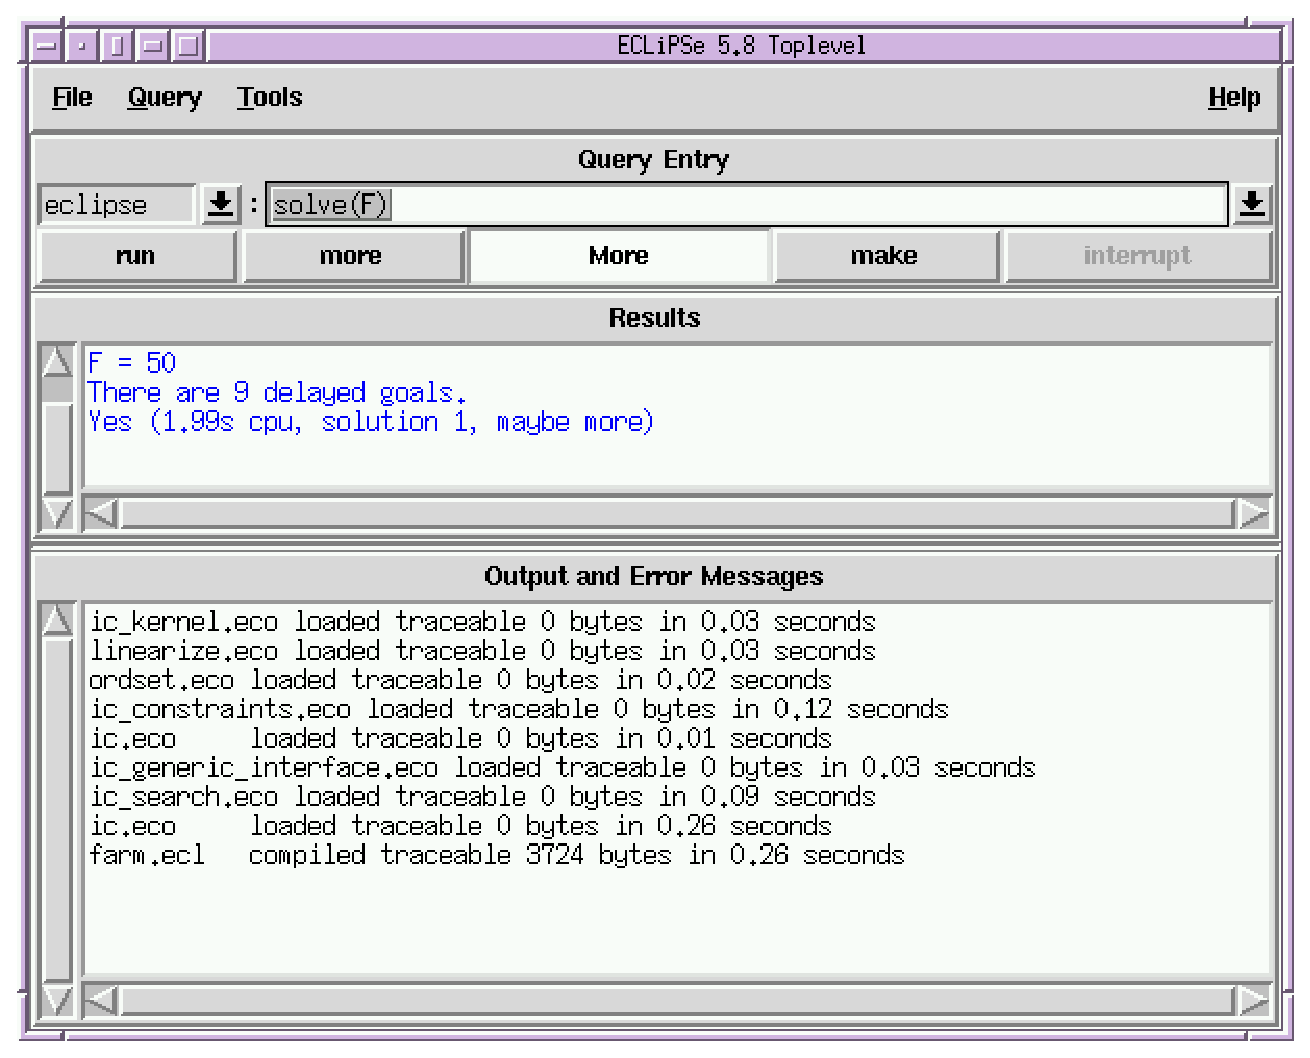
\includegraphics{../userman/tktop.eps}}
\end{center}
\caption{{\tkeclipse} top-level}
\label{tktop}
\end{figure}

Note that help on {\tkeclipse} and its component tools is available
from the \menu{Help} menu in the top-level window.

%------------------------------------------------------------------------
\section{How do I write an {\eclipse} program?}
%------------------------------------------------------------------------
You need to use an editor to write your programs. {\eclipse} does not come
with an editor, but any editor that can save plain text files can be used. 
Save your program as a plain text file, and you can then compile the
program into {\eclipse} and run it.

Extra support for editing {\eclipse} programs with common editors are
available. An eclipse mode for the GNU emacs editor is bundled with the
{\eclipse} package. This mode provides syntax highlighting, automatic
indentation and many other features. To use this mode, you need to load the
\texttt{eclipse.el} file into emacs. This is done by adding the following
line to your \texttt{.emacs} file:

\begin{small}
\begin{verbatim}
(autoload 'eclipse-mode "<eclipsedir>/lib_public/eclipse.el" "ECLIPSE editing mode" t)
\end{verbatim}
\end{small}

where \texttt{<eclipsedir>} is the path to your {\eclipse} installation
directory. 
 
With {\tkeclipse}, you can specify the editor you want to use, and this
editor will be started by {\tkeclipse}, e.g. when you select a file in
the `Edit' option under the File menu. The default values are the value of
the VISUAL environment variable  under Unix, or Wordpad under Windows.
This can be changed with the Preference Editor under the Tools menu.

%------------------------------------------------------------------------
\subsection{Compiling a program}

\index{compile}
From the \menu{File} menu, select the \menuopt{Compile ...} option.
This will bring up a file selection dialogue.  Select the file you wish
to compile, and click on the \button{Open} button.  This will compile
the file and any others it depends on.  Messages indicating which
files have been compiled and describing any errors encountered will be
displayed in the bottom portion of the {\tkeclipse} window
(\guitext{Output and Error Messages}).

If a file has been modified since it was compiled, it may be
recompiled by clicking on the \guitext{make} button.  This recompiles
any files which have become out-of-date.

\See{For more information on program compilation and the compiler,
please see \textbf{The Compiler} chapter in the user manual.}

%------------------------------------------------------------------------
\subsection{Executing a query}

\index{query}
To execute a query, first enter it into the \guitext{Query Entry} text
field.  You will also need to specify which module the query should be
run from, by selecting the appropriate entry from the drop-down list
to the left of the \guitext{Query Entry} field.  Normally, the default
selection of \guitext{eclipse} will be fine; this will allow access to
all {\eclipse} built-ins and all predicates that have not explicitly
been compiled into a different module.  Selecting another module for
the query is only needed if you wish to call a predicate which is not
visible from the {\tt eclipse} module, in which case you need to
select that module.  \See{For more information about the module
system, please see the \textbf{Module System} chapter in the user
manual.}

To actually execute the query, either hit the \keyboard{Enter} key
while editing the query, or click on the \guitext{run} button.
{\tkeclipse} maintains a history of commands entered during the
session, and these may be recalled either by using the drop-down list
to the right of the \guitext{Query Entry} field, or by using the up
and down arrow keys while editing the \guitext{Query Entry} field.

If {\eclipse} cannot find a solution to the query, it will print
\texttt{No} in the \guitext{Results} section of the {\tkeclipse}
window.  If it finds a solution and knows there are no more, it will
print it in the \guitext{Results} section, and then print
\texttt{Yes}.  If it finds a solution and there may be more, it will
print the solution found as before, print \texttt{More}, and enable
the \guitext{more} button.  Clicking on the \guitext{more} button
tells {\eclipse} to try to find another solution.  In all cases it
also prints the total time taken to execute the query.

From \menu{Query} menu, you can run the query with various analysis tools
(see chapter~\ref{sec:program-analysis}): \menuopt{Time Profile} option
will run the query with the profiler tool; \menuopt{Port Profile} option
will run the query with the port profiler tool. 

Note that a query can be interrupted during execution by clicking on
the \guitext{interrupt} button.

%------------------------------------------------------------------------
\subsection{Editing a file}
\label{secedit}

If you wish to edit a file (e.g. a program source file), then you may
do so by selecting the \guitext{Edit ...} option from the
\guitext{File} menu (or use the \guitext{Edit new ...} option if the file
does not yet exist).  This will bring up a file selection dialogue.
Select the file you wish to edit, and click on the \guitext{Open}
button.

When you have finished editing the file, save it.  After you've saved
it, if you wish to update the version compiled into {\eclipse}
(assuming it had been compiled previously), simply click on the
\guitext{make} button.

You can change which program is used to edit your file by using the
{\tkeclipse} Preference Editor, available from the \guitext{Tools}
menu.  Alternatively you can use your editor separately from
\eclipse{}.

%------------------------------------------------------------------------
\subsection{Debugging a program}
\label{secdebug}

To help diagnose problems in {\eclipse} programs, {\tkeclipse}
provides the tracer.  It is activated by selecting the
\guitext{Tracer} option from the \guitext{Tools} menu.  The next time
a goal is executed, the tracer window will become active, allowing you
to step through the program's execution and examine the program's
state as it executes.  A full example is given in
chapter~\ref{chapdebug}.

%------------------------------------------------------------------------
\subsection{File menu}

The \guitext{File} menu of {\tkeclipse} provides various options to
manipulate files:

\subsubsection{Compile} 
Allows the user to select a file to compile into {\eclipse}. 

\subsubsection{Use module}
Allows the user to select and load an {\eclipse} module file into
{\eclipse}.

\subsubsection{Edit} 
Allows the user to select a file to edit using the default text editor 
\See{See section~\ref{secedit} for more information on editors.}.

\subsubsection{Edit new}
Allows the user to specify a new file that will be opened with the default
text editor.

\subsubsection{Cross referencer}
Allows the user to select an {\eclipse} source file and produce a cross
reference over it, and display the resulting graph in a new window.

\subsubsection{Change directory}
Allows the user to change the current working directory.

\subsubsection{Change to example directory}
Change the current working directory to the example directory in the
{\eclipse} distribution.

\subsubsection{New module}
Allows the user to specify a new module that will be created.  The new
module becomes the current toplevel module.  


\subsubsection{Clear toplevel module} 
Allows the user to clear the current toplevel module, i.e. to erase it and
start with a fresh, empty module.

\subsubsection{Exit}
 Leave {\eclipse}


%------------------------------------------------------------------------
\subsection{Getting help}

\index{help}
More detailed help than is provided here can be obtained online for
all the features of {\tkeclipse}.  Simply select the entry from the
\guitext{Help} menu on {\tkeclipse}'s top-level window which
corresponds to the topic or tool you are interested in.

Detailed documentation about all the predicates in the
{\eclipse} libraries can be obtained through the
\guitext{Library Browser and Help} tool.
This tool allows you to browse the online help for the {\eclipse}
libraries.  On the left is a tree display of the libraries available
and the predicates they provide.
\begin{itemize}
\item Double clicking on a node in this tree either expands it or
collapses it again.
\item Clicking on an entry displays help for that entry to the right.
\item Double clicking on a word in the right-hand pane searches for
help entries containing that string.
\end{itemize}
You can also enter a search string or a predicate specification
manually in the text entry box at the top right.  If there is only one
match, detailed help for that predicate is displayed.  If there are
multiple matches, only very brief help is displayed for each; to get
detailed help, try specifying the module and/or the arity of the
predicate in the text field.

Alternatively, you can call the help/1 predicate in the query window
(which contains the same information as the HTML Reference Manual).
It has two modes of operation.  First, when a fragment of a built-in
name is specified, a list of short descriptions of all built-ins whose
name contains the specified string is printed.  For example,
\begin{quote}
\begin{verbatim}
?- help(write).
\end{verbatim}
\end{quote}
will print one-line descriptions about {\bf \tt write/1}, {\bf \tt
writeclause/2}, etc.  When a unique specification is given, the full
description of the specified built-in is displayed, e.g.\ in
\begin{quote}
\begin{verbatim}
?- help(write/1).
\end{verbatim}
\end{quote}
or
\begin{quote}
\begin{verbatim}
?- help(ic:alldifferent/1).
\end{verbatim}
\end{quote}


%------------------------------------------------------------------------
\subsection{Other tools}

{\tkeclipse} comes with a number of useful tools.  Some have been
mentioned above, but here is a more complete list.  Note that we only
provide brief descriptions here; for more details, please see the
online help for the tool in question.

\subsubsection{Compile scratch-pad}

This tool allows you to enter small amounts of program code and have
it compiled.  This is useful for quick experimentation, but not for
larger examples or programs you wish to keep, since the source code is
lost when the session is exited.

\subsubsection{Source File Manager}

This tool allows you to keep track of and manage which source files
have been compiled in the current {\eclipse} session.  You can select
files to edit them, or compile them individually, as well as adding
new files.

\subsubsection{Predicate Browser}

This tool allows you to browse through the modules and predicates
which have been compiled in the current session.  It also lets you
alter some properties of compiled predicates.

\subsubsection{Source Viewer}

This tool attempts to display the source code for predicates selected
in other tools.

\subsubsection{Delayed Goals}

This tool displays the current delayed goals, as well as allowing a
spy point to be placed on the predicate and the source code viewed.

\subsubsection{Inspector}

This tool provides a graphical browser for inspecting terms.  Goals
and data terms are displayed as a tree structure.  Sub-trees can be
collapsed and expanded by double-clicking.  A navigation panel can be
launched which provides arrow buttons as an alternative way to
navigate the tree.

Note that while the inspector window is open, interaction with other
{\tkeclipse} windows is disallowed.  This prevents the term from
changing while being inspected.  To continue {\tkeclipse}, the
inspector window must be closed.

\subsubsection{Visualisation Client}

This starts a new Java visualisation client that allows {\eclipse} programs
to be visualised with the visualisation tools. See the Visualisation manual
for details on the visualisation tools.

\subsubsection{Global Settings}

This tool allows the setting of some global flags governing the way
{\eclipse} behaves.  See also the documentation for the
\bipref{set_flag/2}{../bips/kernel/env/set_flag-2.html} and
\bipref{get_flag/2}{../bips/kernel/env/get_flag-2.html} predicates.

\subsubsection{Statistics}

This tool displays some statistics about memory and CPU usage of the
{\eclipse} system, updated at regular intervals.  See also the
documentation for the
\bipref{statistics/0}{../bips/kernel/env/statistics-0.html} and
\bipref{statistics/2}{../bips/kernel/env/statistics-2.html}
predicates.

\subsubsection{Preference Editor}

This tool allows you to edit and set various user preferences. This
include parameters for how {\tkeclipse} will start up, e.g. the amount
of memory it will be able to use, and a initial query to execute; and
parameters which affects the appearance of {\tkeclipse}, such as the
fonts {\tkeclipse} uses and which editor it launches.


%------------------------------------------------------------------------
\section{How do I make things happen at compile time?}
%------------------------------------------------------------------------

A file being compiled may contain queries.  These are goals
\index{query} preceded by either the symbol ``?-'' or the symbol
``:-''.  As soon as a query or command is encountered in the
compilation of a file, the {\eclipse} system will try to satisfy it.
Thus by inserting goals in this fashion, things can be made to happen
at compile time.

In particular, a file can contain a directive to the system to compile
another file, and so large programs can be split between files, while
still only requiring a single simple command to compile them.
\index{compilation!nesting compile commands} When this happens,
{\eclipse} interprets the pathnames of the nested compiled files
relative to the directory of the parent compiled file; if, for
example, the user calls
\begin{quote}
\begin{verbatim}
[eclipse 1]: compile('src/pl/prog').
\end{verbatim}
\end{quote}
and the file src/pl/prog.pl contains a query
\begin{quote}
\begin{verbatim}
:- [part1, part2].
\end{verbatim}
\end{quote}
then the system searches for the files {\tt part1.pl} and {\tt
part2.pl} in the directory {\tt src/pl} and not in the current
directory.  Usually larger {\eclipse} programs have one main file
which contains only commands to compile all the subfiles.  In
{\eclipse} it is possible to compile this main file from any
directory.  (Note that if your program is large enough to warrant
breaking into multiple files (let alone multiple directories), it is
probably worth turning the constituent components into modules.)
\See{See section~\ref{secmodules} for more information about modules.}

%------------------------------------------------------------------------
\section{How do I use {\eclipse} libraries in my programs?}
\index{libraries}
%------------------------------------------------------------------------

A number of files containing library predicates are supplied with the
{\eclipse} system.  They are usually installed in an {\eclipse}
library directory.  These predicates are either loaded automatically
by {\eclipse} or may be loaded ``by hand''.

During the execution of an {\eclipse} program, the system may
dynamically load files containing library predicates. When this
happens, the user is informed by a compilation or loading message.  It
is possible to explicitly force this loading to occur by use of the
\bipref{lib/1}{../bips/kernel/compiler/lib-1.html} or
\bipref{use_module/1}{../bips/kernel/modules/use_module-1.html}
predicates.  E.g.\ to load the library called {\tt lists}, use one of
the following goals:
\begin{quote}
\begin{verbatim}
:- lib(lists)
:- use_module(library(lists))
\end{verbatim} 
\end{quote}
This will load the library file unless it has been already loaded.  In
particular, a program can ensure that a given library is loaded when
it is compiled, by including an appropriate directive in the source,
e.g.\ {\tt :- lib(lists).}


%------------------------------------------------------------------------
\section{Other tips}
%------------------------------------------------------------------------
\subsection{Recommended file names}

It is recommended programming practice to give the Prolog source
programs the suffix {\bf .pl}, or {\bf .ecl} if it contains {\eclipse}
specific code.  It is not enforced by the system, but it simplifies
managing the source programs.  The
\bipref{compile/1}{../bips/kernel/compiler/compile-1.html} predicate
automatically adds the suffix to the filename, so that it does not
need to be specified; if the literal filename can not be found, the
system tries appending each of the valid suffixes in turn and tries to
find the resulting filename.


%HEVEA\cutend

% BEGIN LICENSE BLOCK
% Version: CMPL 1.1
%
% The contents of this file are subject to the Cisco-style Mozilla Public
% License Version 1.1 (the "License"); you may not use this file except
% in compliance with the License.  You may obtain a copy of the License
% at www.eclipse-clp.org/license.
% 
% Software distributed under the License is distributed on an "AS IS"
% basis, WITHOUT WARRANTY OF ANY KIND, either express or implied.  See
% the License for the specific language governing rights and limitations
% under the License. 
% 
% The Original Code is  The ECLiPSe Constraint Logic Programming System. 
% The Initial Developer of the Original Code is  Cisco Systems, Inc. 
% Portions created by the Initial Developer are
% Copyright (C) 2006 Cisco Systems, Inc.  All Rights Reserved.
% 
% Contributor(s): 
% 
% END LICENSE BLOCK

\chapter{Prolog Introduction}
%HEVEA\cutdef[1]{section}


\section{Terms and their data types}
\index{term} \index{types}
Prolog data ({\bf terms}) and programs are built from a small set of
simple data-types.  In this section, we introduce these data types
together with their syntax (their textual representations).  For the
full syntax see the User Manual appendix on Syntax.

%Syntactically, even the program code itself is made from valid
%Prolog data-structures, which makes so-called meta-programming
%(which means to treat programs as data) easy.

%We shall first introduce
%the various data types, and then describe how Prolog programs can be built.


\subsection{Numbers}
\index{types!integer} \index{integer numbers}
\index{number}
Numbers come in several flavours. The ones that are familiar from
other programming languages are integers and floating point numbers.
Integers in {\eclipse} can be as large as fits into the machine's
memory:
\begin{quote}\begin{verbatim}
123  0   -27   3492374892749289174
\end{verbatim}\end{quote}
\index{types!float} \index{floating point numbers}
Floating point numbers (represented as IEEE double floats) are written
as
\begin{quote}\begin{verbatim}
0.0 3.141592653589793 6.02e23 -35e-12 -1.0Inf
\end{verbatim}\end{quote}
\index{types!rational} \index{rational numbers} \index{types!bounded
real} \index{bounded reals}
{\eclipse} provides two additional numeric types, rationals and
bounded reals.  {\eclipse} can do arithmetic with all these numeric
types.

Note that performing arithmetic requires the use of the \index{is/2}
\bipref{is/2}{../bips/kernel/arithmetic/is-2.html} predicate:

\begin{quote}\begin{verbatim}
?- X is 3 + 4.
X = 7
Yes
\end{verbatim}\end{quote}

\index{=/2}
If one just uses \bipref{=/2}{../bips/kernel/termcomp/E-2.html},
\eclipse{} will simply construct a term corresponding to the
arithmetic expression, and will not evaluate it:

\begin{quote}\begin{verbatim}
?- X = 3 + 4.
X = 3 + 4
Yes
\end{verbatim}\end{quote}

\See{For more details on numeric types and arithmetic in general see the
User Manual chapter on Arithmetic.}

\See{For more information on the bounded real numeric type, see
Chapter~\ref{chapreal}.}

%Rational numbers implement the corresponding mathematical
%notion, i.e.\ the ratio of two integers, and are written like
%\begin{quote}\begin{verbatim}
%1_3  -30517578125_32768  0_1
%\end{verbatim}\end{quote}
%Bounded reals are a representation for a real number that lies between
%two floating-point bounds, e.g.
%\begin{quote}\begin{verbatim}
%3.141592653__3.141592654
%\end{verbatim}\end{quote}
%{\eclipse} can do arithmetic with all these numeric types.
%For more details see the User Manual chapter on Arithmetic.


\subsection{Strings}

\index{string} \index{types!string}
Strings are a representation for arbitrary sequences of bytes and are
written with double quotes:
\begin{quote}\begin{verbatim}
"hello"
"I am a string!"
"string with a newline \n and a null \000 character"
\end{verbatim}\end{quote}
Strings can be constructed and partitioned in various ways using
{\eclipse} primitives.


\subsection{Atoms}

\index{atom} \index{types!atom}
Atoms are simple symbolic constants, similar to enumeration type
constants in other languages. No special meaning is attached to them
by the language.  Syntactically, all words starting with a lower case
letter are atoms, sequences of symbols are atoms, and anything in
single quotes is an atom:
\begin{quote}\begin{verbatim}
atom  quark  i486  -*-  ???  'Atom'   'an atom'
\end{verbatim}\end{quote}


\subsection{Lists}

\index{list} \index{types!list}
A list is an ordered sequence of (any number of) elements, each of
which is itself a term. Lists are delimited by square brackets ({\tt [
]}), and elements are separated by a comma. Thus, the following are
lists:
\begin{quote}\begin{verbatim}
[1,2,3]
[london, cardiff, edinburgh, belfast]
["hello", 23, [1,2,3], london]
\end{verbatim}\end{quote}
\index{empty list} \index{nil@\textit{nil}}
A special case is the empty list (sometimes called {\em nil}), which
is written as
\begin{quote}\begin{verbatim}
[]
\end{verbatim}\end{quote}
A list is actually composed of head-and-tail pairs, where the head contains one
list element, and the tail is itself a list (possibly the empty list).
Lists can be written as a {\tt [Head|Tail]} pair, with the head separated from
the tail by the vertical bar. Thus the list {\tt [1,2,3]} can
be written in any of the following equivalent ways:
\begin{quote}\begin{verbatim}
[1,2,3]
[1|[2,3]]
[1|[2|[3]]]
[1|[2|[3|[]]]]
\end{verbatim}\end{quote}
The last line shows that the list actually consists of 3 {\tt [Head|Tail]}
pairs, where the tail of the last pair is the empty list.
The usefulness of this notation is
that the tail can be a variable (introduced below):
{\tt [1|Tail]}, which leaves the tail unspecified for the moment. 


\subsection{Structures} 

\index{structure} \index{types!structures}
Structures correspond to structs or records in other languages.  A
structure is an aggregate of a fixed number of components, called its
{\em arguments}. Each argument is itself a term.  Moreover, a
structure always has a name (which looks like an atom).  The canonical
syntax for structures is
\begin{quotation}
{\it $<$name$>$($<$arg$>_{1}$,...$<$arg$>_{n}$)}
\end{quotation}
Valid examples of structures are:
\begin{quote}\begin{verbatim}
date(december, 25, "Christmas")
element(hydrogen, composition(1,0))
flight(london, new_york, 12.05, 17.55)
\end{verbatim}\end{quote}
\index{arity} The number of arguments of a structure is called its {\em
arity}.  \index{functor} The name and arity of a structure are
together called its {\em functor} and is often written as {\em
name/arity}.  The last example above therefore has the functor {\tt
flight/4}.

\See{See section \ref{structures} for information about defining structures
with named fields.}

\subsubsection{Operator Syntax} 
\index{operator syntax}
\index{infix}
\index{prefix}
\index{postfix}
As a syntactic convenience, unary (1-argument) structures can also be written
in prefix or postfix notation, and binary (2-argument) structures can be
written in prefix or infix notation, if the programmer has made an
appropriate declaration (called an {\em operator declaration})
about its functor.  For example if {\tt plus/2} were declared to
be an infix operator, we could write:
\begin{quote}\begin{verbatim}
1 plus 100
\end{verbatim}\end{quote}
instead of
\begin{quote}\begin{verbatim}
plus(1,100)
\end{verbatim}\end{quote}
It is worth keeping in mind that the data term represented by the
two notations is the same, we have just two ways of writing the same thing.
Various logical and arithmetic functors are automatically declared to
allow operator syntax, for example {\tt +/2, not/1} etc.

\subsubsection{Parentheses} 
When prefix, infix and postfix notation is used, it is sometimes necessary to
write extra parentheses to make clear what the structure of the written
term is meant to be. For example to write the following nested structure
\begin{quote}\begin{verbatim}
+(*(3,4), 5)
\end{verbatim}\end{quote}
we can alternatively write
\begin{quote}\begin{verbatim}
3 * 4 + 5
\end{verbatim}\end{quote}
because the star binds stronger than the plus sign.
But to write the following differently nested structure
\begin{quote}\begin{verbatim}
*(3, +(4, 5))
\end{verbatim}\end{quote}
in infix-notation, we need extra parentheses:
\begin{quote}\begin{verbatim}
3 * (4 + 5)
\end{verbatim}\end{quote}
A full table of the predefined prefix, infix and postfix operators
with their relative precedences can be found in the appendix of the
User Manual.

\quickref{Summary of Data Types}{
\begin{description}
\item[Numbers]
        \eclipse has {\em integers}, {\em floats}, {\em rationals} and {\em bounded reals}.
\item[Strings]
        Character sequences in double quotes.
\item[Atoms]
        Symbolic constants, usually lower case or in single quotes.
\item[Lists]
        Lists are constructed from cells that have an arbitrary head and
        a tail which is again a list.
\item[Structures]
        Structures have a name and a certain number ({\em arity}) of arbitrary arguments.
        This characteristic is called the {\em functor}, and written name/arity.
\end{description}
}


\section{Predicates, Goals and Queries}

\index{predicate}
\index{goal}
\index{query}
Where other programming languages have procedures and functions,
Prolog and {\eclipse} have {\em predicates}.  A predicate is something
that has a truth value, so it is similar to a function with a boolean result.
A predicate {\em definition} simply defines what is true.
A predicate {\em invocation} (or {\em call}) checks whether something is true or false.
\index{integer/1}
A simple example is the predicate {\em integer/1}, which has a built-in
definition. It can be called to check whether something is an integer:
\begin{quote}\begin{verbatim}
integer(123)           is true
integer(atom)          is false
integer([1,2])         is false
\end{verbatim}\end{quote}
A predicate call like the above is also called a {\em goal}.
A starting goal that the user of a program provides is called a {\em query}.
To show queries and their results, we will from now on
use the following notation:
\begin{quote}\begin{verbatim}
?- integer(123).
Yes.
?- integer(atom).
No.
?- integer([1,2]).
No.
\end{verbatim}\end{quote}
A query can simply be typed at the eclipse prompt, or entered into the
query field in a tkeclipse window. Note that it is not necessary to enter
the {\tt ?-} prefix.
On a console input, is however necessary to terminate the query with a
full-stop (a dot followed by a newline).
After executing the query, the system will print one of the
answers {\bf Yes} or {\bf No}.


\subsection{Conjunction and Disjunction}
\index{conjunction}
\index{disjunction}

\index{conjunction} \index{disjunction}
Goals can be combined to form conjunctions (AND) or disjunctions (OR).
Because this is so common, Prolog uses the comma for AND and the
semicolon for OR. The following shows two examples of conjunction,
the first one is true because both conjuncts are true, the second is false:
\begin{quote}\begin{verbatim}
?- integer(5), integer(7).
Yes.
?- integer(5), integer(hello).
No.
\end{verbatim}\end{quote}
In contrast, a disjunction is only false if both disjuncts are false:
\begin{quote}\begin{verbatim}
?- ( integer(hello) ; integer(5) ).
Yes.
?- ( integer(hello) ; integer(world) ).
No.
\end{verbatim}\end{quote}
As in this example, it is advisable to always surround disjunctions with
parentheses. While not strictly necessary in this example, they are often
required to clarify the structure.

In practice, when answering queries with disjunctions, the system will
actually give a separate {\bf Yes} answer for every way in which the
query can be satisfied (i.e.\ proven to be true).
For example, the following disjunction can be satisfied in two ways,
therefore system will give two {\bf Yes} answers:
\begin{quote}\begin{verbatim}
?- ( integer(5) ; integer(7) ).
Yes (0.00s cpu, solution 1, maybe more)
Yes (0.02s cpu, solution 2)
\end{verbatim}\end{quote}
The second answer will only be given after the user has explicitely
asked for more solutions.
Sometimes the system cannot decide whether an answer is the last one.
In that case, asking for more solutions may lead to an alternative
{\bf No} answer, like in the following example:
\begin{quote}\begin{verbatim}
?- ( integer(5) ; integer(hello) ).
Yes (0.00s cpu, solution 1, maybe more)
No (0.02s cpu)
\end{verbatim}\end{quote}
Of course, as long as there was at least one {\bf Yes} answer, the query
as a whole was true.


\section{Unification and Logical Variables}

\subsection{Symbolic Equality}
\index{equality!symbolic}
Prolog has a particularly simple idea of {\bf equality}, namely
structural equality by pattern matching.  This means that two terms
are equal if and only if they have exactly the same structure.  No
evaluation of any kind is perfomed on them:
\begin{quote}\begin{verbatim}
?- 3 = 3.
Yes.
?- 3 = 4.
No.
?- hello = hello.
Yes.
?- hello = 3.
No.
?- foo(a,2) = foo(a,2).
Yes.
?- foo(a,2) = foo(b,2).
No.
?- foo(a,2) = foo(a,2,c).
No.
?- foo(3,4) = 7.
No.
?- +(3,4) = 7.
No.
?- 3 + 4 = 7.
No.
\end{verbatim}\end{quote}
Note in particular the last two examples (which are equivalent):
there is no automatic arithmetic evaluation. The term +(3,4) is simply
a data structure with two arguments, and therefore of course different from
any number.

Note also that we have used the built-in predicate =/2, which exactly
implements this idea of equality.


\subsection{Logical Variables}
\index{logical variable}

\index{variables} \index{logical variables}
So far we have only performed tests, giving only Yes/No results.
How can we compute more interesting results? 
The solution is to introduce Logical Variables. 
It is very important to understand that Logical Variables are
variables in the mathematical sense, not in the usual programming
language sense. Logical Variables are simply placeholders for
values which are not yet known, like in mathematics.
In conventional programming languages on the other hand, variables
are labels for storage locations.
The important difference is that the value of a logical variables is
typically unknown at the beginning, and only becomes
known in the course of the computation. Once it is known, the variable is just
an alias for the value, i.e. it refers to a term.
Once a value has been assigned to a logical variable, it remains fixed
and cannot be assigned a different value. 

Logical Variables are written beginning with an upper-case letter or
an underscore, for example
\begin{quote}\begin{verbatim}
X   Var   Quark   _123   R2D2
\end{verbatim}\end{quote}
If the same name occurs repeatedly in the same input term (e.g. the same
query or clause), it denotes the same variable.


\subsection{Unification}
\index{unification}

\index{unification} \index{instantiation} \index{aliasing} \index{binding}
With logical variables, the above equality tests become much more interesting,
resulting in the concept of {\em Unification}.
Unification is an extension of the idea of pattern matching of two terms.
In addition to matching, unification also causes the binding (instantiation,
aliasing) of variables in the two terms.
Unification instantiates variables such that the two unified terms become
equal. For example
\begin{quote}\begin{verbatim}
X = 7                is true with X instantiated to 7
X = Y                is true with X aliased to Y (or vice versa)
foo(X) = foo(7)      is true with X instantiated to 7
foo(X,Y) = foo(3,4)  is true with X instantiated to 3 and Y to 4
foo(X,4) = foo(3,Y)  is true with X instantiated to 3 and Y to 4
foo(X) = foo(Y)      is true with X aliased to Y (or vice versa)
foo(X,X) = foo(3,4)  is false because there is no possible value for X
foo(X,4) = foo(3,X)  is false because there is no possible value for X
\end{verbatim}\end{quote}



\quickref{Basic Terminology}{
\begin{description}
\item[Predicate] Something that is true or false, depending on its definition
    and its arguments. Defines a relationship between its arguments.
\item[Goal] A logical formula whose truth value we want to know.
    A goal can be a conjunction or disjunction of other (sub-)goals.
\item[Query] The initial Goal given to a computation.
\item[Unification] An extension of pattern matching which can bind logical
    variables (placeholders) in the matched terms to make them equal.
\item[Clause] One alternative definition for when a predicate is true.
    A clause is logically an implication rule.
\end{description}
}





\section{Defining Your Own Predicates}

\subsection{Comments}
\index{comment}
       Since we will annotate some of our programs, we first introduce
       the syntax for comments. There are two types:
       \begin{description}
        \item[Block comment] The comment is enclosed between the delimiters {\tt /*} and {\tt */}.
         Such comments can span multiple lines, and may be conveniently used
         to comment out unused code.
       \item[Line comment] Anything following and including '{\tt \%}' in a line is taken as a
       comment (unless 
        the '{\tt \%}' character is part of a quoted atom or string).
       \end{description}

\subsection{Clauses and Predicates}
\label{syntax}
\index{clause}

     \index{clause} \index{predicate}
     Prolog programs are built from valid Prolog data-structures.
     A program is a collection of {\it predicates}, and a
     predicate is a collection of {\it clauses}.

     The idea of a clause is to define that something is true.
     The simplest form of a clause is the {\em fact}.
     For example, the following two are facts:
\begin{code}
capital(london, england).
brother(fred, jane).
\end{code}
     Syntactically, a fact is just a structure (or an atom)
     terminated by a full stop.

     Generally, a clause has the form
     \begin{quote}
     Head :- Body.
     \end{quote}
     where {\em Head} is a structure (or atom) and {\em Body} is a {\em Goal},
     possibly with conjunctions and disjunctions like in the queries discussed above.
     The following is a clause
\begin{code}
uncle(X,Z) :- brother(X,Y), parent(Y,Z).
\end{code}
     Logically, this can be read as a reverse implication
     \begin{quote}
     $uncle(X,Z) \longleftarrow brother(X,Y) \wedge parent(Y,Z)$
     \end{quote}
     or, more precisely
     \begin{quote}
     $\forall X \forall Z: uncle(X,Z) \longleftarrow \exists Y: brother(X,Y) \wedge parent(Y,Z)$
     \end{quote}
     stating that uncle(X,Z) is true if brother(X,Y) and parent(Y,Z) are true.
     Note that a fact is equivalent to a clause where the body is {\tt true}:
\begin{code}
brother(fred, jane) :- true.
\end{code}

     One or multiple clauses with the same head functor (same name and number
     of arguments) together form the {\em definition}
     of a predicate. Logically, multiple clauses are read as a disjunction,
    i.e.\ they define alternative ways in which the predicate can be true.
     The simplest case is a collection of alternative facts:
\begin{code}
parent(abe, homer).
parent(abe, herbert).
parent(homer, bart).
parent(marge, bart).
\end{code}
The following defines the ancestor/2 predicate by giving two alternative
clauses (rules):
\begin{code}
ancestor(X,Y) :- parent(X,Y).
ancestor(X,Y) :- parent(Z,Y), ancestor(X,Z).
\end{code}
       Remember that a clause can be read logically, with the {\tt :-}
       taking the meaning of implication, and the comma
       separating goals read as a conjunction. The logical
       reading for several clauses of the same predicate is disjunction
       between the clauses. So the first
       ancestor rule above states that if X is a parent of Y, then this
       implies that X is an ancestor of Y. The second rule, which specifies
       another way X can be an ancestor of Y states that if some other
       person, Z, is the parent of Y, {\it and\/} X is an ancestor of Z,
       then this implies that X is also an ancestor of Y.

%       In fact, syntactically, the {\tt ':-'} and {\tt ','} used in 
%       constructing clauses are operators ({\tt :-/2} and {\tt ,/2}
%       if a clause contains more than two body goals, this is achieved by
%       nesting of {\tt ,/2}).

\Note{
\index{variables!scope}
It is also important to remember that the scope of a variable
       name only extends over the clause in which it is in, so any
       variables with the same name in the same clause refer to the
       same variable, but variables which occur in different clauses
       are different even if they have been written with the same name.
       }


\section{Execution Scheme}

%       Before we describe the execution of Prolog programs in more detail, we
%       shall first discuss the basic mechanism for computation in Prolog --
%       unification.  
%
%\subsection{Unification}
%
%  Unification is the pattern matching of two terms. In addition to
%  matching, unification also causes the binding (aliasing) of
%  variables in the two terms. For example,
%  \begin{quotation}
%  unifying {\tt capital(london,Country) } with {\tt capital(london,england)} will
%  cause {\tt Country} to bind to 
%  {\tt england}.
%  \end{quotation}
%
%   Note that variables from the two terms being unified can both supply
%   variables that are bound, e.g. unifying
%
%\begin{verbatim}
%   capital(City,england)      capital(london, Country)
%\end{verbatim}
%
%   would bind {\tt City} to {\tt london}, and {\tt Country} to {\tt england}.
%
%   If the two terms being unified do not match with each other, then the 
%   unification {\bf fails}. Here are examples of pairs of terms that fail
%   to unify:
%\begin{verbatim}
%
%       london                    france
%       capital(City,Country)     ancestor(X,Y)
%       capital(london, Country)  capital(paris, Country)
%
%\end{verbatim}
%

\subsection{Resolution}
\index{resolution}

\index{resolution} \index{resolvent}
Resolution is the computation rule used by Prolog. Given a set of
facts and rules as a program, execution begins with a query, which is
an initial goal that is to be resolved.
The set of goals that still have to be resolved is called the
{\em resolvent}.

Consider again the {\tt ancestor/2}
and {\tt parent/2} predicate shown above.
\begin{code}
ancestor(X,Y) :- parent(X,Y).                 % clause 1
ancestor(X,Y) :- parent(Z,Y), ancestor(X,Z).  % clause 2 

parent(abe, homer).                           % clause 3
parent(abe, herbert).                         % clause 4
parent(homer, bart).                          % clause 5
parent(marge, bart).                          % clause 6
\end{code}
Program execution is started by issuing a query, for example
\begin{quote}\begin{verbatim}
?- ancestor(X, bart).
\end{verbatim}\end{quote}
This is our initial resolvent.
The execution mechanism is now as follows:
\exercises{Execution Algorithm}{
\begin{enumerate}
\item Pick one (usually the leftmost) goal from the resolvent.
        If the resolvent is empty, stop.
\item Find all clauses whose head successfully unifies with this goal.
        If there is no such clause, go to step 6.
\item Select the first of these clause. If there are more, remember the
        remaining ones. This is called a {\em choice point}.
\item Unify the goal with the head of the selected clause.
        (this may instantiate variables both in the goal and in the clause's body).
\item Prefix this clause body to the resolvent and go to 1.
\item \index{backtracking}
      Backtrack: Reset the whole computation state to
        how it was when the most recent choice point was created.
        Take the clauses remembered in this choice point and go to 3.
\end{enumerate}
}
In our example, the Prolog system would attempt to unify
{\tt ancestor(X, bart)} with the program's
clause heads. Both clauses of the {\tt ancestor/2} predicate can
unify with the goal, but the textually first clause, clause 1, is
selected first, and successfully unified with the goal:
\begin{quote}\begin{verbatim}
Goal (Query):   ancestor(X,bart)
Selected:       clause 1
Unifying:       ancestor(X,bart) = ancestor(X1,Y1)
results in:     X=X1, Y1=bart
New resolvent:  parent(X, bart)
More choices:   clause 2
\end{verbatim}\end{quote}
The body goal of clause 1 \verb'parent(X, bart)' is added to the
resolvent, and the system remembers that there is an untried 
alternative -- this is referred to as a {\it choice-point}.

In the same way, \verb'parent(X, bart)' is next selected for 
unification. Clauses 5 and 6 are possible matches for this goal,
with clause 5 selected first. There are no body goals to add, and
the resolvent is now empty:
\begin{quote}\begin{verbatim}
Goal:           parent(X, bart)
Selected:       clause 5
Unifying:       parent(X,bart) = parent(homer,bart)
results in:     X = homer
New resolvent:  
More choices:   clause 6, then clause 2
\end{verbatim}\end{quote}
The execution of a program completes successfully when there is an
empty resolvent. The program has thus found the first solution 
to the query, in the form of instantiations to the original Query's
variables, in this case {\tt X = homer}. \eclipse\ returns this
solution, and also asks if we want more solutions:
\begin{quote}\begin{verbatim}
?- ancestor(X,bart).
X = homer     More? (;) 
\end{verbatim}\end{quote}
Responding with ';' will cause \eclipse\ to try to find alternative
solutions by {\bf backtracking} to
the most recent choice-point, i.e. to seek an alternative to 
{\tt parent/2}. Any bindings done during and after the selection of 
clause 5 are undone, i.e. the binding of  X to {\tt 
homer} is undone. Clause 6 is now unified with
the goal {\tt parent(X,Y)}, which again produces a solution:
\begin{quote}\begin{verbatim}
Goal:           parent(X, bart)
Selected:       clause 6
Unifying:       parent(X,bart) = parent(marge,bart)
results in:     X = marge
New resolvent:  
More choices:   clause 2
\end{verbatim}\end{quote}
If yet further solutions are needed, then \eclipse\ would again backtrack.
This time, {\tt parent/2} no longer has any alternatives left to unify,
so the next older choice-point, the one made for {\tt ancestor/2},
is the one that would be considered. The computation is returned
to the state it was in just before clause 1 was selected, and clause 2
is unified with the query goal:
\begin{quote}\begin{verbatim}
Goal:           ancestor(X,bart)
Selected:       clause 2
Unifying:       ancestor(X,bart) = ancestor(X1,Y1)
results in:     Y1 = bart, X1 = X
New resolvent:  parent(Z1, bart), ancestor(X1, Z1)
More choices:   
\end{verbatim}\end{quote}
For the first time, there are more than one goal in the resolvent, the
leftmost one, {\tt parent(Z1,bart)} is then
selected for unification. Again, clauses 5 and 6 are candidates, and
a new choice-point is created, and clause 5 tried first.
\begin{quote}\begin{verbatim}
Goal:           parent(Z1, bart)
Selected:       clause 5
Unifying:       parent(Z1, bart) = parent(homer, bart)
results in:     Z1 = homer
New resolvent:  ancestor(X1, homer)
More choices:   clause 6
\end{verbatim}\end{quote}
Eventually, after a few more steps
(via finding the ancestor of {\tt homer}), this leads to a new solution, 
with {\tt abe} returned as an ancestor of {\tt bart}:
\begin{quote}\begin{verbatim}
?- ancestor(X,bart).
X = abe     More? (;) 
\end{verbatim}\end{quote}
If yet more solutions are requested, then because only one parent for
{\tt homer} is given by the program, \eclipse\ would backtrack to the only 
remaining choice-point, unifying clause 6 is unified with the goal, 
binding \verb'Z1' to \verb'marge'. However, no ancestor for {\tt marge}
can be found, because no parent of
{\tt marge} is specified in the program. No more choice-points remains to
be tried, so the execution terminates.



\section{Partial data structures}
\label{tail}
\index{tail}
Logical variables can occur anywhere, not only as arguments of clause
heads and goals, but also within data structures.
A data structure which contains variables is called a partial data
structure, because it will eventually be completed by substituting
the variable with an actual data term.
The most common case of a partial data structure is a list whose
tail is not yet instantiated.

Consider first an example where no partial lists occur.
In the following query, a list is built incrementally,
starting from its end:
\begin{quote}\begin{verbatim}
?- L1 = [], L2 = [c|L1], L3 = [b|L2], L4 = [a|L3].
L1 = []
L2 = [c]
L3 = [b, c]
L4 = [a, b, c]
\end{verbatim}\end{quote}
Whenever a new head/tail cell is created,
the tail is already instantiated to a complete list.

But it is also possible to build the list from the front.
The following code, in which the goals have been reordered,
gives the same final result as the code above:
\begin{quote}\begin{verbatim}
?- L4 = [a|L3], L3 = [b|L2], L2 = [c|L1], L1 = [].
L1 = []
L2 = [c]
L3 = [b, c]
L4 = [a, b, c]
\end{verbatim}\end{quote}
However, in the course of the computation, variables get instantiated to
''partial lists'', i.e.\ lists whose head is known, but whose tail is not.
This is perfectly legal: due to the nature of the logical variable, the
tail can be filled in later by instantiating the variable.

%Partial data structures are in fact a very 
%important feature of Prolog. Variables can occur anywhere inside
%a data structure, and this allows data to be built incrementally and dynamically:
% the partially built data structure is passed
%around, and its ``holes'' (the variables) are filled in by further partial
%data structures.

%THIS IS NOT AN EXAMPLE OF PARTIAL DATA STRUCTURES!
%An example use of partial data structure is in the use of accumulator pairs,
%which was demonstrated in section~\ref{tail} with numbers. However, the
%`value' being accumulated can be a partial data structure, as shown with
%this example of reversing a list:
%\begin{code}
%reverse(List,Reverse) :- rev(List, [], Reverse).
%
%rev([], R, R).
%rev([E|L], R0, R) :- rev(L, [E|R0], R).
%\end{code}
%
%The partially reversed list is being constructed in the second argument of
%\verb'rev/3', and finally passed out when the end of the list is reached.


%\subsection{Difference Lists}
%An important technique using partial data structure is the difference list.
%In difference lists, a list is represented by a pair of (perhaps partial)
%lists, e.g.
%the list \verb'[1,2,3|T]' can be represented as the pair \verb'[1,2,3|T]' and
%\verb'T'. This gives direct access to the tail of a list, and the list does
%not need to be traversed to reach the tail. This can result in much improved
%efficiency when, for example, appending two lists together. With a normal
%list representation, the {\tt append} predicate is written as:
%\begin{code}
%% append(L1, L2, L) L is the list L2 appended to the end of L1
%append([], L, L).
%append([E|L1], L2, [E|L]) :-
%    append(L1, L2, L).
%\end{code}
%
%With this encoding, the first list has to be traversed fully to find
%the end, and then the 
%second list appended to that.
%
%With the difference list representation, the end of the lists are known,
%and the append can be encoded with a simple fact:
%\begin{code}
%/* append_dl(L1,E1, L2,E2, L,E) 
%   L,E is the appended list of L1,E1 and L2,E2 
%*/
%append_dl(L1,E1, E1,E2, L1,E2).
%\end{code}
%
%\begin{figure}
%%\epsfbox{appenddiff.ps}
%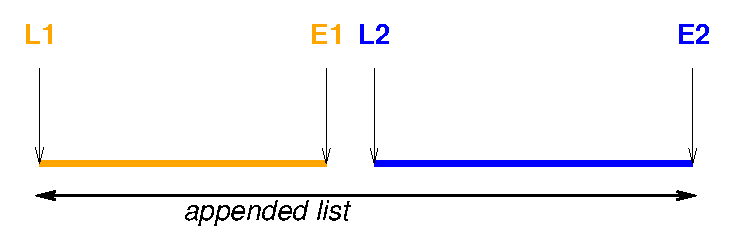
\includegraphics{appenddiff.ps}
%\caption{Appending difference lists}
%\end{figure}
%The situation is as shown in the figure. By setting E1 to L2, the second 
%list is appended to the end of the first list, and \verb'L1',\verb'E2' now
%represents the combined list. With this difference list representation,
%no traversal of the first list is needed, and the operation is done in
%constant time. It can thus be much more efficient, especially if the first
%list is long.

\section{More control structures}
    \subsection{Disjunction}
\index{disjunction} \index{;/2}
Disjunction is normally specified in Prolog by different clauses of
a predicate, but it can also be specified within a single clause by
the use of \verb';/2'. For example,

\begin{code}
atomic_particle(X) :- (X = proton ; X = neutron ; X = electron).
\end{code}

This is logically equivalent to: 

\begin{code}
atomic_particle(proton).
atomic_particle(neutron).
atomic_particle(electron).
\end{code}

    \subsection{Conditional}

\index{conditional} \index{->/2}
Conditionals can be specified using the \verb'->/2' operator.
In combination with \verb';/2', a conditional similar to `if-then-else' 
constructs of conventional language can be constructed:
\verb'X->Y;Z', where \verb'X', \verb'Y' and \verb'Z' can be one or more
goals,  means that if \verb'X' is true, then \verb'Y' will be
executed, otherwise \verb'Z'. Only the first solution of \verb'X' is
explored, so that on backtracking, no new solutions for \verb'X' will be
tried. In addition, if \verb'X' succeeds, then the `else' part, \verb'Z'
will never be tried. If \verb'X' fails, then the `then' part, \verb'Y',
will never be tried. An example of `if-then-else' is:
\begin{code}
max(X,Y, Max) :- 
   number(X), number(Y),
   (X > Y -> Max = X ; Max = Y).
\end{code}
where \verb'Max' is the bigger of the numbers \verb'X' or \verb'Y'.
Note the use of the brackets to make the scope of the if-then-else
clear and correct.


    \subsection{Call} 
\index{call}
\index{metacall}
One feature of Prolog is the equivalence of  programs and data -- both are
represented as terms. The predicate \verb'call' allows 
program terms (i.e. data) to be treated as goals: \verb'call(X)' will cause
\verb'X' to be treated as a goal and executed. Although at the time when 
the predicate is executed, \verb'X' has to be instantiated, it does not 
need to be instantiated (or even known) at compile time. For example, it
would in principle be
possible to define disjunction (\verb';') as follows:

\begin{code}
X ; Y :- call(X).
X ; Y :- call(Y).
\end{code}

%In addition, a Prolog program can construct a term at run-time, which is then 
%called as a goal.  This is sometimes used to ensure goals are compiled
%after earlier goals have already been executed, for
%example\footnote{The 'foreach' construct is described in the next chapter.}:
%\begin{verbatim}
%Y=A, call(foreach(A,[a,b,c]) do writeln(Y)).
%\end{verbatim}
%As required, this means the same as
%\begin{verbatim}
%foreach(A,[a,b,c]) do writeln(A).
%\end{verbatim}


\subsection{All Solutions}
\label{all-solutions}

In the pure computational model of Prolog, alternative solutions are
computed one-by-one on backtracking. Only one solution is available
at any time, while previous solutions disappear on backtracking:
\begin{quote}\begin{verbatim}
?- weekday(X).
X = mo
More
X = tu
More
X = we
More
...
\end{verbatim}\end{quote}
Sometimes it is useful to have all solution together in a list.
This can be achieved by using one of the all-solutions predicates
\index{findall/3}\index{setof/3}\index{bagof/3}findall/3, setof/3 or bagof/3:
\begin{quote}\begin{verbatim}
?- findall(X, weekday(X), List).
X = X
List = [mo, tu, we, th, fr, sa, su]
Yes
\end{verbatim}\end{quote}
\See{For the differences between findall/3, setof/3 and bagof/3
see the \eclipse{} Reference Manual.}


\section{Using Cut}
\label{cut}
\index{cut}
Cut (written as \verb'!') prunes away part of the Prolog search-space. This
can be a very powerful mechanism for improving the performance of programs,
and even the suppression of unwanted solutions. However, it can also be
easily misused and over-used. 

Cut does two things:

\begin{description}
\item[commit] Disregard any later clauses for the predicate.
\item[prune] Throw away all alternative solutions to the goals to the left of
 the cut.
\end{description}

\subsection{Commit to current clause}
\index{commit}

Consider the following encoding of the ``minimum'' predicate:
\begin{code}
min(X,Y, Min) :- X <Y, Min = X.
min(X,Y, Min) :- Y=<X, Min = Y.
\end{code}
Whilst logically correct, the behaviour of this encoding is
non-optimal for two reasons.  Consider the goal {\tt :- min(2,3,M)}.
Although the first clause succeeds, correctly instantiating $M$ to
$2$, Prolog leaves an open choice point.  If these clauses and goal
occur as part of a larger program and goal, a failure might occur
later, causing backtracking to this open choice point. 
Prolog would then, in vain, try to find another minimum using the
second clause for {\tt min}.  So there is a double drawback:
firstly, an open choice point consumes memory, and secondly the
unsuccessful evaluation of the second clause costs execution time.

To achieve the same logic, but more efficient behaviour, the
programmer can introduce a {\it cut}.
For example {\tt min} is typically encoded as follows:
\begin{code}
min(X,Y, Min) :- X<Y, !, Min = X.
min(X,Y, Y).
\end{code}
The cut removes the unnecessary choice point, which means that the
second clause will never be executed if the first clause passed the
cut.  This effectively makes the test in the second clause redundant,
and it can therefore be removed.

  \subsection{Prune alternative solutions}
\index{prune}
A cut may occur anywhere where a goal may occur, consider the following:
\begin{code}
first_prime(X, P) :-
    prime(X,P), !.
\end{code}
where \verb'first_prime' returns the first prime number smaller than \verb'X'.
In this case, it calls a predicate \verb'prime/2', which generates prime
numbers smaller than \verb'X', starting from the largest one. The effect of
the cut here is to prune away all the remaining solutions to \verb'prime(X,P)'
once the first one is generated, so that on backtracking, \verb'prime(X,P)'
is not tried for alternative solutions. The cut will also commit the execution
to this clause for \verb'first_prime/2', but as there is only one clause,
this has no visible effect.


%%----------------------------------------------------------------------
%\section{Prolog vs Imperative Languages}
%%----------------------------------------------------------------------
%\quickref{Comparison Prolog vs Imperative Programming}{
%\begin{tabular}{p{7cm}p{7cm}}
%{\bf Prolog} & {\bf Imperative Language} \\
%\hline
%\hline
%set of clauses & program \\
%\hline
%predicate (set of clauses with same name and arity) & procedure \\
%\hline
%clause (rule or fact) & if statement / one arm of nondeterministic case
%        statement / sequence of procedure calls \\
%\hline
%goal invocation & procedure call \\
%\hline
%unification & parameter passing / assignment / dynamic memory allocation /
%        conditional branching \\
%\hline
%backtracking & continuation passing / exception handling /
%        execution state manipulation \\
%\hline
%logical variable & pointer manipulation \\
%\hline
%tail recursion & iteration \\
%\end{tabular}
%}

%----------------------------------------------------------------------
\section{Common Pitfalls}
%----------------------------------------------------------------------
Prolog is different from conventional programming languages, and a common
problem is to program Prolog like a conventional language. Here are some
points to note:

\begin{itemize}
\item Unification is more powerful than normal case discrimination (see 
  section~\ref{unif}); 
\item Prolog procedure calls are more powerful than conventional procedure
calls. In particular, backtracking is possible (see section~\ref{back});
\end{itemize}

    \subsection{Unification works both ways}
\label{unif}
One common problem is to write a predicate expecting certain instantiation
patterns for the arguments, and then get unexpected results when the 
arguments do not conform to the expected pattern. An example is the
member relation, intended to check if an item \verb'Item' is a member of
a list or not. This might be written as:


\begin{code}
member(Item, [Item|_]).
member(Item, [_|List]) :- member(Item, List).
\end{code}

The expected usage assumes both \verb'Item' and the list are ground. In 
such cases, the above predicate does indeed check if \verb'Item' occurs in
the list given as a second argument. However, if either of the arguments are
not ground, then potentially unexpected behaviour might occur. Consider
the case where \verb'Item' is a variable, then the above predicate will 
enumerate the elements of the list successively through backtracking. On
the other hand, if any of the list elements of the list is a variable, they
would be unified with \verb'Item'. Other instantiation patterns for either
arguments can produce even more complex results. 

If the intended meaning is simply to check if \verb'Item' is a member of 
a list, this can be done by:

\begin{code}
  \% is_member(+Element, +List)
  \% check if Element is an element that occurs in a List of
  \% ground elements
is_member(Item, [Element|_]) :- Item == Element.
is_member(Item, [_|List]) :- nonvar(List), is_member(Item, List).
\end{code}

Note the use of comments to make clear the intention of the use of the
predicate. The convention used is that `+' indicates that an argument should
be instantiated (i.e. not a variable), `-' for an argument that should be
an uninstantiated variable, and '?' indicates that there is no restrictions
on the mode of the argument.

    \subsection{Unexpected backtracking}
\label{back}
Remember that when coding in Prolog, any predicate {\it may\/} be backtracked 
into. So correctness in Prolog requires:

\begin{itemize}
\item Predicate returns the correct answer when first called.
\item Predicate behaves correctly when backtracked into.
\end{itemize}

Recall that backtracking causes alternative choices to be explored, if
there are any.  Typically another choice corresponds to another clause
in the poredicate definition, but alternative choices may come from
disjunction (see above) or built-in predicates with multiple
(alternative) solutions. 
The programmer should make sure that a predicate will only produce
those solutions that are wanted. Excess alternatives can be removed by
coding the program not to produce them, or by the cut, or the conditional.

For example, to return only the {\it first\/} member, in the
\verb'is_member/2' example, 
the predicate can be coded using the cut, as follows:

\begin{code}
is_member(Item, [Element|_]) :- Item == Element, !.
is_member(Item, [_|List]) :- nonvar(List), is_member(Item, List).
\end{code}

\subsubsection{Using conditional}

Another way to remove excess choice points is the conditional:

\begin{code}
is_member(Item, [Element|List]) :- 
    ( Item == Element ->
        true 
    ;
        nonvar(List), is_member(Item, List)
    ).
\end{code}


\section{Exercises}

\begin{enumerate}

\item

Consider again the ``family tree'' example (see Section~\ref{syntax}).
As well as the \texttt{parent/2} predicate, suppose we have a
\texttt{male/1} predicate as follows:

\begin{code}
male(abe).
male(homer).
male(herbert).
male(bart).
\end{code}

Define a \texttt{brother/2} predicate, expressed just in terms of
\texttt{parent/2} and \texttt{male/1}.  Make sure Homer is not considered
his own brother.


\item

Consider the following alternative definition of \texttt{ancestor/2}:

\begin{code}
ancestor(X, Y) :- parent(X, Y).
ancestor(X, Y) :- ancestor(X, Z), parent(Z, Y).
\end{code}

What is wrong with this code?  What happens if you use it to find out
who Bart is an ancestor of?

\end{enumerate}

%HEVEA\cutend

% BEGIN LICENSE BLOCK
% Version: CMPL 1.1
%
% The contents of this file are subject to the Cisco-style Mozilla Public
% License Version 1.1 (the "License"); you may not use this file except
% in compliance with the License.  You may obtain a copy of the License
% at www.eclipse-clp.org/license.
% 
% Software distributed under the License is distributed on an "AS IS"
% basis, WITHOUT WARRANTY OF ANY KIND, either express or implied.  See
% the License for the specific language governing rights and limitations
% under the License. 
% 
% The Original Code is  The ECLiPSe Constraint Logic Programming System. 
% The Initial Developer of the Original Code is  Cisco Systems, Inc. 
% Portions created by the Initial Developer are
% Copyright (C) 2006 Cisco Systems, Inc.  All Rights Reserved.
% 
% Contributor(s): 
% 
% END LICENSE BLOCK

\chapter{\eclipse{} Programming}
%HEVEA\cutdef[1]{section}

%----------------------------------------------------------------------
\section{Structure Notation}
\label{structures}
In \eclipse, structure fields can be given names.
This makes it possible to write structures in a
more readable and maintainable way.
Such structures first need to be declared by specifying a template like:   
\begin{code}
:- local struct( book(author, title, year, publisher) ).
\end{code}
Structures with the functor book/4 can then be written as   
\begin{quote}\begin{verbatim}
book{}
book{title:'tom sawyer'}
book{title:'tom sawyer', year:1876, author:twain}
\end{verbatim}\end{quote}
which, in canonical syntax, correspond to the following:
\begin{quote}\begin{verbatim}
book(_, _, _, _)
book(_, 'tom sawyer', _, _)
book(twain, 'tom sawyer', 1876, _)
\end{verbatim}\end{quote}
There is absolutely no semantic difference between the two syntactical forms.
The special struct-syntax with names has the advantage that
\begin{itemize}
\item the arguments can be written in any order
\item ``dummy'' arguments with anonymous variables do not need to be written
\item the arity of the structure is not implied (and can be changed
by changing the declaration and recompiling the program)
\end{itemize}
Sometimes it is necessary to refer to the numerical position of a
structure field within the structure, e.g. in the arg/3 predicate:
\begin{quote}\begin{verbatim}
arg(3, B, Y)
\end{verbatim}\end{quote}
When the structure has been declared as above, we can write instead:
\begin{quote}\begin{verbatim}
arg(year of book, B, Y)
\end{verbatim}\end{quote}

Declared structures help readability, and make programs easier to modify.
In order not to lose these benefits, one should always use curly-bracket and
of-syntax when working with them, and never write them in canonical
syntax or referring to argument positions numerically.

\See{See also the
\bipref{update_struct/4}{../bips/kernel/termmanip/update_struct-4.html}
built-in predicate.}


%----------------------------------------------------------------------
\section{Loops}
\label{sec:loops}
To reduce the need for auxiliary recursive predicates, \eclipse{} allows
the use of an iteration construct
\begin{quote}\begin{verbatim}
( IterationSpecs do Goals )
\end{verbatim}\end{quote}
Typical applications are: Iteration over a list
\begin{quote}\begin{verbatim}
?- ( foreach(X,[1,2,3]) do writeln(X) )
1
2
3
Yes (0.00s cpu)
\end{verbatim}\end{quote}
Process all elements of one list and construct another:
\begin{quote}\begin{verbatim}
?- ( foreach(X,[1,2,3]), foreach(Y,List) do Y is X+3 ).
List = [4, 5, 6]
Yes (0.00s cpu)
\end{verbatim}\end{quote}
Process a list to compute the sum of its elements:
\begin{quote}\begin{verbatim}
?- ( foreach(X,[1,2,3]), fromto(0,In,Out,Sum) do Out is In+X ).
Sum = 6
Yes (0.00s cpu)
\end{verbatim}\end{quote}
Note that the variables X, Y, In and Out are local variables in the loop,
while the input list and Sum are shared with the context.

If a parameter remains constant across all loop iterations it must
be specified explicitly (via {\bf param}),
for example when iterating over an array:
\begin{quote}\begin{verbatim}
?- Array = [](4,3,6,7,8),
   (
       for(I,1,5),
       fromto(0,In,Out,Sum),
       param(Array)
   do
       Out is In + Array[I]
   ).
\end{verbatim}\end{quote}
\quickref{Iteration Specifiers for Loops}{
\begin{description}
\item[fromto(First,In,Out,Last)]\ \\
     iterate Goals starting with In=First until Out=Last.
\item[foreach(X,List)]\ \\
     iterate Goals with X ranging over all elements of List.
\item[foreacharg(X,StructOrArray)]\ \\
     iterate Goals with X ranging over all arguments of StructOrArray.
\item[foreacharg(X,StructOrArray,Idx)]\ \\
     same as before, but Idx is set to the argument position of X in
     StructOrArray.
\item[foreachelem(X,Array)]\ \\
     like foreacharg/2, but iterates over all elements of an array
     of arbitrary dimension.
\item[foreachelem(X,Array,Idx)]\ \\
     same as before, but Idx is set to the index position of X in
     Array.
\item[foreachindex(Idx,Array)]\ \\ 
     like foreachelem/3, but returns just the index position and not the
     element.
\item[for(I,MinExpr,MaxExpr)]\ \\
     iterate Goals with I ranging over integers from MinExpr to MaxExpr.
\item[for(I,MinExpr,MaxExpr,Increment) ]\ \\
     same as before, but Increment can be specified (it defaults to 1). 
\item[multifor(List,MinList,MaxList)]\ \\
     like for/3, but allows iteration over multiple indices (saves
     writing nested loops).
\item[multifor(List,MinList,MaxList,IncrementList)]\ \\
     same as before, but IncrementList can be specified (i.e.\ how
     much to increment each element of List by).
\item[count(I,Min,Max)]\ \\
     iterate Goals with I ranging over integers from Min up to Max.
\item[param(Var1,Var2,...)]\ \\
     for declaring variables in Goals global, i.e.\ shared with the context.
\end{description}
}
\See{For details and more examples see the description of the
\bipref{do/2}{../bips/kernel/control/do-2.html}
built-in predicate. Additional background can be found in \cite{loops02}.}

%----------------------------------------------------------------------

\section{Working with Arrays of Items}

For convenience, \eclipse{} has some features for facilitating working with
arrays of items.
Arrays can be of any dimension, and can be declared with the
\bipref{dim/2}{../bips/kernel/termmanip/dim-2.html}
predicate:
\begin{quote}\begin{verbatim}
?- dim(M,[3,4]).
M = []([](_131, _132, _133, _134),
       [](_126, _127, _128, _129),
       [](_121, _122, _123, _124))
yes.
\end{verbatim}\end{quote}
\bipref{dim/2}{../bips/kernel/termmanip/dim-2.html} can also be used to
query the dimensions of an array:
\begin{quote}\begin{verbatim}
?- dim(M,[3,4]), dim(M,D).
...
D = [3, 4]
yes.
\end{verbatim}\end{quote}

\Note{Note that arrays are just structures, and that the functor is not
important.}

To access a specific element of an array in an expression, specify the index
list of the desired element, e.g.\
\begin{quote}\begin{verbatim}
?- M = []([](2, 3, 5),
          [](1, 4, 7)),  X is M[1, 2] + M[2, 3].
X = 10
M = []([](2, 3, 5), [](1, 4, 7))
yes.
\end{verbatim}\end{quote}

\quickref{Array notation}{
\begin{itemize}
\item Arrays are just structures
\item The functor is not important
\item Declare or query array size with
        \bipref{dim/2}{../bips/kernel/termmanip/dim-2.html}
\item Access elements in expressions by specifying their index list
        (e.g.\ \texttt{A[7]}, \texttt{M[2,3]})
\item Indices start at 1
\end{itemize}
}

\See{For further details see the Array Notation section of the User Manual.}

%----------------------------------------------------------------------


\section{Storing Information Across Backtracking}

In pure logic programming, the complete state of a computation is
reset to an earlier state on backtracking.
The all-solutions predicates introduced in section \ref{all-solutions}
provide a way to collect solutions across backtracking.

The following section presents \eclipse's lower-level primitives for storing
information across failures: bags and shelves.
Both bags and shelves are referred to by handle, not by name,
so they make it easy to write robust, reentrant code.
Bags and shelves disappear when the system backtracks over their
creation, when the handle gets garbage collected, or when they are
destroyed explicitly.


\subsection{Bags}

A bag is an anonymous object which can be used to store information
across failures.  A typical application is the collection of
alternative solutions.

A bag is an unordered collection, referred to by a handle.
A bag is created using bag_create/1, terms can be added to a bag using
bag_enter/2, and the whole contents of the bag can be retrieved
using bag_retrieve/2 or bag_dissolve/2.
A simple version of the findall/3 predicate from section \ref{all-solutions}
can be implemented like:
\begin{code}
simple_findall(Goal, Solutions) :-
        bag_create(Bag),
        (
            call(Goal),
            bag_enter(Bag, Goal),
            fail
        ;
            bag_dissolve(Bag, Solutions)
        ).
\end{code}


\subsection{Shelves}

A shelf is an anonymous object which can be used to store information
across failures. A typical application is counting of solutions,
keeping track of the best solution, 
aggregating information across multiple solutions etc. 

A shelf is an object with multiple slots whose contents survive
backtracking. The content of each slot can be set and retrieved
individually, or the whole shelf can be retrieved 
as a term. Shelves are referred to by a handle.

A shelf is initialized using shelf_create / 2 or shelf_create /
3. Data is stored in the slots (or the shelf as a whole) with
shelf_set / 3 and retrieved with shelf_get / 3.  

For example, here is a meta-predicate to count the number of solutions
to a goal: 
\begin{code}
count_solutions(Goal, Total) :-
    shelf_create(count(0), Shelf),
    (
        call(Goal),
        shelf_get(Shelf, 1, Old),
        New is Old + 1,
        shelf_set(Shelf, 1, New),
        fail
    ;
        shelf_get(Shelf, 1, Total)
    ),
    shelf_abolish(Shelf).
\end{code}


%----------------------------------------------------------------------


%----------------------------------------------------------------------
\section{Input and Output}
%----------------------------------------------------------------------

\subsection{Printing {\eclipse} Terms}
\quickref{Builtins for writing}{
\begin{description}
\item[write(+Stream, ?Term)]\ \\
        write one term in a default format.
\item[write_term(+Stream, ?Term, +Options)]\ \\
        write one term, format options can be selected.
\item[printf(+Stream, +Format, +ArgList)]\ \\
        write a string with embedded terms, according to a format string.
\item[writeq(+Stream, ?Term), write_canonical(+Stream, ?Term)]\ \\
        write one term so that it can be read back.
\item[put(+Stream, +Char)]\ \\
        write one character.
\end{description}
}
The predicates of the write-group are generic in the sense that they
can print any {\eclipse} data structure.
The different predicates print slightly different formats.
The {\tt write/1} predicate is intended to be most human-readable, 
while {\tt writeq/1} is designed so that the
printed data can be read back by the predicates of the read-family.
If we print the structured term \verb.foo(3+4, [1,2], X, 'a b', "string").
the results are as follows:
\begin{quote}\begin{verbatim}
write:             foo(3 + 4, [1, 2], X, a b, string)
writeq:            foo(3 + 4, [1, 2], _102, 'a b', "string")
\end{verbatim}\end{quote}
The write-format is the shortest, but some information is missing,
e.g. that the sequence \verb.a b. is an atomic unit and that \verb.string.
is a string and not an atom. The writeq-format quotes items properly,
moreover, the variables are printed with unique numbers, so different
variables are printed differently and identical ones identically.

Single characters, encoded in ascii, can be output using {\tt put/1},
for example: 
\begin{quote}\begin{verbatim} 
[eclipse: 1] put(97).
a
yes.
\end{verbatim}\end{quote}

\subsection{Reading {\eclipse} Terms}
\quickref{Builtins for reading}{
\begin{description}
\item[read(+Stream, -Term)]\ \\
        read one fullstop-terminated \eclipse term.
\item[read_term(+Stream, -Term, +Options)]\ \\
        read one fullstop-terminated \eclipse term.
\item[get(+Stream, -Char)]\ \\
        read one character.
\item[read_string(+Stream, +Terminator, -Length, -String)]\ \\
        read a string up to a certain terminator character.
\item[read_token(+Stream, -Token, -Class)]\ \\
        read one syntactic token (e.g.\ a number, an atom, a bracket, etc).
\end{description}
}
If the data to be read is in Prolog syntax, it can be read using
{\tt read(?Term)}.
This predicate reads one fullstop-terminated
\eclipse term from stream Stream.
A fullstop is defined as a dot followed by a layout character like
blank space or newline.
Examples:
\begin{quote}\begin{verbatim}
[eclipse 4]: read(X).
 123,a.
X = 123, a
yes.

[eclipse 6]: read(X).
 [3,X,foo(bar),Y].
X = [3, X, foo(bar), Y]
yes.

\end{verbatim}\end{quote}

Single characters can be input using {\tt get/1}, which gets their
ascii encoding, for example:
\begin{quote}\begin{verbatim} 
[eclipse: 1] get(X).
a
X=97
yes.
\end{verbatim}\end{quote}


\subsection{Formatted Output}
The printf-predicate is similar to the printf-function in C, with some
\eclipse{}-specific format extensions.
Here are some examples of printing numbers:
\begin{quote}\begin{verbatim}
?- printf("%d", [123]).
123
yes.
?- printf("%5d,%05d", [123,456]).
  123,00456
yes.
?- printf("%6.2f", [123]).
type error in printf("%6.2f", [123])
?- printf("%6.2f", [123.4]).
123.40
yes.
?- printf("%6.2f", [12.3]).
 12.30
yes.
\end{verbatim}\end{quote}
The most important \eclipse{}-specific format option is \%w, which
allows to print like the predicates of the write-family:
\begin{quote}\begin{verbatim}
?- printf("%w", [foo(3+4, [1,2], X, 'a b', "string")]).
foo(3 + 4, [1, 2], X, a b, string)
\end{verbatim}\end{quote}
The \%w format allows a number of modifiers in order to access all the
existing options for the printing of \eclipse{} terms.

\See{For details see the
\bipref{write_term/2}{../bips/kernel/ioterm/write_term-2.html}
and
\bipref{printf/2}{../bips/kernel/ioterm/printf-2.html}
predicates.}

%----------------------------------------------------------------------

\subsection{Streams}

\eclipse{} I/O is done from and to named channels called streams. 
The following streams are always opened when \eclipse{} is running:
{\bf input} (used by the input predicates that do not have
an explicit stream argument, e.g.\ \bipref{read/1}{../bips/kernel/ioterm/read-1.html}
\index{read/1}\index{input}),
{\bf output} (used by the output predicates that do not have
an explicit stream argument, e.g.\ \bipref{write/1}{../bips/kernel/ioterm/write-1.html}
\index{write/1}\index{output}),
{\bf error} (output for error messages and all messages about exceptional states
\index{error}),
{\bf warning_output} (used by the system to output warning messages
\index{warning_output}),
{\bf log_output} (used by the system to output log messages, e.g.\ messages about garbage
collection activity
\index{log_output}),
{\bf null} (\index{null}
a dummy stream, output to it is discarded, on input it always
gives end of file).

Data can be read from a specific stream using
\biptxtref{read(+Stream,
?Term)}{read/2}{../bips/kernel/ioterm/read-2.html},
and written to a specific stream using
\biptxtref{write(+Stream,
?Term)}{write/2}{../bips/kernel/ioterm/write-2.html}.
If no particular stream is specified, input predicates read from {\bf input}
and output predicates write to {\bf output}.

New streams may be opened onto various I/O devices, see figure \ref{ioopen}.
\begin{figure}
\begin{center}
\begin{tabular}{|c|l|}
\hline
I/O device      &       How to open             \\
\hline
\hline
tty             &       implicit (stdin,stdout,stderr) or
                        \bipref{open/3}{../bips/kernel/iostream/open-3.html} of a device file \\
\hline
file            &       \biptxtref{open(FileName, Mode, Stream)}{open/3}{../bips/kernel/iostream/open-3.html}           \\
\hline
string          &       \biptxtref{open(string(String), Mode, Stream)}{open/3}{../bips/kernel/iostream/open-3.html}             \\
\hline
queue           &       \biptxtref{open(queue(String), Mode, Stream)}{open/3}{../bips/kernel/iostream/open-3.html}              \\
\hline
pipe            &       \bipref{exec/2}{../bips/kernel/opsys/exec-2.html},
                        \bipref{exec/3}{../bips/kernel/opsys/exec-3.html} and
                        \bipref{exec_group/3}{../bips/kernel/opsys/exec_group-3.html}   \\
\hline
socket          &       \bipref{socket/3}{../bips/kernel/iostream/socket-3.html} and
                        \bipref{accept/3}{../bips/kernel/iostream/accept-3.html}        \\
\hline
null            &       implicit (null stream)  \\
\hline
\end{tabular}
\end{center}
\caption{How to open streams onto the different I/O devices}
\label{ioopen}
\end{figure}

All types of streams are closed using
\biptxtref{close(+Stream)}{close/1}{../bips/kernel/iostream/close-1.html}.
\See{See the complete description of the
stream-related built-in predicates in the Reference Manual}

For network communication over sockets, there is a full set of predicates
modelled after the BSD socket interface:
\bipref{socket/3}{../bips/kernel/iostream/socket-3.html},
\bipref{accept/3}{../bips/kernel/iostream/accept-3.html},
\bipref{bind/2}{../bips/kernel/iostream/bind-2.html},
\bipref{listen/2}{../bips/kernel/iostream/listen-2.html},
\bipref{select/3}{../bips/kernel/iostream/select-3.html}.
See the reference manual for details.

Output in \eclipse{} is usually buffered, i.e.\ printed text goes into
a buffer and may not immediately appear on the screen, in a file, or
be sent via a network connection. Use
\biptxtref{flush(+Stream)}{flush/1}
{../bips/kernel/iostream/flush-1.html}
to empty the buffer and write all data to the underlying device.


%------------------------------------------------------------------


%----------------------------------------------------------------------
\section{Matching}
In \eclipse{} you can write clauses that use {\bf matching} (or one-way
unification) instead of head unification. 
Such clauses are written with the {\bf ?-} functor instead of {\bf :-}.
Matching has the property that no variables in the caller will be bound.
For example
\begin{code}
p(f(a,X)) ?- writeln(X).
\end{code}
will fail for the following calls:
\begin{quote}\begin{verbatim}
?- p(F).
?- p(f(A,B)).
?- p(f(A,b)).
\end{verbatim}\end{quote}
and succeed (printing b) for
\begin{quote}\begin{verbatim}
?- p(f(a,b)).
\end{verbatim}\end{quote}
Moreover, the clause
\begin{code}
q(X,X) ?- true.
\end{code}
will fail for the calls
\begin{quote}\begin{verbatim}
?- q(a,b).
?- q(a,B).
?- q(A,b).
?- q(A,B).
\end{verbatim}\end{quote}
and succeed for
\begin{quote}\begin{verbatim}
?- q(a,a).
?- q(A,A).
\end{verbatim}\end{quote}



%----------------------------------------------------------------------
\newpage
\section{List processing}
%----------------------------------------------------------------------

Lists are probably the most heavily used data structure in Prolog and
\eclipse{}. Apart from unification/matching, the most commonly used
list processing predicates are: append/3, length/2, member/2 and sort/2.
The append/3 predicate can be used to append lists or to split lists:
\begin{quote}\begin{verbatim}
?- append([1, 2], [3, 4], L).
L = [1, 2, 3, 4]
Yes (0.00s cpu)
?- append(A, [3, 4], [1, 2, 3, 4]).
A = [1, 2]
More (0.00s cpu)
No (0.01s cpu)
?- append([1, 2], B, [1, 2, 3, 4]).
B = [3, 4]
Yes (0.00s cpu)
\end{verbatim}\end{quote}
The length/2 predicate can be used to compute the length of a list
or to construct a list of a given length:
\begin{quote}\begin{verbatim}
?- length([1, 2, 3, 4], N).
N = 4
Yes (0.00s cpu)
?- length(List, 4).
List = [_1693, _1695, _1697, _1699]
Yes (0.00s cpu)
\end{verbatim}\end{quote}
The member/2 predicate can be used to check membership in a list
(but memberchk/2 should be preferred for that purpose),
or to backtrack over all list members:
\begin{quote}\begin{verbatim}
?- memberchk(2, [1, 2, 3]).
Yes (0.00s cpu)
?- member(X, [1, 2, 3]).
X = 1
More (0.00s cpu)
X = 2
More (0.01s cpu)
X = 3
Yes (0.01s cpu)
\end{verbatim}\end{quote}
The sort/2 predicate can sort any list and remove duplicates:
\begin{quote}\begin{verbatim}
?- sort([5, 3, 4, 3, 2], Sorted).
Sorted = [2, 3, 4, 5]
Yes (0.00s cpu)
\end{verbatim}\end{quote}
\See{For more list processing utilities, see the documentation for library(lists).}


%----------------------------------------------------------------------
\section{String processing}

\eclipse{} (unlike many Prolog systems) provides a string data type
and the corresponding string manipulation predicates, e.g.
string_length/2, concat_string/2, split_string/4, substring/4,
and conversion from and to other data types, e.g.
string_list/2, atom_string/2, number_string/2, term_string/2.
\begin{quote}\begin{verbatim}
?- string_length("hello", N).
N = 5
Yes (0.00s cpu)
?- concat_string([abc, 34, d], S).
S = "abc34d"
Yes (0.00s cpu)
?- string_list("hello", L).
L = [104, 101, 108, 108, 111]
Yes (0.00s cpu)
?- term_string(foo(3, bar), S).
S = "foo(3, bar)"
Yes (0.00s cpu)
\end{verbatim}\end{quote}


%----------------------------------------------------------------------
\section{Term processing}

Apart from unification/matching, there are a number of generic built-in
predicates that work on arbitrary data terms.
The \verb/=../ predicate converts structures into lists and vice versa:
\begin{quote}\begin{verbatim}
?- foo(a, b, c) =.. List.
List = [foo, a, b, c]
Yes (0.00s cpu)
?- Struct =.. [foo, a, b, c].
Struct = foo(a, b, c)
Yes (0.00s cpu)
\end{verbatim}\end{quote}
The arg/3 predicate extracts an argument from a structure:
\begin{quote}\begin{verbatim}
?- arg(2, foo(a, b, c), X).
X = b
Yes (0.00s cpu)
\end{verbatim}\end{quote}
The functor/3 predicate extracts functor name and arity from a structured term,
or, conversely, creates a structured term with a given functor name and arity:
\begin{quote}\begin{verbatim}
?- functor(foo(a, b, c), N, A).
N = foo
A = 3
Yes (0.00s cpu)
?- functor(F, foo, 3).
F = foo(_1696, _1697, _1698)
Yes (0.00s cpu)
\end{verbatim}\end{quote}
The term_variables/2 predicate extracts all variables from an arbitrarily
complex term:
\begin{quote}\begin{verbatim}
?- term_variables(foo(X, 3, Y, X), Vars).
Vars = [Y, X]
\end{verbatim}\end{quote}
The copy_term/2 predicate creates a copy of a term with fresh variables:
\begin{quote}\begin{verbatim}
?- copy_term(foo(3, X), Copy).
Copy = foo(3, _864)
Yes (0.00s cpu)
\end{verbatim}\end{quote}


%----------------------------------------------------------------------
\section{Module System}
\label{secmodules}
%----------------------------------------------------------------------
\subsection{Overview}
The \eclipse{} module system controls the visibility of
predicate names,
syntax settings (structures, operators, options, macros),
and non-logical store names (records, global variables).
Predicates and syntax items can be declared local or
they can be exported and imported.
Store names are always local.

%All of what a module exports can be imported by invoking
%\begin{quote} \begin{verbatim}
%:- use_module(a_module).
%\end{verbatim} \end{quote}
%or individual predicates can be imported using e.g.
%\begin{quote} \begin{verbatim}
%:- import p/3 from a_module.
%\end{verbatim} \end{quote}

%----------------------------------------------------------------------
\subsection{Making a Module}
A source file can be turned into a module by starting it with a 
module directive. A simple module is:
\begin{code}
:- module(greeting).
:- export hello/0.

hello :-
        who(X),
        printf("Hello %w!%n", [X]).

who(world).
who(friend).
\end{code}
This is a module which contains two predicates. One of them, hello/0
is exported and can be used by other modules. The other, who/1 is
local and not accessible outside the module.

\subsection{Using a Module}
There are 3 ways to use hello/0 from another module.
The first possibility is to import the whole ''greeting'' module.
This makes everything available that is exported from ''greeting'':
\begin{code}
:- module(main).
:- import greeting.

main :-
        hello.
\end{code}
The second possibility is to selectively only import the hello/0
predicate:
\begin{code}
:- module(main).
:- import hello/0 from greeting.

main :-
        hello.
\end{code}
The third way is not to import, but to module-qualify the call to hello/0:
\begin{code}
:- module(main).

main :-
        greeting:hello.
\end{code}


\subsection{Qualified Goals}

The module-qualification using \verb.:/2. is also used to resolve
name conflicts,
i.e.\ in the case where a predicate of the same name is defined
in more than one imported module.
In this case, none of the conflicting
predicates is imported - an attempt to call the unqualified predicate
raises an error.
The solution is to qualify every reference with the module name:
\begin{quote}\begin{verbatim}
:- lib(ic).       % exports $>= / 2
:- lib(eplex).    % exports $>= / 2

    ..., ic:(X $>= Y), ...
    ..., eplex:(X $>= Y), ...
\end{verbatim}\end{quote}
A more unusual feature, which is however very appropriate for
constraint programming, is the possibility to call several versions
of the same predicate by specifying several lookup modules:
\begin{quote}\begin{verbatim}
    ..., [ic,eplex]:(X $>= Y), ...
\end{verbatim}\end{quote}
which has exactly the same meaning as
\begin{quote}\begin{verbatim}
    ..., ic:(X $>= Y), eplex:(X $>= Y), ...
\end{verbatim}\end{quote}
Note that the modules do not have to be known at compile time, i.e. it
is allowed to write code like
\begin{quote}\begin{verbatim}
    after(X, Y, Solver) :-
        Solver:(X $>= Y).
\end{verbatim}\end{quote}
This is however likely to be less efficient because it prevents
compile-time optimizations.




\subsection{Exporting items other than Predicates}
The most commonly exported items, apart from predicates,
are structure and operator declarations.
This is done as follows:
\begin{code}
:- module(data).
:- export struct(employee(name,age,salary)).
:- export op(500, xfx, reports_to).
...
\end{code}
Such declarations can only be imported by importing the whole
module which exports them, i.e. using {\tt import data.}.


\See{For more details see the User Manual chapter on Modules.}


%----------------------------------------------------------------------

\section{Exception Handling}

It is sometimes necessary to exit prematurely from an executing
procedure, for example because some situation was detected which
makes continuing impossible.
In this situation, one wants to return to some defined state and
perform some kind of recovery action.
This functionality is provided by catch/3 and throw/1
(formerly known as block/3 and exit_block/1).
\quickref{Exception Handling}{
\begin{description}
\item[catch(Goal, BTag, Recovery)]\ \\
    like {\tt call(Goal)}, except that in addition a Recovery goal is set up, which
     can be called by {\tt throw} from anywhere inside the
     call to Goal. When {\tt throw(ETag)} is called, then if {\tt ETag} 
     unifies with a {\tt BTag} from an enclosing {\tt block}, the
     recovery goal associated with that {\tt catch} is called, with the system
     immediately failing back to where the {\tt catch} was called.  In
     addition, {\tt ETag} can be used to pass information to the recovery 
     goal, if {\tt BTag} occurs as an argument of {\tt Recovery}. 
\item[throw(ETag)]\ \\
     will transfer control to the innermost enclosing block/3 whose
     {\tt BTag} argument unifies with {\tt ETag}.
\end{description}
}
By wrapping a predicate call into catch/3, any irregular termination
can be caught and handled, e.g.
\begin{code}
protected_main(X,Y,Z) :-
    catch(
        main(X,Y,Z),
        Problem,
        printf("Execution of main/3 aborted with %w%n", [Problem])
    ).

main(X,Y,Z) :-
    ...,
    ( test(...) -> ... ; throw(test_failed) ),
    ...,
\end{code}
When built-in predicates raise errors, this results in the predicate
being exited with the tag \verb.abort., which can also be caught:
\begin{quote}\begin{verbatim}
?- catch(X is 1//0, T, true).
arithmetic exception in //(1, 0, X)
X = X
T = abort
Yes (0.00s cpu)
\end{verbatim}\end{quote}
Note that timeouts and stack overflows also lead to exits and can be
caught this way.


%----------------------------------------------------------------------
%\section{Using the Debugger (2)}

%----------------------------------------------------------------------
\section{Time and Memory}

\subsection{Timing}
Timings are available via the built-in predicates
\bipref{cputime/1}
and
\bipref{statistics/2}.
To obtain the CPU time consumption of a (succeeding) goal, use the scheme
\begin{quote} \begin{verbatim}
cputime(StartTime),
my_goal,
TimeUsed is cputime-StartTime,
printf("Goal took %.2f seconds%n", [TimeUsed]).
\end{verbatim} \end{quote}

\ignore{
\subsection{Profiling}
The profiling tool can be used any time with any compiled Prolog code.
It uses interrupt-driven sampling and is therefore not available
on all hardware.

When the goal succeeds or fails, the profiler prints so
and then it prints the statistics about the time spent
in every encountered procedure:
\begin{quote} \begin{verbatim}
[eclipse 5]: profile(boyer).
rewriting...
proving...
goal succeeded

                PROFILING STATISTICS
                --------------------

Goal:             boyer
Total user time:  10.65s

Predicate             Module         %Time  Time
-------------------------------------------------
rewrite           /2  eclipse        52.3%  5.57s
garbage_collect   /0  sepia_kernel   23.1%  2.46s
rewrite_args      /2  eclipse        16.6%  1.77s
equal             /2  eclipse         4.7%  0.50s
remainder         /3  eclipse         1.5%  0.16s
...
plus              /3  eclipse         0.1%  0.01s

yes.
\end{verbatim} \end{quote}
}

%----------------------------------------------------------------------
%\section{Memory and Garbage collection}
The
\bipref{statistics/2}{../bips/kernel/env/statistics-2.html} and \bipref{statistics/0}{../bips/kernel/env/statistics-0.html}
commands can also be used to obtain memory usage information.
The memory areas used by \eclipse{} are:
\begin{description}
\item[Shared and private heap] for compiled code, non-logical store (
    bags and shelves, findall)
    dictionary of functors, various tables and buffers.
\item[Global stack] for most \eclipse{} data like lists, structures, suspensions.
        This is likely to be the largest consumer of memory.
\item[Local stack] for predicate call nesting and local variables.
\item[Control and trail stack] for data needed on backtracking.
\end{description}
Automatic garbage collection is done on the global and trail stack,
and on the dictionary. Garbage collection parameters can be set using
\bipref{set_flag/2}{../bips/kernel/env/set_flag-2.html}
and an explicit collection can be requested using
\bipref{garbage_collect/0}{../bips/kernel/env/garbage_collect-0.html}.

%----------------------------------------------------------------------
%\section{Macros}
%    \subsection{Read/write Macros}
%    \subsection{Goal Macros}

%----------------------------------------------------------------------
%\section{Compiler}

%----------------------------------------------------------------------
\ignore{
\section{Events}

%\subsection{Event Identifiers}
Events are identified by names (user defined events)
or by small numbers (\eclipse{} errors).

%\subsection{Handling Events}
When an event occurs, a call to the appropriate handler is inserted
into the resolvent (the sequence of executing goals).
The handler will be executed as soon as possible, which means at the
next synchronous point in execution, which is usually just before the
next regular predicate is invoked.

A handler is defined using a call like this
\begin{code}
my_handler(Event) :-
    <code to deal with Event>

:- set_event_handler(hello, my_handler/1).
\end{code}
\index{set_event_handler/2}
The handler's first argument is the event identifier, in this case the
atom 'hello'.

%\subsection{Raising Events}
Events are normally posted to the \eclipse{} engine from its software
environment, e.g.\ from a C program using
\begin{quote}\begin{verbatim}
ec_post_event(ec_atom(ec_did("hello",0)));
\end{verbatim}\end{quote}
\index{ec_post_event}

An event can also be raised by the running program itself, using
\bipref{event/1}{../bips/kernel/event/event-1.html}:
\begin{quote}\begin{verbatim}
    ..., event(hello), ...
\end{verbatim}\end{quote}
}

\section{Exercises}

\begin{enumerate}

\item

Using a \texttt{do} loop, write a predicate which, when given a 1-d array,
returns a list containing the elements of the array in reverse order.


\item

Write a predicate \texttt{transpose(Matrix, Transpose)} to transpose a 2-d
array.

Can you make it work backwards?  (i.e.\ if \texttt{Transpose} is specified,
can you make it return a suitable \texttt{Matrix}?)

\end{enumerate}

%HEVEA\cutend

% BEGIN LICENSE BLOCK
% Version: CMPL 1.1
%
% The contents of this file are subject to the Cisco-style Mozilla Public
% License Version 1.1 (the "License"); you may not use this file except
% in compliance with the License.  You may obtain a copy of the License
% at www.eclipse-clp.org/license.
% 
% Software distributed under the License is distributed on an "AS IS"
% basis, WITHOUT WARRANTY OF ANY KIND, either express or implied.  See
% the License for the specific language governing rights and limitations
% under the License. 
% 
% The Original Code is  The ECLiPSe Constraint Logic Programming System. 
% The Initial Developer of the Original Code is  Cisco Systems, Inc. 
% Portions created by the Initial Developer are
% Copyright (C) 2006 Cisco Systems, Inc.  All Rights Reserved.
% 
% Contributor(s): 
% 
% END LICENSE BLOCK

\chapter{A Tutorial Tour of Debugging in {\tkeclipse}}
\label{chapdebug}
%HEVEA\cutdef[1]{section}
 

This chapter demonstrates a sample debugging session using
{\tkeclipse}, showing how some of the 
development tools can be used. We are by no means using all the tools  or
all the functionalities of any tool, but hopefully this will give you a
flavor of the tools so that you will explore them on your own. You can get
more information on the tools from the \menu{Help} menu, and from the popup
balloons which appear when your mouse cursor stops over a feature for
a few seconds. 

In the tutorial tour, we will assume that you have some knowledge of
{\eclipse}. It is helpful if you also have some knowledge of
traditional Prolog debugging, although this is not necessary.

This chapter is designed for you to follow while running {\tkeclipse}.
To keep things simple, the program is run with a very small
data set, but it should be sufficient to see how the techniques described
can be applied to real programs. 

At the end of the chapter, there is a summary of the main features of the
main development tools.

This chapter
also contains many screen-shots, some of which are best viewed in colour, or
in looking at the actual screen as you follow along.

\quickref{Getting Help}{
\begin{description}
\item[Balloon help] A short description of a feature will popup in a
`balloon' when the mouse cursor stops over the feature for a few seconds.
\item[Help file] Help files are available for all the tools and
toplevel. They provide more detailed information on the tools, and can be
obtained from the \menu{Help} menu, and by typing Alt-h
(Alt and h keys together) in the tool.
\end{description}
}

\section{The Buggy Program}

The program we will be debugging is a map colouring problem. The 
task is to colour a
`map' of countries with four colours such that no two neighbours have the
same colour. Our program colours a map of four countries, but has a bug and
can colour two neighbours the same colour. The map is displayed graphically
as shown: 

\begin{center}
\parbox{0.43\textwidth}{\resizebox{0.4\textwidth}{!}{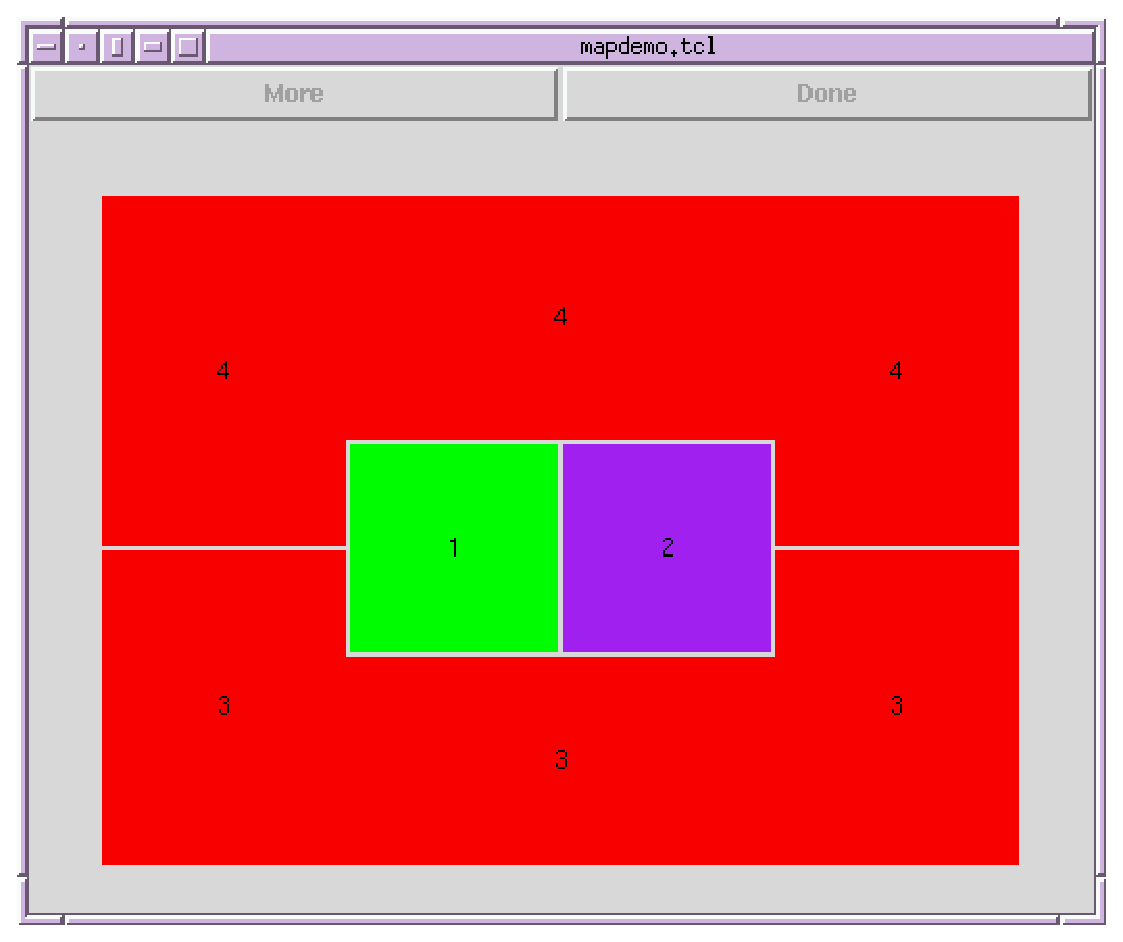
\includegraphics{mapdisplay2.ps}}}

\vspace{3mm}
{\bf Map Display of Program}
\end{center}

The countries are identified by numbers displayed within each country, and 
in this case, an incorrect colouring for the map is shown, because
countries 3 and 4 have the same colour. 

This program uses code from the map colouring demo program, and is
designed to use the GUI to display a map. Most of this is
not relevant to our debugging session, and although we will see some of this
code during the debugging, it is not necessary to understand it. 
You can think of this
debugging session as debugging someone else's code, not all of which
needs to be understood.

The program used here is included with your {\eclipse} distribution. You
should find it under the \texttt{doc/examples/tutorial} directory. You can
change to the \texttt{examples} directory in {\tkeclipse} using the
\menuopt{Change to example directory} option from the \menu{File} menu.

The final step in this debug tutorial is to edit the buggy program and
correct it. If you want to do this, you should copy the distributed version
of the program elsewhere so that you don't edit the original. You need to
copy the following files from \verb'examples/tutorial' to another directory:

\begin{quote}\begin{verbatim}
debugdemo.ecl  mapcolour.ecl mapdebugdemo.tcl buggy_data.map
\end{verbatim}\end{quote}

To load the program, start {\tkeclipse}. After start up, 
switch the working directory to
where you have the programs -- if you are using a UNIX system, and have
started {\tkeclipse} in the directory of the programs, you are already
there. Otherwise, go to the \menu{File} menu of {\tkeclipse}, and select
the \menuopt{Change directory} option. Use the directory browser to find
the directory containing your programs and select it. This will change your
working directory to the selected directory.

Next, compile \verb'debugdemo.ecl'. You can do this by selecting the
\menuopt{Compile} option from the \menu{File} menu (you can also compile
the file with the query \verb'[debugdemo]' from the query entry
window). 

\section{Running the Program}
To start the program, the query `colour' is run: type \verb'colour' 
into {\tkeclipse}'s query entry window, followed by the
return key. The program should run, and display the map to be coloured in a
window, which is then coloured, arriving at the
incorrect solution as shown previously. The program uses
the standard `generate-and-test' method, so you will see colour flashing in
the countries as the program tries different colours for them.

The map display has two buttons: pressing \button{More} will cause the program to
find an alternate way of colouring the map. Pressing \button{Done} will end the
program and return control to {\eclipse}. You can press \button{More} to get more
solutions and see that the program returns more solutions that colour
countries 3 and 4 to the same colour (along with some that are correct).

Press \button{Done} to finish the execution. We will now debug this program.

\section{Debugging the Program}


The main tool to debug a program is the {\bf tracer} tool. The tracer is
one of the development tools, all of which can be accessed from the \menuopt{Tools} menu of
{\tkeclipse}. Select \menuopt{Tracer} from the
menu as shown below, and a new window for the tracer tool should appear.

\begin{center}
\resizebox{0.5\textwidth}{!}{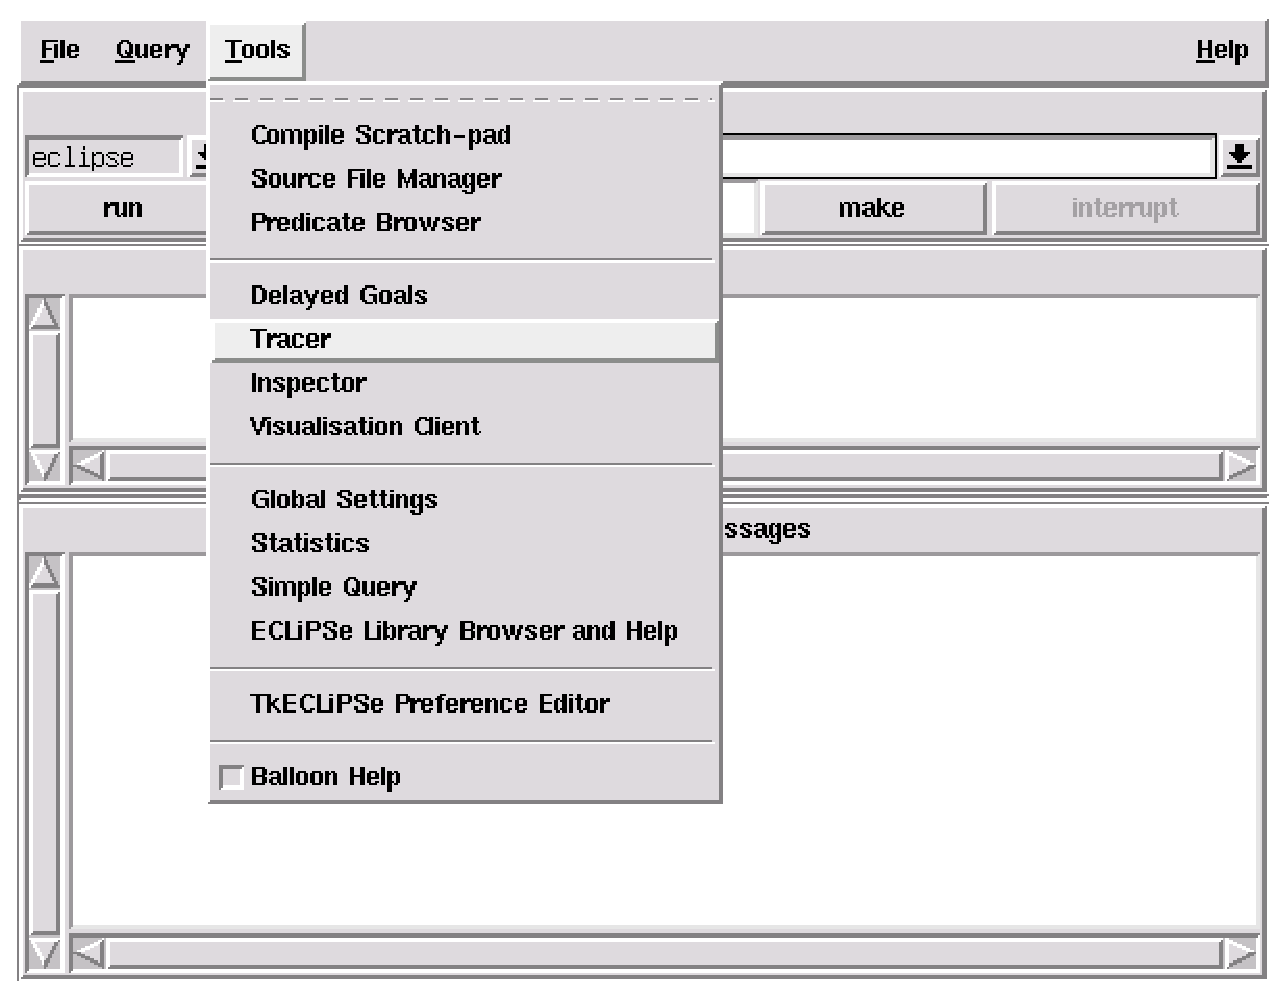
\includegraphics{tktoolsmenu.ps}}

\vspace{3mm}
{\bf Starting the Tracer Tool}
\end{center}
Run the query \verb'colour' again. To save you from typing in the query,
you can use the up-arrow on your keyboard to step back to a previous query.
Type return when  \verb'colour' appears in the query window again.

\begin{latexonly}
\begin{figure}
\begin{center}
\resizebox{0.35\textwidth}{!}{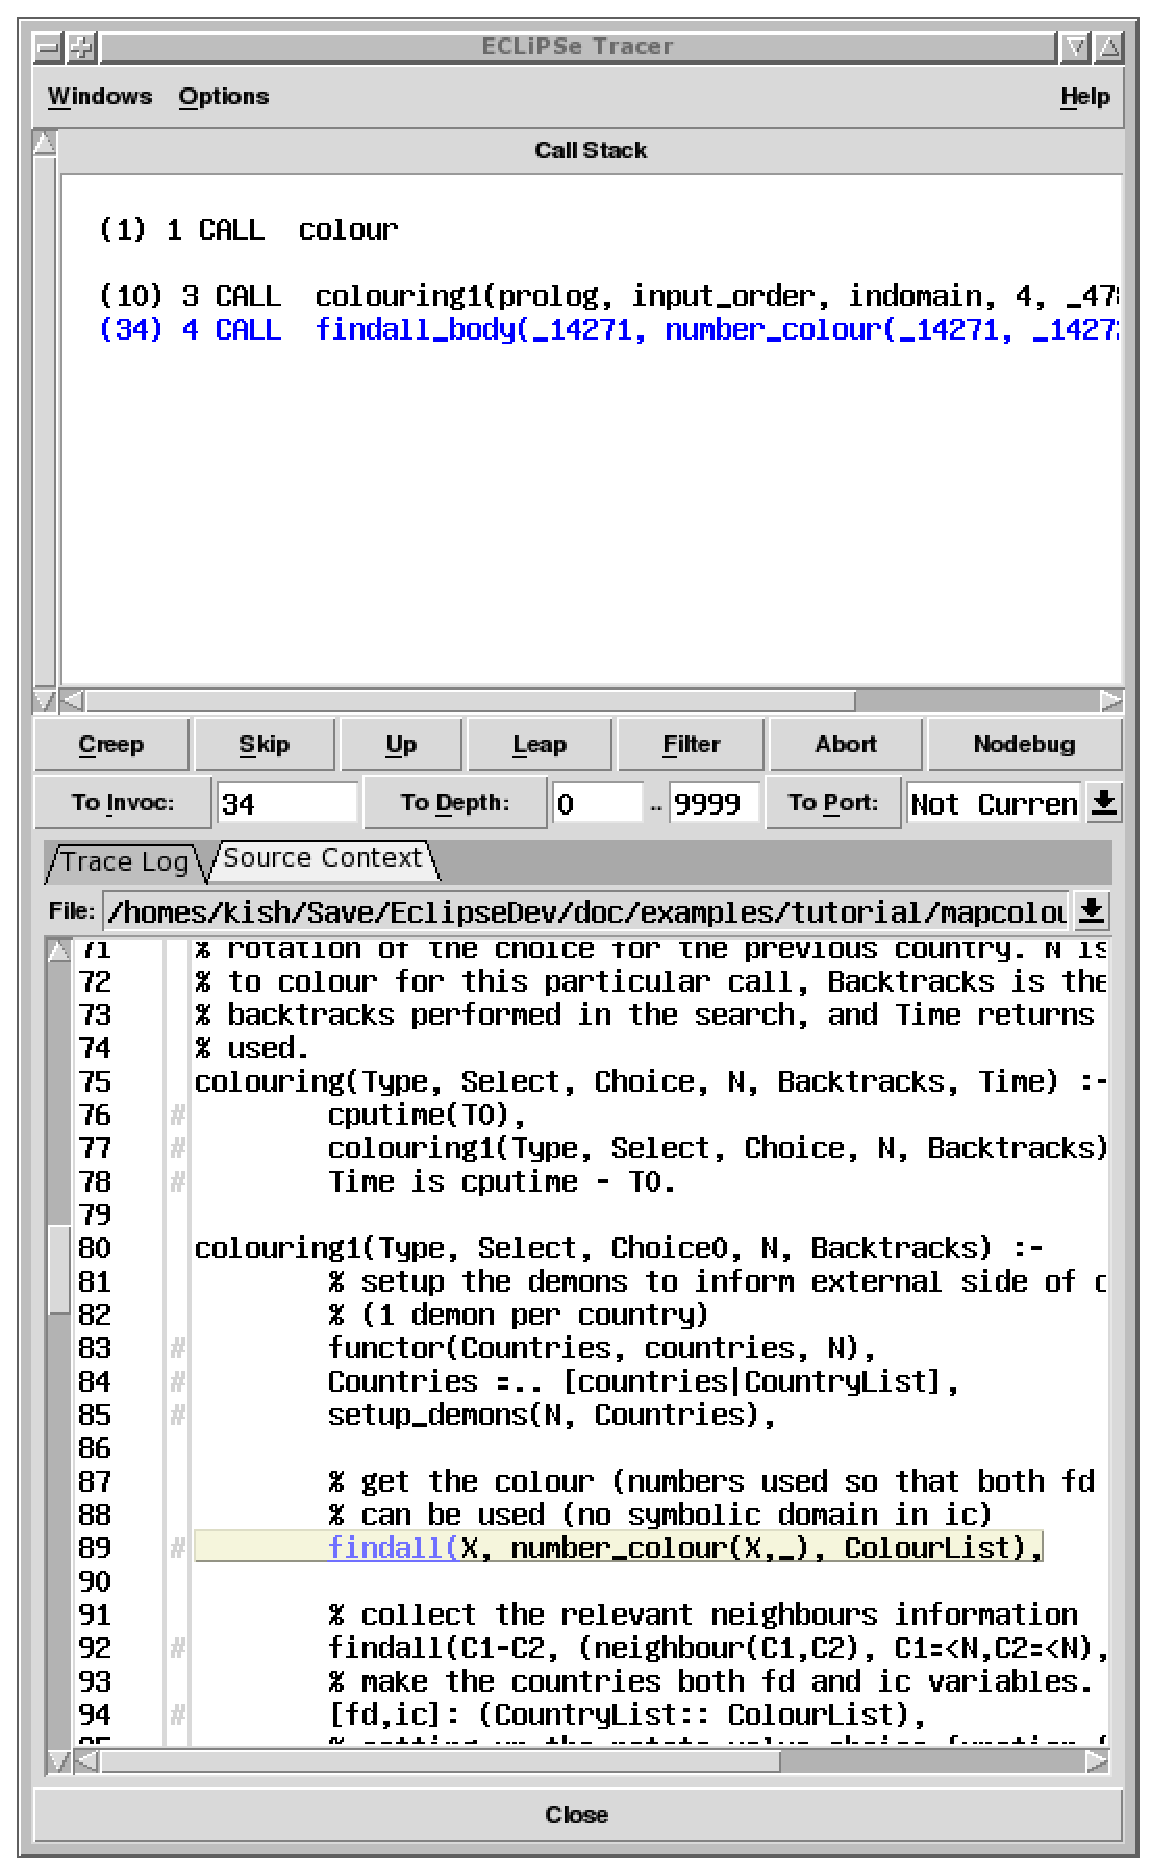
\includegraphics{tktracer.ps}}
\end{center}
\caption{The Tracer Tool}
\label{tktracer}
\end{figure}
\end{latexonly}

\begin{htmlonly}
\begin{figure}
\begin{center}
\resizebox{0.53\textwidth}{!}{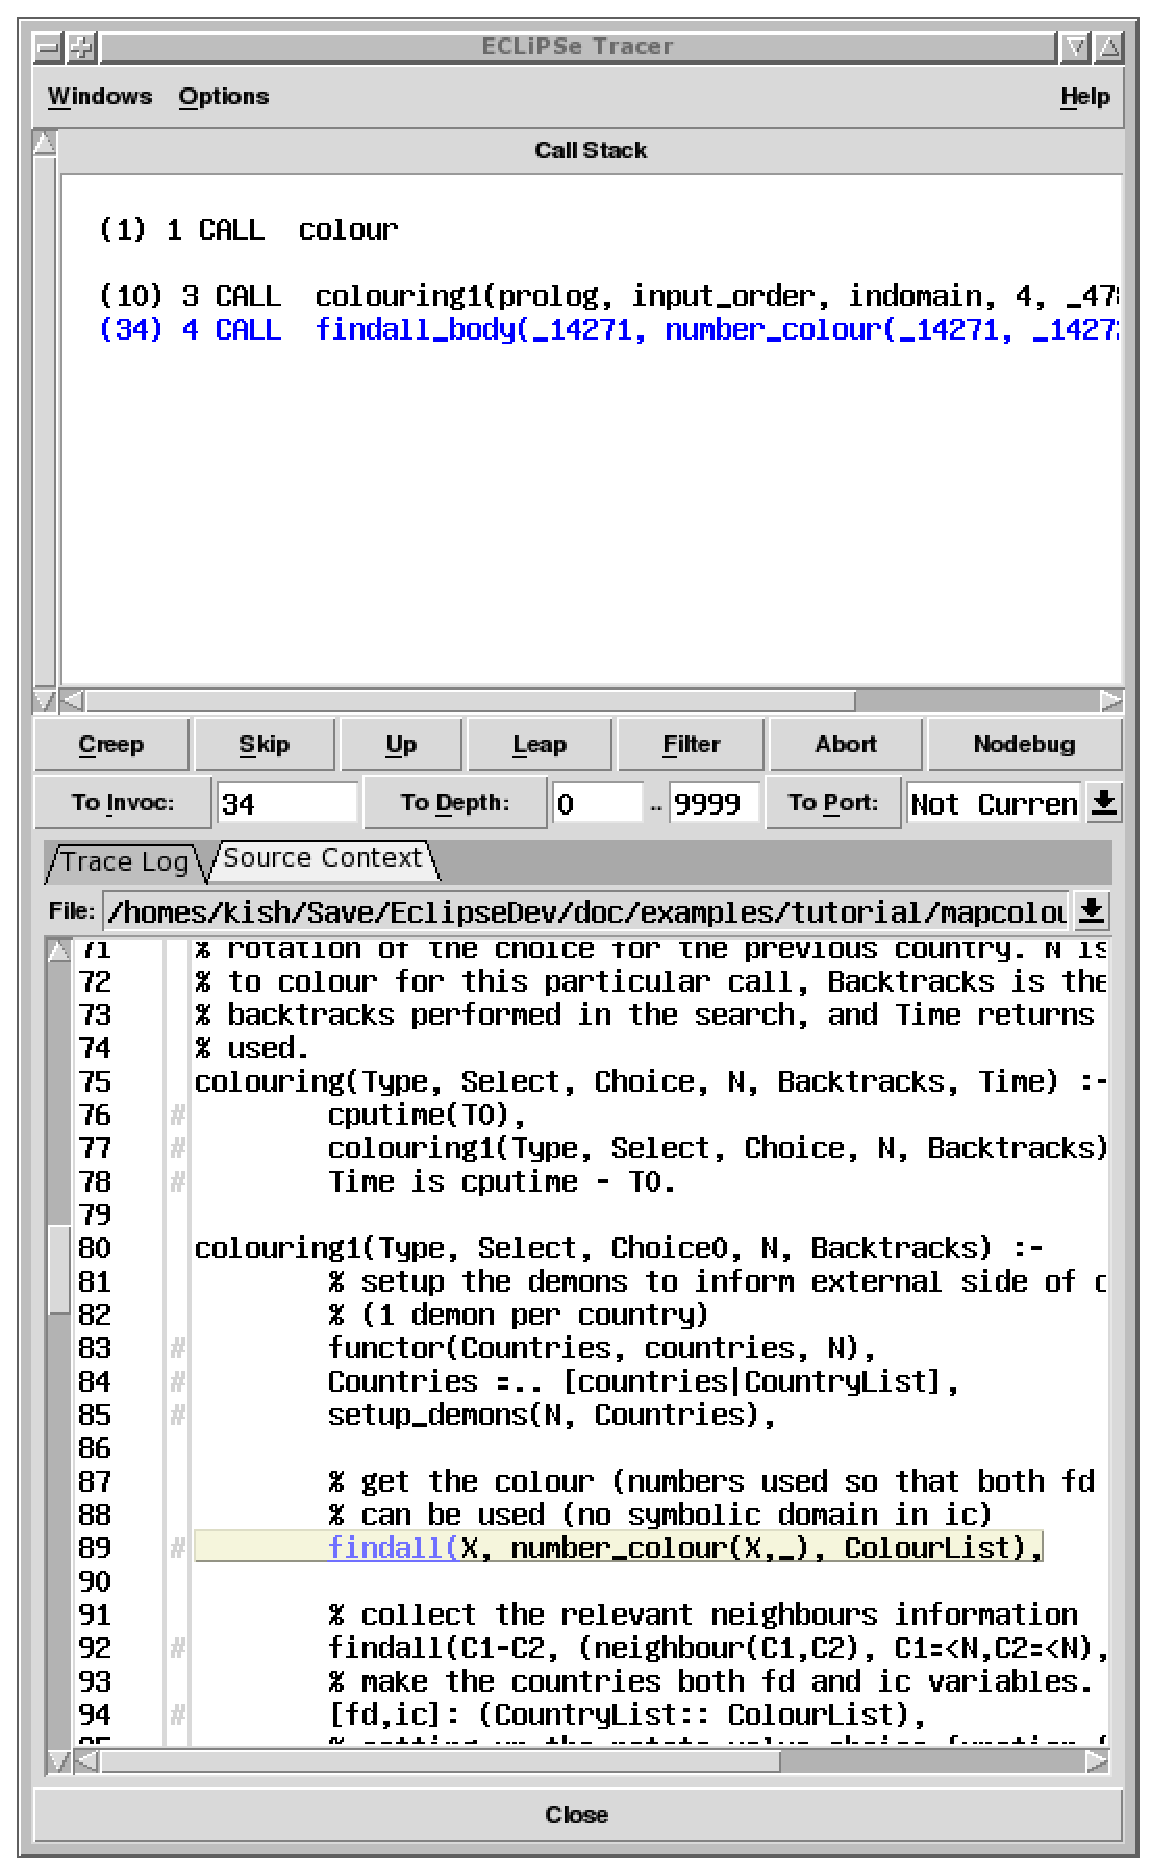
\includegraphics{tktracer.ps}}
\end{center}
\caption{The Tracer Tool}
\label{tktracer}
\end{figure}
\end{htmlonly}
\index{tracing program execution}
\index{tracer, development tool}

\quickref{Debugger Trace Line}{
\begin{small}
The trace lines displayed by the tracer has the following:
\begin{code}

 +(22) 14 *EXIT<3>  inform_colour(1, 1)

 1\quad2\quad\enspace3 4\quad\enspace5 6\qquad\qquad7

\end{code}
\begin{enumerate}
\item A '+' displayed here shows that the procedure has a spy point
  set. For a CALL port, a '\#' could be displayed in this position, which
  shows a breakpoint is set for the call.
\item The invocation number of this goal, which uniquely
  identifies it. The `To Invoc:' button can be used to jump to the next port with
  the specified invocation number. 
\item The depth of the goal, i.e. the number of its ancestors.
The `To Depth:' button can be used to jump to the next port within the specified
depth range.
\item An asterisk before an EXIT means that this
procedure is nondeterministic and that it might be resatisfied.
\item The type of the port. The `To Port:' button can be used to
  select the type of port to jump to.
\item This only appears if the goal is executing at a different priority
  than 12, the normal priority. The number is
  the priority that the  goal is executed at. 
\item The goal is printed according to the current instantiations
of its variables.  
\end{enumerate}
\end{small}
}

The tracer tool traces the execution of the program, like the traditional
Prolog debugger, it stops at  `debug ports' of predicates that are
executed.
\See{See the Debugging chapter in the User Manual for more details on the
  model used in Prolog debuggers.}
At the start of tracing,
it is stopped at the call port of the query \verb'colour'. The buttons in
the middle of the tool are for debugger commands. Try pressing
\button{Creep} several times, and you should observe something similar to
Figure~\ref{tktracer}. Unlike the traditional debugger, the execution trace
is shown on two text windows: the bottom `Source Context' view, showing the
execution of the program in the context of the source, highlighting the
body goal that corresponds to the goal at the debug port; and the
top `Call Stack' window, showing the ancestors (`call stack') of the
current goal, which is updated at each debug port. The goals are
displayed with different colours: blue for a call port, green (success) for
an exit port. Red (failure) for a fail port. Note that in the call
stack, the ancestor goals are displayed in black: this indicates that the
goal is not `current', i.e.\ the bindings shown are as they were when the
goal was called, and not necessarily what they are now. We will show how
these bindings can be `refreshed' later on. Note that the bottom windowc
can ne switched between the source context view, and a more traditional
`Trace Log' view, which shows a log of the debugger ports much as a traditional Prolog debugger does.

To avoid stepping through the whole program, we will add a spy-point to a
predicate that may be causing the problem. Spy-points can be added in the
traditional way, using the \verb'spy/1' predicate. However, we can also use
the {\bf predicate browser} tool:  start the \menuopt{Predicate Browser} tool
from the \menu{Tools} menu of {\tkeclipse}. This tool allows you to observe
and change various properties of the predicates in your program.
A list of predicates are displayed
on the left hand side, and a list of properties on the right.
Currently the predicate list is showing all the predicates defined in our program (i.e.\ in
the \verb'eclipse' module). Looking at this list,
\verb'not_same_colour/3''s name suggests that
it checks that neighbouring countries do not have the same colour.
Select it by clicking on it, and now the right
hand side should display the properties of this predicate:

\begin{center}
\resizebox{0.55\textwidth}{!}{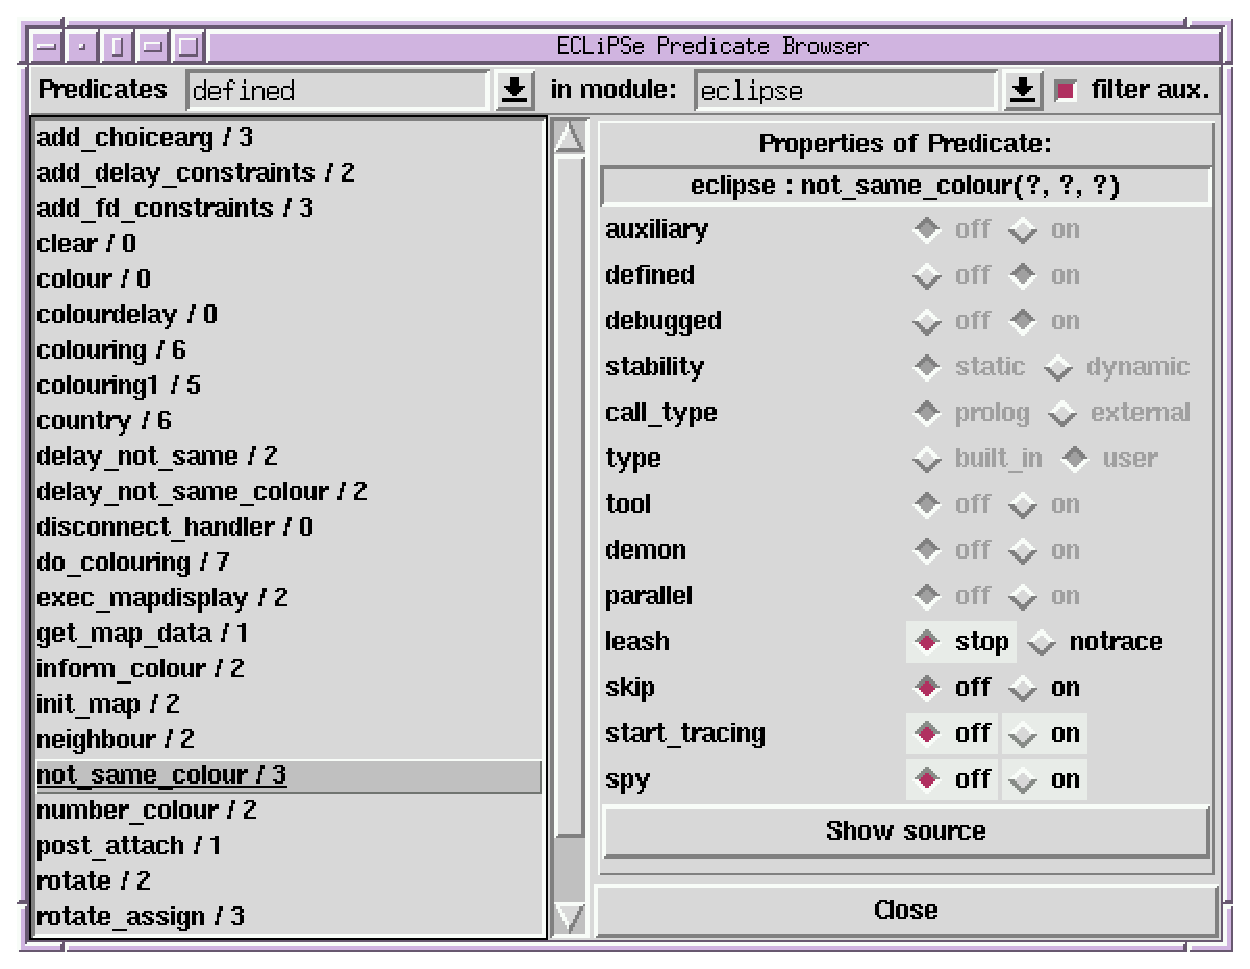
\includegraphics{tkpredbrowser.ps}}

\vspace{3mm}
{\bf The Predicate Browser Tool}
\end{center}
\index{predicate browser, development tool}

We can now view the source code for the predicate by clicking on the
\button{Show source} button, which will show the selected predicate's source in
the source context view. The code for the predicate is:

\begin{code}
not_same_colour(Solver, C1-C2, Countries) :-
      % get the colours for the countries C1 and C2
      arg(C1, Countries, Colour1),
      arg(C2, Countries, Colour2),
      % send constraint to either the fd or ic solver
      Solver: (Colour1 #\verb'\'= Colour2).
\end{code}

The code does indeed check that the countries \verb'C1' and \verb'C2' do
not have the same colour.

\Note{For our example program, the list is not very long, but some programs may
have many predicates, and it could be difficult to find the predicate you
want. The predicate list has a search facility: typing in part of the name
of the predicate in the predicate list will search for the predicate you
want. You can try typing in {\tt not_same_colour / 3} to see how this
works.}

The predicate browser allows us to change some of the properties of a predicate.
We can add a spy-point to the predicate by clicking on the radio button for
{\bf spy}: 

\begin{center}
\resizebox{0.27\textwidth}{!}{
\includegraphics{tkpredspyon.ps}}

\vspace{2mm}
{\bf Setting Spy Property to On}
\end{center}

With {\tkeclipse}, we can do more than just place a spy point on a
predicate: we can specify further conditions for when the tracer should
stop at a spy point, using the filter tool. 

Start the filter tool by selecting \menuopt{Configure filter} from the \menu{Options} menu of the tracer
tool:

\begin{center}
\resizebox{0.4\textwidth}{!}{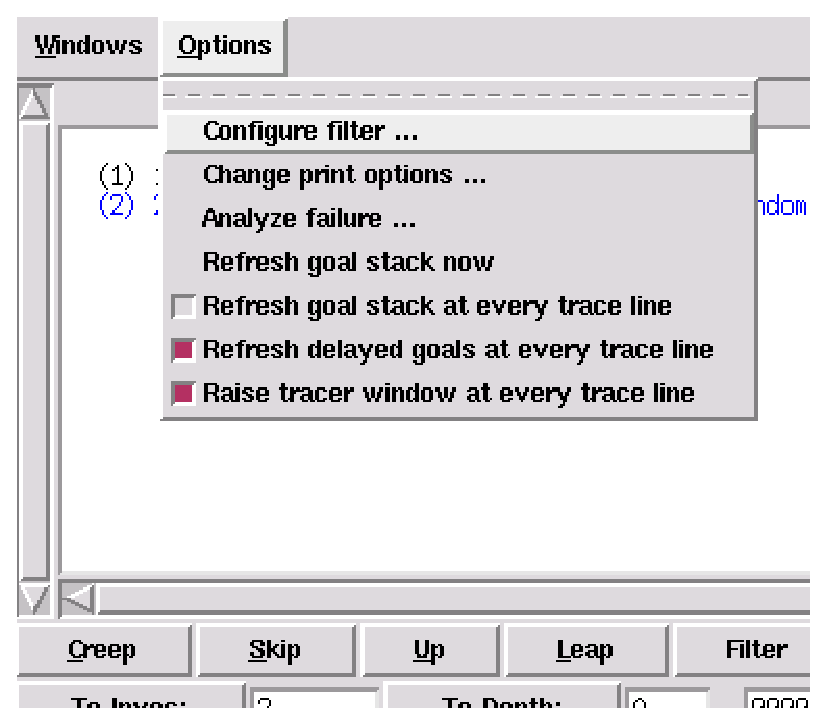
\includegraphics{tktraceroptions.ps}}

\vspace{3mm}
{\bf Starting the Filter Tool from the Tracer}
\end{center}

\begin{figure}
\begin{center}
\resizebox{0.5\textwidth}{!}{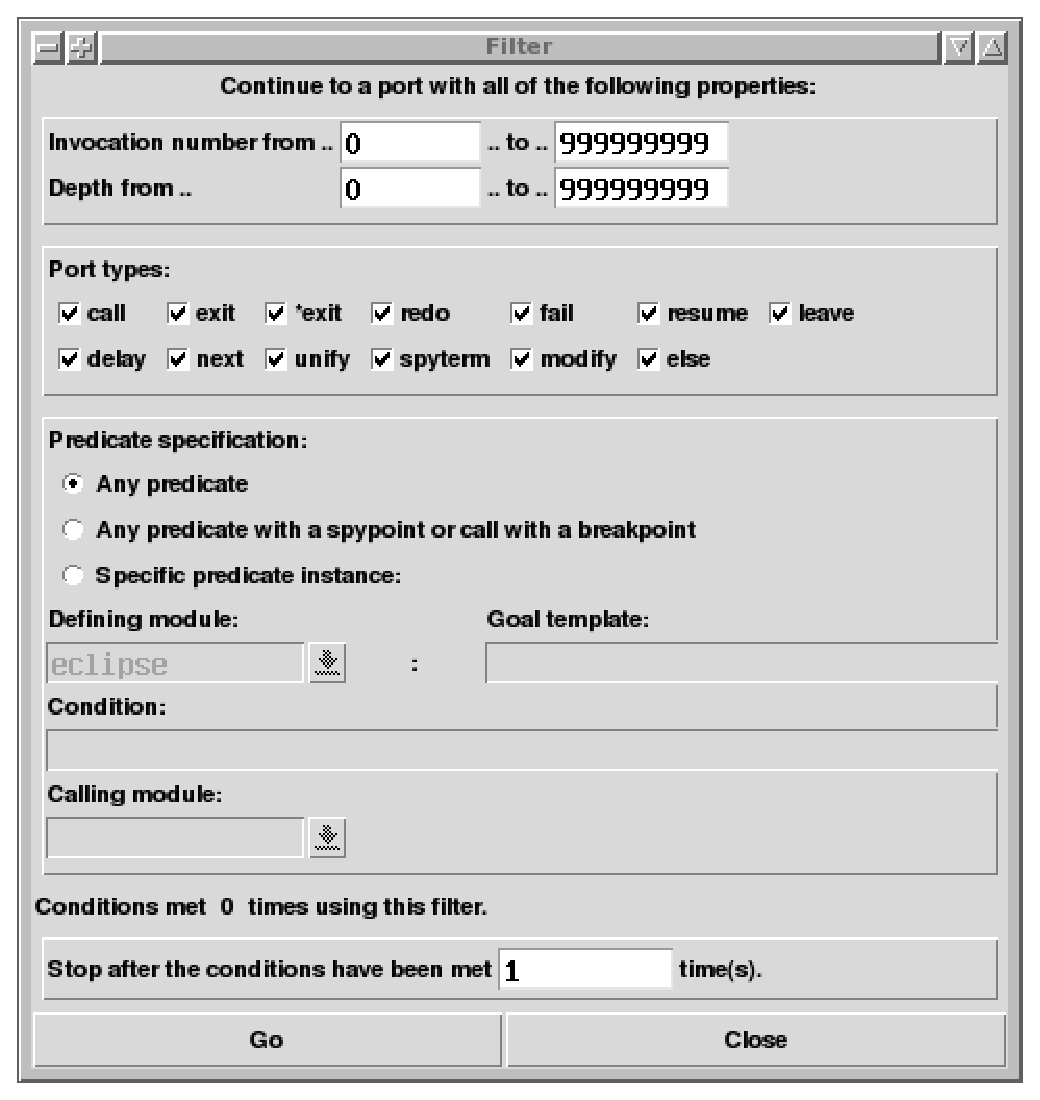
\includegraphics{tkfilter.ps}}
\end{center}
\caption{The Tracer Filter Tool}
\label{tkfilter}
\end{figure}

The filter tool opens in a new window, as shown in
Figure~\ref{tkfilter}. This tool allows us to specify a `filter' for the
debug ports so that the tracer will only stop at a port with the properties
specified by the tool. In our case, we want to see \verb'not_same_colour/3'
only when countries 3 and 4 are involved. This can be done 
with the ``Predicate specification'' facility, enabled by the
\button{Specific predicate instance:} radio button. Pressing this button
will allow us to specify a condition in Prolog syntax which will be
checked at each debug port. For our purpose, we enter the following:

\begin{center}
\resizebox{0.55\textwidth}{!}{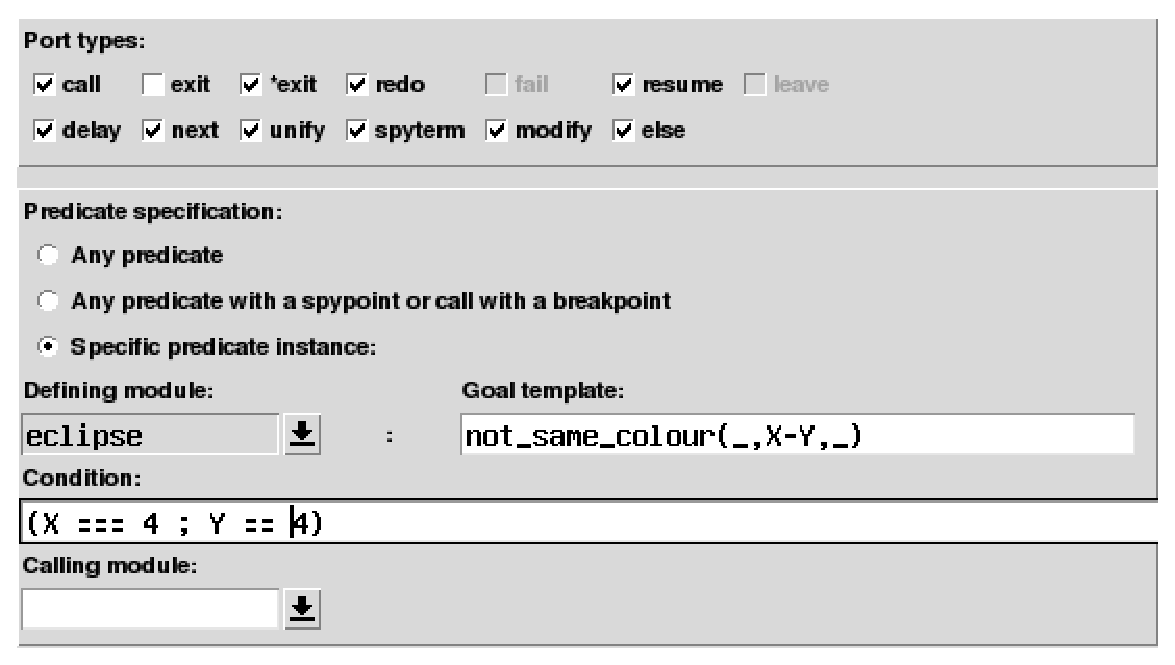
\includegraphics{tkfiltercond.ps}}

\vspace{3mm}
{\bf Setting Conditions for Specific Predicate Instances}
\end{center}

\index{conditional spying}
\index{tracer filter, development tool}
This specifies that the filter should stop at a \verb'not_same_colour/3'
goal, when one of the countries in the pair \verb'X-Y' is country 4: the {\bf
Goal template} is used to specify the template the debug port goal should
match, and the {\bf Condition:} can be any {\eclipse} goal, perhaps with variables
from the {\bf Goal template}, as in our case. The test is done by unifying
the goal with the template, and then executing the condition. Note that any
bindings are undone after the test. 

Note that we have also deselected the \button{exit} port in the filter
condition. You can do this by clicking on the \button{exit} radio
button. This means that the tracer does not stop at any exit port.

Press \button{Go} on the filter tool to start the tracer running with the
filter. You can also press the \button{Filter} command button on the tracer
to do the same thing.
We see that the tracer has jumped to a \verb'not_same_colour/3' goal
involving country 4 as expected. However, there is a gap in the call stack
as we skipped over the tracing of some ancestor goals. We can see these
goals by {\bf refreshing} the goal stack. This can be done by pressing and
holding down the right mouse button while the mouse cursor is over a goal
in the call stack, which will popup a menu for the goal:

\begin{center}
\resizebox{0.55\textwidth}{!}{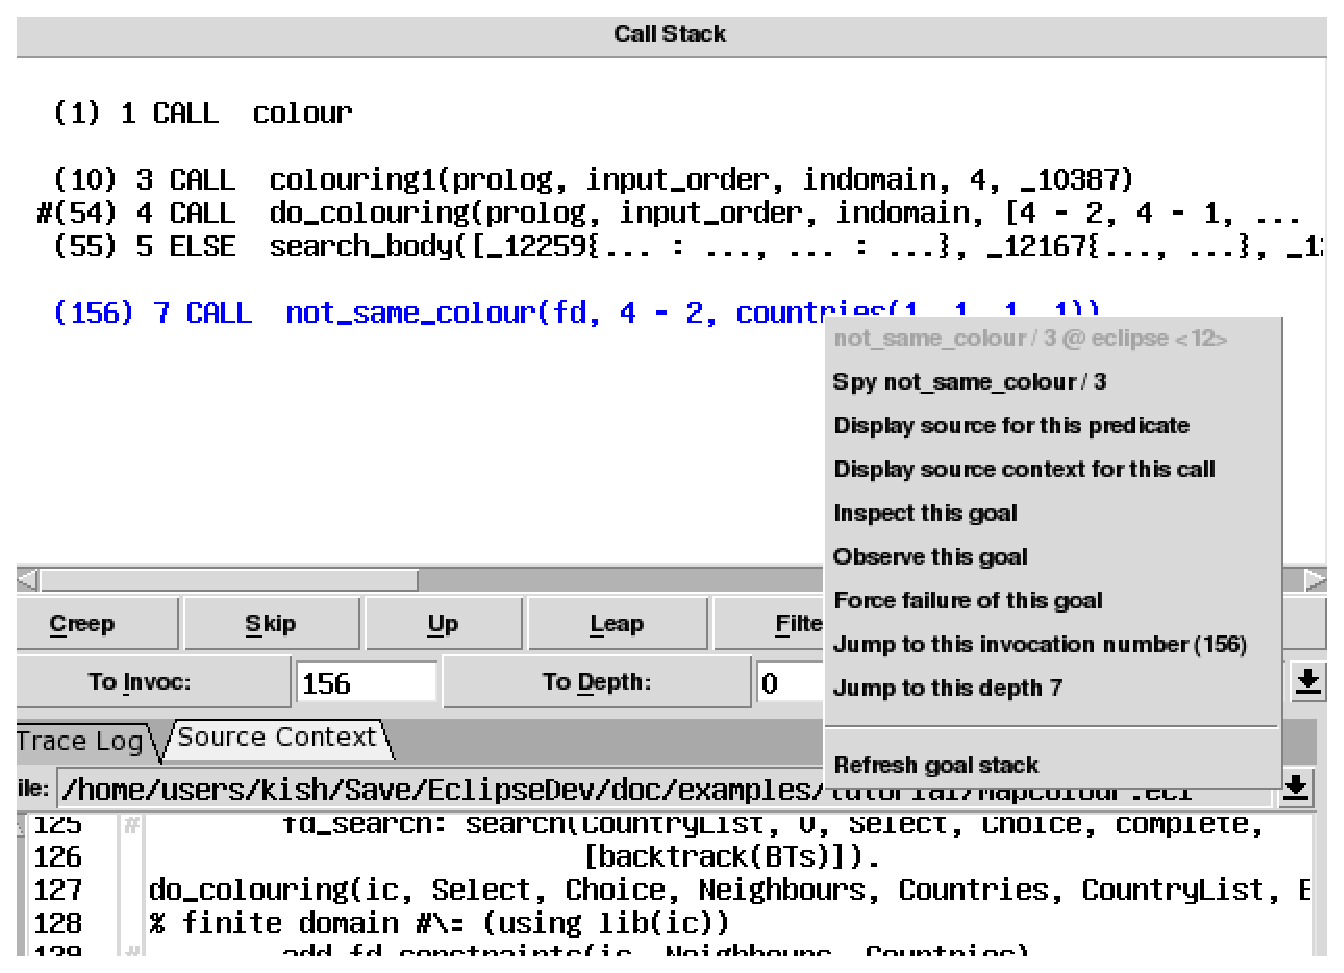
\includegraphics{tktracerpopup.ps}}

\vspace{3mm}
{\bf Popup Menu for a Goal in Tracer's Call Stack}
\end{center}

In this case, we have opened the menu over \verb'not_same_colour/3', and the
options are for this goal. Various options are available, but for now we
choose the \menuopt{Refresh goal stack} option. This will result in the
following goal stack display:

\begin{center}
\resizebox{0.6\textwidth}{!}{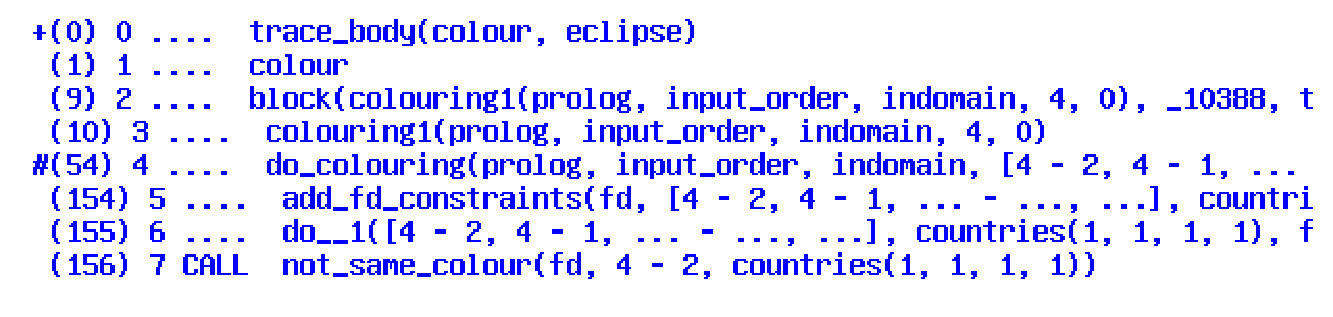
\includegraphics{tkrefreshedgs.ps}}

{\bf Refreshed Call Stack}
\end{center}

Notice that the colour of the goals in the goal stack are now all blue,
indicating that the bindings shown are current. 

Press \button{Filter} on the tracer several times to jump to other ports
involving country 4. You will see that none of them involve countries 3 and
4. So perhaps countries 3 and 4 are not checked by
\verb'not_same_colour/3', i.e.\ \verb'3-4' or \verb'4-3' are never passed
to \verb'not_same_colour/3'. Looking at the call stack, we can see that the
country pair in \verb'not_same_colour/3' seem to appear as an element in a
list of country pairs, as far back as \verb'colouring(...)'. Unfortunately,
the debugger does not display the whole list. We see something like:

\begin{center}
\verb'do_colouring(prolog, input_order, indomain, [4 - 2, 4 - 1, ... '
\end{center} 
\noindent
due to the `print depth' feature, which shortens the printing of large
terms. We can examine the whole list by using the inspector to examine the
goal. To do this, we double click on the \verb'do_colouring(...)' goal
to `open' it for inspection.

This will launch the Inspector tool on the \verb'do_colouring' goal. The
inspector displays the term in a hierarchical fashion as a tree, which
allows us to navigate the term. The initial display is shown on the left
panel below. We are interested in examining the full list. We can look at
this list by double clicking on it to expand the node, which results in the
display in the right panel below. You may need to scroll
down to see the whole list:

\begin{center}
\parbox{0.49\textwidth}{\resizebox{0.48\textwidth}{!}{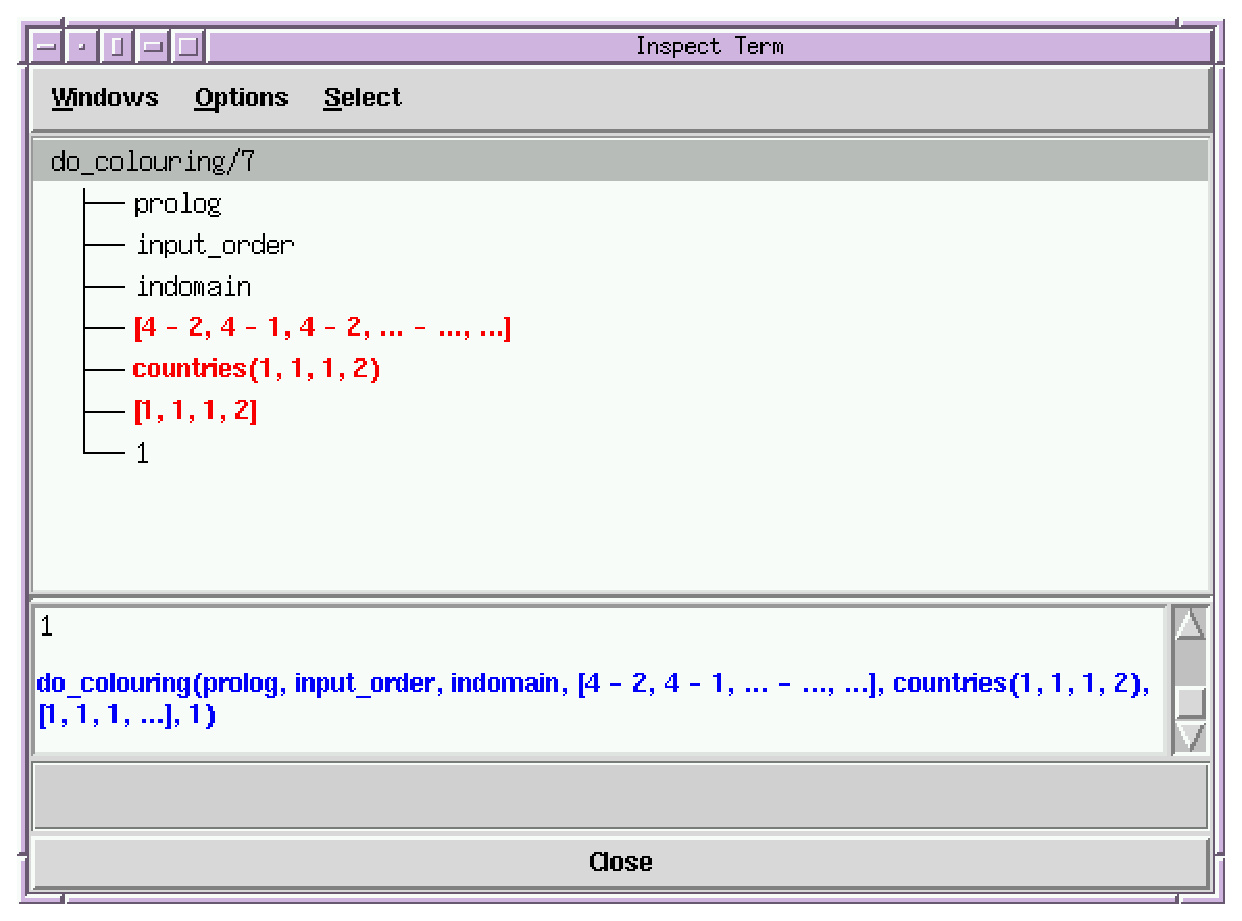
\includegraphics{tkinspect.ps}}}
\parbox{0.49\textwidth}{\resizebox{0.48\textwidth}{!}{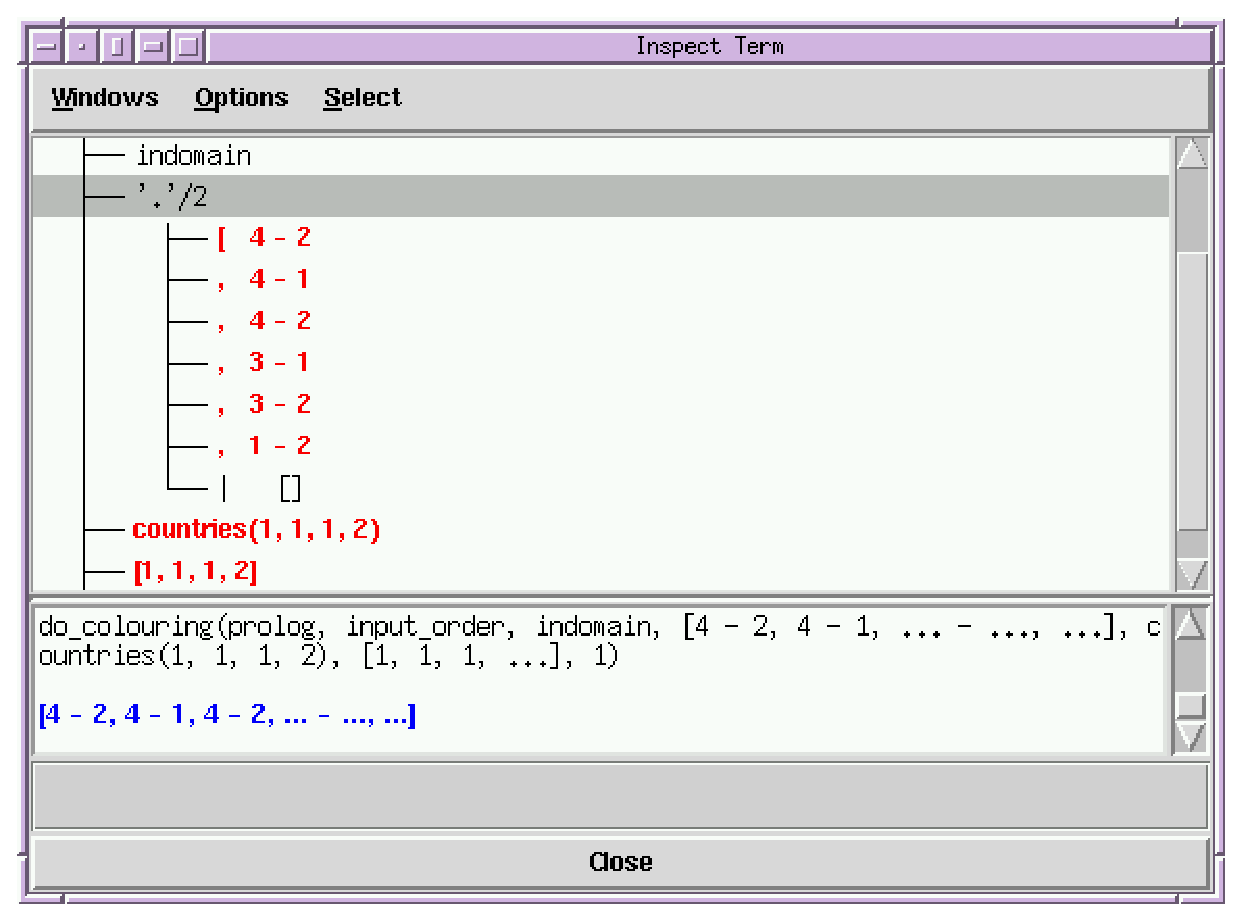
\includegraphics{tkinspect2.ps}}}

\vspace{3mm}
{\bf Using the Inspector}
\end{center}

\index{term inspector, development tool}
\index{inspecting terms}
The inspector shows that this list does not contain the pair \verb'4-3' or
\verb'3-4', which should be there so that \verb'not_same_colour'
can check that these two countries  are not assigned the same colour.

\begin{sloppypar}
The inspector tool is modal -- when it is open, the rest of {\tkeclipse} is
inaccessible. Close the Inspector by clicking on its
\button{Close} button, go back to the tracer, and see where the country
pair list comes from. It
first appears in 
the ancestor goals \verb'do_colouring(prolog,...)', as the next parent
\verb'colouring(prolog,...)' does not have this list. So the list
is created in a body goal of \verb'colouring(...)' before \verb'do_colouring(...)' is
called. We can look at the source of \verb'colouring(...)'  to see how this
list is created. To do this, we can
select \menuopt{Display source} option from the popup menu for the
\verb'colouring(...)' goal:
\end{sloppypar}
 
\begin{center}
\resizebox{0.55\textwidth}{!}{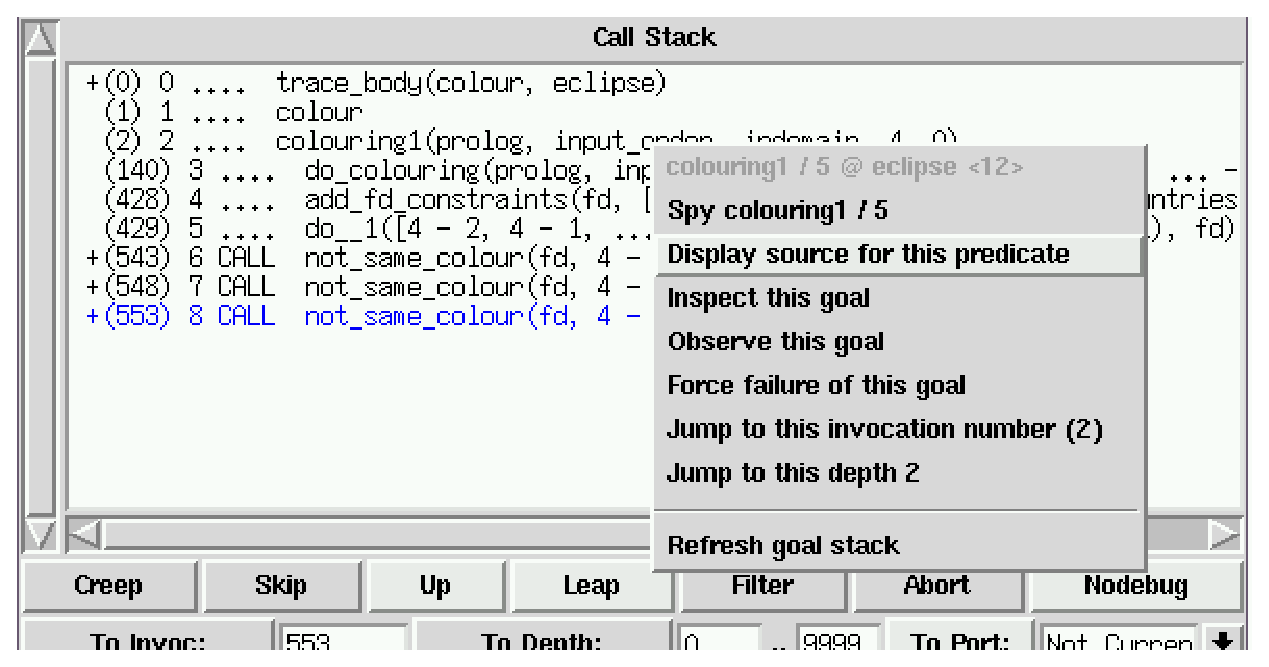
\includegraphics{tktracerpopup2.ps}}

\vspace{3mm}
{\bf Displaying Source for a Goal in the Call Stack}
\end{center}

The code for this predicate is quite long, but for our purposes we are only
interested in the country-pair list that is passed to \verb'do_colouring':

\begin{code}
colouring1(Type, Select, Choice0, N, Backtracks) :-
        ....
        findall(C1-C2, (neighbour(C1,C2), C1=<N,C2=<N), Neighbours),
        ....
        do_colouring(Type, Select, Choice, Neighbours, Countries,
                     CountryList, Backtracks), 
        ....
\end{code}

Looking at this source and the Call stack goal, we can see that the country
pair list is constructed from \verb'neighbour/2' calls. Let's look at the
source for \verb'neighbour/2'. We can do this from the predicate browser, by
selecting \verb'neighbour/2' and pushing the \button{Show source} button. We see
the following:

\begin{code}
neighbour / 2 in file buggy_data.map, line 2:
%neighbour(4, 3).
neighbour(4, 2).
neighbour(4, 1).
neighbour(4, 2).
neighbour(3, 1).
neighbour(3, 2).
neighbour(1, 2).
\end{code}


So \verb'neighbour(4,3)' was indeed missing (it is commented out).
Another way to check \verb'neighbour/2', without looking at the source,
would be using the
Simple Query tool. This tool is again started from {\tkeclipse}'s
\menu{Tools} menu. It can be used to send simple queries to {\eclipse},
even while another query is being executed (as we are here, executing the
\verb'colour' query). We can use this tool to check if \verb'neighbour(4,3)'
or \verb'neighbour(3,4)' are defined or not:

\begin{center}
\resizebox{0.55\textwidth}{!}{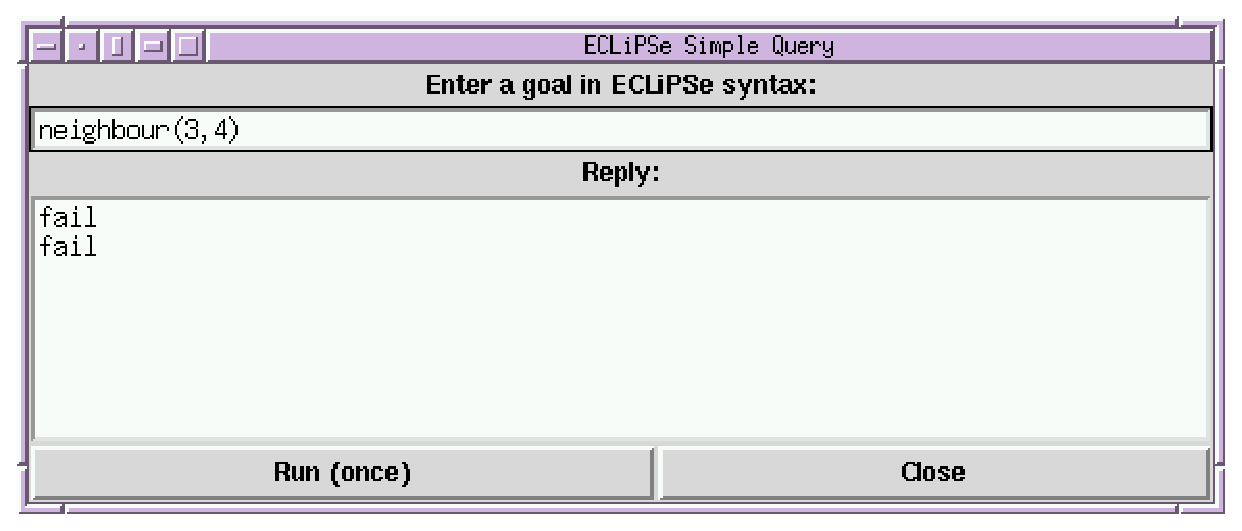
\includegraphics{tkquery.ps}}

\vspace{3mm}
{\bf The Simple Query Tool}
\end{center}

To send a query, simply type it in the entry window and press return, and
the reply will be sent to the reply window. In the example above, we have
tried \verb'neighbour(4,3)', followed by \verb'neighbour(3,4)', and
both failed, indicating that there is no neighbour relationship defined
between countries 3 and 4.

\begin{sloppypar}
 We can fix the program by editing
the file \verb'buggy_data.map' and adding the neighbour(4, 3) line back.
TkECLiPSe does not provide an integrated editor itself, so you need to use
some external editor, such as emacs, vi, or wordpad to edit the program. 
You can tell \eclipse which editor you want to use, so that you can invoke
the editor from within \eclipse. For example, from the source context view
window of the tracer, you can invoke an editor to edit the file being
\begin{figure}
\begin{center}
\resizebox{0.3\textwidth}{!}{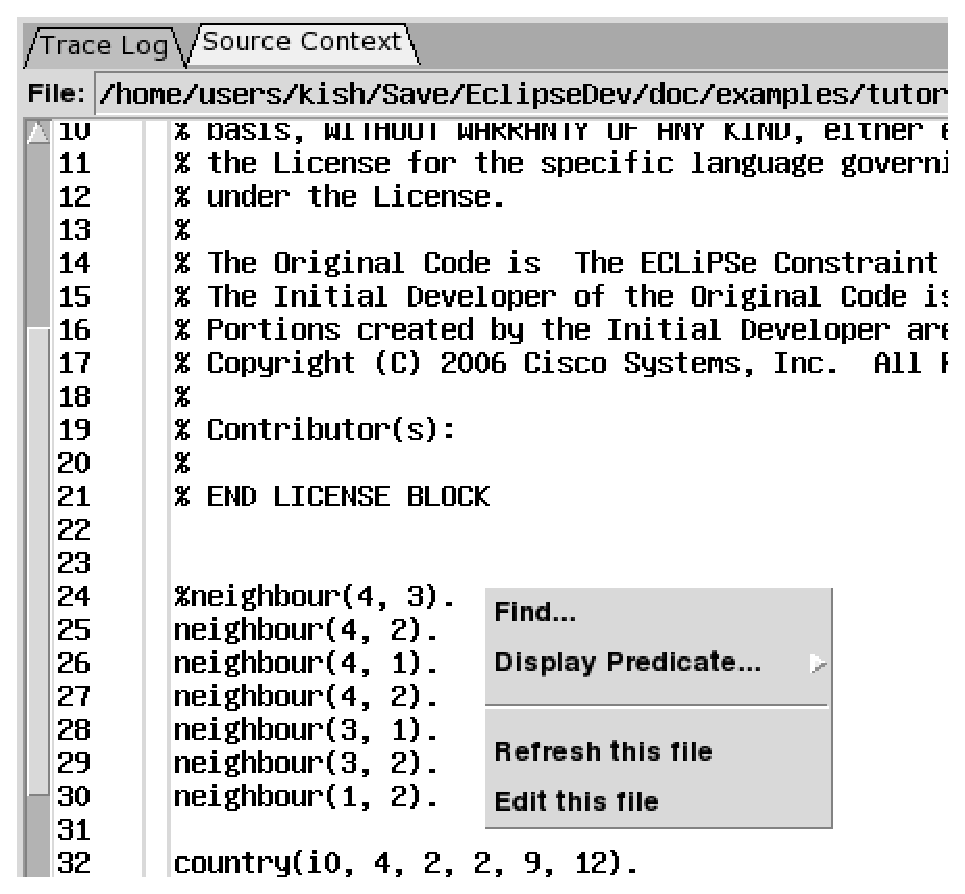
\includegraphics{tksoucontext.ps}}
\end{center}
\caption{Invoking an editor}
\label{tkeditor}
\end{figure}
displayed. Holding down your right mouse button in the source context
window will popup a menu, as shown in figure~\ref{tkeditor}. Select ``Edit
this file'' option will invoke your specified editor to edit the file, and if
possible, the file will be opened showing the line where your mouse pointer
was when you popup the menu (line 24 in this example).

\Note{
You can specify an editor to use with \eclipse using the Tkpreference
editor tool from the Tools menu. Fill in the entry for ``Text editor to use''
with the editor you want to use -- this should be the command that you will
type in a command line to invoke your editor. In addition, if your editor
supports it, you can fill in
the ``Editor's command line option to start at a specific line'' with the
command line option that will cause the editor to open the file at a
certain line.
}

To run the corrected program, we first end our current debugging session by
closing the tracer window. You can see from the map display that the
execution continues until a solution is produced. 
Pressing \button{Done} on the map display will return control to
{\eclipse}. Alternatively, if continuing the execution is undesirable,  press the \button{Abort} command button in
the tracer, which would abort the execution.
\end{sloppypar}

Once we have made the correction to the program and saved it,
we compile it by pressing the
\button{Make} button on {\tkeclipse}. This recompiles any files that
have been updated since {\eclipse} last compiled the file. 

Running the program again will show that the bug is indeed fixed.


\quickref{Mouse Button Operations on Objects}{
In {\tkeclipse}, you can usually perform these operations on an object
while the mouse cursor is over it:

\begin{description}
\item[left-click] selects the object. 
\item[double (left)-click] `opens' the object. This can mean expanding it
(e.g. in the inspector), or calling the inspector on it (e.g.\ on a goal in
the call stack), or showing the source for a goal (e.g. in the source
context view).
\item[Right-click and hold]  Opens a menu which gives
further option/information on the object.
\end{description}
Right-mouse button functionality are alternatively available through the
left-mouse button with the control key pressed.
}

\quickref{Available Development tools}{
{\small
\begin{description}
\item[Compile scratch pad] allow simple programs to be written and
compiled. Equivalent to {\tt [user]} in command line {\eclipse}.
\item[Source file manager] manage source files for this {\eclipse} session.
\item[Predicate browser]  view/change properties of predicates.
\item[Delayed goals] view delayed goals.
\item[Tracer] debugger for {\eclipse} programs.
\item[Inspector] term inspector. Useful for viewing large terms.
\item[Visualisation client] start a visualisation client.
\item[Global settings] view/change global {\eclipse} settings.
\item[Statistics] show statistics. Information is updated dynamically.
\item[Simple query] send simple queries to {\eclipse}.
\item[Library browser and help] interface to {\eclipse} documentation.
\item[TkECLiPSe preference editor] view/change {\tkeclipse} settings. 
\end{description}
}}

\section{Summary}
\subsection{{\tkeclipse} toplevel}
\index{toplevel}
\resizebox{0.8\textwidth}{!}{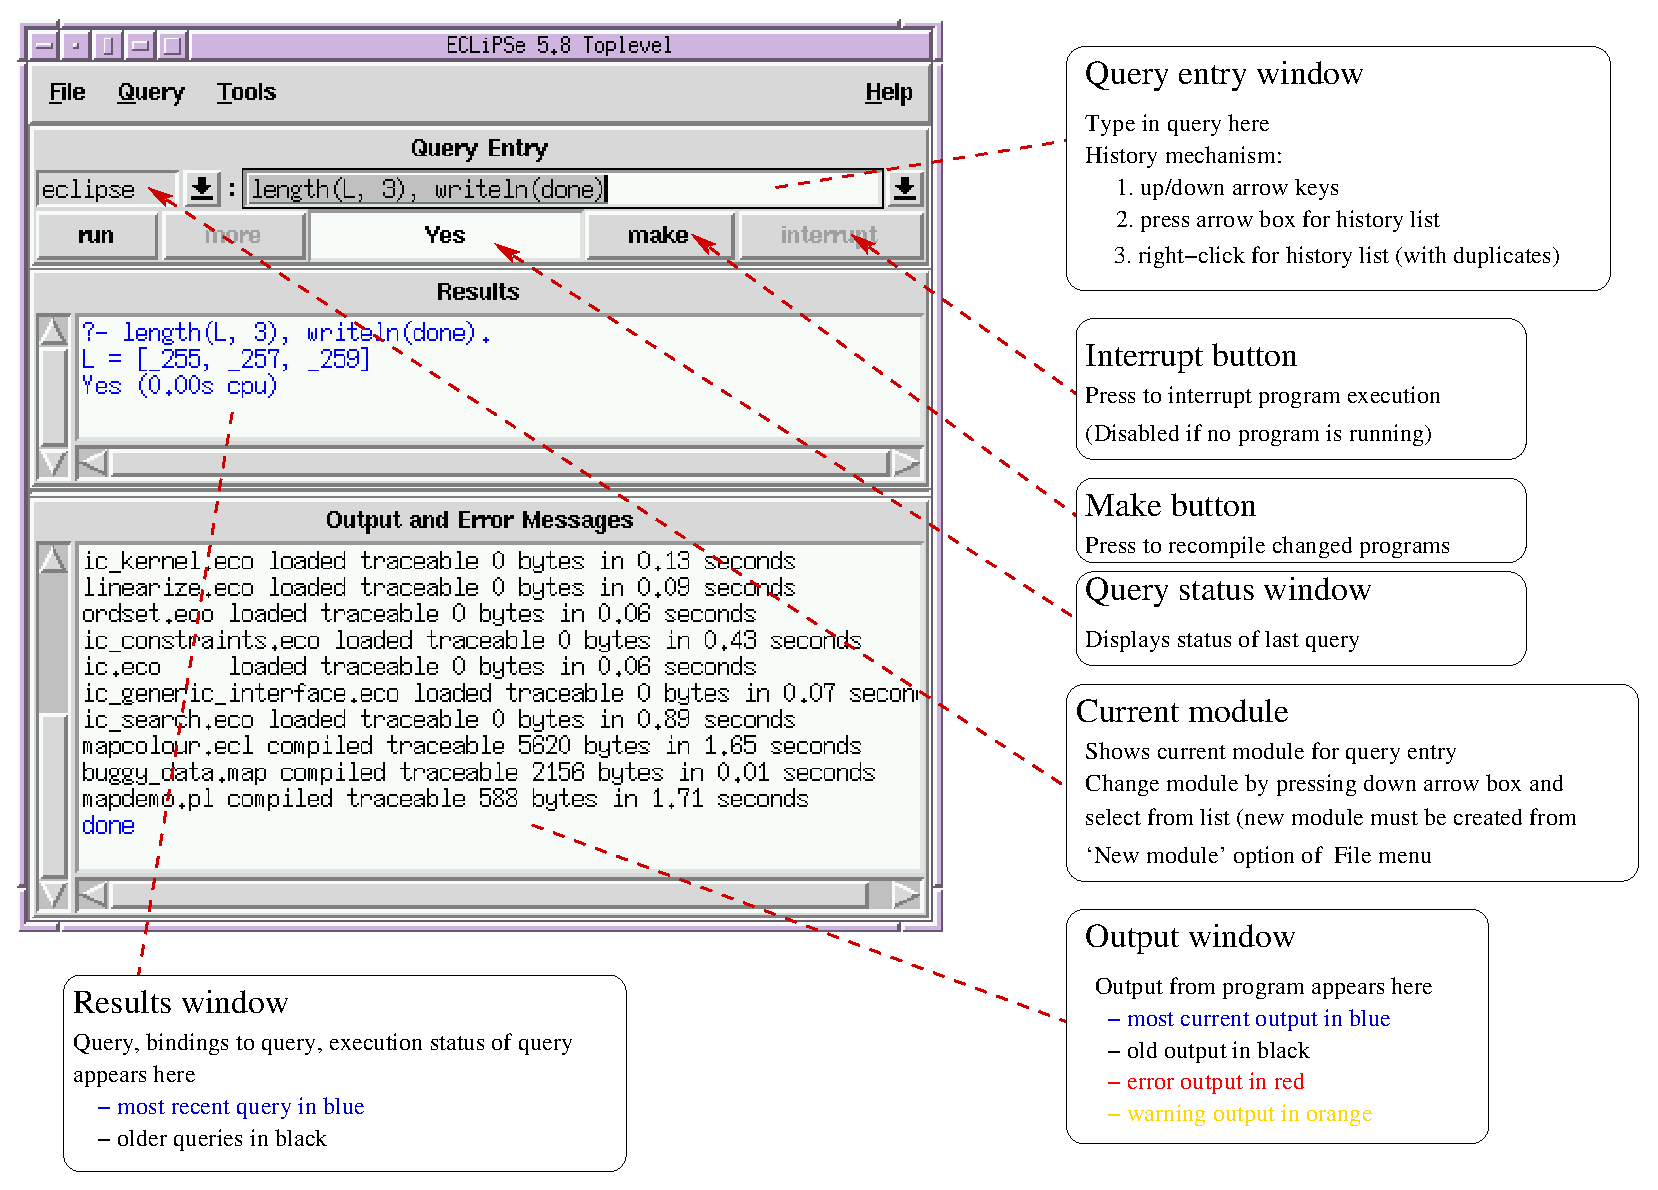
\includegraphics{tktopann.eps}}

\subsection{Predicate Browser} 
\index{predicate browser, development tool}
\resizebox{0.8\textwidth}{!}{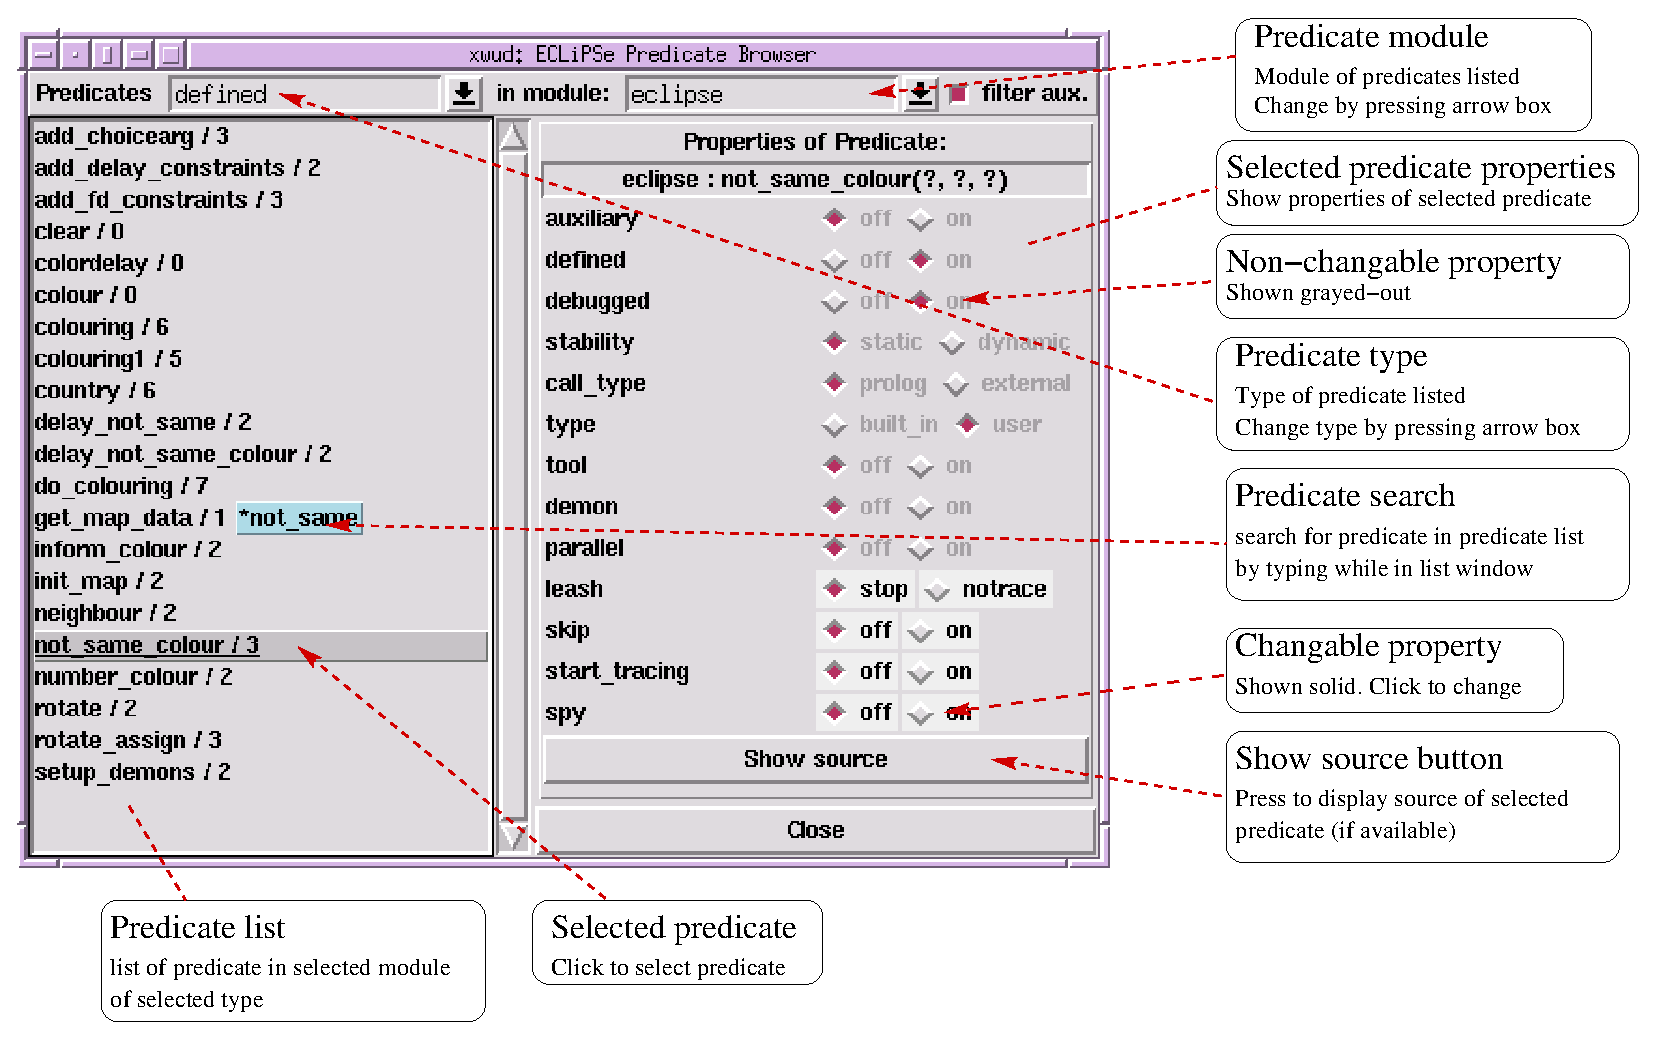
\includegraphics{tkpredann.eps}}

\subsection{Delayed Goals Viewer}
\index{delayed goals viewer, development tool}

\resizebox{0.7\textwidth}{!}{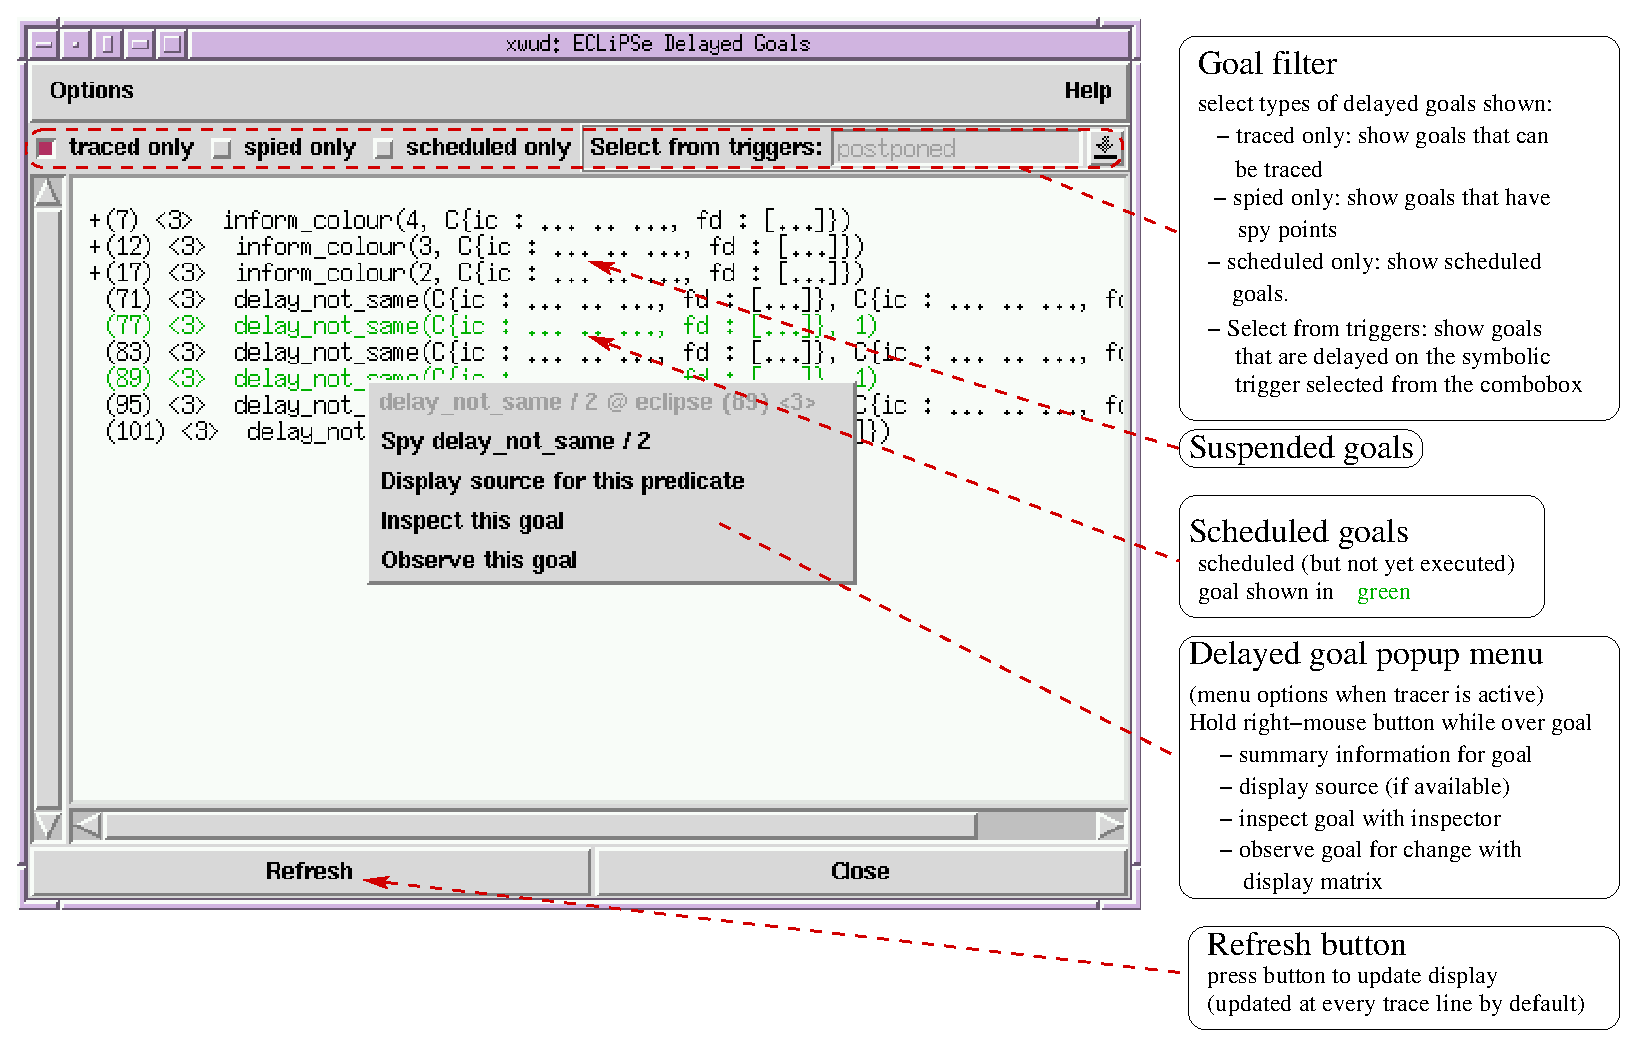
\includegraphics{tkdelayedann.eps}}
\subsection{Tracer}
\index{tracer, development tool}
\resizebox{0.75\textwidth}{!}{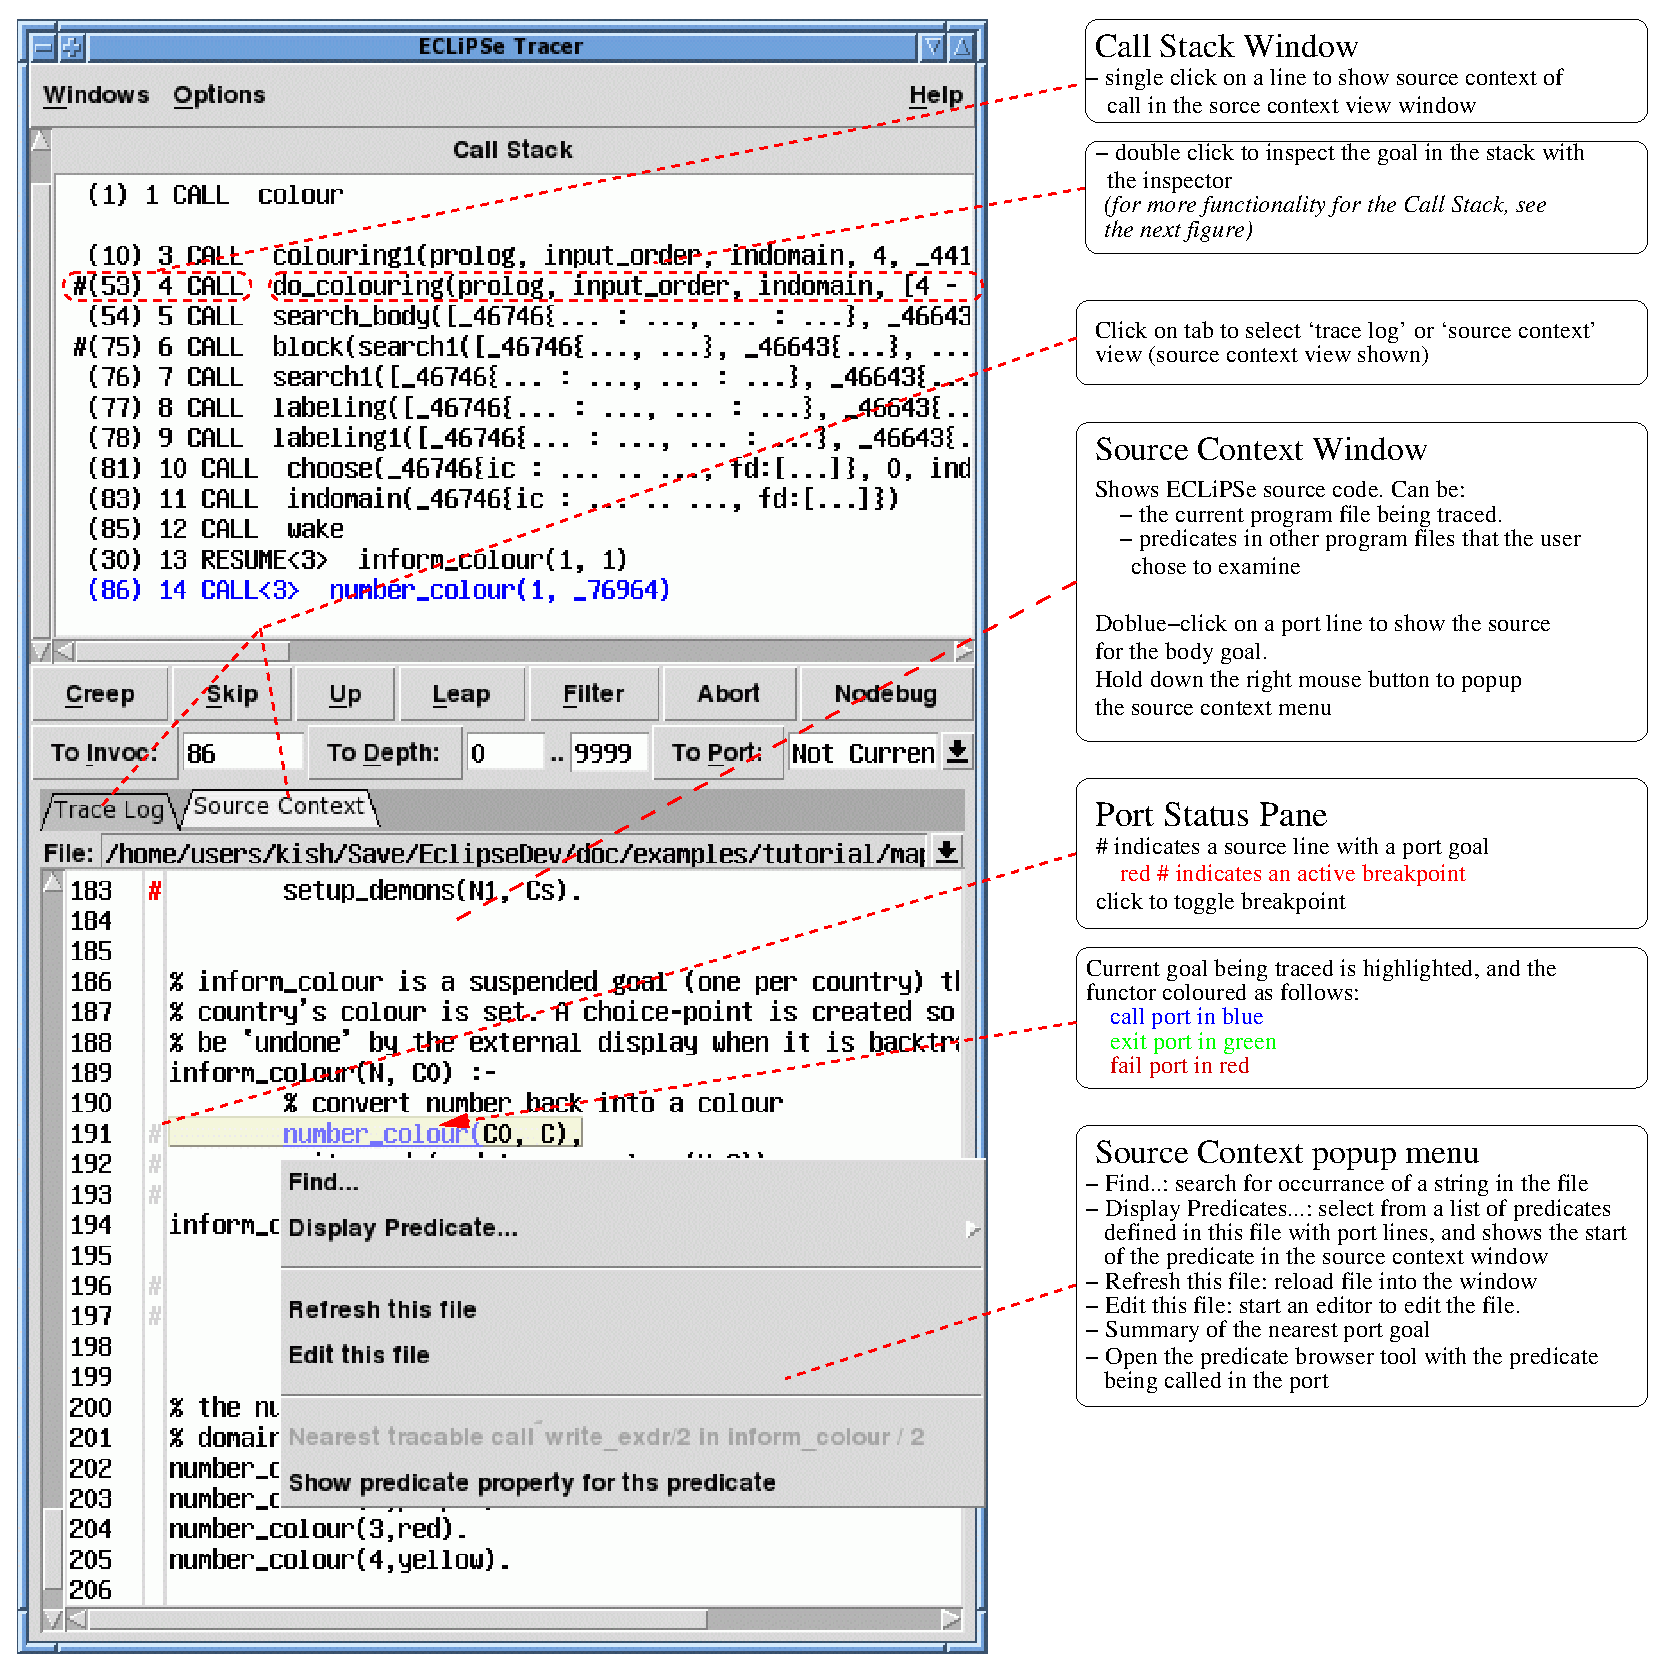
\includegraphics{tktracersourceann.eps}}

\resizebox{0.8\textwidth}{!}{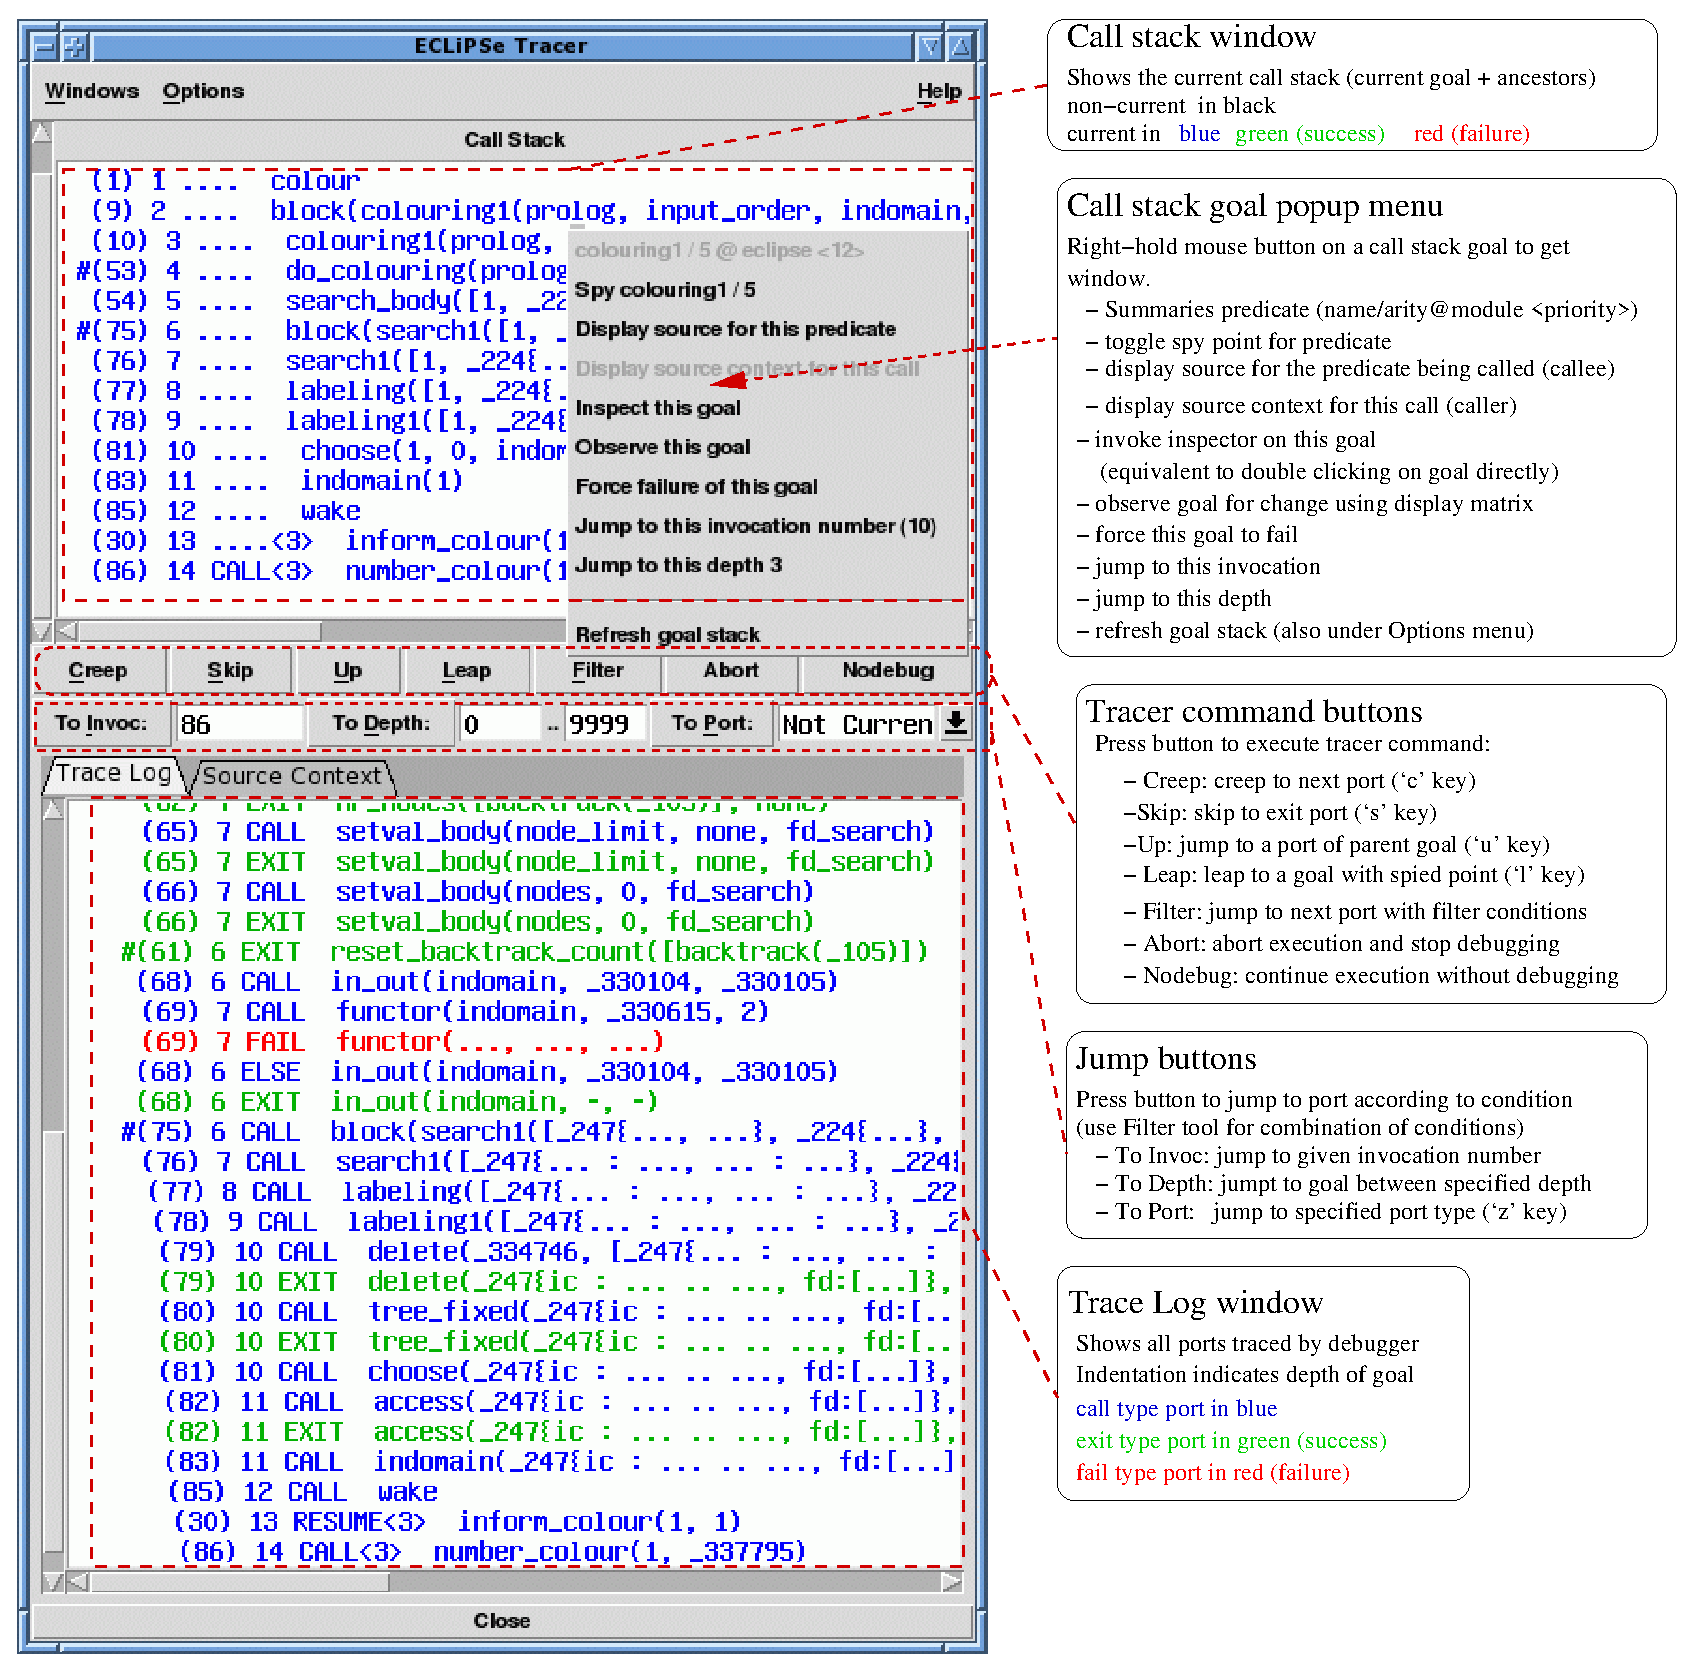
\includegraphics{tktracerann.eps}}

\menu{Options} menu options:
\begin{small}
\begin{description}
\item[Configure filter] Starts the tracer filter window, to allow the
  filter to be configured.
\item[Change print options] Changes the way the tracelines are printed.
\item[Analyse failure] Get the invocation number of the most recent failure
  so that a new run of the  query can jump to its call port.
\item[Refresh goal stack now] Refreshes the Call Stack's display.
\item[Refresh goal stack at every trace line] Select check box to allow the
  call stack to be refreshed automatically every time the tracer stops
\item[Refresh delay goals at every trace line] Select check box to allow
  the Delayed goals viewer to be automatically refreshed every time the
  tracer stops.
\item[Raise tracer window at every tracer line] Select check box to allow
  the tracer window to be raised (uncovered) automatically every time the
  tracer stops.
\end{description}
\end{small}

\subsection{Tracer Filter}
\index{tracer filter, development tool}

\resizebox{0.75\textwidth}{!}{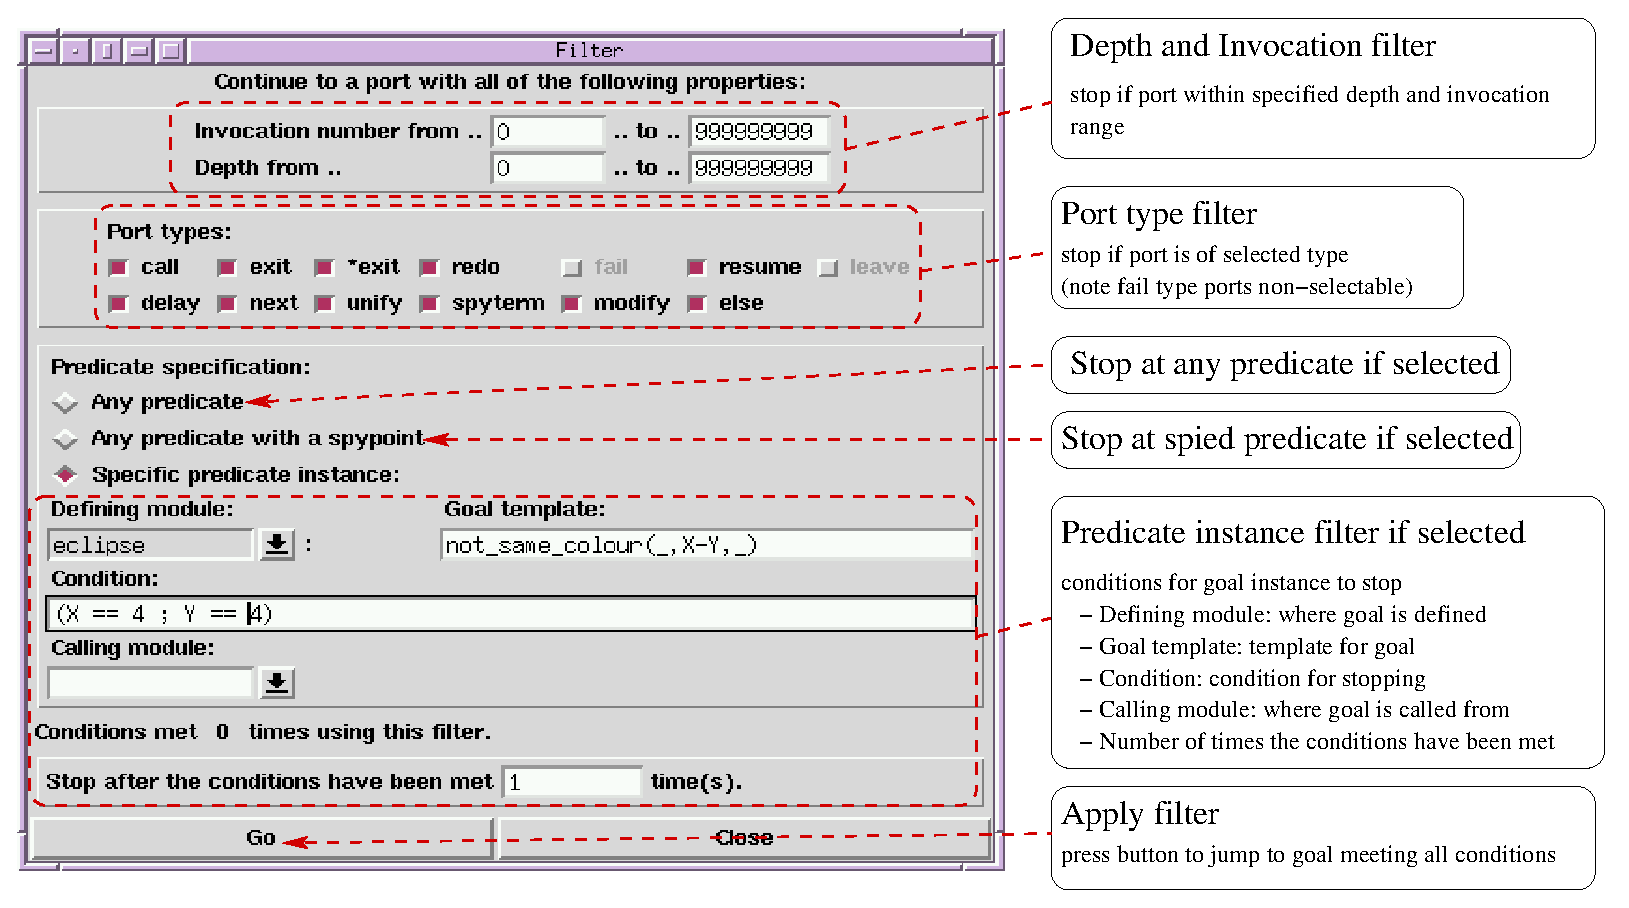
\includegraphics{tkfilterann.eps}}

\subsection{Term Inspector}
\index{term inspector, development tool}

\resizebox{0.8\textwidth}{!}{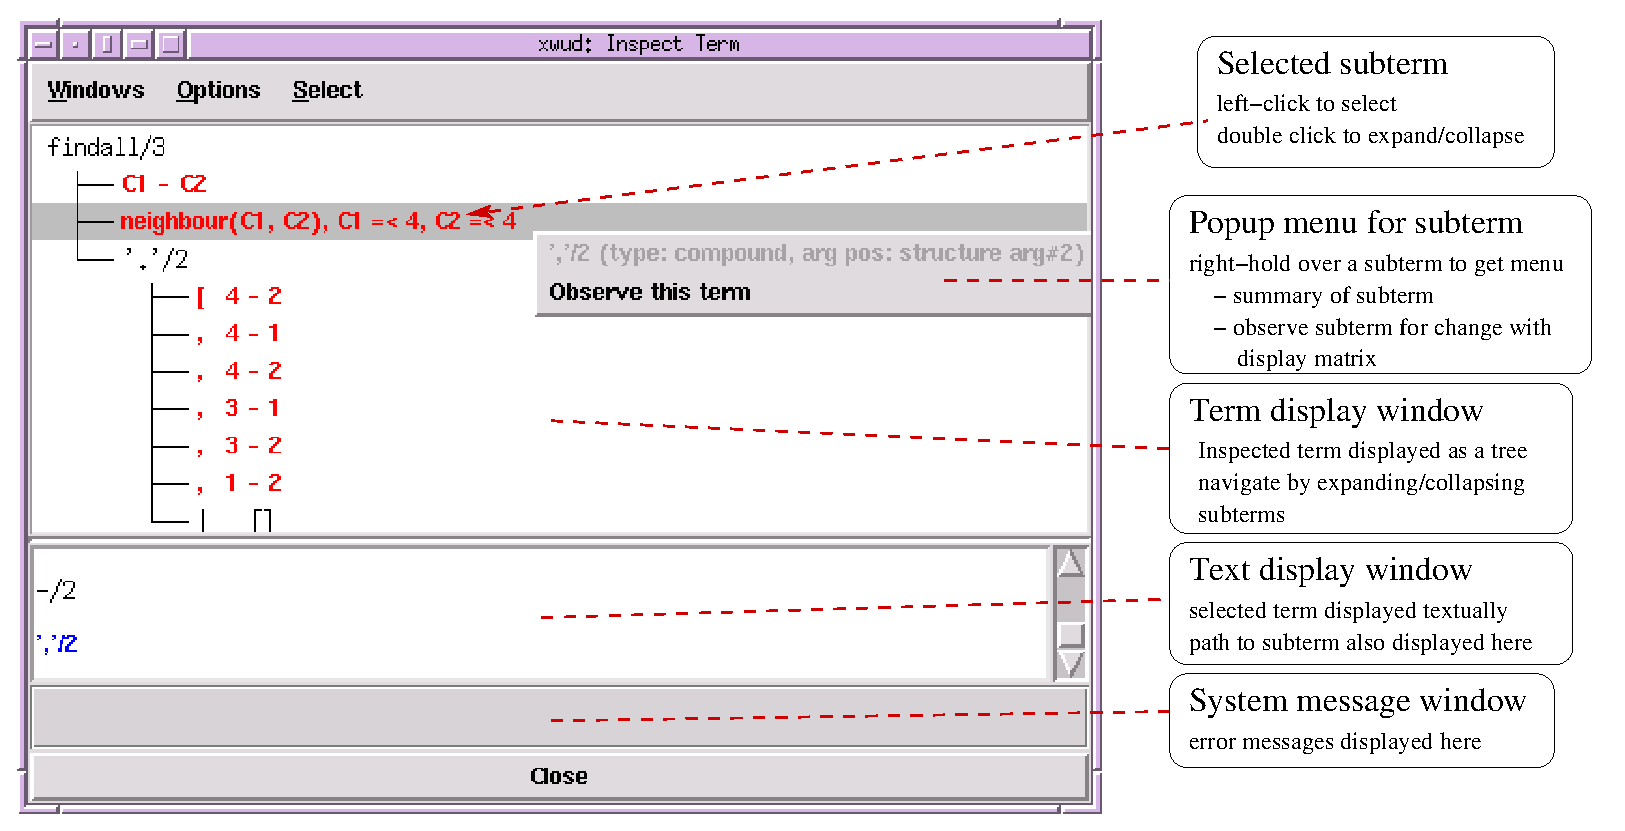
\includegraphics{tkinspectann.eps}}


%HEVEA\cutend

% BEGIN LICENSE BLOCK
% Version: CMPL 1.1
%
% The contents of this file are subject to the Cisco-style Mozilla Public
% License Version 1.1 (the "License"); you may not use this file except
% in compliance with the License.  You may obtain a copy of the License
% at www.eclipse-clp.org/license.
% 
% Software distributed under the License is distributed on an "AS IS"
% basis, WITHOUT WARRANTY OF ANY KIND, either express or implied.  See
% the License for the specific language governing rights and limitations
% under the License. 
% 
% The Original Code is  The ECLiPSe Constraint Logic Programming System. 
% The Initial Developer of the Original Code is  Cisco Systems, Inc. 
% Portions created by the Initial Developer are
% Copyright (C) 2006 Cisco Systems, Inc.  All Rights Reserved.
% 
% Contributor(s): 
% 
% END LICENSE BLOCK

%----------------------------------------------------------------------
\chapter{Program Analysis}
\label{sec:program-analysis}
\index{program analysis|(}
%HEVEA\cutdef[1]{section}
%----------------------------------------------------------------------

This chapter describes some of the tools provided by \eclipse{} to
analyse the runtime behaviour of a program.
\index{performance}\index{optimisation}
%----------------------------------------------------------------------
\section{What tools are available?}
%----------------------------------------------------------------------

\eclipse{} provides a number of different tools to help the programmer
understand their how their program behaves at runtime.

\quickrefstatic{Available Program Analysis tools}{
\begin{small}
\begin{description}
\item[Debugger] Provides a low level view of program
activity. \See{See chapter~\ref{chapdebug} and the \emph{Debugging}
section in the user manual for a comprehensive look at debugging
\eclipse{} programs}
\item[Profiler] Samples the running program at regular intervals to
give a statistical summary of where the execution time is spent.
\item[Port Profiler] Collects statistics about program execution in terms
of the box model of execution. See library(port_profiler) or use the
\emph{Port Profile} option from the tkeclipse \emph{Run} menu.
\item[Coverage] Records the number of times various parts of the
program are executed.
\item[Visualisation framework] \See{See the \emph{Visualisation Tools Manual} for more information}
\end{description}
\end{small}
}

This section focuses on two complementary tools
\begin{enumerate}
\item The \emph{profiler}
\item The \emph{coverage} library
\end{enumerate}

%----------------------------------------------------------------------
\section{Profiler}
%----------------------------------------------------------------------

\index{profiling} The profiling tool helps to find \emph{hot spots} in
a program that are worth optimising. It can be used any time with any
compiled Prolog code, it is not necessary to use a special compilation
mode or set any flags.  Note however that it is not available on
Windows\index{windows}.  When
\begin{quote}\begin{verbatim}
?- profile(Goal).
\end{verbatim}\end{quote}
\index{profile/1} is called, the profiler executes the \emph{Goal} in
the profiling mode, which means that every 100th of a second the
execution is interrupted and the profiler records the currently
executing procedure.

Consider the following \textbf{n-queens} code.
\begin{code}
queen(Data, Out) :-
        qperm(Data, Out),
        safe(Out).

qperm([], []).
qperm([X|Y], [U|V]) :-
        qdelete(U, X, Y, Z),
        qperm(Z, V).

qdelete(A, A, L, L).
qdelete(X, A, [H|T], [A|R]) :-
        qdelete(X, H, T, R).

safe([]).
safe([N|L]) :-
        nodiag(L, N, 1),
        safe(L).

nodiag([], _, _).
nodiag([N|L], B, D) :-
        D =\verb+\+= N - B,
        D =\verb+\+= B - N,
        D1 is D + 1,
        nodiag(L, B, D1).
\end{code}

Issuing the following query will result in the profiler recording the
currently executing goal 100 times a second.

\begin{quote}\begin{verbatim}
?- profile(queen([1,2,3,4,5,6,7,8,9],Out)).
goal succeeded

                PROFILING STATISTICS
                --------------------

Goal:             queen([1, 2, 3, 4, 5, 6, 7, 8, 9], Out)
Total user time:  0.03s

Predicate             Module        %Time   Time   %Cum
--------------------------------------------------------
qdelete           /4  eclipse       50.0%   0.01s  50.0%
nodiag            /3  eclipse       50.0%   0.01s 100.0%

Out = [1, 3, 6, 8, 2, 4, 9, 7, 5]
Yes (0.14s cpu)
\end{verbatim}\end{quote}

From the above result we can see how the profiler output contains four
important areas of information:
\begin{enumerate}
\item The first line of output indicates whether the specified goal
\textbf{succeeded}, \textbf{failed} or \textbf{aborted}.  The
\verb+profile/1+ predicate itself always succeeds.
\item The line beginning \verb+Goal:+ shows the goal which was
profiled.
\item The next line shows the time spent executing the goal.
\item Finally the predicates which were being executed when the
profiler sampled, ranked in decreasing sample count order are shown.
\end{enumerate}

The problem with the results displayed above is that the sampling
frequency is too low when compared to the total user time spent
executing the goal.  In fact in the above example the profiler was
only able to take two samples before the goal terminated.

The frequency at which the profiler samples is fixed, so in order to
obtain more representative results one should have an auxiliary
predicate which calls the goal a number of times, and compile and
profile a call to this auxiliary predicate. eg.

\begin{code}
queen_100 :-
  (for(_,1,100,1) do queen([1,2,3,4,5,6,7,8,9],_Out)).
\end{code}

Note that, when compiled, the above \verb+do/2+ loop would be
efficiently implemented and not cause overhead that would distort the
measurement.  \See{See section \ref{sec:loops} for more information on
logical loops}

\begin{quote}\begin{verbatim}
?- profile(queen_100).
goal succeeded

                PROFILING STATISTICS
                --------------------

Goal:             queen_100
Total user time:  3.19s

Predicate             Module        %Time   Time   %Cum
--------------------------------------------------------
nodiag            /3  eclipse       52.2%   1.67s  52.2%
qdelete           /4  eclipse       27.4%   0.87s  79.6%
qperm             /2  eclipse       17.0%   0.54s  96.5%
safe              /1  eclipse        2.8%   0.09s  99.4%
queen             /2  eclipse        0.6%   0.02s 100.0%

Yes (3.33s cpu)
\end{verbatim}\end{quote}

In the above example, the profiler takes over three hundred samples
resulting in a more accurate view of where the time is being spent in
the program.  In this instance we can see that more than half of the
time is spent in the \verb+nodiag/3+ predicate, making it an ideal
candidate for optimisation.  This is left as an exercise for the
reader.


%----------------------------------------------------------------------
\section{Line coverage}
%----------------------------------------------------------------------
\index{library!coverage}
\index{coverage}
\index{line coverage}
The line coverage library provides a means to ascertain exactly how
many times individual clauses are called during the evaluation of a
query.

\index{coverage counters}
The library works by placing \emph{coverage counters} at strategic
points throughout the code being analysed.  These counters are
incremented each time the evaluation of a query passes them.  There
are three locations in which coverage counters can be inserted.
\quickrefstatic{Locations where coverage counters can be placed}{
\begin{enumerate}
\item At the beginning of a code block.
\item Between predicate calls within a code block.
\item At the end of a code block.
\end{enumerate}
}
A code block is defined to be a conjunction of predicate calls. ie. a
sequence of goals separated by commas.

As previously mentioned, by default, code coverage counters are
inserted before and after every subgoal in the code. For instance, in
the clause
\begin{code}
p :- q, r, s.
\end{code}
four counters would be inserted: before the call to \verb+q+, between
\verb+q+ and \verb+r+, between \verb+r+ and \verb+s+, and after
\verb+s+:
\begin{quote}\begin{verbatim}
p :- point(1), q, point(2), r, point(3), s, point(4).
\end{verbatim}\end{quote}


This is the most precise form provided. The counter values do not only
show whether all code points were reached but also whether subgoals
failed or aborted (in which case the counter before a subgoal will
have a higher value than the counter after it). For example, the
result of running the above code is:
\begin{quote}\begin{alltt}
p :- \HighGreen{43 } q, \HighGreen{25 } r, \HighGreen{25 } s \HighRed{0 } .
\end{alltt}\end{quote}

which indicates that \verb+q+ was called 43 times, but succeeded only
25 times, \verb+r+ was called 25 times and succeeded always, and
\verb+s+ was called 25 times and never succeeded. Coverage counts of
zero are displayed in red (the final box) because they indicate
unreached code.  The format of the display is explained in the next
section.

%----------------------------------------------------------------------
\subsection{Compilation}
%----------------------------------------------------------------------
\index{ccompile/1}
\index{ccompile!coverage}
In order to add the coverage counters to code, it must be compiled with
the \bipref{ccompile/1}{../bips/lib/coverage/ccompile-1.html}
predicate which can be found in the
\bipref{coverage}{../bips/lib/coverage/index.html} library.

The predicate \verb+ccompile/1+ (note the initial `c' stands for
coverage) can be used in place of the normal \verb+compile/1+
predicate to compile a file with coverage counters.

Here we see the results of compiling the \textbf{n-queens} example
given in the previous section.
\begin{quote}\begin{verbatim}
?- coverage:ccompile(queens).
coverage: inserted 22 coverage counters into module eclipse
foo.ecl    compiled traceable 5744 bytes in 0.00 seconds

Yes (0.00s cpu)
\end{verbatim}\end{quote}

Once compiled, predicates can be called as usual and will (by default)
have no visible side effects.  Internally however, the counters will
be incremented as the execution progresses.  To see this in action,
consider issuing the following query having compiled the previously
defined code using \verb+ccompile/1+.
\begin{quote}\begin{alltt}
?- queens([1,2,3,4,5,6,7,8,9], Out).
\end{alltt}\end{quote}

The default behaviour of the \verb+ccompile/1+ predicate is to place
coverage counters as explained above, however such a level of detail
may be unnecessary.  If one is interested in reachability analysis the
two argument predicate \verb+ccompile/2+ \index{ccompile/2}
\index{ccompile!coverage} can take a list of \verb+name:value+ pairs
which can be used to control the exact manner in which coverage
counters are inserted.\See{See
\bipref{ccompile/2}{../bips/lib/coverage/ccompile-2.html} for a
full list of the available flags.}  In particular by specifying the
option \verb+blocks_only:on+, counters will only be inserted at the
beginning and end of code blocks. Reusing the above example this would
result in counters at point(1) and point(4).

\begin{quote}\begin{alltt}
p :- \HighGreen{43 } q,  r,  s \HighRed{0 } .
\end{alltt}\end{quote}

This can be useful in tracking down unexpected failures by looking for
exit counters which differ from entry counters, for example.


%----------------------------------------------------------------------
\subsection{Results}
%----------------------------------------------------------------------

\index{result/1} \index{result!coverage} To generate an html file
containing the coverage counter results issue the following query.
\begin{quote}\begin{verbatim}
?- coverage:result(queens).
\end{verbatim}\end{quote}
This will create the result file \texttt{coverage/queens.html} which
can be viewed using any browser.  It contains a pretty-printed form of
the source, annotated with the values of the code coverage counters as
described above. An example is shown in figure \ref{fig:queens}.

\begin{figure}
\begin{center}
\resizebox{0.5\textwidth}{!}{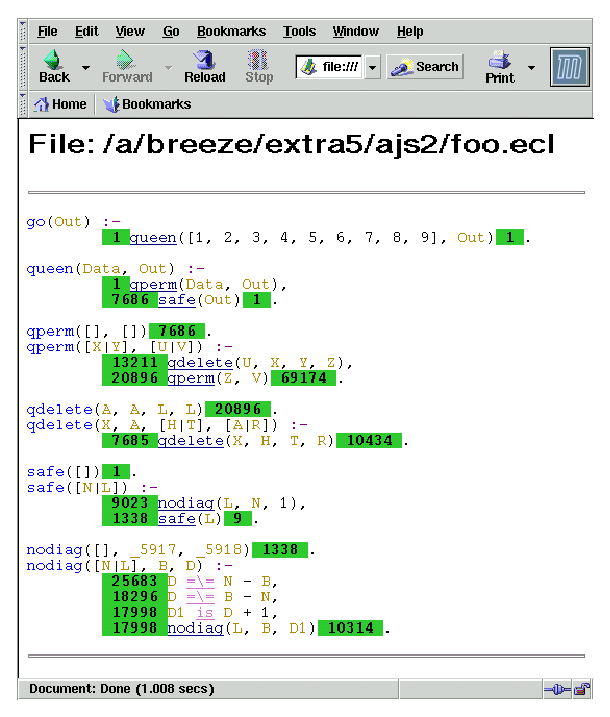
\includegraphics{coverage.eps}}
\end{center}
\caption{Results of running queens([1,2,3,4,5,6,7,8,9],_)}
\label{fig:queens}
\end{figure}

\index{result/0} \index{result!coverage} For extra convenience the
predicate \verb+result/0+ is provided which will create results for
all files which have been compiled with coverage counters.

\quickref{Result generating commands}{
\begin{description}
\item[\bipref{result/0}{../bips/lib/coverage/result-0.html}] Creates
results for all files which have been compiled with coverage counters.
\item[\bipref{result/1}{../bips/lib/coverage/result-1.html}] This
predicate takes a single argument which is the name of the file to
print the coverage counters for.
\item[\bipref{result/2}{../bips/lib/coverage/result-2.html}]
\index{result/2} The result predicate has a two argument form, the
second argument defining a number of flags which control (amongst
other things)
\begin{itemize}
\item The directory in which to create the results file. Default:
\texttt{coverage}.
\item The format of the results file (html or text). Default:
\texttt{html}.
\end{itemize}
\end{description}
\See{See \bipref{coverage}{../bips/lib/coverage/index.html} library
and \bipref{pretty_printer}{../bips/lib/pretty_printer/index.html}
library for more details}
}

\index{reset_counters/0} \index{reset_counters!coverage} Having
generated and viewed results for one run, the coverage counters can be
reset by calling
\begin{quote}\begin{verbatim}
?- coverage:reset_counters.

Yes (0.00s cpu)
\end{verbatim}\end{quote}

\index{program analysis|)}
%HEVEA\cutend

% BEGIN LICENSE BLOCK
% Version: CMPL 1.1
%
% The contents of this file are subject to the Cisco-style Mozilla Public
% License Version 1.1 (the "License"); you may not use this file except
% in compliance with the License.  You may obtain a copy of the License
% at www.eclipse-clp.org/license.
% 
% Software distributed under the License is distributed on an "AS IS"
% basis, WITHOUT WARRANTY OF ANY KIND, either express or implied.  See
% the License for the specific language governing rights and limitations
% under the License. 
% 
% The Original Code is  The ECLiPSe Constraint Logic Programming System. 
% The Initial Developer of the Original Code is  Cisco Systems, Inc. 
% Portions created by the Initial Developer are
% Copyright (C) 2006 Cisco Systems, Inc.  All Rights Reserved.
% 
% Contributor(s): 
% 
% END LICENSE BLOCK

%----------------------------------------------------------------------
\chapter{An Overview of the Constraint Libraries}
%HEVEA\cutdef[1]{section}
%----------------------------------------------------------------------

%----------------------------------------------------------------------
\section{Introduction}
%----------------------------------------------------------------------
In this section we shall briefly summarize the constraint solving
libraries of \eclipse which will be discussed in the rest of this tutorial.
%No examples are given here - each solver has its own documentation
%with examples for the interested reader.


%----------------------------------------------------------------------
\section{Implementations of Domains and Constraints}
%----------------------------------------------------------------------

\subsection{Suspended Goals: {\em suspend}}
\index{suspend}
\label{shortsecsuspend}
The constraint solvers of { \eclipse } are all implemented using suspended
goals.
The simplest implementation of any constraint is to suspend it
until all its variables are sufficiently instantiated, and then test it.

The {\em suspend} solver implements this behaviour for all
the mathematical constraints of { \eclipse },
$>=$, $>$, $=:=$, =\bsl=, $=<$ and $<$.


\subsection{Interval Solver: {\em ic}}
\index{ic}
\label{shortsecic}
The standard constraint solver offered by most constraint programming
systems is the {\em finite domain} solver, which applies constraint
propagation techniques developed in the AI community \cite{VanHentenryck}.  
{ \eclipse } supports finite domain constraints via the {\em ic}
library\footnote{and the {\em fd} library which will not be addressed in this tutorial}.
The library implements finite domains of integers, together with a basic
set of constraints.

In addition, {\em ic} also allows {\em continuous domains}
(in the form of numeric intervals), and constraints
(equations and inequations) between expressions involving
variables with continuous domains.
These expressions can contain non-linear functions such as $sin$ and built-in
constants such as $pi$.
%The user can also specify any piecewise linear unary function and {\em ic}
%will apply interval reasoning on that.
Integrality is treated as a constraint, and it is possible to mix
continuous and integral variables in the same constraint.
Specialised search techniques 
({\em splitting} \cite{VanHentenryck:95} and {\em squashing} 
\cite{lhomme96boosting}) support
the solving of problems with continuous variables.

Most constraints are also available in reified form, providing
a convenient way of combining several primitive constraints.

Note that the {\em ic} library itself implements only a standard,
basic set of arithmetic constraints. 
Many more finite domain
constraints can be defined, which have uses in specific applications.
The behaviour of these constraints is to prune the finite domains of
their variables, in just the same way as the standard constraints.
\eclipse{} offers several further libraries which implement such
constraints using the underlying domain of the {\em ic} library. 


\subsection{Global Constraints: {\em ic\_global}}
\index{ic_global}
\label{shortsecglobal}
\label{secglobalcstr}
One such library is {\em ic\_global}.
It supports a variety of constraints, each of which takes as an argument
a list of finite domain variables, of unspecified length.
Such constraints are called ``global'' constraints  \cite{beldiceanu}.
Examples of such constraints, available from the {\em ic\_global} library
are
\verb0alldifferent/10, \verb0maxlist/20, \verb0occurrences/30 and
\verb0sorted/20.
For more details see section \ref{secglobal} in chapter \ref{chapicintro}.


\subsection{Scheduling Constraints: {\em ic_cumulative, ic_edge_finder}}
\index{cumulative}
\index{edge_finder}
\label{shortsecsched}
There are several { \eclipse } libraries implementing global constraints for
scheduling applications.
The constraints take a list
of tasks (start times, durations and resource needs), and a maximum
resource level. They reduce the finite domains of the task start times
by reasoning on resource bottlenecks \cite{lepape}.  Three { \eclipse } libraries
implementing scheduling constraints are
{\em ic_cumulative}, {\em ic_edge\_finder} and {\em ic_edge\_finder3}.
They implement the same constraints declaratively, but with
different time complexity and strength of propagation.
For more details see the library documentation in the Reference Manual.



\subsection{Finite Integer Sets: {\em ic_sets}}
\index{ic_sets}
\label{shortsecsets}
The {\em ic_sets} library
implements constraints over the domain of finite
sets of integers\footnote{
the other set solvers lib(conjunto) and lib(fd_sets) are similar but not
addressed in this tutorial}.
The constraints are the usual relations over sets,
e.g.\ membership, inclusion, intersection, union, disjointness.
In addition, there are constraints between sets and integers, e.g.\
cardinality and weight constraints. For those, the {\em ic_sets} library
cooperates with the {\em ic} library.
For more details see chapter \ref{icsets}.




\subsection{Linear Constraints: {\em eplex}}
\index{eplex}
\label{shortseceplex}
{\em eplex} supports a tight integration \cite{Bockmayr} between an
external linear programming (LP) / mixed integer programming (MIP)
solver (XPRESS \cite{Dash} or CPLEX \cite{ILOG}) and { \eclipse }. 
Constraints as well as variables can be handled by the external LP/MIP
solver, by a propagation solver like {\em ic}, or by both.
Optimal solutions and other solution porperties can be returned to
\eclipse{} as required.
Search can be carried out either in \eclipse{} or in the external solver.
For more details see chapter \ref{chapeplex}.



\subsection{Constraints over symbols: {\em ic\_symbolic}}
\index{ic_symbolic}
\label{shortsecsymbolic}
The {\em ic\_symbolic} library supports variables ranging over ordered
symbolic domains (e.g. the names of products, the names of the weekdays),
and constraints over such variables. It is implemented by mapping such
variables and constraints to variables over integers and {\em ic}-constraints.


%----------------------------------------------------------------------
\section{User-Defined Constraints}
%----------------------------------------------------------------------
\subsection{Generalised Propagation: {\em propia}}
\index{propia}
\label{shortsecpropia}
The predicate {\em infers} takes as one argument
any user-defined predicate, and as a second argument a form of
propagation to be applied to that predicate.

This functionality enables the user to turn any predicate into a
constraint \cite{LeProvost93b}. The forms of propagation include finite
domains and intervals.
For more details see chapter \ref{chappropiachr}.

\subsection{Constraint Handling Rules: {\em ech}}
\index{ech}
\index{chr}
\label{shortsecech}
The user can also specify predicates using rules with guards
\cite{Fruehwirth}.  
They delay until the guard is entailed or disentailed, and then
execute or terminate accordingly. 

This functionality enables the user to implement constraints in a way
that is clearer than directly using the underlying {\em suspend}
library.
For more details see chapter \ref{chappropiachr}.


%----------------------------------------------------------------------
\section{Search and Optimisation Support}
%----------------------------------------------------------------------

\subsection{Tree Search Methods: {\em ic_search}}
\index{ic_search}
\label{shortsecsearch}
\eclipse{} has built-in backtracking and is therefore well suited for
performing depth-first tree search.
With combinatorial problems, naive depth-first search is usually not
good enough, even in the presence of constraint propagation.
It is usually necessary to apply heuristics, and if the problems are
large, one may even need to resort to incomplete search.
The {\em ic_search} contains a collection of predefined, easy-to-use
search heuristics as well as incomplete tree search strategies, applicable
to problems involving {\em ic} variables.
For more details see chapter \ref{chapsearch}.


\subsection{Optimisation: {\em branch_and_bound}}
\index{branch_and_bound}
\label{shortsecbb}
Solvers that are based on constraint propagation are typically only
concerned with satisfiability, i.e.\ with finding some or all solutions
to a problems.
The branch-and-bound method is a general technique to build optimisation
on top of a satisfiability solver.
The \eclipse{} {\em branch_and_bound} library is a solver-independent
implementation of the branch-and-bound method, and provides a number
of options and variants of the basic technique.


%----------------------------------------------------------------------
\section{Hybridisation Support}
%----------------------------------------------------------------------
\subsection{Repair and Local Search: {\em repair}}
\index{repair}
\label{shortsecrepair}
The {\em repair} library allows a {\em tentative} value to be
associated with any variable \cite{cp99wkshoptalk}.
This tentative value may violate constraints on the variable, in which
case the constraint is recorded in a list of violated constraints.
The repair library also supports propagation {\em invariants}
\cite{Localizer}.
Using invariants,  if a variable's tentative
value is changed, the consequences of this change can be propagated to
any variables whose tentative values depend on the changed one.
The use of tentative values in search is illustrated in chapter \ref{chaprepair}.
 

\subsection{Hybrid: {\em ic\_probing\_for\_scheduling}}
\index{probing_for_scheduling}
\label{shortsecprobing}
For scheduling applications where the cost is dependent on each start
time, a combination of solvers can be very powerful.
For example, we can use finite domain
propagation to reason on 
resources and linear constraint solving to reason on cost \cite{HaniProbe}.
The {\em probing\_for\_scheduling} library supports such a combination,
via a similar user interface to the {\em cumulative} constraint mentioned
above in section \ref{secglobalcstr}.
For more details see chapter \ref{chaphybrid}.


%----------------------------------------------------------------------
\section{Other Libraries}
%----------------------------------------------------------------------
The solvers described above are just a few of the many libraries
available in ECLiPSe and listed in the \eclipse{} library directory.
Any \eclipse{} user who has implemented a constraint solver is
encouraged to make it available to the user community and publicise
it via the {\tt eclipse-users@icparc.ic.ac.uk} mailing list!
Comments and suggestions on the existing libraries are also welcome!


%\bibliographystyle{alpha}
%\bibliography{solver_intro}

%\end{document}

%HEVEA\cutend

% BEGIN LICENSE BLOCK
% Version: CMPL 1.1
%
% The contents of this file are subject to the Cisco-style Mozilla Public
% License Version 1.1 (the "License"); you may not use this file except
% in compliance with the License.  You may obtain a copy of the License
% at www.eclipse-clp.org/license.
% 
% Software distributed under the License is distributed on an "AS IS"
% basis, WITHOUT WARRANTY OF ANY KIND, either express or implied.  See
% the License for the specific language governing rights and limitations
% under the License. 
% 
% The Original Code is  The ECLiPSe Constraint Logic Programming System. 
% The Initial Developer of the Original Code is  Cisco Systems, Inc. 
% Portions created by the Initial Developer are
% Copyright (C) 2006 Cisco Systems, Inc.  All Rights Reserved.
% 
% Contributor(s): 
% 
% END LICENSE BLOCK

\chapter{Getting started with Interval Constraints}
\label{chapicintro}
%HEVEA\cutdef[1]{section}

The Interval Constraints (IC) library provides a constraint solver which
works with both integer and real interval variables.
This chapter provides a general introduction to the library, and then
focusses on its support for integer constraints.
For more detail on IC's real variables and constraints, please see
Chapter~\ref{chapreal}.

%----------------------------------------------------------------------
\section{Using the Interval Constraints Library}

To use the Interval Constraints Library, load the library using either of:
\begin{code}
:- lib(ic).
:- use_module(library(ic)).
\end{code}
Specify this at the beginning of your program.

%----------------------------------------------------------------------
\section{Structure of a Constraint Program}
The typical top-level structure of a constraint program is
\begin{code}
solve(Variables) :-
        read_data(Data),
        setup_constraints(Data, Variables),
        labeling(Variables).
\end{code}
where \verb0setup_constraints/20 contains the problem model. It creates the
variables and the constraints over the variables.
This is often, but not necessarily, deterministic.
The \verb0labeling/10 predicate is the search part of the program that
attempts to find solutions by trying all instantiations for the
variables. This search is constantly pruned by constraint propagation.

The above program will find all solutions.
If the best solution is wanted, a branch-and-bound
procedure can be wrapped around the search component of the program:
\begin{code}
solve(Variables) :-
        read_data(Data),
        setup_constraints(Data, Variables, Objective),
        branch_and_bound:minimize(labeling(Variables), Objective).
\end{code}

\See{The {\em branch\_and\_bound} library provides generic predicates 
that support optimization in conjunction with any \eclipse{} solver. 
Section~\ref{secbboptsearch} discusses these predicates.}


%----------------------------------------------------------------------
\section{Modelling}
The problem modelling code must:
    \begin{itemize}
    \item Create the variables with their initial domains
    \item Setup the constraints between the variables
    \end{itemize}

A simple example is the ``crypt-arithmetic'' puzzle, 
\verb0SEND+MORE = MONEY0.
The idea is to associate a digit (0-9) with each letter so that the
equation is true. The \eclipse{} code is as follows:

\label{send-more-money}
\begin{code}
:- lib(ic).

sendmore(Digits) :-
    Digits = [S,E,N,D,M,O,R,Y],

% Assign a finite domain with each letter - S, E, N, D, M, O, R, Y - 
% in the list Digits
    Digits :: [0..9],

% Constraints
    alldifferent(Digits),
    S #\verb0\0= 0,
    M #\verb0\0= 0,
                 1000*S + 100*E + 10*N + D
               + 1000*M + 100*O + 10*R + E
    #= 10000*M + 1000*O + 100*N + 10*E + Y,

% Search
    labeling(Digits).
\end{code}

%----------------------------------------------------------------------
\section{Built-in Constraints}
\label{icbics}

The following section summarises the built-in constraint predicates of the
{\em ic} library.

\quickref{Domain constraints}{
\begin{description}

\item [\biptxtrefni{Vars :: Domain}{::/2!ic}{../bips/lib/ic/NN-2.html}]
\index{::/2@\texttt{::/2}!ic} 
Constrains Vars to take only integer or real values from the domain
specified by Domain.  Vars may be a variable, a list, or a submatrix (e.g.\
M[1..4, 3..6]); for a list or a submatrix, the domain is applied recursively
so that one can apply a domain to, for instance, a list of lists of
variables.  Domain can be specified as a simple range Lo .. Hi, or as a list
of subranges and/or individual elements (integer variables only).  The type
of the bounds determines the type of the variable (real or integer).  Also
allowed are the (untyped) symbolic bound values {\tt inf}, {\tt +inf} and
{\tt -inf}.

\item [\biptxtrefni{Vars \$:: Domain}{\$::/2!ic}{../bips/lib/ic/SNN-2.html}] 
\index{\$::/2@\texttt{\$::/2}!ic} 
Like \texttt{::/2}, but for declaring real variables (i.e.\ it never imposes
integrality, regardless of the types of the bounds).

\item [\biptxtrefni{Vars \#:: Domain}{\#::/2!ic}{../bips/lib/ic/HNN-2.html}] 
\index{\#::/2@\texttt{\#::/2}!ic} 
Like \texttt{::/2}, but for declaring integer variables.

\item [\biptxtrefni{reals(Vars)}{reals/1!ic}{../bips/lib/ic/reals-1.html}]
\index{reals/1@\texttt{reals/1}!ic} 
Declares that the variables are IC variables (like declaring
{\tt Vars :: -inf..inf}).

\item [\biptxtrefni{integers(Vars)}{integers/1!ic}{../bips/lib/ic/integers-1.html}] 
\index{integers/1@\texttt{integers/1}!ic} 
Constrains the given variables to take integer values only.

\end{description}}

The most common way to declare an IC variable is to use the
\biptxtrefni{::/2}{::/2!ic}{../bips/lib/ic/NN-2.html} predicate (or
\biptxtrefni{\$::/2}{\$::/2!ic}{../bips/lib/ic/SNN-2.html} or
\biptxtrefni{\#::/2}{\#::/2!ic}{../bips/lib/ic/HNN-2.html}) to give it an
initial domain:

\begin{quote}\begin{verbatim}
?- X :: -10 .. 10.
X = X{-10 .. 10}
Yes

?- X :: -10.0 .. 10.0.
X = X{-10.0 .. 10.0}
Yes

?- X #:: -10 .. 10.
X = X{-10 .. 10}
Yes

?- X $:: -10 .. 10.
X = X{-10.0 .. 10.0}
Yes

?- X :: 0 .. 1.0Inf.
X = X{0 .. 1.0Inf}
Yes

?- X :: 0.0 .. 1.0Inf.
X = X{0.0 .. 1.0Inf}
Yes

?- X :: [1, 4 .. 6, 9, 10].
X = X{[1, 4 .. 6, 9, 10]}
Yes
\end{verbatim}\end{quote}

Note that for \biptxtrefni{::/2}{::/2!ic}{../bips/lib/ic/NN-2.html}
\index{\#::/2@\texttt{\#::/2}!ic}  the type
of the bounds defines the type of the variable (integer or real) but that
infinities are considered type-neutral.  To just declare the type of a
variable without restricting the domain at all, one can use the
\biptxtrefni{integers/1}{integers/1!ic}{../bips/lib/ic/integers-1.html}
\index{\#::/2@\texttt{\#::/2}!ic} 
and \biptxtrefni{reals/1}{reals/1!ic}{../bips/lib/ic/reals-1.html}\index{\#::/2@\texttt{\#::/2}!ic} 
.

The final way to declare that a variable is an IC variable is to just use it
in an IC constraint: this performs an implicit declaration.

\ignore{
\begin{code}
?- X :: -10 .. 10, get_domain_as_list(X, List).
   X = X\{-10 .. 10\}
   List = [-10, -9, -8, -7, -6, -5, -4, -3, -2, -1, 0, 1, 2, 3, 4, 5, 6, 7, 8, 9, 10]
Yes

?- reals([X, Y]), X = Y, X$>= 1.5, X $=< 2.5, Y = 2.2.
   X = 2.2
   Y = 2.2
Yes

?- integers([X, Y]), X :: 0 .. 4, X + Y #= W, X = Y, W = 8.
   X = 4
   Y = 4
   W = 8
Yes
\end{code}
}

\quickref{Integral Arithmetic constraints\label{integer-constraints}}{
\begin{description}

\item [\biptxtrefni{ExprX \#= ExprY}{\#=/2!ic}{../bips/lib/ic/HE-2.html}]
\index{\#=/2@\texttt{\#=/2}!ic} 
ExprX is equal to ExprY.  ExprX and ExprY are integer expressions, and the
variables and subexpressions are constrained to be integers.

\item [\biptxtrefni{ExprX \#>= ExprY}{\#>=/2!ic}{../bips/lib/ic/HGE-2.html}]
\index{\#>=/2@\texttt{\#>=/2}!ic} 
ExprX is greater than or equal to ExprY.  ExprX and ExprY are integer
expressions, and the variables and subexpressions are constrained to be
integers.

\item [\biptxtrefni{ExprX \#=< ExprY}{\#=</2!ic}{../bips/lib/ic/HEL-2.html}]
\index{\#=</2@\texttt{\#=</2}!ic} 
ExprX is less than or equal to ExprY.  ExprX and ExprY are integer
expressions, and the variables and subexpressions are constrained to be
integers.

\item [\biptxtrefni{ExprX \#> ExprY}{\#>/2!ic}{../bips/lib/ic/HG-2.html}]
\index{\#>/2@\texttt{\#>/2}!ic} 
ExprX is greater than ExprY.  ExprX and ExprY are integer expressions, and
the variables and subexpressions are constrained to be integers.

\item [\biptxtrefni{ExprX \#< ExprY}{\#</2!ic}{../bips/lib/ic/HL-2.html}]
\index{\#</2@\texttt{\#</2}!ic} 
ExprX is less than ExprY.  ExprX and ExprY are integer expressions, and the
variables and subexpressions are constrained to be integers.

%\item [\biptxtrefni{ExprX \#\bsl= ExprY}{\#\bsl=/2!ic}{../bips/lib/ic/HRE-2.html}]
\item [{\bf ExprX \#\bsl= ExprY}]
ExprX is not equal to ExprY.  ExprX and ExprY are integer
expressions, and the variables are constrained to be integers.

\item [\biptxtref{ac_eq(X, Y, C)}{ac_eq/3}{../bips/lib/ic/ac_eq-3.html}]
Arc-consistent implementation of \bipnoidx{X \#= Y + C}.  X and Y are
constrained to be integer variables and to have ``reasonable'' bounds.  C
must be an integer.

\end{description}}
% This belongs inside the quickref, but the \bsl gets garbled in the index
% if it's there.
\index{\#\=@\#\bsl=/2!ic}%

\quickref{Non-Integral Arithmetic Constraints\label{general-constraints}}{
\begin{description}

\item [\biptxtrefni{ExprX \$= ExprY}{\$=/2!ic}{../bips/lib/ic/SE-2.html}]
\index{\$=/2@\texttt{\$=/2}!ic} ExprX is equal to ExprY.  ExprX and ExprY are general expressions.

\item [\biptxtrefni{ExprX \$>= ExprY}{\$>=/2!ic}{../bips/lib/ic/SGE-2.html}]
\index{\$>=/2@\texttt{\$>=/2}!ic} ExprX is greater than or equal to ExprY.  ExprX and ExprY are general
expressions.

\item [\biptxtrefni{ExprX \$=< ExprY}{\$=</2!ic}{../bips/lib/ic/SEL-2.html}]
\index{\$=</2@\texttt{\$=</2}!ic} ExprX is less than or equal to ExprY.  ExprX and ExprY are general expressions.

\item [\biptxtrefni{ExprX \$> ExprY}{\$>/2!ic}{../bips/lib/ic/SG-2.html}]
\index{\$>/2@\texttt{\$>/2}!ic} ExprX is greater than ExprY.  ExprX and ExprY are general expressions.

\item [\biptxtrefni{ExprX \$< ExprY}{\$</2!ic}{../bips/lib/ic/SL-2.html}]
\index{\$</2@\texttt{\$</2}!ic} ExprX is less than ExprY.  ExprX and ExprY are general expressions.

\item [{\bf ExprX \$\bsl= ExprY}]
ExprX is not equal to ExprY.  ExprX and ExprY are general expressions.
\end{description}}
% This belongs inside the quickref, but the \bsl gets garbled in the index
% if it's there.
\index{\$\=@\$\bsl=/2!ic}%

The basic IC relational constraints come in two forms.  The first form is
for integer-only constraints, and is summarised in
Figure~\ref{integer-constraints}.  All of these constraints contain
\texttt{\#} in their name, which indicates that all numbers appearing in
them must be integers, and all variables \emph{and subexpressions} will be
constrained to be integral.  It is important to note that subexpressions are
constrained to be integral, because it means, for instance, that
\bipnoidx{X/2 + Y/2 \#= 1} and \bipnoidx{X + Y \#= 2} are different
constraints, since the former constrains X and Y to be even.

The second form is the general form of the constraints, and is summarised in
Figure~\ref{general-constraints}.  These constraints can be used with either
integer or real variables and numbers.  With the exception of integrality
issues, the two versions of each constraint are equivalent.  Thus if the
constants are integers and the variables and subexpressions are integral,
the two forms may be used interchangeably.

Most of the basic constraints operate by propagating bound information
(performing interval reasoning).  The exceptions are the disequality (not
equals) constraints and the \bipnoidx{ac_eq/3} constraint, which perform
domain reasoning (arc consistency).  An example:

\begin{quote}\begin{verbatim}
?- [X, Y] :: 0 .. 10, X #>= Y + 2.
X = X{2 .. 10}
Y = Y{0 .. 8}
There is 1 delayed goal.
Yes
\end{verbatim}\end{quote}

In the above example, since the lower bound of \texttt{Y} is 0 and
\texttt{X} must be at least 2 greater, the lower bound of \texttt{X} has
been updated to 2.  Similarly, the upper bound of \texttt{Y} has been
reduced to 8.  The delayed goal indicates that the constraint is still
active: there are still some combinations of values for \texttt{X} and
\texttt{Y} which violate the constraint, so the constraint remains until it
is sure that no such violation is possible.

Note that if a domain ever becomes empty as the result of propagation (no
value for the variable is feasible) then the constraint must necessarily
have been violated, and the computation backtracks.

For a disequality constraint, no deductions can be made until
there is only one variable left, at which point (if it is an integer
variable) the variable's domain can be updated to exclude the relevant
value:

\begin{quote}\begin{verbatim}
?- X :: 0 .. 10, X #\= 3.
X = X{[0 .. 2, 4 .. 10]}
Yes

?- [X, Y] :: 0 .. 10, X - Y #\= 3.
X = X{0 .. 10}
Y = Y{0 .. 10}
There is 1 delayed goal.
Yes

?- [X, Y] :: 0 .. 10, X - Y #\= 3, Y = 2.
X = X{[0 .. 4, 6 .. 10]}
Y = 2
Yes
\end{verbatim}\end{quote}

For the \bipref{ac_eq/3}{../bips/lib/ic/ac_eq-3.html} constraint, ``holes''
in the domain of one variable are propagated to the other:

\begin{quote}\begin{verbatim}
?- [X, Y] :: 0 .. 10, ac_eq(X, Y, 3).
X = X{3 .. 10}
Y = Y{0 .. 7}
There is 1 delayed goal.
Yes

?- [X, Y] :: 0 .. 10, ac_eq(X, Y, 3), Y #\= 4.
X = X{[3 .. 6, 8 .. 10]}
Y = Y{[0 .. 3, 5 .. 7]}
There is 1 delayed goal.
Yes
\end{verbatim}\end{quote}

Compare with the corresponding bounds consistency constraint:

\begin{quote}\begin{verbatim}
?- [X, Y] :: 0 .. 10, X #= Y + 3, Y #\= 4.
X = X{3 .. 10}
Y = Y{[0 .. 3, 5 .. 7]}
There is 1 delayed goal.
Yes
\end{verbatim}\end{quote}

\See{IC supports a range of mathematical operators beyond the basic
\texttt{+/2}, \texttt{-/2}, \texttt{*/2}, etc.  See the IC chapter in
the Constraint Library Manual for full details.}

\Note{If one wishes to construct an expression to use in an IC constraint at
run time, then one must wrap it in \texttt{eval/1}:}

\begin{quote}\begin{verbatim}
?- [X, Y] :: 0..10, Expr = X + Y, Sum #= Expr.
number expected in set_up_ic_con(7, 1, [0 * 1, 1 * Sum{-1.0Inf .. 1.0Inf}, -1 * (X{0 .. 10} + Y{0 .. 10})])
Abort

?- [X, Y] :: 0..10, Expr = X + Y, Sum #= eval(Expr).
X = X{0 .. 10}
Y = Y{0 .. 10}
Sum = Sum{0 .. 20}
Expr = X{0 .. 10} + Y{0 .. 10}
There is 1 delayed goal.
Yes
\end{verbatim}\end{quote}

{\em Reification} provides access to the logical truth of a constraint
expression and can be used by:

\begin{itemize}
\item The {\eclipse} system to infer the truth value, reflecting the value 
into a variable.
\item The programmer to enforce the constraint or its negation by giving a
value to the truth variable.
\end{itemize}

This logical truth value is a boolean variable (domain \texttt{0..1}), where
the value 1 means the constraint is or is required to be true, and the value
0 means the constraint is or is required to be false.

When constraints appear in an expression context, 
they evaluate to their reified truth value. Practically, this means that 
the constraints are posted in a passive check but do not propagate mode.
In this mode no variable domains are modified but checks are made to
determine whether the constraint has become entailed (necessarily true) or 
disentailed (necessarily false).

The simplest and arguably most natural way to reify a constraint is to
place it in an expression context  (i.e.\ on either side of a \verb|$=|,
\verb|#=|, etc.) and assign its truth value to a variable. For example:

\begin{quote}\begin{verbatim}
?- X :: 0 .. 10, TruthValue $= (X $> 4).
TruthValue = TruthValue{[0, 1]}
X = X{0 .. 10}
There is 1 delayed goal.
Yes

?- X :: 6 .. 10, TruthValue $= (X $> 4).
TruthValue = 1
X = X{6 .. 10}
Yes

?- X :: 0 .. 4, TruthValue $= (X $> 4).
TruthValue = 0
X = X{0 .. 4}
Yes
\end{verbatim}\end{quote}

All the basic relational constraint predicates also come in a three-argument
form where the third argument is the reified truth value, and this form can
also be used to reify a constraint directly.  For example:

\begin{quote}\begin{verbatim}
?- X :: 0 .. 10, $>(X, 4, TruthValue).
X = X{0 .. 10}
TruthValue = TruthValue{[0, 1]}
There is 1 delayed goal.
Yes
\end{verbatim}\end{quote}

As noted above the boolean truth variable corresponding to a constraint can
also be used to enforce the constraint (or its negation):

\begin{quote}\begin{verbatim}
?- X :: 0 .. 10, TruthValue $= (X $> 4), TruthValue = 1.
X = X{5 .. 10}
TruthValue = 1
Yes

?- X :: 0 .. 10, TruthValue $= (X $> 4), TruthValue = 0.
X = X{0 .. 4}
TruthValue = 0
Yes
\end{verbatim}\end{quote}

By instantiating the value of the reified truth variable, the constraint
changes from being {\em passive} to being {\em active}.  Once actively
true (or actively false) the constraint will prune domains as though
it had been posted as a simple non-reified constraint.

\ignore{
\Note{User defined constraints will be treated as reifiable if they appear
in an expression context and as such should provide a version with an extra
argument where this final argument is the reified truth value reflected
into a variable.}
}

\See{Additional information on reified constraints can be found in the
{\eclipse} Constraint Library Manual that documents {\em IC: A Hybrid
 Finite Domain / Real Number Interval Constraint Solver}.}


\quickref{Constraint Expression Connectives\label{expression-connectives}}{
\begin{description}

\item[{\bf and}]
     Constraint conjunction. e.g.\ {\tt X \$> 3 and X \$< 8}

\item[{\bf or}]
     Constraint disjunction. e.g.\ {\tt X \$< 3 or X \$> 8}

\item[{\bf =>}]
     Constraint implication. e.g.\ {\tt X \$> 3 => Y \$< 8}

\item[{\bf neg}]
     Constraint negation. e.g.\ {\tt neg X \$> 3}

\end{description}}

IC also provides a number of connectives useful for combining constraint
expressions.  These are summarised in Figure~\ref{expression-connectives}.
For example:

\begin{quote}\begin{verbatim}
?- [X, Y] :: 0 .. 10, X #>= Y + 6 or X #=< Y - 6.
X = X{0 .. 10}
Y = Y{0 .. 10}
There are 3 delayed goals.
Yes

?- [X, Y] :: 0 .. 10, X #>= Y + 6 or X #=< Y - 6, X #>= 5.
Y = Y{0 .. 4}
X = X{6 .. 10}
There is 1 delayed goal.
Yes
\end{verbatim}\end{quote}

In the above example, once it is known that \texttt{X \#=< Y - 6} cannot be
true, the constraint \texttt{X \#>= Y + 6} is enforced.

Note that these connectives exploit constraint reification, and actually
just reason about boolean variables.  This means that they can be used as
boolean constraints as well:

\begin{quote}\begin{verbatim}
?- A => B.
A = A{[0, 1]}
B = B{[0, 1]}
There is 1 delayed goal.
Yes

?- A => B, A = 1.
B = 1
A = 1
Yes

?- A => B, A = 0.
B = B{[0, 1]}
A = 0
Yes
\end{verbatim}\end{quote}


%----------------------------------------------------------------------

\section{Global constraints}
\label{secglobal}

\index{global constraints!ic|(}
\index{library!ic_global|(}

The IC constraint solver has some optional components which provide
so-called \emph{global} constraints.  These are high-level constraints that
tend to provide more global reasoning than the constraints in the main IC
library.  These optional components are contained in the \texttt{ic_global},
\texttt{ic_cumulative},\index{library!ic_cumulative}
\texttt{ic_edge_finder}\index{library!ic_edge_finder}
and \texttt{ic_edge_finder3}\index{library!ic_edge_finder3}
libraries.  The \texttt{ic_global} library provides a collection of general
global constraints, while the others provide constraints for
resource-constrained scheduling.

To use these global constraints, load the relevant optional library or
libraries using directives in one of these forms:
\begin{code}
:- lib(ic_global).
:- use_module(library(ic_global)).
\end{code}
Specify this at the beginning of your program.

Note that some of these libraries provide alternate implementations of
predicates which also appear in other libraries.  For example, the
\texttt{alldifferent/1} constraint is provided by both the standard
\texttt{ic} library and the \texttt{ic_global} library.  This means that if
you wish to use it, you must use the relevant module qualifier to specify
which one you want:
\biptxtrefni{ic:alldifferent/1}{alldifferent/1!ic}{../bips/lib/ic/alldifferent-1.html} 
\index{alldifferent/1@\texttt{alldifferent/1}!ic} or \index{alldifferent/1@\texttt{alldifferent/1}!ic_global}
\biptxtrefni{ic_global:alldifferent/1}{alldifferent/1!ic_global}{../bips/lib/ic_global/alldifferent-1.html}.

% List a few example predicates from ic_global?

\See{See the ``Additional Finite Domain Constraints'' section of the Library
Manual for more details of these libraries and a full list of the predicates
they provide.}


\subsection{Different strengths of propagation}

The \texttt{alldifferent(List)} predicate imposes the constraint on the
elements of \texttt{List} that they all take different values.
The standard \biptxtrefni{alldifferent/1}{alldifferent/1!ic}{../bips/lib/ic/alldifferent-1.html}
\index{alldifferent/1@\texttt{alldifferent/1}!ic} predicate from the IC library provides a level of propagation equivalent to
imposing pairwise
%\biptxtrefni{\#\bsl=/2}{\#\=/2@\#\bsl=/2!ic}{../bips/lib/ic/HRE-2.html}
\ahref{../bips/lib/ic/HRE-2.html}{{\bf \#\bsl=/2}}
\index{\#\=@\#\bsl=/2!ic}%
constraints (though it does it more efficiently than that).  This means that
no propagation is performed until elements of the list start being made
ground.  This is despite the fact that there may be ``obvious'' inferences
which could be made.

Consider as an example the case of 5 variables with domains \texttt{1..4}.
Clearly the 5 variables cannot all be given different values, since there
are only 4 distinct values available.  However, the standard
\biptxtrefni{alldifferent/1}{alldifferent/1!ic}{../bips/lib/ic/alldifferent-1.html} constraint
cannot determine this:

\begin{quote}\begin{verbatim}
?- L = [X1, X2, X3, X4, X5], L :: 1 .. 4, ic:alldifferent(L).
X1 = X1{1 .. 4}
X2 = X2{1 .. 4}
X3 = X3{1 .. 4}
X4 = X4{1 .. 4}
X5 = X5{1 .. 4}
L = [X1{1 .. 4}, X2{1 .. 4}, X3{1 .. 4}, X4{1 .. 4}, X5{1 .. 4}]
There are 5 delayed goals.
Yes
\end{verbatim}\end{quote}

Consider another example where three of the variables have domain
\texttt{1..3}.  Clearly, if all the variables are to be different, then no
other variable can take a value in the range \texttt{1..3}, since each of
those values must be assigned to one of the original three variables.
Again, the standard 
\biptxtrefni{alldifferent/1}{alldifferent/1!ic}{../bips/lib/ic/alldifferent-1.html} constraint 
cannot determine this:

\begin{quote}\begin{verbatim}
?- [X1, X2, X3] :: 1 .. 3, [X4, X5] :: 1 .. 5,
   ic:alldifferent([X1, X2, X3, X4, X5]).
X1 = X1{1 .. 3}
X2 = X2{1 .. 3}
X3 = X3{1 .. 3}
X4 = X4{1 .. 5}
X5 = X5{1 .. 5}
There are 5 delayed goals.
Yes
\end{verbatim}\end{quote}

On the other hand, \texttt{ic_global}'s
\biptxtrefni{alldifferent/1}{alldifferent/1!ic_global}{../bips/lib/ic_global/alldifferent-1.html}
\index{alldifferent/1@\texttt{alldifferent/1}!ic_global}
constraint performs some stronger, more global reasoning, and for both of
the above examples makes the appropriate inference:

\begin{quote}\begin{verbatim}
?- L = [X1, X2, X3, X4, X5], L :: 1 .. 4, ic_global:alldifferent(L).
No

?- [X1, X2, X3] :: 1 .. 3, [X4, X5] :: 1 .. 5,
   ic_global:alldifferent([X1, X2, X3, X4, X5]).
X1 = X1{1 .. 3}
X2 = X2{1 .. 3}
X3 = X3{1 .. 3}
X4 = X4{[4, 5]}
X5 = X5{[4, 5]}
There are 2 delayed goals.
Yes
\end{verbatim}\end{quote}

Of course, there is a trade-off here: the stronger version of the constraint
takes longer to perform its propagation.  Which version is best depends on
the nature of the problem being solved.

\See{Note that even stronger propagation can be achieved if desired, by
using the Propia library (see Chapter~\ref{chappropiachr}).}

\index{library!ic_global|)}

In a similar vein, the \texttt{ic_cumulative}, \texttt{ic_edge_finder} and
\texttt{ic_edge_finder3} libraries provide increasingly strong versions of
constraints such as \texttt{cumulative/4}, but with increasing cost to do
their propagation (linear, quadratic and cubic, respectively).

\index{global constraints!ic|)}

%----------------------------------------------------------------------

\section{Simple User-defined Constraints}
User-defined, or `conceptual' constraints can easily be defined as 
conjunctions of primitive constraints. For example, let us consider a set 
of products and the specification that allows them to be colocated in a 
warehouse. This should be done in such a way as to propagate possible 
changes in the domains as soon as this becomes possible.  

Let us assume we have a symmetric relation that defines which product
can be colocated with another and that products are distinguished by numeric 
product identifiers: 

\begin{code}
colocate(100, 101).
colocate(100, 102).
colocate(101, 100).
colocate(102, 100).
colocate(103, 104).
colocate(104, 103).
\end{code}

Suppose we define a constraint \verb0colocate_product_pair(X, Y)0 such 
that any change of the possible values of $X$ or $Y$ is propagated to the 
other variable. There are many ways in which this pairing 
can be defined in {\eclipse}. They are different solutions with different
properties, but they yield the same results.

\subsection{Using Reified Constraints}
We can encode directly the relations between elements in the
domains of the two variables:  
\begin{code}
colocate_product_pair(A, B) :-
    cpp(A, B),
    cpp(B, A).

cpp(A, B) :-
    [A,B] :: [100, 101, 102, 103, 104],
    A #= 100 => B :: [101, 102],
    A #= 101 => B #= 100,
    A #= 102 => B #= 100,
    A #= 103 => B #= 104,
    A #= 104 => B #= 103.
\end{code}

This method is quite simple and does not need any special analysis; on
the other hand it potentially creates a huge number of auxiliary
constraints and variables. 

\subsection{Using Propia}
By far the simplest mechanism, that avoids this potential creation of large
numbers of auxiliary constraints and variables, is to load the Generalised 
Propagation library ({\em propia}) and use arc-consistency ({\em ac}) 
propagation, viz:
\begin{quote}\begin{verbatim}
?- colocate(X,Y) infers ac
\end{verbatim}\end{quote}

\See{Additional information on {\em propia} can be found in 
section~\ref{secpropia}, section~\ref{chappropiachr} and the {\eclipse} Constraint
Library Manual.}

\subsection{Using the {\em element} Constraint} 
\label{icelement}
In this case we use the \verb0element/30 predicate,
that states in a list of integers that the element at
an index is equal to a value. Every time the index or the value is updated,
the constraint is activated and the domain of the other variable is updated
accordingly.

\begin{code}
relates(X, Xs, Y, Ys) :-
    element(I, Xs, X),
    element(I, Ys, Y).
\end{code}

We define a generic predicate, \verb0relates/40, that associates the
corresponding elements at a specific index of two lists, with one 
another. The variable {\it I} is an index into the lists, 
{\it Xs} and {\it Ys}, to yield the elements at this index, 
in variables {\it X} and {\it Y}.
  
\begin{code}
colocate_product_pair(A, B) :-
    relates(A, [100, 100, 101, 102, 103, 104], 
            B, [101, 102, 100, 100, 104, 103]).
\end{code}

The \verb0colocate_product_pair0 predicate simply calls \verb0relates/40
passing a list containing the product identifiers in the first argument 
of \verb0colocate/20 as {\it Xs} and a list containing product identifiers 
from the second argument of \verb0colocate/20 as {\it Ys}.

Behind the scenes, this is exactly the implementation used for
arc-consistency propagation by the Generalised Propagation library.

Because of the specific and efficient algorithm implementing the
\verb0element/30 constraint,  it is usually faster than the first
approach, using reified constraints.  
 

%----------------------------------------------------------------------
\section{Searching for Feasible Solutions}
\begin{description}
\item[indomain(+DVar)]
\index{indomain/1}
This predicate instantiates the domain variable {\it DVar} to an
element of its domain; on backtracking the subsequent value is taken.
It is used, for example, to find a value of {\it DVar} which is consistent
with all currently imposed constraints.
If {\it DVar} is a ground term, it succeeds.
Otherwise, if it is not a domain variable, an error is raised.

\item[labeling(+List)]
\index{labeling/1}
\index{labeling!ic}
The elements of the {\it List} are instantiated using the
\verb0indomain/10 predicate.
\end{description}

\See{Additional information on search algorithms, heuristics and their 
use in {\eclipse} can be found in chapter~\ref{chapsearch}.}

\section{Bin Packing}
This section presents a worked example using finite domains to solve a
bin-packing problem.

\subsection{Problem Definition}
In this type of problem the goal is to pack a certain amount of
different items into the minimal number of bins under specific constraints.
Let us solve an example given by Andre Vellino in the Usenet
group comp.lang.prolog, June 93:
\begin{itemize}
\item There are 5 types of items:

        {\em glass}, {\em plastic}, {\em steel}, {\em wood}, {\em copper}

\item There are three types of bins:

        {\em red}, {\em blue}, {\em green}

\item        The capacity constraints imposed on the bins are:

\begin{itemize}
\item        red   has capacity 3
\item        blue  has capacity 1
\item        green has capacity 4
\end{itemize}

\item The containment constraints imposed on the bins are:
\begin{itemize}
\item        red   can contain glass, wood, copper
\item        blue  can contain glass, steel, copper
\item        green can contain plastic, wood, copper
\end{itemize}

\item  The requirement constraints imposed on component types (for all bin
  types) are:

        wood requires plastic

\item Certain component types cannot coexist:

\begin{itemize}
\item        glass and copper exclude each other
\item        copper and plastic exclude each other
\end{itemize}

\item The following bin types have the following capacity constraints for certain
components:

\begin{itemize}
\item red   contains at most 1 wood item
\item blue  implicitly contains at most 1 wood item
\item green contains at most 2 wood items
\end{itemize}

\item Given the initial supply stated below, what is the minimum total
  number of bins required to contain the components?
\begin{itemize}
\item 1 glass item
\item 2 plastic items
\item 1 steel item
\item 3 wood items
\item 2 copper items
\end{itemize}
\end{itemize}

\subsection{Problem Model - Using Structures}

In modelling this problem we need to refer to an array of quantities
of glass items, plastic items, steel items, wood items and copper
items. We therefore introduce:

A structure to hold this array:
\begin{code}
:- local struct(contents(glass, plastic, steel, wood, copper)).
\end{code}

A structure that defines the colour for each of the bin types:
\begin{code}
:- local struct(colour(red, blue, green)).
\end{code}

By defining the bin colours as fields of a structure there is an implicit
integer value associated with each colour. This allows the readability of the code
to be preserved by writing, for example, {\tt red of colour} rather than
explicitly writing the colour's integer value `{\tt 1}'.

And a structure that represents the bin itself, with its colour, 
capacity and contents:
\begin{code}
:- local struct(bin(colour, capacity, contents:contents)).
\end{code}

\Note{The {\tt contents} attribute of {\tt bin} is itself a {\tt
contents} structure. The {\tt contents} field declaration within the {\tt bin}
structure using '{\tt :}' allows field names of the {\tt contents}
structure to be used as if they were field names of the {\tt bin}
structure. More information on accessing nested structures and 
structures with {\em inherited} fields can be found in
section~\ref{structures} and in the {\em Structure Notation} section of 
the {\eclipse} User Manual.}

The predicate \verb0solve_bin/20 is the general predicate
that takes an amount of components packed into a \verb0contents0
structure and returns the solution.
\begin{code}
?- Demand = contents\{glass:1, plastic:2, steel:1, wood:3, copper:2\},
   solve_bin(Demand, Bins).
\end{code}

\subsection{ Handling an Unknown Number of Bins}

\verb0solve_bin/20  calls \verb0bin_setup/20 to
generate a list {\it Bins}.
It adds redundant constraints to remove symmetries (two
solutions are considered symmetrical if they are
the same, but with the bins in a different order).
Finally it labels all decision variables in the problem.
\begin{code}
solve_bin(Demand, Bins) :-
    bin_setup(Demand, Bins),
    remove_symmetry(Bins),
    bin_label(Bins).
\end{code}

The usual pattern for solving finite domain problems is to state
constraints on a set of variables, and then label them.
However, because the number of bins needed is not known initially, it
is awkward to model the problem with a fixed set of variables.

One possibility is to take a fixed, large enough, number of bins
and to try to find a minimum number of non-empty bins.
However, for efficiency, we choose to solve a sequence of problems,
each one with a - larger - fixed number of bins,
until a solution is found.

The predicate \verb0bin_setup/20, to generate a list of bins with appropriate
constraints, works as follows.
First it tries to match the (remaining) demand with zero,
and use no (further) bins.
If this fails, a new bin is added to the bin list;
appropriate constraints are imposed on all the new bin's
variables;
its contents are subtracted from the demand;
and the \verb0bin_setup/20 predicate calls itself recursively:

\begin{code}
bin_setup(Demand,[]) :- 
        all_zeroes(Demand).
bin_setup(Demand, [Bin | Bins]) :-
        constrain_bin(Bin),
        reduce_demand(Demand, Bin, RemainingDemand),
        bin_setup(RemainingDemand, Bins).

all_zeroes( 
           contents\{glass:0, plastic:0, wood:0, steel:0, copper:0\}
          ).

reduce_demand( 
              contents\{glass:G, plastic:P, wood:W, steel:S, copper:C\},
              bin\{glass:BG, plastic:BP, wood:BW, steel:BS, copper:BC\},
              contents\{glass:RG, plastic:RP, wood:RW, steel:RS, copper:RC\} 
             ) :-
       RG #= G - BG,
       RP #= P - BP,
       RW #= W - BW,
       RS #= S - BS,
       RC #= C - BC.
\end{code}

\subsection{Constraints on a Single Bin}

The constraints imposed on a single bin correspond exactly to the
problem statement:
\begin{code}
constrain_bin(bin\{colour:Col, capacity:Cap, contents:C\}) :-
        colour_capacity_constraint(Col, Cap),
        capacity_constraint(Cap, C),
        contents_constraints(C),
        colour_constraints(Col, C).
\end{code}

\paragraph{colour\_capacity\_constraint} 
The colour capacity constraint relates the colour of the bin to its
capacity, we implement this using the \verb0relates/40 predicate (defined 
in section~\ref{icelement}):
\begin{code}
colour_capacity_constraint(Col, Cap) :-
    relates(Col, [red of colour, blue of colour, green of colour],
            Cap, [3, 1, 4]).
\end{code}

\paragraph{capacity\_constraint}
The capacity constraint states the following:
\begin{itemize}
\item The number of items of each kind in the bin is non-negative.
\item The sum of all the items does not exceed the capacity of the bin.
\item and the bin is non-empty (an empty bin serves no purpose)
\end{itemize}

\begin{code}
capacity_constraint(Cap, contents\{glass:G,
                                   plastic:P,
                                   steel:S, 
                                   wood:W,
                                   copper:C\}) :-
        G #>= 0, P #>= 0, S #>= 0, W #>= 0, C #>= 0,
        NumItems #= G + P + W + S + C,
        Cap #>= NumItems,
        NumItems #> 0.
\end{code}

\paragraph{contents\_constraints}
The contents constraints directly enforce the restrictions on items in
the bin: wood requires paper, glass and copper exclude each other, and
copper and plastic exclude each other:
\begin{code}
contents_constraints(contents\{glass:G, plastic:P, wood:W, copper:C\}) :-
        requires(W, P),
        exclusive(G, C),
        exclusive(C, P).
\end{code}

These constraints are expressed as logical combinations of constraints
on the number of items.
`requires' is expressed using implication, \verb0=>0.
`Wood requires paper' is expressed in logic as `If the number of wood
items is greater than zero, then the number of paper items
is also greater than zero':
\begin{code}
requires(W,P) :-
        W #> 0 => P #> 0.
\end{code}

Exclusion is expressed using disjunction, \verb0or0.
`X and Y are exclusive' is expressed as `Either the number of items of
kind $X$ is zero, or the number of items of kind $Y$ is zero':
\begin{code}
exclusive(X,Y) :-
        X #= 0 or Y #= 0.
\end{code}

\paragraph{colour\_constraints}
The colour constraint limits the number of wooden items in bins of
different colours.
Like the capacity constraint, the relation between the colour and
capacity, $WCap$, is expressed using the \verb0relates/40 predicate.
The number of wooden items is then constrained not to exceed the capacity:
\begin{code}
colour_constraints(Col, contents\{wood:W\}) :-
    relates(Col, [red of colour, blue of colour, green of colour],
            WCap, [1, 1, 2]),
    W #=< WCap.
\end{code}

This model artificially introduces a capacity of blue bins for
wood items (set simply at its maximum capacity for all items).

\subsection{Symmetry Constraints}
\label{binsym}
To make sure two solutions (a solution is a list of bins) are not 
just different permutations of the same bins, we impose an order 
on the list of bins:

\begin{code}
remove_symmetry(Bins) :-
        ( fromto(Bins, [B1, B2 | Rest], [B2 | Rest], [_Last])
        do
            lex_ord(B1, B2)
        ).
\end{code}

We order two bins by imposing lexicographic order onto lists computed
from their colour and contents, (recall that in defining the bin colours 
as fields of a structure we have encoded them as integers, which allows 
them to be ordered):
\begin{code}
lex_ord(bin\{colour:Col1, contents:Conts1\},
        bin\{colour:Col2, contents:Conts2\}) :-
        % Use `=..' to extract the contents of the bin as a list
        Conts1 =.. [_ | Vars1],
        Conts2 =.. [_ | Vars2],
        lexico_le([Col1 | Vars1], [Col2 | Vars2]).
\end{code}

The lexicographic order is imposed using \texttt{ic_global}'s
\biptxtrefni{lexico_le/2}{lexico_le/2!ic_global}{../bips/lib/ic_global/lexico_le-2.html}\index{lexico_le/1@\texttt{lexico_le/1}!ic_global} constraint.

\subsection{Search}

The search is done by first choosing a colour for each bin, and then
labelling the remaining variables.
\begin{code}
bin_label(Bins) :-
        ( foreach(bin\{colour:C\} Bins) do indomain(C) ),
        term_variables(Bins, Vars),
        search(Vars, 0, first_fail, indomain, complete, []).
\end{code}

The remaining variables are labelled by employing the first fail heuristic
(using the \verb0search/60 predicate of the {\em ic} library).

\See{Additional information on search algorithms, heuristics and their 
use in {\eclipse} can be found in section~\ref{chapsearch}.}


\section{Exercises}

\begin{enumerate}

\item

A magic square is a $3 \times 3$ grid containing the digits 1 through 9
exactly once, such that each row, each column and the two diagonals sum to
the same number (15).  Write a program to find such magic squares.  (You may
wish to use the ``Send More Money'' example in section~\ref{send-more-money}
as a starting point.)

Bonus points if you can add constraints to break the symmetry, so that only
the one unique solution is returned.


\item

Fill the circles in the following diagram with the numbers 1 through 19 such
that the numbers in each of the 12 lines of 3 circles (6 around the outside,
6 radiating from the centre) sum to 23.

\begin{center}
%\epsfbox{archery.eps}
\resizebox{0.35\textwidth}{!}{
\includegraphics{archery.eps}}
\end{center}

If the value of the sum is allowed to vary, which values of the sum have
solutions, and which do not?

(Adapted from Puzzle 35 in Dudeney's ``The Canterbury Puzzles''.)


\item

Consider the following code:

\begin{code}
foo(Xs, Ys) :-
        (
            foreach(X, Xs),
            foreach(Y, Ys),
            fromto(1, In, Out, 1)
        do
            In #= (X #< Y + Out)
        ).
\end{code}

Which constraint does this code implement?  (Hint: declaratively, it is the
same as one of the constraints from \texttt{ic_global}, but is implemented
somewhat differently.)  How does it work?

\end{enumerate}

%HEVEA\cutend

% BEGIN LICENSE BLOCK
% Version: CMPL 1.1
%
% The contents of this file are subject to the Cisco-style Mozilla Public
% License Version 1.1 (the "License"); you may not use this file except
% in compliance with the License.  You may obtain a copy of the License
% at www.eclipse-clp.org/license.
% 
% Software distributed under the License is distributed on an "AS IS"
% basis, WITHOUT WARRANTY OF ANY KIND, either express or implied.  See
% the License for the specific language governing rights and limitations
% under the License. 
% 
% The Original Code is  The ECLiPSe Constraint Logic Programming System. 
% The Initial Developer of the Original Code is  Cisco Systems, Inc. 
% Portions created by the Initial Developer are
% Copyright (C) 2006 Cisco Systems, Inc.  All Rights Reserved.
% 
% Contributor(s): 
% 
% END LICENSE BLOCK

\chapter{Working with real numbers and variables}
\label{chapreal}
%HEVEA\cutdef[1]{section}

\setcounter{topnumber}{1}

% - larger field/lake example

\section{Real number basics}

In general, real values cannot be represented exactly if the representation
is explicit.  As a result, they are usually approximated on computers by
floating point numbers, which have a finite precision.  This approximation
is sufficient for most purposes; however, in some situations it can lead to
significant error.  Worse, there is usually nothing to indicate that the
final result has significant error; this can lead to completely wrong
answers being accepted as correct.

One way to deal with this is to use \emph{interval arithmetic}.
    \index{interval arithmetic}%
The basic idea is that rather than using a single floating point value to
approximate the true real value, a pair of floating point bounds are used
which are guaranteed to enclose the true real value.  Each arithmetic
operation is performed on the interval represented by these bounds, and the
result rounded to ensure it encloses the true result.  The result is that
any uncertainty in the final result is made explicit: while the true real
value of the result is still not known exactly, it is guaranteed to lie
somewhere in the computed interval.

Of course, interval arithmetic is no panacea: it may be that the final
interval is too wide to be useful.  However this indicates that the problem
was probably ill-conditioned or poorly computed: if the same computation had
been performed with normal floating point numbers, the final floating point
value would probably not have been near the true real value, and there would
have been no indication that there might be a problem.

\index{bounded reals|(}
In \eclipse{}, such intervals are represented using the \emph{bounded real}
data type.

\quickref{Bounded reals}{
\begin{itemize}
\item Bounded reals are written as two floating point bounds separated 
	by a double underscore (e.g.\ \texttt{1.5__2.0}, \texttt{1.0__1.0},
	\texttt{3.1415926535897927__3.1415926535897936})
\item Other numeric types can be converted to bounded reals by giving them
	a \texttt{breal/1} wrapper, or by calling
	\bipref{breal/2}{../bips/kernel/arithmetic/breal-2.html} directly
\item Bounded reals are not usually entered directly by the user; normally
	they just occur as the results of computations
\item A bounded real represents a single real number whose value is
	known to lie somewhere between the bounds and is uncertain only
	because of the limited precision with which is has been calculated
\item An arithmetic operation is only performed using bounded reals if at
	least one of its arguments is a bounded real
\end{itemize}
}

An example of using bounded reals to safely compute the square root of 2:

\begin{quote}\begin{verbatim}
?- X is sqrt(breal(2)).
X = 1.4142135623730949__1.4142135623730954
Yes
\end{verbatim}\end{quote}

To see how using ordinary floating point numbers can lead to inaccuracy, try
dividing 1 by 10, and then adding it together 10 times.  Using floats the
result is not 1.0; using bounded reals the computed interval contains 1.0
and gives an indication of how much potential error there is:

\begin{quote}\begin{verbatim}
?- Y is float(1) / 10, X is Y + Y + Y + Y + Y + Y + Y + Y + Y + Y.
X = 0.99999999999999989
Y = 0.1
Yes
?- Y is breal(1) / 10, X is Y + Y + Y + Y + Y + Y + Y + Y + Y + Y.
X = 0.99999999999999978__1.0000000000000007
Y = 0.099999999999999992__0.1
Yes
\end{verbatim}\end{quote}


\section{Issues to be aware of when using bounded reals}

When working with bounded reals, some of the usual rules of arithmetic no
longer hold.  In particular, it is not always possible to determine whether
one bounded real is larger, smaller, or the same as another.  This is
because, if the intervals overlap, it is not possible to know the
relationship between the true values.

{\enableunderscores
An example of this can be seen in Figure~\ref{interval-compare}.  If the
true value of \texttt{X} is $\texttt{X}_1$, then depending upon whether the
true value of \texttt{Y} is (say) $\texttt{Y}_1$, $\texttt{Y}_2$ or
$\texttt{Y}_3$, we have \texttt{X > Y}, \texttt{X =:= Y} or \texttt{X < Y},
respectively.
}

\begin{figure}
\begin{center}
%\epsfbox{interval-compare.eps}
\resizebox{0.13\textwidth}{!}{
\includegraphics{interval-compare.eps}}
\end{center}
\caption{Comparing two bounded reals}
\label{interval-compare}
\end{figure}

Different classes of predicate deal with the undecidable cases in different
ways:

\index{bounded reals!comparison}

\begin{description}
\item
[Arithmetic comparison] (</2, =:=/2, etc.)
If the comparison cannot be determined definitively, the comparison succeeds
but a delayed goal is left behind, indicating that the result of the
computation is contingent on the relationship actually being true.
Examples:

\begin{quote}\begin{verbatim}
?- X = 0.2__0.3, Y = 0.0__0.1, X > Y.
X = 0.2__0.3
Y = 0.0__0.1
Yes

?- X = 0.2__0.3, Y = 0.0__0.1, X < Y.
No

?- X = 0.0__0.1, Y = 0.0__0.1, X < Y.
X = 0.0__0.1
Y = 0.0__0.1
Delayed goals:
        0.0__0.1 < 0.0__0.1
Yes

?- X = Y, X = 0.0__0.1, X < Y.
No
\end{verbatim}\end{quote}

\item
[Term equality or comparison] (=/2, ==/2, compare/3, @</2, etc.)
These predicates consider bounded reals from a purely syntactic point of
view: they determine how the bounded reals compare syntactically, without
taking into account their meaning.  Two bounded reals are considered equal
if and only if their bounds are syntactically the same (note that the
floating point numbers 0.0 and -0.0 are considered to be syntactically
different).  A unique ordering is also defined between bounded reals which
do not have identical bounds; see the documentation for compare/3 for
details.  This is important as it means predicates such as sort/2 behave in
a sensible fashion when they encounter bounded reals (in particular, they do
not throw exceptions or leave behind large numbers of meaningless delayed
goals) --- though one does need to be careful when comparing or sorting
things of different types.
Examples:

\begin{quote}\begin{verbatim}
?- X = 0.2__0.3, Y = 0.0__0.1, X == Y.
No

?- X = 0.0__0.1, Y = 0.0__0.1, X == Y.
X = 0.0__0.1
Y = 0.0__0.1
Yes

?- X = 0.2__0.3, Y = 0.0__0.1, compare(R, X, Y).
R = >
X = 0.2__0.3
Y = 0.0__0.1
Yes

?- X = 0.1__3.0, Y = 0.2__0.3, compare(R, X, Y).
R = <
X = 0.1__3.0
Y = 0.2__0.3
Yes

?- X = 0.0__0.1, Y = 0.0__0.1, compare(R, X, Y).
R = =
X = 0.0__0.1
Y = 0.0__0.1
Yes

?- sort([-5.0, 1.0__1.0], Sorted).
Sorted = [1.0__1.0, -5.0]       % 1.0__1.0 > -5.0, but 1.0__1.0 @< -5.0
Yes
\end{verbatim}\end{quote}

\end{description}

Note that the potential undecidability of arithmetic comparisons has
implications when writing general code.  For example, a common thing to do
is test the value of a number, with different code being executed depending
on whether or not it is above a certain threshold; e.g.\

\begin{code}
( X >= 0 ->
    % Code A
;
    % Code B
)
\end{code}

When writing code such as the above, if \texttt{X} could be a bounded real,
one ought to decide what should happen if \texttt{X}'s bounds span the
threshold value.  In the above example, if \texttt{X = -0.1__0.1} then a
delayed goal \texttt{-0.1__0.1 >= 0} will be left behind and Code A
executed.  If one does not want the delayed goal, one can instead write:

\begin{code}
( not X >= 0 ->
    % Code B
;
    % Code A
)
\end{code}

The use of \texttt{not} ensures that any actions performed during the test
(in particular the set up of any delayed goals) are backtracked, regardless
of the outcome of the test.

Finally, if one wishes Code B to be executed instead of Code A in the case
of an overlap, one can reverse the sense of the test:

\begin{code}
( not X < 0 ->
    % Code A
;
    % Code B
)
\end{code}

\index{bounded reals|)}


\section{IC as a solver for real variables}

\index{library!ic|(}

The IC solver is a hybrid solver which supports both real and integer
variables.

\See{See Chapter~\ref{chapicintro} for an introduction to IC and how to use
it with integer variables.}

\See{See the IC chapter in the Constraint Library Manual for a full list of
the arithmetic operators which are available for use in IC constraint
expressions.}


\quickref{Real variables and constraints}{
\begin{itemize}
\item Real variables may be declared using
	\biptxtrefni{reals/1}{reals/1!ic}{../bips/lib/ic/reals-1.html},
	\biptxtrefni{\$::/2}{\$::/2!ic}{../bips/lib/ic/SNN-2.html},
	\biptxtrefni{::/2}{::/2!ic}{../bips/lib/ic/NN-2.html} 
        \index{reals/1@\texttt{reals/1}!ic}\index{::/2@\texttt{::/2}!ic}
        \index{\$::/2@\texttt{\$::/2}!ic}(specifying
	non-integer bounds) or just by using them in an IC constraint
\item Basic constraints available for real variables are
	\biptxtrefni{\$=/2}{\$=/2!ic}{../bips/lib/ic/SE-2.html},
	\biptxtrefni{\$>=/2}{\$>=/2!ic}{../bips/lib/ic/SGE-2.html},
	\biptxtrefni{\$=</2}{\$=</2!ic}{../bips/lib/ic/SEL-2.html},
	\biptxtrefni{\$>/2}{\$>/2!ic}{../bips/lib/ic/SG-2.html},
	\biptxtrefni{\$</2}{\$</2!ic}{../bips/lib/ic/SL-2.html}
        \index{\$=/2@\texttt{\$>=/2}!ic}\index{\$=/2@\texttt{\$>=/2}!ic}
        \index{\$=</2@\texttt{\$=</2}!ic}\index{\$>/2@\texttt{\$>/2}!ic} 
        \index{\$</2@\texttt{\$</2}!ic}and
	%\biptxtrefni{\$\bsl=/2}{\$\=/2@\$$\backslash$=/2!ic}{../bips/lib/ic/ERE-2.html},
	%\biptxtrefni{\$\bsl=/2}{\$\=/2@\$\verb+\+=/2!ic}{../bips/lib/ic/ERE-2.html},
	{\bf \$\bsl=/2}
        %\html{\htmladdnormallink{\$\bsl=/2}{../bips/lib/ic/SRE-2.html}},
	%\protect\index{\$=@\$\verb+\+=/2!ic}%
	%\protect\index{\$\=@=\bsl=/2!ic}%
	as well as their reified versions and the reified connectives
\item Real constraints also work with integer variables and a mix of integer
	and real variables
\item Solutions to real constraints can be found using
	\bipref{locate/2}{../bips/lib/ic/locate-2.html},
	\bipref{locate/3}{../bips/lib/ic/locate-3.html},
	\bipref{locate/4}{../bips/lib/ic/locate-4.html} or
	\bipref{squash/3}{../bips/lib/ic/squash-3.html}
\end{itemize}
}
% This belongs inside the quickref, but the \bsl gets garbled in the index
% if it's there.
\index{\$\=@\$\bsl=/2!ic}%

IC's real constraints perform bounds propagation in the same way as the
integer versions; indeed, most of the basic integer constraints are
transformed into their real counterparts, plus a declaration of the
integrality of the variables appearing in the constraint.

Note that the interval reasoning performed to propagate real bounds is the
same as that used for bounded reals; that is, the inferences made are safe,
taking into account potential floating point errors.


\section{Finding solutions of real constraints}

In very simple cases, just imposing the constraints may be sufficient to
directly compute the (unique) solution.  For example:

\begin{quote}\begin{verbatim}
?- 3 * X $= 4.
X = 1.3333333333333333__1.3333333333333335
Yes
\end{verbatim}\end{quote}

Other times, propagation will reduce the domains of the variables to
suitably small intervals:

\begin{quote}\begin{verbatim}
?- 3 * X + 2 * Y $= 4, X - 5 * Y $= 2, X $>= -100.
Y = Y{-0.11764705946382902 .. -0.1176470540212896}
X = X{1.4117647026808551 .. 1.4117647063092196}
There are 2 delayed goals.
Yes
\end{verbatim}\end{quote}

In general though, some extra work will be needed to find the solutions of a
problem.  The IC library provides two methods for assisting with this.
Which method is appropriate depends on the nature of the solutions to be
found.  If it is expected that there a finite number of discrete solutions,
\bipref{locate/2}{../bips/lib/ic/locate-2.html} and
\bipref{locate/3}{../bips/lib/ic/locate-3.html} would be good choices.  If
solutions are expected to lie in a continuous region,
\bipref{squash/3}{../bips/lib/ic/squash-3.html} may be more appropriate.

Locate works by nondeterministically splitting the domains of the variables
until they are narrower than a specified precision (in either absolute or
relative terms).  Consider the problem of finding the points where two
circles intersect (see Figure~\ref{locatefig}).  Normal propagation does not
deduce more than the obvious bounds on the variables:

\begin{figure}
\begin{center}
%\epsfbox{locate2.eps}
\resizebox{0.13\textwidth}{!}{
\includegraphics{interval-compare.eps}}
\end{center}
\caption{Example of using locate/2}
\label{locatefig}
\end{figure}

\begin{quote}\begin{verbatim}
?- 4 $= X^2 + Y^2, 4 $= (X - 1)^2 + (Y - 1)^2.
X = X{-1.0000000000000004 .. 2.0000000000000004}
Y = Y{-1.0000000000000004 .. 2.0000000000000004}
There are 12 delayed goals.
Yes
\end{verbatim}\end{quote}

Calling \bipref{locate/2}{../bips/lib/ic/locate-2.html} quickly determines
that there are two solutions and finds them to the desired accuracy:

\begin{quote}\begin{verbatim}
?- 4 $= X^2 + Y^2, 4 $= (X-1)^2 + (Y-1)^2, locate([X, Y], 1e-5).
X = X{-0.8228756603552696 .. -0.82287564484820042}
Y = Y{1.8228756448482002 .. 1.8228756603552694}
There are 12 delayed goals.
More

X = X{1.8228756448482004 .. 1.8228756603552696}
Y = Y{-0.82287566035526938 .. -0.82287564484820019}
There are 12 delayed goals.
Yes
\end{verbatim}\end{quote}

Squash works by deterministically cutting off parts of the domains of
variables which it determines cannot contain any solutions.  In effect, it
is like a stronger version of bounds propagation.  Consider the problem of
finding the intersection of two circular discs and a hyperplane (see
Figure~\ref{squashfig}).  Again, normal propagation does not deduce more
than the obvious bounds on the variables:

\begin{figure}
\begin{center}
%\epsfbox{squash2.eps}
\resizebox{0.47\textwidth}{!}{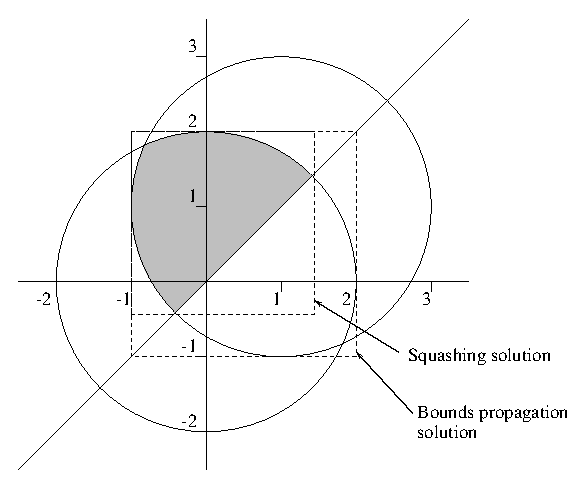
\includegraphics{squash2.eps}}
\end{center}
\caption{Example of propagation using the squash algorithm}
\label{squashfig}
\end{figure}

\begin{quote}\begin{verbatim}
?- 4 $>= X^2 + Y^2, 4 $>= (X-1)^2 + (Y-1)^2, Y $>= X.
Y = Y{-1.0000000000000004 .. 2.0000000000000004}
X = X{-1.0000000000000004 .. 2.0000000000000004}
There are 13 delayed goals.
Yes
\end{verbatim}\end{quote}

Calling \bipref{squash/3}{../bips/lib/ic/squash-3.html} results in the
bounds being tightened (in this case the bounds are tight for the feasible
region, though this is not true in general):

\begin{quote}\begin{verbatim}
?- 4 $>= X^2 + Y^2, 4 $>= (X-1)^2 + (Y-1)^2, Y $>= X,
   squash([X, Y], 1e-5, lin).
X = X{-1.0000000000000004 .. 1.4142135999632601}
Y = Y{-0.41421359996326 .. 2.0000000000000004}
There are 13 delayed goals.
Yes
\end{verbatim}\end{quote}

\See{For more details, see the IC chapter of the Library Manual or the
documentation for the individual predicates.}


\section{A larger example}
\label{farm-example}

Consider the following problem:

\begin{quote}
George is contemplating buying a farm which is a very strange shape,
comprising a large triangular lake with a square field on each side.  The
area of the lake is exactly seven acres, and the area of each field is an
exact whole number of acres.  Given that information, what is the smallest
possible total area of the three fields?
\end{quote}

A diagram of the farm is shown in Figure~\ref{lake-fields}.

\begin{figure}
\begin{center}
%\epsfbox{lake-fields.eps}
\resizebox{0.37\textwidth}{!}{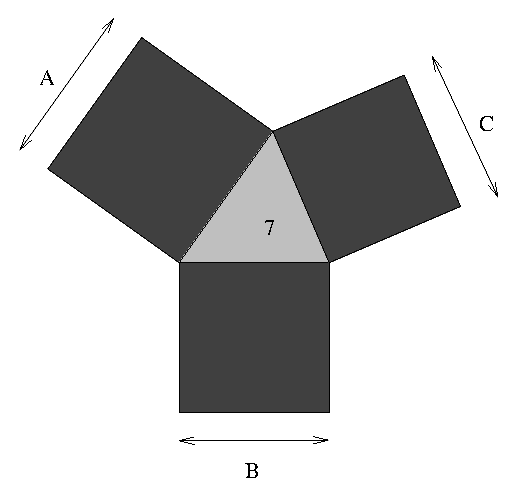
\includegraphics{lake-fields.eps}}
\end{center}
\caption{Triangular lake with adjoining square fields}
\label{lake-fields}
\end{figure}

This is a problem which mixes both integer and real quantities, and as such
is ideal for solving with the IC library.  A model for the problem appears
below.  The \texttt{farm/4} predicate sets up the constraints between the
total area of the farm \texttt{F} and the lengths of the three sides of the
lake, \texttt{A}, \texttt{B} and \texttt{C}.

\begin{code}
:- lib(ic).

farm(F, A, B, C) :-
        [A, B, C] :: 0.0 .. 1.0Inf,     % The 3 sides of the lake
        triangle_area(A, B, C, 7),      % The lake area is 7

        [F, FA, FB, FC] :: 1 .. 1.0Inf, % The square areas are integral
        square_area(A, FA),
        square_area(B, FB),
        square_area(C, FC),
        F #= FA+FB+FC,

        FA $>= FB, FB $>= FC.           % Avoid symmetric solutions

triangle_area(A, B, C, Area) :-
        S $>= 0,
        S $= (A+B+C)/2,
        Area $= sqrt(S*(S-A)*(S-B)*(S-C)).

square_area(A, Area) :-
        Area $= sqr(A).
\end{code}

A solution to the problem can then be found by first instantiating the area
of the farm, and then using \bipref{locate/2}{../bips/lib/ic/locate-2.html}
to find the lengths of the sides of the lakes.  Instantiating the area of
the farm first ensures that the first solution returned will be the minimal
one, since \bipref{indomain/1}{../bips/lib/ic/indomain-1.html} always
chooses the smallest possible value first:

\begin{code}
solve(F) :-
        farm(F, A, B, C),               % the model
        indomain(F),                    % ensure that solution is minimal
        locate([A, B, C], 0.01).
\end{code}

\section{Exercise}

\begin{enumerate}

\item

Consider the ``farm'' problem in section~\ref{farm-example}.  (Source code
may be found in \texttt{farm.ecl}, if you have access to it.) Try running
this program to find the answer.  Note that other, larger solutions are
available by selecting \emph{more}.

This implementation sums three integer variables (\texttt{FA}, \texttt{FB}
and \texttt{FC}), and then constrains their order to remove symmetries.
Would this be a good candidate for the global constraint
\texttt{ordered_sum/2}?  Modify the program so that it does use
\texttt{ordered_sum/2}.  How does the run time compare with the original?

\end{enumerate}

\index{library!ic|)}

%HEVEA\cutend

% BEGIN LICENSE BLOCK
% Version: CMPL 1.1
%
% The contents of this file are subject to the Cisco-style Mozilla Public
% License Version 1.1 (the "License"); you may not use this file except
% in compliance with the License.  You may obtain a copy of the License
% at www.eclipse-clp.org/license.
% 
% Software distributed under the License is distributed on an "AS IS"
% basis, WITHOUT WARRANTY OF ANY KIND, either express or implied.  See
% the License for the specific language governing rights and limitations
% under the License. 
% 
% The Original Code is  The ECLiPSe Constraint Logic Programming System. 
% The Initial Developer of the Original Code is  Cisco Systems, Inc. 
% Portions created by the Initial Developer are
% Copyright (C) 2006 Cisco Systems, Inc.  All Rights Reserved.
% 
% Contributor(s): 
% 
% END LICENSE BLOCK

%----------------------------------------------------------------------
\chapter{The Integer Sets Library}
\label{icsets}
\index{library!ic_sets|(}
%HEVEA\cutdef[1]{section}
%----------------------------------------------------------------------


%----------------------------------------------------------------------
\section{Why Sets}
%----------------------------------------------------------------------

\index{finite sets}
The {\em ic_sets} library is a solver for constraints over the domain
of finite sets of integers.
Modelling with sets is useful for problems where one is not
interested in each item as a specific individual, but in a
collection of item where no specific distinction is made and thus
where symmetries among the element values need to be avoided.


%----------------------------------------------------------------------
\section{Finite Sets of Integers}
%----------------------------------------------------------------------

In the context of the {\em ic_sets} library, (ground) integer sets are
simply sorted, duplicate-free lists of integers e.g.
\begin{quote}\begin{verbatim}
SetOfThree = [1,3,7]
EmptySet = []
\end{verbatim}\end{quote}
Lists which contain non-integers, are unsorted or contain duplicates,
are not sets in the sense of this library.


%----------------------------------------------------------------------
\section{Set Variables}
\index{set variable}
%----------------------------------------------------------------------

%\subsection{Declaring}
Set variables are variables which can eventually take a ground integer
set as their value.  They are characterized by a lower bound (the set
of elements that are definitely in the set) and an upper bound (the
set of elements that may be in the set).  A set variable can be
declared as follows: 
\begin{quote}\begin{verbatim}
SetVar :: []..[1,2,3,4,5,6,7]
\end{verbatim}\end{quote}
%If the lower bound is the empty set (like in this case) this can be written as 
%\begin{verbatim}
%        SetVar subset [1,2,3,4,5,6,7]
%\end{verbatim}
If the lower bound is the empty set and the upper bound is a set of
consecutive integers, one can also declare it like
\begin{quote}\begin{verbatim}
intset(SetVar, 1, 7)
\end{verbatim}\end{quote}
which is equivalent to the above.    
\quickref{Declaring Set Variables}{
\begin{description}
\item[\biptxtrefni{?Set :: ++Lwb..++Upb}{::/2!ic_sets}{../bips/lib/ic_sets/NN-2.html}]
\index{::/2@\texttt{::/2}!ic_sets} Set is an integer set within the given bounds 
\item[\biptxtref{intset(?Set, +Min, +Max)}{intset/3}{../bips/lib/ic_sets/intset-3.html}]
         Set is a set containing numbers between Min and Max 
\item[\biptxtref{intsets(?Sets, ?N, +Min, +Max)}{intsets/4}{../bips/lib/ic_sets/intsets-4.html}]
         Sets is a list of N sets containing numbers between Min and Max 
\end{description}
}

The system prints set variables in a particular way, for instance:
\begin{quote}\begin{verbatim}
?- lib(ic_sets).
?- X :: [2,3]..[1,2,3,4].
X = X{[2, 3] \/ ([] .. [1, 4]) : _308{[2 .. 4]}}
\end{verbatim}\end{quote}
The curly brackets contain the description of the current domain
of the set variable in the form of
\begin{enumerate}
\item the lower bound of the set (values which definitely are in the set)
\item the union symbol \verb.\/.
\item the set of optional values (which may or may not be in the set)
\item a colon
\item a finite domain variable indicating the admissible cardinality for the set
\end{enumerate}


%----------------------------------------------------------------------
\section{Constraints}
%----------------------------------------------------------------------

\index{membership constraint}
\index{cardinality constraint}
The constraints that {\em ic_sets} implements are the usual relations
over sets.
The membership (in/2, notin/2) and cardinality constraints
(\#/2) establish
relationships between set variables and integer variables:
\quickref{Membership and Cardinality Constraints}{
\begin{description}
\item[\biptxtrefni{?X in ?Set}{in/2!ic_sets}{../bips/lib/ic_sets/in-2.html}]
         \index{in/2@\texttt{in/2}!ic_sets} The integer X is member of the integer set Set 
\item[\biptxtrefni{?X notin ?Set}{notin/2!ic_sets}{../bips/lib/ic_sets/notin-2.html}]
         \index{notin/2@\texttt{notin/2}!ic_sets} The integer X is not a member of the integer set Set 
%\item[\biptxtref{membership_booleans(?Set, ?BoolArr)}{membership_booleans/2!ic_sets}{../bips/lib/ic_sets/membership_booleans-2.html}]
%         BoolArr is an array of booleans describing Set 
\item[\biptxtrefni{\#(?Set, ?Card)}{\#/2!ic_sets}{../bips/lib/ic_sets/H-2.html}]
         \index{\#/2@\texttt{\#/2}!ic_sets} Card is the cardinality of the integer set Set 
\end{description}
}
\begin{quote}\begin{verbatim}
?- X ::[]..[1, 2, 3], 2 in X, 3 in X, #(X, 2).
X = [2, 3]
Yes (0.01s cpu)

?- X :: []..[1, 2, 3, 4], 3 in X, 4 notin X.
X = X{[3] \/ ([] .. [1, 2]) : _2161{1 .. 3}}
Yes (0.00s cpu)
\end{verbatim}\end{quote}
Possible constraints between two sets are equality, inclusion/subset
and disjointness:
\index{inclusion constraint}
\index{disjointness constraint}
\index{subset constraint}
\begin{quote}\begin{verbatim}
?- X subset [1, 2, 3, 4].
X = X{([] .. [1, 2, 3, 4]) : _2139{0 .. 4}}
Yes (0.00s cpu)

?- X :: []..[1, 2, 3, 4], Y :: []..[3, 4, 5, 6], X subset Y.
X = X{([] .. [3, 4]) : _2176{0 .. 2}}
Y = Y{([] .. [3, 4, 5, 6]) : _2367{0 .. 4}}
There are 4 delayed goals.
Yes (0.00s cpu)

?- X :: [2] .. [1, 2, 3, 4], Y :: [3] .. [1, 2, 3, 4], X disjoint Y.
X = X{[2] \/ ([] .. [1, 4]) : _2118{1 .. 3}}
Y = Y{[3] \/ ([] .. [1, 4]) : _2213{1 .. 3}}
There are 2 delayed goals.
Yes (0.00s cpu)
\end{verbatim}\end{quote}
\quickref{Basic Set Relations}{
\begin{description}
\item[\biptxtrefni{?Set1 sameset ?Set2}{sameset/2!ic_sets}{../bips/lib/ic_sets/sameset-2.html}]
         \index{sameset/2@\texttt{sameset/2}!ic_sets} The sets Set1 and Set2 are equal 
\item[\biptxtrefni{?Set1 disjoint ?Set2}{disjoint/2!ic_sets}{../bips/lib/ic_sets/disjoint-2.html}]
         \index{disjoint/2@\texttt{disjoint/2}!ic_sets} The integer sets Set1 and Set2 are disjoint 
\item[\biptxtrefni{?Set1 includes ?Set2}{includes/2!ic_sets}{../bips/lib/ic_sets/includes-2.html}]
         \index{includes/2@\texttt{includes/2}!ic_sets} Set1 includes (is a superset) of the integer set Set2 
\item[\biptxtrefni{?Set1 subset ?Set2}{subset/2!ic_sets}{../bips/lib/ic_sets/subset-2.html}]
         \index{subset/2@\texttt{subset/2}!ic_sets} Set1 is a (non-strict) subset of the integer set Set2 
\item[\biptxtrefni{intersection(?Set1, ?Set2, ?Set3)}{intersection/3!ic_sets}{../bips/lib/ic_sets/intersection-3.html}]
         \index{intersection/3@\texttt{intersection/3}!ic_sets} Set3 is the intersection of the integer sets Set1 and Set2 
\item[\biptxtrefni{union(?Set1, ?Set2, ?Set3)}{union/3!ic_sets}{../bips/lib/ic_sets/union-3.html}]
         \index{union/3@\texttt{union/3}!ic_sets} Set3 is the union of the integer sets Set1 and Set2 
\item[\biptxtrefni{difference(?Set1, ?Set2, ?Set3)}{difference/3!ic_sets}{../bips/lib/ic_sets/difference-3.html}]
         Set3 is the difference of the integer sets Set1 and Set2 
\item[\biptxtrefni{symdiff(?Set1, ?Set2, ?Set3)}{symdiff/3!ic_sets}{../bips/lib/ic_sets/symdiff-3.html}]
         \index{symdiff/3@\texttt{symdiff/3}!ic_sets} Set3 is the symmetric difference of the integer sets Set1 and Set2 
\end{description}
}
Possible constraints between three sets are for example
intersection, union, difference and symmetric difference.
For example:
\begin{quote}\begin{verbatim}
?- X :: [2, 3] .. [1, 2, 3, 4],
   Y :: [3, 4] .. [3, 4, 5, 6],
   ic_sets : intersection(X, Y, Z).
X = X{[2, 3] \/ ([] .. [1, 4]) : _2127{2 .. 4}}
Y = Y{[3, 4] \/ ([] .. [5, 6]) : _2222{2 .. 4}}
Z = Z{[3] \/ ([] .. [4]) : _2302{[1, 2]}}
There are 6 delayed goals.
Yes (0.00s cpu)
\end{verbatim}\end{quote}
\Note{Note that we needed to qualify the intersection/3 constraint with
the {\em ic_sets} module prefix because of a name conflict with a predicate from
the {\em lists} library of the same name.}
\Note{Note the lack of a complement constraint: this is because the complement
of a finite set is infinite and cannot be represented. Complements can be
modelled using an explicit universal set and a difference constraint.}

\ignore{
\subsection{Domain Access}

\begin{description}
\item[\biptxtref{potential_members(?Set, -List)}{potential_members/2}{../bips/lib/ic_sets/potential_members-2.html}]
         List is the list of elements of whose membership in Set is currently uncertain 
\item[\biptxtref{set_range(?Set, -Lwb, -Upb)}{set_range/3}{../bips/lib/ic_sets/set_range-3.html}]
         Lwb and Upb are the current lower and upper bounds on Set 
\end{description}
}

Finally, there are a number of n-ary constraints that apply to lists of sets:
disjointness, union and intersection. For example:
\quickref{N-ary Set Relations}{
\begin{description}
\item[\biptxtref{all_disjoint(+Sets)}{all_disjoint/1}{../bips/lib/ic_sets/all_disjoint-1.html}]
         Sets is a list of integers sets which are all disjoint 
\item[\biptxtref{all_union(+Sets, ?SetUnion)}{all_union/2}{../bips/lib/ic_sets/all_union-2.html}]
         SetUnion is the union of all the sets in the list Sets 
\item[\biptxtref{all_intersection(+Sets, ?SetIntersection)}{all_intersection/2}{../bips/lib/ic_sets/all_intersection-2.html}]
         SetIntersection is the intersection of all the sets in the list Sets 
\end{description}
}
\begin{quote}\begin{verbatim}
?- intsets(Sets, 5, 1, 5), all_intersection(Sets, Common).
Sets = [_2079{([] .. [1, 2, 3, 4, 5]) : _2055{0 .. 5}}, ... ]
Common = Common{([] .. [1, 2, 3, 4, 5]) : _3083{0 .. 5}}
There are 24 delayed goals.
Yes (0.00s cpu)
\end{verbatim}\end{quote}



%----------------------------------------------------------------------
%\section{Set Expressions}
%----------------------------------------------------------------------

In most positions where a set or set variable is expected one can also
use a set expression. A set expression is composed from ground sets
(integer lists), set variables, and the following set operators:
\begin{quote}\begin{verbatim}
Set1 /\ Set2       % intersection
Set1 \/ Set2       % union
Set1 \ Set2        % difference
\end{verbatim}\end{quote}
When such set expressions occur, they are translated into auxiliary
\bipref{intersection/3}{../bips/lib/ic_sets/intersection-3.html},
\bipref{union/3}{../bips/lib/ic_sets/union-3.html} and
\bipref{difference/3}{../bips/lib/ic_sets/difference-3.html}
constraints, respectively.


%----------------------------------------------------------------------
\section{Search Support}
%----------------------------------------------------------------------

The
\bipref{insetdomain/4}{../bips/lib/ic_sets/insetdomain-4.html}
predicate can be used to enumerate all ground instantiations of a set
variable, much like
\bipref{indomain/1}{../bips/lib/ic/indomain-1.html}
in the finite domain case. 
Here is an example of the default enumeration strategy:
\begin{quote}\begin{verbatim}
?-  X::[]..[1,2,3], insetdomain(X,_,_,_), writeln(X), fail.
[1, 2, 3]
[1, 2]
[1, 3]
[1]
[2, 3]
[2]
[3]
[]
\end{verbatim}\end{quote}
Other enumeration strategies can be selected (see the Reference Manual
on insetdomain/4).


%\begin{description}
%\item[\biptxtref{insetdomain(?Set, ?CardSel, ?ElemSel, ?Order)}{insetdomain/4}{../bips/lib/ic_sets/insetdomain-4.html}]
%         Instantiate Set to a possible value 
%\end{description}


%----------------------------------------------------------------------
\section{Example}
%----------------------------------------------------------------------

\index{Steiner problem}
The following program computes so-called Steiner triplets.
The problem is to compute triplets of numbers between 1 and N,
such that any two triplets have at most one element in common.
\begin{code}
:- lib(ic_sets).
:- lib(ic).

steiner(N, Sets) :-
        NB is N * (N-1) // 6,           % compute number of triplets
        intsets(Sets, NB, 1, N),        % initialise the set variables
        ( foreach(S,Sets) do
            #(S,3)                      % constrain their cardinality
        ),
        ( fromto(Sets,[S1|Ss],Ss,[]) do
            ( foreach(S2,Ss), param(S1) do
                #(S1 /\verb.\. S2, C),         % constrain the cardinality
                C #=< 1                 % of pairwise intersections
            )
        ),
        label_sets(Sets).               % search

label_sets([]).
label_sets([S|Ss]) :-
        insetdomain(S,_,_,_),
        label_sets(Ss).
\end{code}
Running this program yields the following first solution:
\begin{quote}\begin{verbatim}
?- steiner(9,X).

X = [[1, 2, 3], [1, 4, 5], [1, 6, 7], [1, 8, 9],
     [2, 4, 6], [2, 5, 8], [2, 7, 9], [3, 4, 9],
     [3, 5, 7], [3, 6, 8], [4, 7, 8], [5, 6, 9]] More? (;)
\end{verbatim}\end{quote}


%----------------------------------------------------------------------
\section{Weight Constraints}
\label{weight-constraint}
\index{weight constraint}
%----------------------------------------------------------------------

\index{knapsack}
\index{bin packing}
Another constraint between sets and integers is the weight/3 constraint.
It allows the association of weights to set elements, and can help when
solving problems of the knapsack or bin packing type.
The constraint takes a set and an array of element weights and
constrains the weight of the whole set:
\begin{quote}\begin{verbatim}
?- ic_sets:(Container :: [] .. [1, 2, 3, 4, 5]),
   Weights = [](20, 34, 9, 12, 19),
   weight(Container, Weights, W).
Container = Container{([] .. [1, 2, 3, 4, 5]) : _2127{0 .. 5}}
Weights = [](20, 34, 9, 12, 19)
W = W{0 .. 94}
There is 1 delayed goal.
Yes (0.01s cpu)
\end{verbatim}\end{quote}
By adding a capacity limit and a search primitive, we can solve a
knapsack problem:
\begin{quote}\begin{verbatim}
?- ic_sets:(Container :: [] .. [1, 2, 3, 4, 5]),
   Weights = [](20, 34, 9, 12, 19),
   weight(Container, Weights, W),
   W #=< 50,
   insetdomain(Container,_,_,_).
Weights = [](20, 34, 9, 12, 19)
W = 41
Container = [1, 3, 4]
More (0.00s cpu)
\end{verbatim}\end{quote}

By using the heuristic options provided by insetdomain, we can
implement a greedy heuristic, which finds the optimal solution
(in terms of greatest weight) straight away:
\index{greedy heuristic}
\begin{quote}\begin{verbatim}
?- ic_sets:(Container :: [] .. [1, 2, 3, 4, 5]),
   Weights = [](20, 34, 9, 12, 19),
   weight(Container, Weights, W),
   W #=< 50,
   insetdomain(Container,decreasing,heavy_first(Weights),_).
W = 48
Container = [1, 3, 5]
Weights = [](20, 34, 9, 12, 19)
More (0.00s cpu)
\end{verbatim}\end{quote}
\quickref{Set Weight Constraint}{
\begin{description}
\item[\biptxtref{weight(?Set, ++ElementWeights, ?Weight)}{weight/3}{../bips/lib/ic_sets/weight-3.html}]
         According to the array of element weights, the weight of set Set1 is Weight 
\end{description}
}


\section{Exercises}

\begin{enumerate}

\item

Consider the knapsack problem in section~\ref{weight-constraint}.
Suppose that the items each have an associated profit, namely 17, 38, 18, 10
and 5, respectively.  Which items should be included to maximise profit?


\item

Write a predicate which, given a list of sizes of items and a list of
capacities of buckets, returns a list of (ground) sets indicating which
items should go into each bucket.  Obviously each item should go into
exactly one bucket.

Try it out with 5 items of sizes 20, 34, 9, 12 and 19, into 3 buckets of
sizes 60, 20 and 20.

\end{enumerate}

\index{library!ic_sets|)}

%HEVEA\cutend

% BEGIN LICENSE BLOCK
% Version: CMPL 1.1
%
% The contents of this file are subject to the Cisco-style Mozilla Public
% License Version 1.1 (the "License"); you may not use this file except
% in compliance with the License.  You may obtain a copy of the License
% at www.eclipse-clp.org/license.
% 
% Software distributed under the License is distributed on an "AS IS"
% basis, WITHOUT WARRANTY OF ANY KIND, either express or implied.  See
% the License for the specific language governing rights and limitations
% under the License. 
% 
% The Original Code is  The ECLiPSe Constraint Logic Programming System. 
% The Initial Developer of the Original Code is  Cisco Systems, Inc. 
% Portions created by the Initial Developer are
% Copyright (C) 2006 Cisco Systems, Inc.  All Rights Reserved.
% 
% Contributor(s): 
% 
% END LICENSE BLOCK
%
% $Id: modelling.tex,v 1.1 2006/09/23 01:49:52 snovello Exp $
%

%----------------------------------------------------------------------
\chapter{Problem Modelling}
%HEVEA\cutdef[1]{section}
%----------------------------------------------------------------------


%----------------------------------------------------------------------
\section{Constraint Logic Programming}
%----------------------------------------------------------------------

\index{Constraint Logic Programming}
\index{modelling}
One of the main ambitions of Constraint Programming is the
separation of Modelling, Algorithms and Search.
This is best characterised by two pseudo-equations.
\index{Kowalski}
The first one is paraphrased from Kowalski \cite{kowalski79}
\begin{quote}\begin{verbatim}
Solution = Logic + Control
\end{verbatim}\end{quote}
and states that we intend to solve a problem by
giving a logical, declarative description of the problem and
adding control information that enables a computer to deduce a solution.

\index{combinatorial problems}
The second equation
\begin{quote}\begin{verbatim}
Control = Reasoning + Search
\end{verbatim}\end{quote}
is motivated by a fundamental difficulty we face when dealing with
combinatorial problems: we do not have efficient algorithms
for finding solutions, we have to resort to a combination of
reasoning (via efficient algorithms) and (inefficient) search.

We can consider every constraint program as an exercise in
combining the 3 ingredients:
\begin{itemize}
\item {\bf Logic} -  The design of a declarative {\em Model} of the problem.
\item {\bf Reasoning} - The choice of clever {\em Constraint Propagation}
    algorithms that reduce the need for search.
\item {\bf Search} - The choice of search {\em strategies and heuristics} for
    finding solutions quickly.
\end{itemize}
In this chapter we will focus on the first issue, {\bf Problem Modelling},
and how it is supported by \eclipse{}.


%----------------------------------------------------------------------
\section{Issues in Problem Modelling}
%----------------------------------------------------------------------

A good formalism for problem modelling should fulfil the following criteria:
\begin{itemize}
\item {\bf Expressive power} - 
        Can we write a formal model of the real world problem?
\item {\bf Clarity for humans} - 
        How easily can the model be written, read, understood or modified?
\item {\bf Solvability for computers} - 
        Are there good known methods to solve it?
\end{itemize}
%In \eclipse{}, we model problems using a high-level logic-based language.
Higher-level models are typically
closer to the user and close to the problem and therefore
easier to understand and to trust,
easier to debug and to verify,
and easier to modify when customers change their mind.
On the other hand, it is not necessarily easy to see how they can be
solved, because high-level models contain
high-level notions (e.g.\ sets, tasks) and
heterogeneous constraints.

The constraint programming approach also addresses one of the classical
sources of error in application development with
traditional programming languages: the transition from a
{\em formal description}
of the problem to the {\em final program} that solves it.
%\begin{itemize}
%\item  Informal specification, which leads to a
%\item  Formal description, which leads to a
%\item  Program
%\end{itemize}
The question is: Can the final program be trusted?
The Constraint (Logic) Programming solution is to
\begin{itemize}
\item   Keep the initial formal model as part of the final program
\item   Enhance rather than rewrite
\end{itemize}
The process of enhancing the initial formal model involves for example
\begin{itemize}
\item Adding control annotations, e.g.
    algorithmic information or heuristic information.
\item Transformation:
    Mapping high-level (problem) constraints into
    low-level (solver) constraints,
    possibly exploiting multiple, redundant mappings.
\end{itemize}
There are many other approaches to problem modelling software.
The following is a brief comparison:
\begin{description}
\item[Formal specification languages (e.g. Z, VDM)]
    \index{specification languages}
    More expressive power than ECLiPSe, but not executable
\item[Mathematical modelling languages (e.g. OPL, AMPL)]
    \index{mathematical modelling languages}
    Similar to ECLiPSe, but usually limited expressive power,
    e.g.\ fixed set of constraints.
\item[Mainstream programming languages (e.g. C++ plus solver library)]
    \index{C++}
    Variables and constraints are "aliens" in the language.
    Specification is mixed with procedural control.
\item[Other CLP/high-level languages (e.g. CHIP)]
    \index{CHIP}
    Most similar to ECLiPSe. Less support for hybrid problem solving.
    Harder to define new constraints.
\end{description}



\section{Modelling with CLP and \eclipse{}}

When modelling problems with constraints, the basic idea is to set up
a network of variables and constraints. Figure \ref{figconsnet} shows
such a constraint network.
\begin{figure}
\begin{center}
\resizebox{0.7\textwidth}{!}{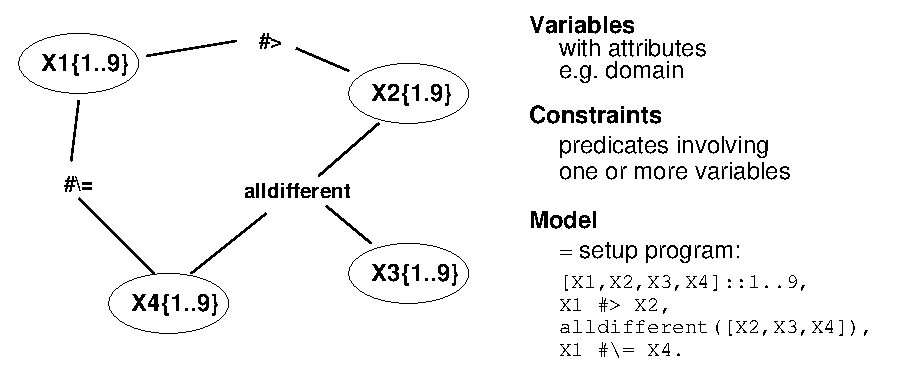
\includegraphics{consnet.eps}}
\end{center}
\caption{A Constraint Network}
\label{figconsnet}
\end{figure}
It can be seen that the Constraint Logic Programming (CLP) formulation
\begin{itemize}
\item is a natural declarative description of the constraint network
\item can serve as a program to set up the constraint network
\end{itemize}
\ignore{
The following properties make CLP langauges like
\eclipse[] suited as a modelling language:
\begin{description}
\item[Simple language]
    Logical variables,
    logical connectives (and, or, implication),
    predicates (relations, constraints),
    a single compound data type (structure),
    symbolic equality (unification)
\item[Logical reading]
        {\tt Program = Logic + Control}
\item[Flexible syntax]
        {\tt TaskA uses ResourceB}
\item[Symbolic and meta-programming capability]
        Easy to add domain-specific language features
\end{description}
}
The main \eclipse{} language constructs used in modelling are
\begin{description}
\item[Built-in constraints]\ \\
    \verb?X #> Y?
\item[Abstraction]\ \\
    \verb?before(task(Si,Di), task(Sj,Dj)) :- Si+Di #<= Sj.?
\item[Conjunction]\ \\
    \verb?between(X,Y,Z) :- X #< Y, Y #< Z.?
\item[Disjunction (but see below)]\ \\
    \verb?neighbour(X,Y) :- ( X #= Y+1 ; Y #= X+1 ).?
\item[Iteration]\ \\
    \verb?not_among(X, L) :- ( foreach(Y,L),param(X) do X #\= Y ).?
\item[Recursion]\ \\
    \verb?not_among(X, []).?\\
    \verb?not_among(X, [Y|Ys]) :- X #\= Y, not_among(X, Ys).?
\end{description}


%----------------------------------------------------------------------
\section{Same Problem - Different Model}
%----------------------------------------------------------------------

There are often many ways of modelling a problem.
Consider the famous "SEND + MORE = MONEY" example:
\begin{code}
sendmore(Digits) :-
    Digits = [S,E,N,D,M,O,R,Y],
    Digits :: [0..9],
    alldifferent(Digits),
    S #\verb.\.= 0, M #\verb.\.= 0,
                 1000*S + 100*E + 10*N + D
               + 1000*M + 100*O + 10*R + E
    #= 10000*M + 1000*O + 100*N + 10*E + Y.
\end{code}
An alternative model is based on the classical decimal addition algorithm with
carries:
\begin{code}
sendmore(Digits) :-
    Digits = [S,E,N,D,M,O,R,Y],
    Digits :: [0..9],
    Carries = [C1,C2,C3,C4],
    Carries :: [0..1],
    alldifferent(Digits),
    S #\verb.\.= 0,
    M #\verb.\.= 0,
    C1         #= M,
    C2 + S + M #= O + 10*C1,
    C3 + E + O #= N + 10*C2,
    C4 + N + R #= E + 10*C3,
         D + E #= Y + 10*C4.
\end{code}
Both models work fine, but obviously involve different variables and
constraints. Even though high-level models reduce the need for finding
sophisticated encodings of problems, finding good models still requires
substantial expertise and experience.

\ignore{
Abstraction

:- lib(ria).                            % Using interval library

farm(F) :-
        [A,B,C] :: 0.0..inf,            % The 3 sides of the lake
        triangle_area(A, B, C, 7),      % The lake area is 7

        [F,FA,FB,FC] :: 1..inf,         % The square areas are integral
        square_area(A, FA),
        square_area(B, FB),
        square_area(C, FC),
        F *= FA+FB+FC,

        FA *>= FB, FB *>= FC.           % Avoid symmetric solutions

triangle_area(A, B, C, Area) :-
        S *>= 0,
        S *= (A+B+C)/2,
        Area *= sqrt(S*(S-A)*(S-B)*(S-C)).

square_area(A, Area) :-
        Area *= sqr(A).
}


\ignore{
\subsection{Using Data Structures}

Structures
Task = task(plumbing, S, 3, R, _)
Task = task with [duration:3, resource:R, start:S, name:plumbing]
Lists
Digits = [S,E,N,D,M,O,R,Y]
length(VarList, 100)
Arrays
dim(ChessBoard, [8,8])
VarArray =.. [_|VarList]

In ECLiPSe, lists and arrays are just special structures!
}



\section{Rules for Modelling Code}

In CLP, the declarative model is at the same time the constraint setup code.
This code should therefore be deterministic and terminating, so:
\begin{description}
\item[Careful with disjunctions]
    Don't leave choice-points (alternatives for backtracking).
    Choices should be deferred until search phase.
\item[Use only simple conditionals]
    Conditions in \verb=(...->...;...)= must be true or false at modelling time!
\item[Use only structural recursion and loops]
    Termination conditions must be know at modelling time!
\end{description}

\subsection{Disjunctions}

Disjunctions in the model should be avoided. Assume that a naive
model would contain the following disjunction:
\begin{code}
% DO NOT USE THIS IN A MODEL
no_overlap(S1,D1,S2,D2) :- S1 #>= S2 + D2.
no_overlap(S1,D1,S2,D2) :- S2 #>= S1 + D1.
\end{code}
There are two basic ways of treating the disjunction:
\begin{itemize}
\item Deferring the choice until the search phase by introducing a
        decision variable.
\item Changing the behaviour of the disjunction so it becomes a constraint
        (see also \ref{chapimpl} and \ref{chappropiachr}).
\end{itemize}
In the example, we can introduce a boolean variable \verb.B{0,1}. which represents
the choice.
The actual choice can be then be taken in search code by choosing a
value for the variable. The model code must then be changed to observe
the decision variable, either using the delay facility of \eclipse{}:
\begin{code}
delay no_overlap(S1,D1,S2,D2,B) if var(B).
no_overlap(S1,D1,S2,D2,0) :- S1 #>= S2 + D2.
no_overlap(S1,D1,S2,D2,1) :- S2 #>= S1 + D1.
\end{code}
or using an arithmetic encoding like in
\begin{code}
no_overlap(S1,D1,S2,D2,B) :-
        B :: 0..1, 
        S1 +     B*1000 #>= S2 + D2,
        S2 + (1-B)*1000 #>= S1 + D1.
\end{code}
The alternative of turning the disjunction into a proper constraint is
achieved most easily using {\em propia}'s infer-annotation
(see \ref{chappropiachr}). The original formulation of neighbour/2
is kept but it is used as follows:
\begin{code}
    ..., no_overlap(S1,D2,S2,D2) infers most, ...
\end{code}


\subsection{Conditionals}

Similar considerations apply to conditionals where the condition is not
decidable at constraint setup time. For example, suppose we want to
impose a no-overlap constraint only if two tasks share the same resource.
The following code is currently not safe in ECLiPSe:
\begin{code}
nos(Res1, Res2, Start1, Dur1, Start2, Dur2) :-
    ( Res1 #= Res2 ->           % WRONG!!!
        no_overlap(Start1, Dur1, Start2, Dur2)
    ;
        true
    )
\end{code}
The reason is that (at constraint setup time) Res1 and Res2 will most
likely be still uninstantiated. Therefore, the condition will in general
delay (rather than succeed or fail), but the conditional construct
will erroneously take this for a success and take the first alternative.

Again, this can be handled using delay
\begin{code}
delay nos(Res1, Res2, _, _, _, _) if nonground([Res1,Res2]).
nos(Res1, Res2, Start1, Dur1, Start2, Dur2) :-
    ( Res1 == Res2 ->
        no_overlap(Start1, Dur1, Start2, Dur2)
    ;
        true
    ).
\end{code}
It might also be possible to compute a boolean variable indicating the
truth of the condition. This is particularly easy when a reified
constraint can be used to express the condition, like in this case:
\begin{code}
nos(Res1, Res2, Start1, Dur1, Start2, Dur2) :-
    #=(Res1, Res2, Share),
    cond_no_overlap(Start1, Dur1, Start2, Dur2, Share).

delay cond_no_overlap(_,_,_,_,Share) if var(Share).
cond_no_overlap(Start1, Dur1, Start2, Dur2, Share) :-
    ( Share == 1 ->
        no_overlap(Start1, Dur1, Start2, Dur2)
    ;
        true
    ).
\end{code}


\section{Symmetries}

Consider the following puzzle, where numbers from 1 to 19 have to be arranged
in a hexagonal shape such that every diagonal sums up to 38:
\begin{code}
puzzle(Pattern) :-
        Pattern = [
                   A,B,C,
                  D,E,F,G,
                 H,I,J,K,L,
                  M,N,O,P,
                   Q,R,S
                  ],
        Pattern :: 1 .. 19,

        % Problem constraints
        alldifferent(Pattern),
          A+B+C #= 38,     A+D+H #= 38,     H+M+Q #= 38,
         D+E+F+G #= 38,   B+E+I+M #= 38,   D+I+N+R #= 38,
        H+I+J+K+L #= 38, C+F+J+N+Q #= 38, A+E+J+O+S #= 38,
         M+N+O+P #= 38,   G+K+O+R #= 38,   B+F+K+P #= 38,
          Q+R+S #= 38,     L+P+S #= 38,     C+G+L #= 38,
        ...
\end{code}
In this formulation, the problem has 12 solutions, but it turns out they
are just rotated and mirrored variants of each other.
Removal of symmetries is still an area of active research, but a simple
method is applicable in situations like this one.
One can add constraints which require the solution to have certain
additional properties, and so exclude many of the symmetric solutions:
\begin{code}
        ...,
        % Optional anti-symmetry constraints
        % Forbid rotated solutions: require A to be the smallest corner
        A #< C, A #< H, A #< L, A #< S, A #< Q,
        % Forbid solutions mirrored on the A-S diagonal
        C #< H.
\end{code}

%HEVEA\cutend

% BEGIN LICENSE BLOCK
% Version: CMPL 1.1
%
% The contents of this file are subject to the Cisco-style Mozilla Public
% License Version 1.1 (the "License"); you may not use this file except
% in compliance with the License.  You may obtain a copy of the License
% at www.eclipse-clp.org/license.
% 
% Software distributed under the License is distributed on an "AS IS"
% basis, WITHOUT WARRANTY OF ANY KIND, either express or implied.  See
% the License for the specific language governing rights and limitations
% under the License. 
% 
% The Original Code is  The ECLiPSe Constraint Logic Programming System. 
% The Initial Developer of the Original Code is  Cisco Systems, Inc. 
% Portions created by the Initial Developer are
% Copyright (C) 2006 Cisco Systems, Inc.  All Rights Reserved.
% 
% Contributor(s): 
% 
% END LICENSE BLOCK

%\documentclass[11pt,a4paper]{book}
%\usepackage{alltt}
%\usepackage{graphics}
%%\usepackage{html}
%\topmargin 0cm
%\oddsidemargin 0cm
%\evensidemargin 0cm
%\textwidth 16cm
%\textheight 22.5cm
%
%% Allow underscores as normal characters (but lose subscripts...)
%% [moved into include file because of latex2html problem]
%%\catcode`_=\active
%
%\def\eclipse{ECL$^i$PS$^e$}
%
%% Don't use a style file for sepiachip because latex2html ignores it
%
%\makeindex
%
%\begin{document}
%
%\title{{\huge Search in ECLiPSe}}
%\author{Joachim Schimpf \and Kish Shen \and Mark Wallace}
%
%\maketitle
%%\abstract{
%%This tutorial is an overwiew of different search methods to Prolog,
%%and how to implement them in ECLiPSe.
%%}
%
%\tableofcontents

%\chapter{Search Methods}
%----------------------------------------------------------------------
\section{Introduction}
%----------------------------------------------------------------------
In this tutorial we will take a closer look at the principles and
alternative methods of searching for solutions in the presence of
constraints. Let us first recall what we are talking about.
We assume we have the standard pattern of a constraint program:
\begin{quote}\begin{alltt}
solve(Data) :-
        model(Data, Variables),
        search(Variables),
        print_solution(Variables).
\end{alltt}\end{quote}
The model part contains the logical {\em model} of our problem. It defines
the variables and the constraints.
Every variable has a {\em domain} of values that it can take
(in this context, we only consider domains with a finite number of values).

Once the model is set up, we go into the search phase.
Search is necessary since generally the implementation of the constraints
is not complete, i.e.\ not strong enough to logically infer directly
the solution to the problem. Also, there may be multiple solutions
which have to be located by search, e.g.\ in order to find the best one.
In the following, we will use the following terminology:
\begin{itemize}
\item If a variable is given a value (from its domain, of course),
        we call this an {\em assignment}. If every problem variable is given
        a value, we call this a {\em total assignment}.
\item A total assignment is a {\em solution} if it satisfies all the
        constraints.
\item The {\em search space} is the set of all possible total assignments.
        The search space is usually very large because it grows exponentially
        with the problem size:
        \begin{displaymath}
        SearchSpaceSize = {DomainSize}^{NumberOfVariables}
        \end{displaymath}
\end{itemize}


% - - - - - - - - - - - - - - - - - - - - - - - - - - - - - - - - - - -
\subsection{Overview of Search Methods}
% - - - - - - - - - - - - - - - - - - - - - - - - - - - - - - - - - - -

\begin{figure}
\begin{center}

\includegraphics{search3.eps}
\end{center}
\caption{A search space of size 16}
\label{figsearchspace}
\end{figure}
Figure \ref{figsearchspace} shows a search space with N (here 16)
possible total assignments, some of which are solutions.
Search methods now differ in the way in which these assignments
are visited.
We can classify search methods according to different criteria:
\begin{description}
\item[Complete vs incomplete exploration] complete search means that the search space
    is investigated in such a way that all solutions are guaranteed to be found.
    This is necessary when the optimal solution is needed (one has to prove
    that no better solution exists). Incomplete search may be sufficient when
    just some solution or a relatively good solution is needed.
\item[Constructive vs move-based] this indicates whether the method advances
    by incrementally constructing assignments (thereby reasoning about partial
    assignments which represent subsets of the search space) or by moving
    between total assignments (usually by modifying previously explored
    assignments).
\item[Randomness] some methods have a random element while others follow
    fixed rules.
\end{description}
Here is table of a selection of search methods together with their properties:

\begin{center}
\begin{tabular}{|l|lll|}
\hline
Method&                 exploration&    assignments&    random\\
\hline
Full tree search&       complete&       constructive&   no\\
Credit search&          incomplete&     constructive&   no\\
Bounded backtrack&      incomplete&     constructive&   no\\
Limited discrepancy&    complete&       constructive&   no\\
Hill climbing&          incomplete&     move-based&     possibly\\
Simulated annealing&    incomplete&     move-based&     yes\\
Tabu search&            incomplete&     move-based&     possibly\\
Weak commitment&        complete&       hybrid&         no\\
\hline
\end{tabular}
\end{center}

The constructive search methods usually organise the search space by
partitioning it systematically.  This can be done naturally with a
search tree (Figure \ref{figsearchtree}).  The nodes in this tree
represent choices which partition the remaining search space into two
or more (usually mutually exclusive) disjoint sub-spaces.  Using such
a tree structure, the search space can be traversed systematically and
completely (with as little as O(N) memory requirements).

\begin{figure}
\begin{center}
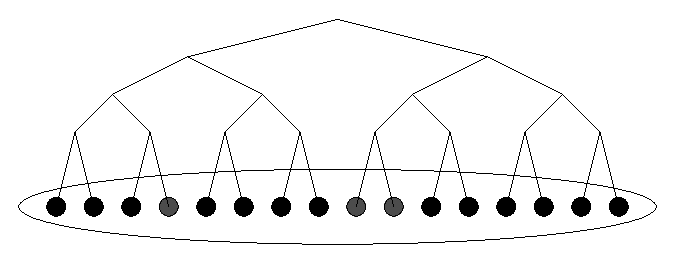
\includegraphics{search4.eps}
\end{center}
\caption{Search space structured using a search tree}
\label{figsearchtree}
\end{figure}
Figure \ref{figtreesearch} shows a sample tree search, namely a depth-first
incomplete traversal.
As opposed to that, figure \ref{figmovesearch} shows an example of an
incomplete move-based search which does not follow a fixed search space
structure. Of course, it will have to take other precautions to avoid
looping and ensure termination.
\begin{figure}
\begin{center}

\includegraphics{search5.eps}
\end{center}
\caption{A move-based search}
\label{figmovesearch}
\end{figure}

\begin{figure}
\begin{center}
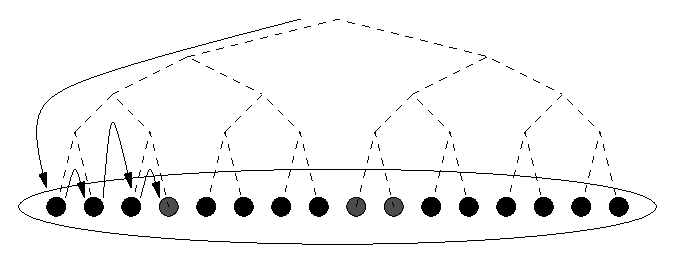
\includegraphics{search6.eps}
\end{center}
\caption{A tree search (depth-first)}
\label{figtreesearch}
\end{figure}

A few further observations:
Move-based methods are usually incomplete. This is not surprising given
typical sizes of search spaces.
A complete exploration of a huge search space
is only possible if large sub-spaces can be excluded a priory, and this
is only possible with constructive methods which allow to reason about
whole classes of similar assignments.
Moreover, a complete search method must remember which parts of the
search space have already been visited.
This can only be implemented with
acceptable memory requirements if there is a simple structuring of the
space that allows compact encoding of sub-spaces.


% - - - - - - - - - - - - - - - - - - - - - - - - - - - - - - - - - - -
\subsection{Optimisation and Search}
% - - - - - - - - - - - - - - - - - - - - - - - - - - - - - - - - - - -

Many practical problems are in fact optimisation problems, ie.\ we are
not just interested in some solution or all solutions, but in
the best solution.

Fortunately, there is a general method to find the optimal solution
based on the ability to find all solutions.
\index{branch-and-bound}
The {\em branch-and-bound} technique works are follows:
\begin{enumerate}
\item Find a first solution
\item Add a constraint requiring a better solution than the best
    one we have so far (e.g.\ require lower cost)
\item Find a solution which satisfies this new constraint.
    If one exists, we have a new best solution and we repeat step 2.
    If not, the last solution found is the proven optimum.
\end{enumerate}
The library {\bf branch\_and\_bound} provides the generic
branch-and-bound primitives bb\_min/3 and bb\_min/6.


% - - - - - - - - - - - - - - - - - - - - - - - - - - - - - - - - - - -
\subsection{Heuristics}
% - - - - - - - - - - - - - - - - - - - - - - - - - - - - - - - - - - -

Since search space sizes grow exponentially with problem size,
it is not possible to explore all assignments except for the
very smallest problems.
The only way out is {\em not} to look at the whole search space.
There are only two ways to do this:
\begin{itemize}
\item {\bf Prove} that certain areas of the space contain no solutions.
    This can be done with the help of constraints. This is often referred
    to as {\em pruning}\index{pruning}.
\item {\bf Ignore} parts of the search space that are unlikely to contain
    solutions (i.e.\ do incomplete search), or at least postpone their exploration.
    This is done by using {\em heuristics}\index{heuristics}.
    A heuristic is a particular traversal order of the search space
    which explores promising areas first.
\end{itemize}

In the following sections we will first investigate the considerable
degrees of freedom that are available for heuristics within the framework of
systematic tree search, which is the traditional search method
in the Constraint Logic Programming world.

Subsequently, we will turn our attention to move-based methods
which in {\eclipse} can be implemented using the facilities of the repair-library.


%----------------------------------------------------------------------
\section{Complete Tree Search with Heuristics}
%----------------------------------------------------------------------

There is one form of tree search which is especially economic: 
depth-first, left-to-right search by backtracking.  It allows to
traverse a search tree systematically while requiring only a stack
of maximum depth N for bookkeeping.  Most other strategies of tree
search (e.g.  breadth-first) have exponential memory requirements. 
This unique property is the reason why backtracking is a built feature
of {\eclipse}.  Note that the main disadvantage of the depth-first
strategy (the danger of going down an infinite branch) does not come
into play here because we deal with finite search trees.

Sometimes depth-first search and heuristic search are treated as antonyms.
This is only justified when the shape of the search tree is statically fixed.
Our case is different: we have the freedom of deciding on the shape of every
sub-tree before we start to traverse it depth-first. While this does not
allow to arrange for {\em any} order of visiting the leaves of the search tree,
it does provide considerable flexibility. This flexibility can be exploited
by variable and value selection strategies.

% - - - - - - - - - - - - - - - - - - - - - - - - - - - - - - - - - - -
\subsection{Search Trees}
% - - - - - - - - - - - - - - - - - - - - - - - - - - - - - - - - - - -

In general, the nodes of a search tree represent {\em choices}.
\index{choice}
These choices should be mutually exclusive and therefore partition the
\index{partition a search space}
search space into two or more disjoint sub-spaces.
In other words, the original problem is reduced to a disjunction
of simpler sub-problems.

In the case of finite-domain problems, the most common form of choice
is to choose a particular value for a problem variable
(this technique is often called
\index{labeling}
{\em labeling}).
For a boolean variable, this means setting the variable to 0 in one
branch of the search tree and to 1 in the other.
In {\eclipse}, this can be written as a disjunction
(which is implemented by backtracking):
\begin{quote}\begin{alltt}
( X1=0 ; X1=1 )
\end{alltt}\end{quote}
Other forms of choices are possible. If X2 is a variable that can take
integer values from 0 to 3 (assume it has been declared as \verb'X2::0..3'),
we can make a n-ary search tree node by writing
\begin{quote}\begin{alltt}
( X2=0 ; X2=1 ; X2=2 ; X2=3 )
\end{alltt}\end{quote}
or more compactly
\begin{quote}\begin{alltt}
indomain(X2)
\end{alltt}\end{quote}
However, choices do not necessarily involve choosing a concrete value
for a variable. It is also possible to make disjoint choices by
\index{domain splitting}
{\em domain splitting}, e.g.
\begin{quote}\begin{alltt}
( X2 #=< 1 ; X2 #>= 2 )
\end{alltt}\end{quote}
or by choosing a value in one branch and excluding it in the other:
\begin{quote}\begin{alltt}
( X2 = 0 ; X2 #>= 1 )
\end{alltt}\end{quote}
In the following examples, we will mainly use simple labeling,
which means that the search tree nodes correspond to a variable
and a node's branches correspond to the different values that the
variable can take.


% - - - - - - - - - - - - - - - - - - - - - - - - - - - - - - - - - - -
\subsection{Variable Selection}
% - - - - - - - - - - - - - - - - - - - - - - - - - - - - - - - - - - -

\begin{figure}
\begin{center}
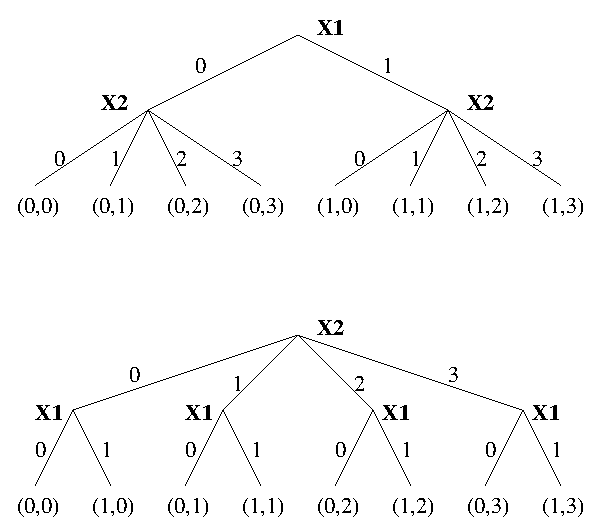
\includegraphics{search1.eps}
\end{center}
\caption{The effect of variable selection}
\label{figvarsel}
\end{figure}

Figure \ref{figvarsel} shows how variable selection reshapes a search tree.
If we decide to choose values for X1 first (at the root of the search tree)
and values for X2 second, then the search tree has one particular shape.
If we now assume a depth-first, left-to-right traversal by backtracking,
this corresponds to one particular order of visiting the leaves of the tree:
(0,0), (0,1), (0,2), (0,3), (1,0), (1,1), (1,2), (1,3).

If we decide to choose values for X2 first and X1 second, then the tree and
consequently the order of visiting the leaves is different:
(0,0), (1,0), (0,1), (1,1), (0,2), (1,2), (0,3), (1,3).

While with 2 variables there are only 2 variable selection strategies,
this number grows exponentially with the number of variables. For 5
variables there are already $2^{2^{5}-1} = 2147483648$ different variable selection
strategies to choose from.

Note that the example shows something else: If the domains of the variables
are different, then the variable selection can change the number of internal
nodes in the tree (but not the number of leaves). To keep the number of nodes
down, variables with small domains should be selected first.


% - - - - - - - - - - - - - - - - - - - - - - - - - - - - - - - - - - -
\subsection{Value Selection}
% - - - - - - - - - - - - - - - - - - - - - - - - - - - - - - - - - - -

The other way to change the search tree is value selection, i.e. reordering
the child nodes of a node by choosing the 
values from the domain of a variable in a particular order.
Figure \ref{figvalsel} shows how this can change the order of visiting the
leaves:
(1,2), (1,1), (1,0), (1,3), (0,1), (0,3), (0,0), (0,2).

\begin{figure}
\begin{center}
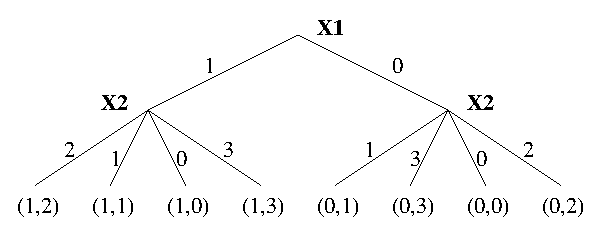
\includegraphics{search2.eps}
\end{center}
\caption{The effect of value selection}
\label{figvalsel}
\end{figure}

By combining variable and value selection, a large number of different
heuristics can be implemented.
To give an idea of the numbers involved, the following table shows the search
space sizes, the number of possible search space traversal orderings,
and the number of orderings
that can be obtained by variable and value selection (assuming domain size 2).

\enableunderscores
\begin{center}
\begin{tabular}{|l|l|l|l|}
\hline
Variables&      Search space&   Visiting orders&        Selection Strategies\\
\hline
1&              2&                      2&              2\\
2&              4&                      24&             16\\
3&              8&                      40320&          336\\
4&              16&                     $2.1*10^{13}$&  $1.8*10^7$\\
5&              32&                     $2.6*10^{35}$&  $3.5*10^{15}$\\
n&              $2^n$&          $2^n!$& 
                                $2^{{2^n}-1} \prod_{i=0}^{n-1} (n-1)^{2^i}$\\
\hline
\end{tabular}
\end{center}
\disableunderscores

% - - - - - - - - - - - - - - - - - - - - - - - - - - - - - - - - - - -
\subsection{Example}
% - - - - - - - - - - - - - - - - - - - - - - - - - - - - - - - - - - -

We use the famous N-Queens problem to illustrate how heuristics can be applied
to backtrack search through variable and value selection.
We model the problem with one variable per queen, assuming that each queen
occupies one colunm. The variables range from 1 to N and indicate the row
in which the queen is being placed. The constraints ensure that no two
queens occupy the same row or diagonal:
%!!!!!!!!!!!!!!!!!!!!!!!!!!!!!!!!!!!!!!!!!!!!!!!!!!
% CAUTION: I use the old ## syntax here because
% #\= is not treated correctly by latex2html
%!!!!!!!!!!!!!!!!!!!!!!!!!!!!!!!!!!!!!!!!!!!!!!!!!!
\begin{quote}\begin{alltt}
:- lib(fd).

queens(N, Board) :-
        length(Board, N),
        Board :: 1..N,
        ( fromto(Board, [Q1|Cols], Cols, []) do
            ( foreach(Q2, Cols), count(Dist,1,_), param(Q1) do
                noattack(Q1, Q2, Dist)
            )
        ).

    noattack(Q1,Q2,Dist) :-
        Q2 ## Q1,
        Q2 - Q1 ## Dist,
        Q1 - Q2 ## Dist.
\end{alltt}\end{quote}
We are looking for a first solution to the 16-queens problem by calling
\begin{quote}\begin{alltt}
?- queens(16, Vars),   % model
   labeling(Vars).     % search
\end{alltt}\end{quote}
We start naively, using the pre-defined labeling-predicate that comes with the
finite-domain library. It is defined as follows:
\begin{quote}\begin{alltt}
labeling(AllVars) :-
        ( foreach(Var, AllVars) do
            indomain(Var)                       % select value
        ).
\end{alltt}\end{quote}
The strategy here is simply to select the variables
from left to right as they occur in the list, and they are
assigned values starting from the lowest to the numerically highest they can
take (this is the definition of indomain/1).
A solution is found after 542 backtracks
(see section \ref{countbt} below for how to count backtracks).

A first improvement is to employ a
{\bf general-purpose variable-selection heuristic},
\index{first-fail principle}
the so called first-fail principle. It requires to label the
variables with the smallest domain first. This reduces the branching
factor at the root of the search tree and the total number of internal nodes.
The deleteff/3 predicate implements this strategy for finite domains.
Using deleteff/3, we can redefine our labeling-routine as follows:
\begin{quote}\begin{alltt}
labeling(AllVars) :-
        ( fromto(AllVars, Vars, VarsRem, []) do
            deleteff(Var, Vars, VarsRem),       % dynamic var-select
            indomain(Var)                       % select value
        ).
\end{alltt}\end{quote}
Indeed, for the 16-queens example, this leads to a dramatic improvement,
the first solution is found with only 3 backtracks now.
But caution is necessary: The 256-queens instance for example solves
nicely with the naive strategy, but our improvement leads to a
disappointment: the time increases dramatically!
This is not uncommmon with heuristics: one has to keep in mind that the
search space is not reduced, just re-shaped. Heuristics that yield good
results with some problems can be useless or counter-productive with others.
Even different instances of the same problem can exhibit widely different
characteristics.
 
Let us try to employ a {\bf problem-specific heuristic}:
Chess players know that pieces in the middle of the board are more
useful because they can attack more fields. We could therefore start
placing queens in the middle of the board to reduce the number of
unattacked fields earlier. We can achieve that simply by pre-ordering the
variables such that the middle ones are first in the list:
\begin{quote}\begin{alltt}
labeling(AllVars) :-
        middle_first(AllVars, AllVarsPreOrdered), % static var-select
        ( foreach(Var, AllVarsPreOrdered) do
            indomain(Var)                       % select value
        ).
\end{alltt}\end{quote}
The implementation of middle\_first/2 requries a bit of list manipulation
and uses primitives from the lists-library:
\begin{quote}\begin{alltt}
:- lib(lists).

middle_first(List, Ordered) :-
        halve(List, Front, Back),
        reverse(Front, RevFront),
        splice(Back, RevFront, Ordered).
\end{alltt}\end{quote}
This strategy also improves things for the 16-queens instance, the
first solution requires 17 backtracks.

We can now improve things further by {\bf combining} the two
variable-selection strategies:
When we pre-order the variables such that the middle ones are first,
the deleteff/3 predicate will prefer middle variables when several
have the same domain size:
\begin{quote}\begin{alltt}
labeling(AllVars) :-
        middle_first(AllVars, AllVarsPreOrdered), % static var-select
        ( fromto(AllVarsPreOrdered, Vars, VarsRem, []) do
            deleteff(Var, Vars, VarsRem),       % dynamic var-select
            indomain(Var)                       % select value
        ).
\end{alltt}\end{quote}
The result is positive: for the 16-queens instance,
the number of backtracks goes down to zero,
and more difficult instances become solvable!

Actually, we have not yet implemented our intuitive heuristics properly.
We start placing queens in the middle columns, but not on the middle rows.
With our model, that can only be achieved by {\bf changing the value selection},
ie.\ setting the variables to values in the middle of their domain.
We therefore invent a variant of indomain/1 called middle\_first\_indomain/1
and the resulting labeling routine then looks as follows:
\begin{quote}\begin{alltt}
labeling(AllVars) :-
        middle_first(AllVars, AllVarsPreOrdered), % static var-select
        ( fromto(AllVarsPreOrdered, Vars, VarsRem, []) do
            deleteff(Var, Vars, VarsRem),       % dynamic var-select
            middle_first_indomain(Var)          % select value
        ).
\end{alltt}\end{quote}
The implementation of middle\_first\_indomain/2
simply relies on middle\_first/2:
\begin{quote}\begin{alltt}
middle_first_indomain(X) :-
        nonvar(X).
middle_first_indomain(X) :-
        var(X),
        dom(X, List),    % the list of values in X's domain
        middle_first(List, Ordered),
        member(X, Ordered).
\end{alltt}\end{quote}
Surprisingly, this improvement again increases the backtrack count for
16-queens again to 3.
However, when looking at a number of different instances of the problem,
we can observe that the overall behaviour has improved and the
performance has become more predictable than with the
initial more naive strategies.


% - - - - - - - - - - - - - - - - - - - - - - - - - - - - - - - - - - -
\subsection{Counting Backtracks}
% - - - - - - - - - - - - - - - - - - - - - - - - - - - - - - - - - - -

%The size of the (remaining) search space can be computed easily
%in finite-domain problems. All we have to do is to multiply the
%sizes of all the (remaining) variable's domains:
%\begin{quote}\begin{alltt}
%search_space(Vars, Size) :-
%        ( foreach(V,Vars), fromto(1,S0,S1,Size) do
%            dvar_domain(V,D), S1 is S0*dom_size(D)
%        ).
%\end{alltt}\end{quote}

\label{countbt}
An interesting piece of information during program development is the
number of backtracks. It is a good measure for the quality of
both constraint propagation and search heuristics.
We can instrument our labeling routine as follows:
\begin{quote}\begin{alltt}
labeling(AllVars) :-
        init_backtracks,
        ( foreach(Var, AllVars) do
            count_backtracks,       % insert this before choice!
            indomain(Var)
        ),
        get_backtracks(B),
        printf("Solution found after %d backtracks%n", [B]).
\end{alltt}\end{quote}
The backtrack counter itself can be implemented by the code below.
It uses a non-logical counter variable (backtracks) and an additional
flag (deep\_fail) which ensures that backtracking to exhausted choices
does not increment the count.
\begin{quote}\begin{alltt}
:- local variable(backtracks), variable(deep_fail).

init_backtracks :-
        setval(backtracks,0).

get_backtracks(B) :-
        getval(backtracks,B).

count_backtracks :-
        setval(deep_fail,false).
count_backtracks :-
        getval(deep_fail,false),        % may fail
        setval(deep_fail,true),
        incval(backtracks),
        fail.
\end{alltt}\end{quote}
Note that there are other possible ways of defining the number of backtracks.
However, the one suggested here has the following useful properties:
\begin{itemize}
\item Shallow backtracking (an attempt to instantiate a variable which
    causes immediate failure due to constraint propagation) is not counted.
    If constraint propagation works well, the count is therefore zero.
\item With a perfect heuristic, the first solution is found with zero
    backtracks.
\item If there are N solutions, the best achievable value is N (one backtrack
    per solution). Higher values indicate an opportunity to improve pruning
    by constraints.
\end{itemize}


%----------------------------------------------------------------------
\section{Incomplete Tree Search}
%----------------------------------------------------------------------
%\subsection{Pruning with Extra Constraints}
%\subsection{First Solution}

% - - - - - - - - - - - - - - - - - - - - - - - - - - - - - - - - - - -
\subsection{Bounded Backtrack Search} 
% - - - - - - - - - - - - - - - - - - - - - - - - - - - - - - - - - - -

One way to limit the scope of backtrack search is to keep a
record of the number of backtracks, and curtail the search when this
limit is exceeded.

You can find an implementation of Bounded Backtrack Search ({\em BBS})
in the file {\tt lds.ecl} in the {\tt doc/examples} directory of your
{\eclipse} installation.
The predicate defining bounded backtrack search is
\verb0bounded_backtrack_search0, and it takes two arguments, a list of
variables and an integer (the limit on the number of backtracks).
An example invocation is:
\begin{quote}\begin{alltt}
?- [X,Y,Z]::1..3, X+Y+Z#=6, bounded_backtrack_search([X,Y,Z],4).
\end{alltt}\end{quote}
The answers are returned on backtracking in the following order:
\begin{itemize}
\item
X = 1
Y = 2
Z = 3
\item
X = 1
Y = 3
Z = 2  
\item
X = 2
Y = 1
Z = 3
\item
X = 2
Y = 2
Z = 2    
\end{itemize}
After which the procedure fails outputting
\verb0Backtrack limit exceeded0.

The implementation uses several
facilities of {\eclipse}, including {\em non-logical variables} and
{\em catch and throw}:
\begin{quote}\begin{alltt}
:- local variable(backtracks), variable(deep_fail).

bounded_backtrack_search(List,Limit) :-
        setval(backtracks,Limit),
        block(bbs_label(List),
              exceed_limit,
              (writeln('Backtrack limit exceeded'), fail)
             ).

bbs_label([]).
bbs_label([Var|Vars]) :-
        limit_backtracks,
        indomain(Var),
        bbs_label(Vars).
    
limit_backtracks :-
        setval(deep_fail,false).
limit_backtracks :-
        getval(deep_fail,false),        % may fail
        setval(deep_fail,true),
        decval(backtracks),
        (getval(backtracks,0) -> exit_block(exceed_limit) ; fail).
\end{alltt}\end{quote}


% - - - - - - - - - - - - - - - - - - - - - - - - - - - - - - - - - - -
\subsection{Credit Search}
% - - - - - - - - - - - - - - - - - - - - - - - - - - - - - - - - - - -

Credit search is a tree search method where the number of
nondeterministic choices is limited a priori.  This is achieved by
starting the search at the tree root with a certain integral amount of
credit.  This credit is split between the child nodes, their credit
between their child nodes, and so on.  A single unit of credit cannot
be split any further: subtrees provided with only a single credit unit
are not allowed any nondeterministics choices, only one path though these
subtrees can be explored, i.e. only one leaf in the subtree can be visited.
Subtrees for which no credit is left are pruned,
i.e.\ not visited.

The following code (a replacement for labeling/1)
implements credit search. For ease of understanding, it is
limited to boolean variables:
\begin{quote}\begin{alltt}
% Credit search (for boolean variables only)
credit_search(Credit, Xs) :-
        (
            foreach(X, Xs),
            fromto(Credit, ParentCredit, ChildCredit, _)
        do
            ( var(X) ->
                ParentCredit > 0,  % possibly cut-off search here
                ( % Choice
                    X = 0, ChildCredit is (ParentCredit+1)//2
                ;
                    X = 1, ChildCredit is ParentCredit//2
                )
            ;
                ChildCredit = ParentCredit
            )
        ).
\end{alltt}\end{quote}
Note that the leftmost alternative (here X=0)
gets slightly more credit than the rightmost one (here X=1)
by rounding the child node's credit up rather than down. 
This is especially relevant when the leftover credit is down to 1:
from then on, only the leftmost alternatives will be taken until a
leaf of the search tree is reached. The leftmost alternative should
therefore be the one favoured by the search heuristics.

What is a reasonable amount of credit to give to a search?
In an unconstrained search tree, the credit is equivalent to the
number of leaf nodes that will be reached.
The number of leaf nodes grows exponentially with the number of
labelled variables, while tractable computations should have
polynomial runtimes. A good rule of thumb could therefore be to
use as credit the number of variables squared or cubed, thus enforcing
polynomial runtime.

Note that this method in its pure form allow choices only close to the
root of the search tree and disallows choices completely below a certain
tree depth. This is too restrictive when the value selection strategy
is not good enough. A possible remedy is to combine credit search with
bounded backtrack search.


% - - - - - - - - - - - - - - - - - - - - - - - - - - - - - - - - - - -
\subsection{Timeout}
% - - - - - - - - - - - - - - - - - - - - - - - - - - - - - - - - - - -

Another form of incomplete tree search is simply to use time-outs.
The branch-and-bound primitives min\_max/6,8 and minimize/6,8 allow
to specify a maximal runtime. If a timeout occurs, the best solution
found so far is returned instead of the proven optimum.

A general timeout can be implemented as follows. When Goal has run for
more than Seconds seconds, it is aborted and TimeOutGoal is called instead.
\begin{quote}\begin{alltt}
:- set_event_handler(timeout, exit_block/1).

timeout(Goal, Seconds, TimeOutGoal) :-
        block(
            timeout_once(Goal, Seconds),
            timeout,
            call(TimeOutGoal)
        ).

    timeout_once(Goal, Seconds) :-
        event_after(timeout, Seconds),
        ( call(Goal) ->
            cancel_after_event(timeout)
        ;
            cancel_after_event(timeout),
            fail
        ).
\end{alltt}\end{quote}


%----------------------------------------------------------------------
\subsection{Limited Discrepancy Search}
%----------------------------------------------------------------------

% - - - - - - - - - - - - - - - - - - - - - - - - - - - - - - - - - - -
\subsubsection{Introduction}
% - - - - - - - - - - - - - - - - - - - - - - - - - - - - - - - - - - -

Limited discrepancy search ({\em LDS}) is a search method that assumes
the user has a good heuristic for directing the search.  A perfect
heuristic would, of course, not require any search.  However most
heuristics are occasionally misleading.  Limited Discrepancy Search
follows the heuristic on almost every decision.  The
``discrepancy'' is a measure of the degree to which it fails to follow
the heuristic.  LDS starts searching with a discrepancy of $0$ (which
means it follows the heuristic exactly).  Each time LDS fails to find
a solution with a given discrepancy, the discrepancy is increased and
search restarts.  In theory the search is complete, as eventually the
discrepancy will become large enough to admit a solution, or cover
the whole search space.  In practice, however, it is only beneficial
to apply LDS with small discrepancies.  Subsequently, if no solution
is found, other search methods should be tried.

The definitive reference to LDS is:
\begin{quote}
Limited Discrepancy Search, Harvey and Ginsberg,
pp.607-613, Proc. IJCAI'95
\end{quote}

This reference also suggests that combining LDS with Bounded Backtrack
Search ({\em BBS}) yields good behaviour.  Accordingly the {\eclipse} LDS
module also supports BBS and its combination with LDS.

% - - - - - - - - - - - - - - - - - - - - - - - - - - - - - - - - - - -
\subsubsection{Limited Discrepancy Search using a Static Heuristic}
% - - - - - - - - - - - - - - - - - - - - - - - - - - - - - - - - - - -

We start by assuming a static heuristic, which is a complete
assignment to the problem variables specified in advance of the
search.  The predicate supporting static LDS takes a list of variables
(those which are to be labelled) and a list of values (one heuristic
value for each variable, respectively).  Each variable has a finite
domain, and its heuristic value should belong to its domain (though
the LDS search can still succeed even if this is not the case).

The measure of discrepancy, in this case, is simply the number of
variables labelled differently to the heuristic.  Thus the maximum
discrepancy is just the number of variables to be
labelled.

LDS search is implemented in the file
{\tt lds.ecl} in the {\tt doc/examples} directory of your
{\eclipse} installation. You can copy this file and load it with
\begin{quote}\begin{alltt}
:- use_module(lds).
\end{alltt}\end{quote}
Static LDS search is then available via the predicate
{\bf static_lds(Var, Vals, Discrepancy)} whose arguments are
\begin{description}
\item[Vars] the list of problem variables.  Some of the
variables may already be instantiated.  The others
must have associated finite domains.
\item[Vals] the list of values according to the heuristic.  It
must be the same length as Vars, and the heuristic
must match the value, in case the variable is
already instantiated.
\item[Discrepancy] the discrepancy of the solution returned.  Typically this
is an output of the search (an integer between $0$ and the number of
variables), but it can also be used as an input.
\end{description}
The finite domain library must be loaded, and the variables must have
finite domains.  An example invocation is:
\begin{quote}\begin{alltt}
?- [X,Y,Z]::1..3, X+Y+Z#=5, static_lds([X,Y,Z],[1,2,3],D).
\end{alltt}\end{quote}
The answers are returned on backtracking in the following order:
\begin{itemize}
\item
X = 1
Y = 2
Z = 2
D = 1     
\item
X = 1
Y = 1
Z = 3
D = 1     
\item
X = 1
Y = 3
Z = 1
D = 2     
\item
X = 2
Y = 2
Z = 1
D = 2     
\item
X = 2
Y = 1
Z = 2
D = 3     
\item
X = 3
Y = 1
Z = 1
D = 3
\end{itemize}


% - - - - - - - - - - - - - - - - - - - - - - - - - - - - - - - - - - -
\subsubsection{Limited Discrepancy Search using a Dynamic Heuristic}
% - - - - - - - - - - - - - - - - - - - - - - - - - - - - - - - - - - -

Often the heuristic value is calculated on the fly, during search.  To
cope with this we use the {\eclipse} ``tentative value'' facility in
{\eclipse}'s {\em repair} library. 
The heuristic is stored with the variable as its tentative value. 

The tentative value may be changed during search.  For example if a
variable is instantiated as a consequence of constraint propagation
during search, its tentative value is automatically changed to its
actual value. 

Dynamic LDS search is available in {\eclipse} via the predicate
{\bf dynamic_lds(Vars, Discrepancy)}.
Each variable in the list of variables {\em Vars} 
must have a tentative value.

An example invocation is:
\begin{quote}\begin{alltt}
?- [X,Y,Z]::1..3, [X,Y,Z] tent_set [1,2,3], X+Y+Z#=5,
   dynamic_lds([X,Y,Z],D).
\end{alltt}\end{quote}
The answers are returned on backtracking in the following order.
Notice that the first solution has a discrepancy of $0$, because
constraint propagation instantiates the third variable to $2$,
thus changing its tentative value from $3$ to $2$.
\begin{itemize}
\item
X = 1
Y = 2
Z = 2
D = 0    
\item
X = 1
Y = 1
Z = 3
D = 1    
\item
X = 1
Y = 3
Z = 1
D = 1    
\item
X = 2
Y = 2
Z = 1
D = 1    
\item
X = 3
Y = 1
Z = 1
D = 1    
\item
X = 2
Y = 1
Z = 2
D = 2 
\end{itemize}

% - - - - - - - - - - - - - - - - - - - - - - - - - - - - - - - - - - -
\subsubsection{LDS and BBS Combined}
% - - - - - - - - - - - - - - - - - - - - - - - - - - - - - - - - - - -

The two search techniques, BBS and LDS, can be merged quite simply in
{\eclipse}, so that for each discrepancy level only a limited number of
backtracks are allowed.  

An example invocation is:
\begin{quote}\begin{alltt}
?- Vars=[X,Y,Z], Vars::1..3, Vars tent_set [1,2,3], X+Y+Z#=6,
   bbs_dynamic_lds(Vars,4,D).
\end{alltt}\end{quote}
The answers are returned on backtracking in the following order:
\begin{itemize}
\item
X = 1
Y = 2
Z = 3
D = 0   
\item
X = 1
Y = 3
Z = 2
D = 1   
\item
X = 2
Y = 2
Z = 2
D = 1   
\item
X = 3
Y = 2
Z = 1
D = 1   \\
Backtrack limit exceeded
\item
X = 2
Y = 1
Z = 3
D = 2 \\
Backtrack limit exceeded
\end{itemize}

%----------------------------------------------------------------------
\section{Local Search Methods}
%----------------------------------------------------------------------

In the following we discuss several examples of move-based (as opposed
to constructive search) methods. These methods have originally been developed
for unconstrained problems, but they work for certain classes of
constrained problems as well.

From a technical point of view, the main difference between tree search
and move-based search is that tree search is monotonic in the sense that
constraints get tightened when going down the tree, and this is undone
in reverse order when backing up the tree to a parent node. This fits
well with the idea of constraint propagation.
In a move-based search, the main characteristics is that a move produces
a small change, but it is not clear what effect this will have on the
constraints. They may become more or less satisfied.
We therefore need implementations of the constraints that monitor changes
rather than propagate instantiations. This functionality is provided by
the {\eclipse} repair library which is used in the following examples.
The repair library is decribed in more detail in the
{\eclipse} Constraint Library Manual.
 
The {\eclipse} code for all the examples in this section is available
in the file {\tt knapsack_ls.ecl} in the {\tt doc/examples} directory of your
{\eclipse} installation.

% - - - - - - - - - - - - - - - - - - - - - - - - - - - - - - - - - - -
\subsection{The Knapsack Example}
% - - - - - - - - - - - - - - - - - - - - - - - - - - - - - - - - - - -

We will demonstrate the local search methods using the well-known
knapsack problem. The problem is the following: given a container of
a given capacity and a set of items with given weights and profit
values, find out which items have to be packed into the container
such that their weights do not exceed the container's capacity and
the sum of their profits is maximal.

The model for this problem involves N boolean variables, a single
inequality constraint to ensure the capacity restriction, and an
equality to define the objective function.

The tree search program for this problem looks as follows:
\begin{quote}\begin{alltt}
:- lib(fd).
knapsack(N, Profits, Weights, Capacity, Profit) :-
        length(Vars, N),                    % N boolean variables
        Vars :: 0..1,
        Capacity #>= Weights*Vars,          % the single constraint
        Profit #= Profits*Vars,             % the objective
        min_max(labeling(Vars), -Profit).   % branch-and-bound search
\end{alltt}\end{quote}
At the end of the problem modelling code, a standard branch-and-bound tree search
(min_max) is invoked in the last line of the code.
The parameters mean
\begin{itemize}
\item {\tt N} - the number of items (integer)
\item {\tt Profits} - a list of N integers (profit per item)
\item {\tt Weights} - a list of N integers (weight per item)
\item {\tt Capacity} - the capacity of the knapsack (integer)
\item {\tt Opt} - the optimal result (output)
\end{itemize}
To be able to use local search, we load the {\bf repair} library and
change the problem setup slightly.
At the end, we invoke a local search routine instead of tree search:
\begin{quote}\begin{alltt}
:- lib(fd).
:- lib(repair).
knapsack(N, Profits, Weights, Capacity, Opt) :-
        length(Vars, N),
        Vars :: 0..1,
        Capacity #>= Weights*Vars  r_conflict cap,
        Profit tent_is Profits*Vars,
        local_search(<extra parameters>, Vars, Profit, Opt).
\end{alltt}\end{quote}
We are now using 3 features from the repair-library:
\begin{description}
\item[Constraint annotation r\_conflict:] Constraints annotated in this
        way are constantly being monitored for satifying the global
        assignment, i.e. it is checked whether they would be satisfied
        if all variables were instantiated to their tentative values.
        Constraints that are not satisfied in this way appear in the
        specified {\em conflict set}.
        In the example, the single capacity constraint has been annotated with
        {\bf r\_conflict} and it will appear in the conflict set called
        {\tt cap} when violated.
\item[Result tent\_is ArithExpression:] This is similar to the is/2 built-in
        predicate, but it works on the variable's tentative values rather
        than requiring the variables to be instantiated. The result is
        delivered as the tentative value of Result. Any change of tentative
        value inside the ArithExpression leads to an update of the Result.
        In the example, the computation of the objective function has
        been changed to use {\bf tent\_is} because we want to have the
        objective value recomputed efficiently after every move.
\item[Tentative values:] Every variable has, apart from its domain,
        a tentative value which can be changed using tent\_set/2 and
        queried using tent\_get/2. We will use these inside the local search
        routine to implement the moves.
\end{description}


% - - - - - - - - - - - - - - - - - - - - - - - - - - - - - - - - - - -
\newpage
\subsection{Search Code Schema}
% - - - - - - - - - - - - - - - - - - - - - - - - - - - - - - - - - - -

In the literature, e.g.\ in
\begin{quote}
Localizer: A Modeling Language for Local Search,
L. Michel and P. Van Hentenryck, Proceeding CP97, LNCS 1330, Springer 1997.
\end{quote}
local search methods are often characterised by
the the following nested-loop program schema:
\begin{quote}\begin{alltt}
local_search:
     set starting state
     while global_condition
         while local_condition
             select a move
             if acceptable
                 do the move
                 if new optimum
                     remember it
         endwhile
         set restart state
     endwhile
\end{alltt}\end{quote}
The actual program codes in the following sections all follow this schema,
except that some methods (random walk and the tabu search)
are even simpler and use only a single loop with a single termination
condition.


%----------------------------------------------------------------------
\newpage
\subsection{Random walk}
%----------------------------------------------------------------------

As a simple example of local search, let us look at a random walk
strategy.  The idea is to start from a random tentative assignment of
variables to 0 (item not in knapsack) or 1 (item in knapsack), then to
remove random items (changing 1 to 0) if the knapsack's capacity is
exceeded and to add random items (changing 0 to 1) if there is
capacity left.  We do a fixed number (MaxIter) of such steps and keep
track of the best solution encountered.

Each step consists of
\begin{itemize}
\item Changing the tentative value of some variable, which in turn causes
        the automatic recomputation of the conflict constraint set
        and the tentative objective value.
\item Checking whether the move lead to a solution and whether this
        solution is better than the best one so far.
\end{itemize}

Here is the {\eclipse} program. We assume that the problem has been set
up as explained above. The violation of the capacity constraint
is checked by looking at the conflict constraints. If there are no
conflict constraints, the constraints are all tentatively satisfied
and the current tentative values form a solution to the problem.
The associated profit is obtained by looking at the tentative value
of the Profit variable (which is being constantly updated by tent\_is).
\begin{quote}\begin{alltt}
random_walk(MaxIter, VarArr, Profit, Opt) :-
        init_tent_values(VarArr, random),       % starting point
        (   for(_,1,MaxIter),                   % do MaxIter steps
            fromto(0, Best, NewBest, Opt),      % track the optimum
            param(Profit,VarArr)
        do
            ( conflict_constraints(cap,[]) ->   % it's a solution!
                Profit tent_get CurrentProfit,  % what is its profit?
                (
                    CurrentProfit > Best        % new optimum?
                ->
                    printf("Found solution with profit %w%n", [CurrentProfit]),
                    NewBest=CurrentProfit       % yes, remember it
                ;
                    NewBest=Best                % no, ignore
                ),
                change_random(VarArr, 0, 1)     % add another item
            ;
                NewBest=Best,
                change_random(VarArr, 1, 0)     % remove an item
            )
        ).
\end{alltt}\end{quote}
The auxiliary predicate {\tt init_tent_values} sets the tentative values
of all variables in the array randomly to 0 or 1:
The {\tt change_random} predicate changes a randomly selected variable with
a tentative value of 0 to 1, or vice versa.
Note that we are using an array, rather than a list of variables, to
provide more convenient random access.
The complete code and the auxiliary predicate definitions can be found
in the file {\tt knapsack_ls.ecl} in the {\tt doc/examples} directory of your
{\eclipse} installation.


%----------------------------------------------------------------------
\subsection{Hill Climbing}
%----------------------------------------------------------------------

The following hill-climbing implementation is an instance of the nested
loop program schema introduced above.  The idea is to start from
a configuration which is certainly a solution (the empty knapsack)
and do random uphill moves for at most MaxIter times. Then we restart
and try again:
\begin{quote}\begin{alltt}
hill_climb(MaxTries, MaxIter, VarArr, Profit, Opt) :-
        init_tent_values(VarArr, 0),            % starting solution
        (
            for(I,1,MaxTries),
            fromto(0, Opt1, Opt4, Opt),
            param(MaxIter,Profit,VarArr)
        do
            (
                for(J,1,MaxIter),
                fromto(Opt1, Opt2, Opt3, Opt4),
                param(I,VarArr,Profit)
            do
                Profit tent_get PrevProfit,
                (
                    flip_random(VarArr),        % try a move
                    Profit tent_get CurrentProfit,
                    CurrentProfit > PrevProfit, % is it uphill?
                    conflict_constraints(cap,[])  % is it a solution?
                ->
                    ( CurrentProfit > Opt2 ->   % is it new optimum?
                        printf("Found solution with profit %w%n",
                                    [CurrentProfit]),
                        Opt3=CurrentProfit      % accept and remember
                    ;
                        Opt3=Opt2               % accept
                    )
                ;
                    Opt3=Opt2                   % reject (move undone)
                )
            ),
            init_tent_values(VarArr, 0)         % restart
        ).
\end{alltt}\end{quote}
The move operator is implemented as follows. It chooses a random variable X
from the array of variables and changes its tentative value from 0 to 1
or from 1 to 0 respectively:
\begin{quote}\begin{alltt}
flip_random(VarArr) :-
        functor(VarArr, _, N),
        X is VarArr[random mod N + 1],
        X tent_get Old,
        New is 1-Old,
        X tent_set New.
\end{alltt}\end{quote}
Some further points are worth noticing:
\begin{itemize}
\item The move operation and the acceptance test
are within the condition part of the if-then-else construct.
As a consequence, if the acceptance test fails (the move either yields
no solution or does not improve the objective) the move is automatically
undone by backtracking.
\item To check whether the move is uphill, we retrieve the tentative
value of the Profit-variable before and after the move is done. 
Remember that, since the move operator changes the tentative values of
some variable, the tent\_is/2 primitive will automatically
update the Profit variable.
\item As in the random walk example, constraint satisfaction is checked
by checking whether the conflict constraint set is empty.
\end{itemize}

%----------------------------------------------------------------------
\newpage
\subsection{Simulated Annealing}
%----------------------------------------------------------------------

Simulated Annealing is a slightly more complex variant of local search.
It follows the schema in figure \ref{figmovesearch} and uses the same
move operator as the hill-climbing example.
The differences are in the termination conditions and in the
acceptance criterion for a move.
The outer loop simulates the cooling process by reducing the temperature
variable T, the inner loop does random moves until MaxIter steps have been
done without improvement of the objective.
The acceptance criterion is the classical one for simulated annealing:
Uphill moves are always accepted, downhill moves with a probability
that decreases with the temperature. The search routine must be invoked
with appropriate start and end temperatures, they should roughly correspond
to the maximum and minimum profit changes that a move can incur.
\begin{quote}\begin{alltt}
sim_anneal(Tinit, Tend, MaxIter, VarArr, Profit, Opt) :-
        starting_solution(VarArr),              % starting solution
        (   fromto(Tinit, T, Tnext, Tend),
            fromto(0, Opt1, Opt4, Opt),
            param(MaxIter,Profit,VarArr,Tend)
        do
            printf("Temperature is %d%n", [T]),
            (    fromto(MaxIter, J0, J1, 0),
                fromto(Opt1, Opt2, Opt3, Opt4),
                param(VarArr,Profit,T)
            do
                Profit tent_get PrevProfit,
                (   flip_random(VarArr),        % try a move
                    Profit tent_get CurrentProfit,
                    exp((CurrentProfit-PrevProfit)/T) > frandom,
                    conflict_constraints(cap,[])   % is it a solution?
                ->
                    ( CurrentProfit > Opt2 ->   % is it new optimum?
                        printf("Found solution with profit %w%n",
                                    [CurrentProfit]),
                        Opt3=CurrentProfit,     % accept and remember
                        J1=J0
                    ; CurrentProfit > PrevProfit ->
                        Opt3=Opt2, J1=J0        % accept
                    ;
                        Opt3=Opt2, J1 is J0-1   % accept
                    )
                ;
                    Opt3=Opt2, J1 is J0-1       % reject
                )
            ),
            Tnext is max(fix(0.8*T),Tend)
        ).
\end{alltt}\end{quote}

%----------------------------------------------------------------------
\newpage
\subsection{Tabu Search}
%----------------------------------------------------------------------
Another variant of local search is tabu search.  Here, a number of moves
(usually the recent moves) are remembered (the tabu list) to direct the
search. Moves are selected by an acceptance criterion, with a 
different (generally stronger) acceptance crtierion for moves in the tabu
list.  As in most local search methods there are many possible variants and
concrete instances of this basic idea. For example, how a move would be
added to or removed from the tabu list has to be specified, along with the
different acceptance criteria.

In the following simple example, the tabu list has a length determined by
the parameter TabuSize. The local moves consist of either adding
the item with the best relative profit into the knapsack, or removing
the worst one from the knapsack. In both cases, the move gets rememebered
in the fixed-size tabu list, and the complementary move is forbidden
for the next TabuSize moves.
\begin{quote}\begin{alltt}
tabu_search(TabuSize, MaxIter, VarArr, Profit, Opt) :-
        starting_solution(VarArr),              % starting solution
        tabu_init(TabuSize, none, Tabu0),
        (   fromto(MaxIter, I0, I1, 0),
            fromto(Tabu0, Tabu1, Tabu2, _),
            fromto(0, Opt1, Opt2, Opt),
            param(VarArr,Profit)
        do
            (   try_set_best(VarArr, MoveId),   % try uphill move
                conflict_constraints(cap,[]),   % is it a solution?
                tabu_add(MoveId, Tabu1, Tabu2)  % is it allowed?
            ->
                Profit tent_get CurrentProfit,
                ( CurrentProfit > Opt1 ->       % is it new optimum?
                    printf("Found solution with profit %w%n", [CurrentProfit]),
                    Opt2=CurrentProfit          % accept and remember
                ;
                    Opt2=Opt1                   % accept
                ),
                I1 is I0-1
            ;
                (   try_clear_worst(VarArr, MoveId),    % try downhill move
                    tabu_add(MoveId, Tabu1, Tabu2)      % is it allowed?
                ->
                    I1 is I0-1,
                    Opt2=Opt1                   % reject
                ;
                    I1=0,                       % no moves possible, stop
                    Opt2=Opt1                   % reject
                )
            )
        ).
\end{alltt}\end{quote}

In practice, the tabu search forms only a skeleton around which a complex
search algorithm is built. An example of this is applying tabu search to
the job-shop problem, as described by Nowicki and Smutnicki ({\it A Fast
Taboo Search Algorithm for the Job Shop Problem}, Management Science/Vol.\
42, No.\ 6, June 1996). 

%----------------------------------------------------------------------
\section{Hybrid Search Methods}
%----------------------------------------------------------------------

% - - - - - - - - - - - - - - - - - - - - - - - - - - - - - - - - - - -
\subsection{Weak-commitment Search}
% - - - - - - - - - - - - - - - - - - - - - - - - - - - - - - - - - - -
\subsubsection{Introduction}
% - - - - - - - - - - - - - - - - - - - - - - - - - - - - - - - - - - -

Weak-commitment Search (WCS) can be seen as one of the simplest form of
nogood learning. It was proposed by Yokoo, and the main reference is:
\begin{quote}
Makoto Yokoo, {\it Weak-commitment Search for Solving Constraint Satisfaction
Problems}, in AAAI'94, pg. 313-318.
\end{quote}
WCS starts by giving tentative
assignments to the variables of the problem. Labelling of the variables are
then performed, guided by a heuristic that considers the tentative
values. If  a dead-end is reached,
where no value can be assigned to a variable without violating some
constraint, then the current search is abandoned, and a new search restarted
from scratch with an extra `nogood' constraint. This `nogood' constraint
remembers the previously assigned
values to the already labelled variables in the just abandoned search. This
combination of values lead to a dead-end, and will not be tried again in
the new search. This is in contrast to a conventional backtracking search,
where the search would not be entirely abandoned, but will try assigning
new alternative values to one (generally the last assigned) variable. The
`weak-commitment' refers to this feature of the search technique, wherein
it is not `strongly committed' to the current branch in the search-space as
in conventional backtracking search. The aim is that the search would not
be `stuck' exhaustively exploring a particular region of a search-space
that might not lead to a solution. The search is instead guided by the
`nogood' constraints, which are added (`learned') after each step.  

The min-conflict heuristic of Minton et al. is the heuristic used to
label variables. In this heuristics, a `probe' is performed when assigning
a value to a variable, in which all the values in the remaining domain of the
variable (i.e. values which causes no constraint violations with existing
assigned variables) are considered. The value chosen is the value that
causes the minimum conflict (constraint violation) with the tentative
values of the still unlabelled variables. 

% - - - - - - - - - - - - - - - - - - - - - - - - - - - - - - - - - - -
\subsubsection{Using the WCS}
% - - - - - - - - - - - - - - - - - - - - - - - - - - - - - - - - - - -
The code for the facilities described below is available
in the file {\tt wcs.ecl} in the {\tt doc/examples} directory of your
{\eclipse} installation.
\begin{quote}\begin{alltt}
:- compile(wcs).
\end{alltt}\end{quote}
The WCS is invoked by calling the \verb'wcs/2' predicate:
\begin{quote}\begin{alltt}
wcs(+Vars, ++Initial)
\end{alltt}\end{quote}

\noindent
where \verb'Vars' is a list of variables that are to be labelled by the
search, and \verb'Initial' is a list of the initial tentative values that
are assigned to the variables. Before calling the procedure, the user must
already have set up the initial constraints so that the search can
proceed. During the search process, additional nogood constraints would be
added to direct the search.

Two example usage of the search are given: 1) a search for potentially all
the solutions to the N-Queens problem, and 2) a search for the first
solution to the 3SAT problems, when given the constraints on the variables
in the form of Prolog facts.

The 3SAT example is simpler in that it involves only nogood constraints:
the initial constraints on the variables are simply translated into nogood
constraints before \verb'wcs/2' is called. In the N-Queens example,
additional constraints on the placement of the queens have to be specified
before \verb'wcs/2' is called.  

The constraints that are specified for the WCS have to apply to both the
tentative and actual values of the variables. Tentative values are
implemented in this predicate using the repair library, and thus the
constraints have to be made known to the repair library. This is done using
the \verb'r_prop' annotation provided by the library. With this annotation, the
repair library would apply the constraint to the tentative values as well
as to the normal values. 


% - - - - - - - - - - - - - - - - - - - - - - - - - - - - - - - - - - -
\subsubsection{Implementation of WCS}
% - - - - - - - - - - - - - - - - - - - - - - - - - - - - - - - - - - -

The WCS implementation presented here is a simple and straight-forward
implementation in {\eclipse} of the basic algorithm presented by Yokoo.
The finite domains and the repair libraries were used. The finite domain
library was used to allow for the probing step, where all valid values for
a variable are tried. The repair library was used to allow for tentative
values to be associated with variables, as specified in the algorithm.

The repair library is used in the following way:

\begin{itemize}
\item Setting up the nogood constraints to apply to both the actual and
tentative values of the variables. This is done via the \verb'r_prop'
annotation.
\item Setting the tentative value of a variable, either initially, or
updating it at each restart. This is done using \verb'tent_set/2'. 
\item  Counting the number of constraint violations on the
tentative values for remaining unlabelled variables as a variable is
labelled to a particular value. This is done via
{\tt conflict_constraints/1}.
\end{itemize}

The predicate also has to implement the probing and restart steps of the
WCS which replace the usual tree search strategy. The probing
step tries out all the possible valid values for a variable, and picks the
value which leads to the least number of conflicts (constraint violations)
with the tentative values in the unlabelled variables. This is done with
\verb'minimize/2' from the finite domains library:

\begin{quote}\begin{alltt}
label(Var) :-
       minimize((
             indomain(Var),
             conflict_constraints(Constraints),
             length(Constraints, L) ), L).
\end{alltt}\end{quote}

The above tries out the available values of \verb'Var', collect the
constraints violations on the tentative variables using
\verb'conflict_constraints' from the repair library, and counts the number
of such constraints using \verb'length/2'. The value with the minimum
number of constraint violation is selected as the binding to \verb'Var' by
this procedure.

The search restart itself is quite easy to implement in {\eclipse}, as the
just described labelling procedure, \verb'label/1', does not leave behind a
choice-point. Thus, when a dead-end is reached in labelling values, a
simple failure will cause the procedure to fail back to the beginning,
i.e. before any variable is labelled. The restart is then implemented by
specifically creating a choice-point at the start of the search, in the
\verb'do_search/2' predicate:

\begin{quote}\begin{alltt}
do_search(Vars, _) :-
        try_one_step(Vars, Vars),
        % remember solution as a nogood so it would not be tried again
        remember_nogood(Vars).
do_search(Vars, N) :- 
        % hit dead-end and failed, try again from start after recording nogoods
        add_nogood(Vars),  % put in most recent nogood
        getval(nlabels, NL),
        printf("Restart %w - labelled %w%n",[N,NL]),
        N1 is N + 1,
        do_search(Vars, N1).
\end{alltt}\end{quote}

\noindent
\verb'try_one_step/2' tries out one search, with the first argument
containing the variables remaining to be labelled (initially all the
variables), and the second argument being all the variables. This would
fail if the labelling hits a dead-end and fails. In this case, the second
clause of \verb'do_search/2' will be tried, in which a new search is
started. The only difference is that a new nogood constraint will be
remembered. Note that if \verb'try_one_step' succeeds, then a solution will
have been generated. To allow for the search of more solutions, this
solution is remembered as a nogood in the first clause of
\verb'do_search/2'. 

The main difficulty with implementing restart is to remember the values of 
labelled variables so that it can be added as a nogood. The addition of the
nogood must be done {\it after\/} the failure and backtracking from the
dead-end, so that it will not be removed by the backtracking. The problem is
that the backtracking process will also remove the bindings on the labelled
variables. Thus, some means is required to remember the nogood values from
the point just before the failure, which can then be retrieved after the
failure to produce a new nogood constraint. Not only do the values
themselves have to be remembered, but which variable a particular value is
associated with has also to be remembered. This is done using the
non-logical variable feature of {\eclipse}, which allows copies of
terms to be stored across backtracking. A non-logical variable is
declared by a \verb'variable/1' declaration:

\begin{quote}\begin{alltt}
:- local variable(varbindings).
\end{alltt}\end{quote}

\noindent
which associates the name \verb'varbindings' with a non-logical value. The
value of this variable can then be set via \verb'setval/2' and accessed
via \verb'getval/2' built-ins. In order to remember
which variable is associated with which value,  all the variables being
labelled, which is organised as a list,
are copied using \verb'setval/2'\footnote{The call to copy\_term/3 is used
to strip attributes (domains etc) from any remaining variables in Vars.}:
\begin{quote}\begin{alltt}
remember_nogood(Vars) :-
        copy_term(Vars, NVars, _),
        setval(varbindings,NVars).
\end{alltt}\end{quote}

\noindent
To remember the current labellings when a dead-end is reached, so that a
new nogood constraint can be added for the restarted search,
\verb'remember_nogood/1' is called before the actual failure is allow to occur:

\begin{quote}\begin{alltt}
label_next(Cons, Left0, Vars) :-
        pick_var(Cons, Left0, Var, Left1), 
        incval(nlabels),
        ( label(Var) ->
            try_one_step(Left1, Vars)
        ;
            remember_nogood(Vars),
            fail
        ).
\end{alltt}\end{quote}

\noindent
The routine first picks an unlabelled variable to label next, and 
if it is successful, the
routine recursively tries to label the remaining unlabelled variables. If
not, \verb'label(Var)' fails, and the else case of the if-then-else is
called to remember the nogoods before failing.

As already described, a new nogood constraint is added by the
\verb'add_nogood/1' predicate, as shown below:

\begin{quote}\begin{alltt}
add_nogood(NewConfig) :-
        getval(varbindings, Partial),
        (foreach(P, Partial), foreach(V,NewConfig), 
         fromto(NoGoods,NG0, NG1, []), fromto(NGVars,NGV0,NGV1,[]) do 
            (nonvar(P) ->
                V tent_set P,
                NG0 = [P|NG1],
                NGV0 = [V|NGV1]
            ;   NG0 = NG1,   % keep old tentative value
                NGV0 = NGV1
            )
        ),
        NoGoods ~= NGVars r_prop. % no good
\end{alltt}\end{quote}

If a variable had been labelled in the previous search, the labelled value
becomes the tentative value. Otherwise, the variable retains the original
tentative value.

The nogood constraints are implemented via the built-in sound difference
operator, \verb'~=/2'. For example, 

\begin{quote}\begin{alltt}
[A,B,C] ~= [1,2,3]
\end{alltt}\end{quote}

\noindent
states that the variables \verb'A', \verb'B' and \verb'C'
cannot take on the values of \verb'1', \verb'2' and \verb'3' respectively
at the same time. The operator will fail when \verb'[A,B,C]' becomes ground
and take on the values \verb'[1,2,3]'. If any of the variables take on a
value different from what is specified, \verb'~=/2' will (eventually)
succeed. The operator thus acts passively, waiting for the variables to be
instantiated and then check if they are taking on the `nogood' values, and
does not propagate or deduce any further information. 

The algorithm described by Yokoo does not specify how the next variable is
selected for labelling. In this routine, it is done by the
\verb'pick_var/4' predicate:

\begin{quote}\begin{alltt}
pick_var(Cons, Left0, Var, Left) :-
        term_variables(Cons, Vars0),
        deleteffc(Var0, Vars0, Vars1),
        (is_validvar(Var0, Left0, Left) ->
            Var = Var0 ; pick_var1(Vars1, Left0, Var, Left)
        ).
\end{alltt}\end{quote}

\noindent
The next variable to be labelled is chosen from the set of variables whose
tentative values are causing conflict. The repair library maintains the
(repair) constraints which are causing conflict, and any variable which are
causing conflict will occur in these constraints. The set of conflicting
repair constraints is passed to \verb'pick_var/4' in the first argument:
\verb'Cons'. \verb'term_variables' is used to obtain all the variables that
occur in these constraints. The fd predicate \verb'deleteffc' is then used
to select a variable (picking the one with the smallest domain and most
constraints), and then this variable is checked to make sure that it is
valid variable to be labelled, i.e.\ that it is one of the variables to be
labelled. The reason for this check is that it is expected that the WCS
routine will be used as part of a larger program, and the program may use
the repair library itself, and thus \verb'Cons' may contain constraints
unrelated to the WCS labelling. 

% - - - - - - - - - - - - - - - - - - - - - - - - - - - - - - - - - - -
\subsubsection{Improving Implementation of Nogoods}
% - - - - - - - - - - - - - - - - - - - - - - - - - - - - - - - - - - -

As already stated, the built-in \verb'~=/2' used for nogood constraints is
passive. More powerful propagation can be added to the nogood constraint if
the constraint is defined by the user. To try this out, a somewhat more
powerful constraint was tried out. This constraint does forward checking,
in that when only one variable specified in a nogood remains unlabelled,
and the labelled variables are labelled to the values specified by the
nogood, the constraint that this last variable cannot take on its nogood
value can be propagated. This increase the efficiency of the search in many
cases, although at the price of a slightly more complex implementation
of the nogood constraint. 

The nogood constraint is implemented as shown:
\begin{quote}\begin{alltt}
nogood([X|Xs], [V|Vs]) :-
        ( X==V ->   nogood(Xs, Vs)
        ; var(X) -> nogood(Xs, Vs, X, V)
        ;           true
        ).

    nogood([], [], X1, V1) :- X1 ## V1.
    nogood([X|Xs], [V|Vs], X1, V1) :-
        ( X==V ->   nogood(Xs, Vs, X1, V1)
        ; var(X) -> suspend(nogood([X1,X|Xs], [V1,V|Vs]), 3, X-X1->inst)
        ;           true
        ).
\end{alltt}\end{quote}
\noindent
The nogood-constraint is set up by
\begin{quote}\begin{alltt}
nogood(NGVars, NoGoods) r_prop.
\end{alltt}\end{quote}
The implementation checks whether NGVars matches NoGoods and causes
failure if this is the case. If a non-matching variable-value pair is
encountered, the constraint disappears. If a variable is encountered,
nogood/4 continues checking, and if the variable turns out to be the only
one, the corresponding values gets removed from its domain.
If a second variable is encountered, the constraint re-suspends until
at least one of them gets instantiated.

Obviously, this is still a relatively naive implementation of the
nogood-technique. As the number of nogoods grows, implementing them
via indivudual constraints will become more and more infeasible, and
optimisation techniques like merging and indexing of the nogoods
will be needed.

\end{document}

% BEGIN LICENSE BLOCK
% Version: CMPL 1.1
%
% The contents of this file are subject to the Cisco-style Mozilla Public
% License Version 1.1 (the "License"); you may not use this file except
% in compliance with the License.  You may obtain a copy of the License
% at www.eclipse-clp.org/license.
% 
% Software distributed under the License is distributed on an "AS IS"
% basis, WITHOUT WARRANTY OF ANY KIND, either express or implied.  See
% the License for the specific language governing rights and limitations
% under the License. 
% 
% The Original Code is  The ECLiPSe Constraint Logic Programming System. 
% The Initial Developer of the Original Code is  Cisco Systems, Inc. 
% Portions created by the Initial Developer are
% Copyright (C) 2006 Cisco Systems, Inc.  All Rights Reserved.
% 
% Contributor(s): 
% 
% END LICENSE BLOCK

\chapter{Repair and Local Search}
%HEVEA\cutdef[1]{section}
\label{chaprepair}

\section{Motivation}
Constraint logic programming uses logical variables.  This means that
when a variable is instantiated, its value must satisfy all the
constraints on the variable.  For example if the program includes the
constraint $X>=2$, then any attempt to instantiate $X$ to a value less
than $2$ will fail.

However, there are various contexts and methods in which it is useful
to associate (temporarily) a value with a variable that does not
satisfy all the constraints on the variable.
Generally this is true of {\tt repair} techniques.
These methods start with a
complete, infeasible, assignment of values to variables and
change the values of the variables until a feasible assignment is
found.

Repair methods are useful in the case where a problem has been solved,
but subsequently external changes to the problem render the solution
infeasible. This is the normal situation in scheduling applications,
where machines and vehicles break down, and tasks are delayed.

Repair methods are also useful for solving problems which can be
broken down into quasi-independent simpler subproblems.  Solutions
to the subproblems which are useful for solving the complete problem, 
may not be fully compatible with each other, or even completely
feasible with respect to the full problem.

Finally there are techniques such as conflict minimisation which seek
solutions 
that minimise infeasibility.
These techniques can be treated as optimisation algorithms, whose
constraints are wrapped into the optimisation function. 
However they can also be treated as repair problems, which
means that the 
constraints can propagate actively during problem solving.

\quickref{Uses of Repair}{Repair is used for:
\begin{itemize}
\item Re-solving problems which have been modified
\item Combining subproblem solutions and algorithms
\item Implementing local search
\item Implementing powerful search heuristics
\end{itemize}
}

\section{Syntax}
\index{repair}
\subsection{Setting and Getting Tentative Values}
With the {\tt repair} library each variable can be given a {\em
tentative} value.  This is different from instantiating the variable.
Rather the tentative value is a piece of updatable information
associated with the variable.
The tentative value can be changed repeatedly during search, not just
on backtracking.  
The value is set using the syntax \verb0tent_set0, and retrieved using
\verb0tent_get0. 
For example the following query writes first $1$ and then $2$:
\begin{quote}
\begin{verbatim}
?- X tent_set 1, 
   X tent_get Tent1, 
   writeln(Tent1), 
   X tent_set 2,
   X tent_get Tent2,
   writeln(Tent2).
\end{verbatim}
\end{quote}
Throughout this query $X$ remains a variable.

A tentative variable may violate constraints.
The following query writes \verb0succeed0, because
setting the tentative value to $1$ does not cause a failure:
\begin{quote}
\begin{verbatim}
?- X $> 2,
   X tent_set 1,
   writeln(succeed).
\end{verbatim}
\end{quote}

\subsection{Building and Accessing Conflict Sets}
\index{conflict sets}
The relation between constraints and tentative values can be
maintained in two ways.
The first method is by {\em monitoring} a constraint for conflicts. 
\begin{quote}
\begin{verbatim}
?- X $> 2 r_conflict myset,
   X tent_set 1,
   writeln(succeed).
\end{verbatim}
\end{quote}
This query also succeeds - but additionally it creates a {\em conflict
set} named 
\verb0myset0.  Because $X \$> 2$ is violated by the tentative value of
$X$, the constraint is recorded in the conflict set.  The conflict set
written out by the following query is \verb0[X{1} $> 2]0:
\begin{quote}
\begin{verbatim}
?- X $> 2 r_conflict myset,
   X tent_set 1,
   conflict_constraints(myset,Conflicts),
   writeln(Conflicts).
\end{verbatim}
\end{quote}
The conflict can be {\em repaired} by changing the tentative value of
the variable which causes it:
\begin{code}
?- X $> 2 r_conflict myset,
   X tent_set 1,
   conflict_constraints(myset,Conflicts),
   X tent_set 3,
   conflict_constraints(myset,NoConflicts).
\end{code}
This program instantiates \verb0Conflicts0 to \verb0[X{1} $> 2]0,
but \verb0NoConflicts0 is instantiated to \verb0[]0.

\subsection{Propagating Conflicts}
Arithmetic equality (\verb0=:=0, \verb0$=0) constraints, instead of
monitoring for conflicts, 
can be maintained by propagating tentative values.  
To do so, they must be rewritten in a functional syntax.
Consider the constraint \verb0X =:= Y+10.
For propagation of tentative values, this must
be rewritten in the form  \verb0X tent_is Y+10.
If the tentative value of $Y$ is set to $1$, then this will be
propagated to the tentative value
of $X$.  The following query writes out the value $2$.
\begin{quote}
\begin{verbatim}
?- X tent_is Y+1,
   Y tent_set 1,
   X tent_get(TentX),
   writeln(TentX).
\end{verbatim}
\end{quote}

Each time the tentative value of $Y$ is changed, the value of $X$ is
kept in step, so the following writes out the value $3$:
\begin{quote}
\begin{verbatim}
?- X tent_is Y+1,
   Y tent_set 1,
   Y tent_set 2,
   X tent_get(TentX),
   writeln(TentX).
\end{verbatim}
\end{quote}

\index{tent\_set/2}
\index{tent\_get/2}
\index{r\_conflict/2}
\index{conflict\_constraints/2}
\index{tent\_is/2}
\quickref{Syntax}{Repair supports the 
following primitives:
\begin{itemize}
\item {\tt tent_set/2}
\item {\tt tent_get/2}
\item {\tt r_conflict/2}
\item {\tt conflict_constraints/2}
\item {\tt tent_is/2}
\end{itemize}
(and some others that are not covered in this tutorial).
}

\section{Repairing Conflicts}
\index{conflict minimisation}
If all the constraints of a problem are monitored for conflicts, then
the problem can be solved by: 
\begin{itemize}
\item
Finding an initial assignment of tentative values for all the problem
variables
\item
Finding a constraint in conflict, and labelling a variable in this
constraint
\item
Instantiating the remaining variables to their tentative values, when
there are no more constraints in conflict
\end{itemize}

Consider a satisfiability problem with each clause represented by an
{\tt ic} constraint, whose form is illustrated by the following example:  
\verb0(X1 or neg X2 or X3 $= 10.
This represents the clause $X1 \vee \neg X2 \vee X3$.

To apply conflict minimisation to this problem use the predicate:
\begin{itemize}
\item \verb0tent_init0 to find an initial solution 
\item \verb0conflict_constraints0 and \verb0term_variables0 to find a
variable to label
\item \verb0set_to_tent0 to set the remaining variables to their
tentative values
\end{itemize}
The code is as follows:
\begin{code}
prop_sat_1(Vars) :-
    Vars = [X1,X2,X3],
    tent_init(Vars),
    (X1 or neg X2 or X3 \$= 1) r_conflict cs,
    (neg X1 or neg X2 \$= 1) r_conflict cs,
    (X2 or neg X3 \$= 1) r_conflict cs,
    min_conflicts(Vars).

tent_init(List) :-
    ( foreach(Var,List) do Var tent_set 1 ).

min_conflicts(Vars) :-
    conflict_constraints(cs,List), 
    ( List = [] -> set_to_tent(Vars) ;
      List = [Constraint|_] ->
        term_variables(Constraint,[Var|_]),
        guess(Var),
        min_conflicts(Vars)
    ).

guess(0).
guess(1).

set_to_tent(Term) :-
   Term tent_get Tent,
   Term = Tent.
\end{code}

The value choice predicate \verb0guess0 is naive.  Since the variable
occurs in a conflict constraint it would arguably be better to label
it to another value.  This would be implemented as follows:
\begin{code}
guess(Var) :-
    Var tent_get Value,
    ( Value = 0 -> (Var=1 ; Var=0) 
    ; Value = 1 -> (Var=0 ; Var=1)
    ).
\end{code}

\subsection{Combining Repair with IC Propagation}
To illustrate a combination of {\tt repair} with {\tt ic} propagation
we tackle a scheduling example.
The problem involves tasks with unknown start times, and known
durations, which are related by a
variety of temporal constraints.
These temporal constraints are handled, for the purposes of this
example, by {\tt ic}.
The temporal constraints are encoded thus:
\begin{code}
before(TimePoint1,Interval,TimePoint2) :-
    TimePoint1+Interval #=< TimePoint2.
\end{code}
\verb0TimePoint10 and \verb0TimePoint20 are variables (or numbers),
but we assume, for this example, that the
\verb0Interval0 is a number. 
This constraint can enforce a minimum separation between start times,
or a maximum separation (if the \verb0Interval0 is negative).  It can
also enforce constraints between end times, by adjusting the
\verb0Interval0 to account for the task durations.

Additionally we assume that certain tasks require the same resource and
cannot therefore proceed at the same time.  The resource
constraint is encoded thus:
\begin{code}
noclash(Start1,Duration1,Start2,_) :-
    Start2 #>= Start1+Duration1.
noclash(Start1,_,Start2,Duration2) :-
    Start1 #>= Start2+Duration2.
\end{code}

Suppose the requirement is to complete the schedule as early as
possible.
To express this we introduce a last time point \verb0End0 which is
constrained to come after all the tasks.
Ignoring the resource constraints, the temporal constraints are easily
handled by {\tt ic}.
The optimal solution is obtained simply by posting the temporal
constraints and then instantiating each start
time to the lowest value in its domain.

To deal with the resource constraints conflict minimisation is used.
The least (i.e.\ optimal) value in the domain of each variable is
chosen as its tentative value, at each node of the search tree.

To fix a constraint in conflict, we simply invoke its nondetermistic
definition, and 
{\eclipse} then unfolds the first clause and sends the new temporal
constraint \verb0Start2 #>= Start1+Duration10 to {\tt ic}.
On backtracking, the second clause will be unfolded instead.

After fixing a resource constraint, and posting a new temporal
constraint, {\tt ic} propagation takes place, and then the tentative
values are changed to the new {\tt ic} lower bounds.

The code is simply this:
\begin{code}
:- lib(ic), lib(repair), lib(branch_and_bound).
schedule(Starts,End) :-
    Starts = [S1,S2,...,End],
    Starts :: 0..1000,
    before(S2,5,S1),
    before(S1,8,End),
    ...
    noclash(S1,4,S2,8) r_conflict resource_cons,
    ...
    minimize(repair_ic(Starts),End).

repair_ic(Starts) :-
    set_tent_to_min(Starts),
    conflict_constraints(resource_cons,List),
    ( List = [] -> 
        set_to_tent(Starts)
    ; List = [Constraint|_] ->
        call(Constraint),
        repair_ic(Starts)
    ).

set_tent_to_min(Vars) :-
    (  foreach(Var,Vars) 
    do 
         get_min(Var,Min),
         Var tent_set Min
    ).
\end{code}
This code is much more robust than the traditional code
for solving the bridge scheduling example from \cite{VanHentenryck}.
The code is in the examples directory file \verb0bridge_repair.pl0.

\index{probing}
This algorithm uses the {\tt ic} solver to:
\begin{itemize}
\item Enforce the consistency of the temporal constraints
\item Set the tentative values to an optimal solution (of this
relaxation of the original problem)
\end{itemize} 
This technique is called {\em probing}.
The use of the {\tt eplex} solver, instead of {\tt ic} for probing is
described in  
chapter \ref{chaphybrid} below.

\quickref{Conflict Minimisation}{Repair naturally supports conflict
minimisation.
This algorithm can be combined with other solvers, such as {\tt ic},
and with optimization.
}

\section{Introduction to Local Search}
\subsection{Changing Tentative Values}
From a technical point of view, the main difference between tree search
and {\em local} (or move-based) search is that tree search adds
assignments while local search changes them.   
During tree search
constraints get tightened when going down the tree, and this is undone
in reverse order when backing up the tree to a parent node. This fits
well with the idea of constraint propagation.

It is characteristic of local search that a move produces
a small change, but it is not clear what effect this will have on the
constraints. They may become more or less satisfied.
We therefore need implementations of the constraints that monitor changes
rather than propagate instantiations. 

Local search can be implemented quite naturally in {\eclipse} using the
{\tt repair} library.
In essence, the difference between implementing tree search techniques
and local 
search in {\eclipse} is that, instead of instantiating variables during
search, local search progresses by changing {\em tentative} values of
variables.
For the satisfiability example of the last section, we can change
\verb0min_conflicts0 to
\verb0local_search0 by simply replacing the \verb0guess0 predicate by the
predicate  \verb0move0:
\begin{code}
local_search(Vars) :-
    conflict_constraints(cs,List), 
    ( List = [] -> 
        set_to_tent(Vars)
    ; List = [Constraint|_] ->
        term_variables(Constraint,[Var|_]),
        move(Var),
        local_search(Vars)
    ).

move(Var) :-
    Var tent_get Value,
    NewValue is (1-Value),
    Var tent_set NewValue.
\end{code}

There is no guarantee that this move will reach a better assignment,
since {\em NewValue} may violate more constraints than the
original {\em Value}.

\subsection{Hill Climbing}
To find a neighbour which overall increases the number of satisfied
constraints we could replace \verb0local_search0 with the predicate
\verb0hill_climb0: 
\begin{code}
hill_climb(Vars) :-
    conflict_constraints(cs,List), 
    length(List,Count),
    ( Count = 0 -> 
          set_to_tent(Vars) 
    ; try_move(List,NewCount), NewCount < Count ->
          hill_climb(Vars)
    ;
          write('local optimum: '), writeln(Count)
    ).

try_move(List,NewCount) :-
      select_var(List,Var),
      move(Var),
      conflict_constraints(cs,NewList), 
      length(NewList,NewCount).

select_var(List,Var) :-
    member(Constraint,List),
    term_variables(Constraint,Vars),
    member(Var,Vars).
\end{code}
Some points are worth noticing:
\begin{itemize}
\item Constraint satisfaction is recognised
by finding that the conflict constraint set is empty.
\item The move operation and the acceptance test
are within the condition part of the if-then-else construct.
As a consequence, if the acceptance test fails (the move does not
improve the objective) the move is automatically 
undone by backtracking.
\end{itemize}

The code for \verb0try_move0 is very inefficient, because it
repeatedly goes through the whole list of conflict constraints to
count the number of constraints in conflict.
The facility to propagate tentative values supports more efficient
maintenance of the number constraints in conflict.  
This technique is known as maintenance of {\em invariants} (see
\cite{Localizer}).
For the propositional satisfiability example we can maintain the
number of satisfied clauses to make the hill climbing implementation
more efficient. 

The following program not only monitors each clause for conflict, but
it also records in a boolean variable whether the clause is satisfied.
Each tentative assignment to the variables is propagated to the
tentative value of the boolean.
The sum of the boolean \verb0BSum0 records for any tentative
assignment of the propositional variables, the number of satisfied
clauses.
This speeds up hill climbing because, after each move, its effect on
the number of satisfied clauses is automatically computed by the
propagation of tentative values.
\begin{code}
prop_sat_2(Vars) :-
    Vars = [X1,X2,X3],
    tent_init(Vars),
    clause_cons(X1 or neg X2 or X3,B1),
    clause_cons(neg X1 or neg X2,B2),
    clause_cons(X2 or neg X3,B3),
    BSum tent_is B1+B2+B3,
    hill_climb_2(Vars,BSum).

clause_cons(Clause,B) :- 
    Clause $= 1 r_conflict cs,
    B tent_is Clause.

hill_climb_2(Vars,BSum) :-
    conflict_constraints(cs,List),
    BSum tent_get Satisfied,
    ( List=[] -> 
          set_to_tent(Vars) 
    ; select_var(List,Var), move(Var), tent_get(BSum) > Satisfied ->
          hill_climb_2(Vars,BSum)
    ;
          write('local optimum: '), writeln(Count)
    ).
\end{code}

To check whether the move is uphill, we retrieve the tentative
value of \verb0BSum0 before and after the move is done. 
Remember that, since the move operator changes the tentative values of
some variable, the \verb0tent_is0 primitive will automatically
update the \verb0BSum0 variable.

This code can be made more efficent by recording more
invariants, as described in \cite{cp99wkshoptalk}.

\quickref{Local Search and Invariants}{Local 
search can be implemented
in {\eclipse} with the {\tt repair} library.
Invariants can be implemented by tentative value propagation using
{\tt tent_is/2}.
}

%----------------------------------------------------------------------
\section{More Advanced Local Search Methods}
\index{local search}
%----------------------------------------------------------------------

In the following we discuss several examples of local search
methods. These methods have originally been developed 
for unconstrained problems, but they work for certain classes of
constrained problems as well.

The {\eclipse} code for all the examples in this section is available
in the file {\tt knapsack_ls.ecl} in the {\tt doc/examples} directory of your
{\eclipse} installation.

% - - - - - - - - - - - - - - - - - - - - - - - - - - - - - - - - - - -
\subsection{The Knapsack Example}
\index{knapsack}
% - - - - - - - - - - - - - - - - - - - - - - - - - - - - - - - - - - -

We will demonstrate the local search methods using the well-known
knapsack problem. The problem is the following: given a container of
a given capacity and a set of items with given weights and profit
values, find out which items have to be packed into the container
such that their weights do not exceed the container's capacity and
the sum of their profits is maximal.

The model for this problem involves N boolean variables, a single
inequality constraint to ensure the capacity restriction, and an
equality to define the objective function.

\begin{code}
:- lib(ic).
:- lib(repair).
knapsack(N, Profits, Weights, Capacity, Opt) :-
        length(Vars, N),
        Vars :: 0..1,
        Capacity #>= Weights*Vars  r_conflict cap,
        Profit tent_is Profits*Vars,
        local_search(<extra parameters>, Vars, Profit, Opt).
\end{code}
The parameters mean
\begin{itemize}
\item {\tt N} - the number of items (integer)
\item {\tt Profits} - a list of N integers (profit per item)
\item {\tt Weights} - a list of N integers (weight per item)
\item {\tt Capacity} - the capacity of the knapsack (integer)
\item {\tt Opt} - the optimal result (output)
\end{itemize}


% - - - - - - - - - - - - - - - - - - - - - - - - - - - - - - - - - - -
\subsection{Search Code Schema}
% - - - - - - - - - - - - - - - - - - - - - - - - - - - - - - - - - - -

In the literature, e.g.\ in \cite{Localizer},
%\begin{quote}
%Localizer: A Modeling Language for Local Search,
%L. Michel and P. Van Hentenryck, Proceeding CP97, LNCS 1330, Springer 1997.
%\end{quote}
local search methods are often characterised by
the the following nested-loop program schema:
{\samepage
\begin{code}
local_search:
     set starting state
     while global_condition
         while local_condition
             select a move
             if acceptable
                 do the move
                 if new optimum
                     remember it
         endwhile
         set restart state
     endwhile
\end{code}
}
We give three examples of local search methods coded in {\eclipse} that
follow this schema: {\em random walk}, {\em simulated annealing} and
{\em tabu search}.
Random walk and tabu search do not use the full schema, as there is
only a single loop with a single termination condition.


%----------------------------------------------------------------------
\subsection{Random walk}
\index{random walk}
%----------------------------------------------------------------------

The idea of Random walk is to start from a random tentative assignment of
variables to 0 (item not in knapsack) or 1 (item in knapsack), then to
remove random items (changing 1 to 0) if the knapsack's capacity is
exceeded and to add random items (changing 0 to 1) if there is
capacity left.  We do a fixed number (MaxIter) of such steps and keep
track of the best solution encountered.

Each step consists of:
\begin{itemize}
\item Changing the tentative value of some variable, which in turn causes
        the automatic recomputation of the conflict constraint set
        and the tentative objective value.
\item Checking whether the move lead to a solution and whether this
        solution is better than the best one so far.
\end{itemize}

Here is the {\eclipse} program. We assume that the problem has been set
up as explained above. The violation of the capacity constraint
is checked by looking at the conflict constraints. If there are no
conflict constraints, the constraints are all tentatively satisfied
and the current tentative values form a solution to the problem.
The associated profit is obtained by looking at the tentative value
of the Profit variable (which is being constantly updated by {\tt tent_is}).
{\small\samepage
\begin{code}
random_walk(MaxIter, VarArr, Profit, Opt) :-
        init_tent_values(VarArr, random),       % starting point
        (   for(_,1,MaxIter),                   % do MaxIter steps
            fromto(0, Best, NewBest, Opt),      % track the optimum
            param(Profit,VarArr)
        do
            ( conflict_constraints(cap,[]) ->   % it's a solution!
                Profit tent_get CurrentProfit,  % what is its profit?
                (
                    CurrentProfit > Best        % new optimum?
                ->
                    printf("Found solution with profit %w%n", [CurrentProfit]),
                    NewBest=CurrentProfit       % yes, remember it
                ;
                    NewBest=Best                % no, ignore
                ),
                change_random(VarArr, 0, 1)     % add another item
            ;
                NewBest=Best,
                change_random(VarArr, 1, 0)     % remove an item
            )
        ).
\end{code}
}
The auxiliary predicate {\tt init_tent_values} sets the tentative values
of all variables in the array randomly to 0 or 1:
The {\tt change_random} predicate changes a randomly selected variable with
a tentative value of 0 to 1, or vice versa.
Note that we are using an array, rather than a list of variables, to
provide more convenient random access.
The complete code and the auxiliary predicate definitions can be found
in the file {\tt knapsack_ls.ecl} in the {\tt doc/examples} directory of your
{\eclipse} installation.


%----------------------------------------------------------------------
\subsection{Simulated Annealing}
\index{simulated annealing}
%----------------------------------------------------------------------

Simulated Annealing is a slightly more complex variant of local search.
It follows the nested loop schema  and uses a similar
move operator to the random walk example.
The main differences are in the termination conditions and in the
acceptance criterion for a move.
The outer loop simulates the cooling process by reducing the temperature
variable \verb0T0, the inner loop does random moves until \verb0MaxIter0
steps have been 
done without improvement of the objective.

The acceptance criterion is the classical one for simulated annealing:
Uphill moves are always accepted, downhill moves with a probability
that decreases with the temperature. The search routine must be invoked
with appropriate start and end temperatures, they should roughly correspond
to the maximum and minimum profit changes that a move can incur.
{\small
\begin{code}
sim_anneal(Tinit, Tend, MaxIter, VarArr, Profit, Opt) :-
        starting_solution(VarArr),              % starting solution
        (   fromto(Tinit, T, Tnext, Tend),
            fromto(0, Opt1, Opt4, Opt),
            param(MaxIter,Profit,VarArr,Tend)
        do
            printf("Temperature is %d%n", [T]),
            (    fromto(MaxIter, J0, J1, 0),
                fromto(Opt1, Opt2, Opt3, Opt4),
                param(VarArr,Profit,T)
            do
                Profit tent_get PrevProfit,
                (   flip_random(VarArr),        % try a move
                    Profit tent_get CurrentProfit,
                    exp((CurrentProfit-PrevProfit)/T) > frandom,
                    conflict_constraints(cap,[])   % is it a solution?
                ->
                    ( CurrentProfit > Opt2 ->   % is it new optimum?
                        printf("Found solution with profit %w%n",
                                    [CurrentProfit]),
                        Opt3=CurrentProfit,     % accept and remember
                        J1=J0
                    ; CurrentProfit > PrevProfit ->
                        Opt3=Opt2, J1=J0        % accept
                    ;
                        Opt3=Opt2, J1 is J0-1   % accept
                    )
                ;
                    Opt3=Opt2, J1 is J0-1       % reject
                )
            ),
            Tnext is max(fix(0.8*T),Tend)
        ).

flip_random(VarArr) :-
        functor(VarArr, _, N),
        X is VarArr[random mod N + 1],
        X tent_get Old,
        New is 1-Old,
        X tent_set New.
\end{code}
}

%----------------------------------------------------------------------
\subsection{Tabu Search}
\index{tabu Search}
%----------------------------------------------------------------------
Another variant of local search is tabu search.  Here, a number of moves
(usually the recent moves) are remembered (the tabu list) to direct the
search. Moves are selected by an acceptance criterion, with a 
different (generally stronger) acceptance crtierion for moves in the tabu
list.  Like most local search methods there are many possible variants and
concrete instances of this basic idea. For example, how a move would be
added to or removed from the tabu list has to be specified, along with the
different acceptance criteria.

In the following simple example, the tabu list has a length determined by
the parameter {\tt TabuSize}. The local moves consist of either adding
the item with the best relative profit into the knapsack, or removing
the worst one from the knapsack. In both cases, the move gets rememebered
in the fixed-size tabu list, and the complementary move is forbidden
for the next {\tt TabuSize} moves.
{\small
\begin{code}
tabu_search(TabuSize, MaxIter, VarArr, Profit, Opt) :-
        starting_solution(VarArr),              % starting solution
        tabu_init(TabuSize, none, Tabu0),
        (   fromto(MaxIter, I0, I1, 0),
            fromto(Tabu0, Tabu1, Tabu2, _),
            fromto(0, Opt1, Opt2, Opt),
            param(VarArr,Profit)
        do
            (   try_set_best(VarArr, MoveId),   % try uphill move
                conflict_constraints(cap,[]),   % is it a solution?
                tabu_add(MoveId, Tabu1, Tabu2)  % is it allowed?
            ->
                Profit tent_get CurrentProfit,
                ( CurrentProfit > Opt1 ->       % is it new optimum?
                    printf("Found solution with profit %w%n", [CurrentProfit]),
                    Opt2=CurrentProfit          % accept and remember
                ;
                    Opt2=Opt1                   % accept
                ),
                I1 is I0-1
            ;
                (   try_clear_worst(VarArr, MoveId),    % try downhill move
                    tabu_add(MoveId, Tabu1, Tabu2)      % is it allowed?
                ->
                    I1 is I0-1,
                    Opt2=Opt1                   % reject
                ;
                    I1=0,                       % no moves possible, stop
                    Opt2=Opt1                   % reject
                )
            )
        ).
\end{code}
}

In practice, the tabu search forms only a skeleton around which a complex
search algorithm is built. An example of this is applying tabu search to
the job-shop problem, see e.g. \cite{jobshoptabu}.

\quickref{Implementing Search}{Repair can be used to implement a wide
variety of local search and hybrid search techniques.
}

\section{Repair Exercise}
Write a predicate 
\verb0min_conflicts(Vars,Count)0
that takes two arguments:
\begin{itemize}
\item Vars - a list of variables, with tentative 0/1 values
\item Count - a variable, with a tentative integer value
\end{itemize}

The specification of \verb0min_conflicts(Vars,Count)0 is as follows:

\begin{enumerate}
\item If conflict set \verb0cs0 is empty,  instantiate \verb0Vars0 to
their tentative values 
\item Otherwise find a variable, \verb0V0, in a conflict constraint
\item Instantiate \verb0V0 to the value ($0$ or $1$) that maximises
the tentative value of \verb0Count0 
\item On backtracking instantiate \verb0V0 the other way.
\end{enumerate}

%%%%%%%%%%%%%%%%%%%%%%%%%%%%%%%%%%%%%%%%%%%%%%%%%%%%%%%%%%%%%%%%%%%
This can be tested with the following propositional satisfiability
program.

\begin{code}
cons_clause(Clause,Bool) :-
    Clause =:= 1 r_conflict cs,
    Bool tent_is Clause.

prop_sat(Vars,List) :-
    ( foreach(N,List),
      foreach(Cl,Clauses),
      param(Vars)
    do
        cl(N,Vars,Cl)
    ),
    init_tent_values(Vars),
    ( foreach(Cl,Clauses), 
      foreach(B,Bools) 
    do 
      cons_clause(Cl,B)
    ),
    Count tent_is sum(Bools),
    min_conflicts(Vars,Count).

init_tent_values(Vars) :- 
    ( foreach(V,Vars) do V tent_set 1).

cl(1,[X,Y,Z], (X or neg Y or Z)).
cl(2,[X,Y,Z], (neg X or neg Y)).
cl(3,[X,Y,Z], (Y or neg Z)).
cl(4,[X,Y,Z], (X or neg Z)).
cl(5,[X,Y,Z], (Y or Z)).
\end{code}

To test your program try the following queries:
\begin{quote}
\begin{verbatim}
?- prop_sat([X,Y,Z],[1,2,3]).
?- prop_sat([X,Y,Z],[1,2,3,4]).
?- prop_sat([X,Y,Z],[1,2,3,4,5]).

\end{verbatim}
\end{quote}
%HEVEA\cutend

% BEGIN LICENSE BLOCK
% Version: CMPL 1.1
%
% The contents of this file are subject to the Cisco-style Mozilla Public
% License Version 1.1 (the "License"); you may not use this file except
% in compliance with the License.  You may obtain a copy of the License
% at www.eclipse-clp.org/license.
% 
% Software distributed under the License is distributed on an "AS IS"
% basis, WITHOUT WARRANTY OF ANY KIND, either express or implied.  See
% the License for the specific language governing rights and limitations
% under the License. 
% 
% The Original Code is  The ECLiPSe Constraint Logic Programming System. 
% The Initial Developer of the Original Code is  Cisco Systems, Inc. 
% Portions created by the Initial Developer are
% Copyright (C) 2006 Cisco Systems, Inc.  All Rights Reserved.
% 
% Contributor(s): 
% 
% END LICENSE BLOCK

%----------------------------------------------------------------------
\chapter{Implementing Constraints}
\label{chapimpl}
%HEVEA\cutdef[1]{section}
%----------------------------------------------------------------------

This chapter describes how to use \eclipse{}'s advanced control
\index{implementing constraints}
facilities for implementing constraints.
Note that the Generalised Propagation library lib(propia) and
the Constraint Handling Rules library lib(ech) provide other,
higher-level ways to implement constraints. Those are more
suited for prototyping, while this chapter introduces those low-level
primitives that are actually used in the implementation of the various
\eclipse{} constraint solvers.


%----------------------------------------------------------------------
\section{What is a Constraint in Logic Programming?}
%----------------------------------------------------------------------

Constraints fit very naturally into the Logic Programming paradigm.
Declaratively, a constraint is just the same as any other predicate.
Indeed, in \eclipse{}, ``constraints'' are not a particular
programming language construct, constraints are just a conceptual notion.

Consider the following standard Prolog query:
\begin{quote}\begin{verbatim}
?- member(X, [5,7,3,4]), X =< 4.
\end{verbatim}\end{quote}
This will succeed with X = 3 after some search.
In this example, both the member/2 goal and the inequality goal could
be considered `constraints on X' because they both restrict the
possible values for X. Usually, however, member/2 would not be considered
a ``constraint'' because of its backtracking (search) behaviour:
\begin{quote}\begin{verbatim}
?- member(X, [5, 7, 3, 4]).
X = 5
More (0.00s cpu)
X = 7
More (0.04s cpu)
\end{verbatim}\end{quote}
Also, the standard Prolog inequality would not be considered a ``constraint'',
because if invoked on its own it will raise an error:
\begin{quote}\begin{verbatim}
?- X =< 4.
instantiation fault in X =< 4
\end{verbatim}\end{quote}
\index{constraint}
In the following, we will call a predicate a {\bf constraint} only if it
\begin{itemize}
\item behaves deterministically
\item somehow actively enforces its declarative meaning
\end{itemize}


%----------------------------------------------------------------------
\section{Background: Constraint Satisfaction Problems}
\index{constraint satisfaction problem}
\index{CSP}
\label{csp}
%----------------------------------------------------------------------

There is a large body of scientific work and literature about
Constraint Satisfaction Problems, or CSPs.
CSPs are a restricted class of constraint problems with the
following properties
\enableunderscores
\begin{itemize}
\item there is a fixed set of variables $X_1, ..., X_n$
\item every variable $X_i$ has a finite domain $D_i$ of values that the variable
        is allowed to take. In general, this can be an arbitrary, unordered
        domain.
\item usually one considers only binary (2-variable) constraints $c_{ij}(X_i,X_j)$.
        Every constraint is simply defined as a set of pairs of consistent values.
\item the problem is to find a valuation (labeling) of the variables such
        that all the constraints are satisfied.
\end{itemize}
\disableunderscores
The restriction to binary constraints is not really limiting since every CSP
can be transformed into a binary CSP. However, this is often not necessary
since many algorithms can be generalised to n-ary constraints.

A CSP network is the graph formed by considering the variables as nodes
and the constraints as arcs between them.
In such a network, several levels of consistency can be defined:
\index{node consistency}
\index{arc consistency}
\index{path consistency}
\enableunderscores
\begin{description}
\item[Node consistency] $\forall{v \in D_i} : c_i(v)$
        (not very interesting).  It means that
	all unary constraints are reflected in the domains
\item[Arc consistency] $\forall{v \in D_i}\ \exists{w \in D_j} : c_{ij}(v,w)$
	(most practically relevant).
	It means that for every value in the domain of one
	variable, there is a compatible value in the domain of the
	other variable in the constraint.  In practice, constraints
	are symmetric, so the reverse property also holds.
\item[Path consistency] $\forall{v \in D_i}\ \forall{w \in D_j}\ \exists{u \in D_k} : c_{ik}(v,u), c_{kj}(u,w)$
        (usually too expensive). One can show that this property extends to
	whole paths, i.e.\ on any path of constraints between variables i and j 
	the variables have domain values which are compatible with any
	domain values for i and j.
\end{description}
\disableunderscores
Note that neither of these conditions is sufficient for the
problem to be satisfiable. It is still necessary to search for solutions.
Computing networks with these consistency levels can however be a useful
intermediate step to finding a solution to the CSP.

Consequently, a complete CSP solver needs the following design decisions:
\begin{itemize}
\item what level of consistency do we want to employ?
\item at what time during search do we want to (re)establish this consistency?
\item what algorithm do we use to establish this consistency?
\end{itemize}
In practice, the most relevant consistency level is arc-consistency.
Consequently, a number of algorithms have been proposed for the
purpose of establishing arc-consistency. The algorithms used in \eclipse{}
\index{AC-3}
are mostly variants of AC-3 \cite{mackworth77}
\index{AC-5}
and AC-5 \cite{vanhentenryck92generic}.

\ignore{
procedure REVISE(Vi,Vj)
    DELETE <- false;
    for each X in Di do
        if there is no such Y in Dj such that (X,Y) is consistent,
        then
            delete X from Di;
            DELETE <- true;
        endif;
    endfor;
    return DELETE;
    end REVISE

procedure AC-3
    Q <- {(Vi,Vj) in arcs(G),i#j};
    while not Q empty
        select and delete any arc (Vk,Vm) from Q;
        if REVISE(Vk,Vm) then
            Q <- Q union {(Vi,Vk) such that (Vi,Vk) in arcs(G),i#k,i#m}
        endif
    endwhile
    end AC-3
}


%----------------------------------------------------------------------
\section{Constraint Behaviours}
\index{behaviour of a constraint}
%----------------------------------------------------------------------

As opposed to the theoretical CSP framework sketched in the previous section,
in \eclipse{} we usually deal with more heterogeneous situation.
We want to allow the integration of very different constraints,
and we want to achieve a separation of constraint propagation and search.
Therefore, we are not interested in an overall problem solving algorithm
which controls search and constraint propagation globally for the whole
problem and all constraints.
We prefer to view the constraint solving process as in figure \ref{figclpexec}:
the search process is controlled by an algorithmic program,
while constraint propagation is performed by data-driven agents which
do local (again algorithmic) computations on one or several constraints.
\begin{figure}
\begin{center}
\resizebox{0.4\textwidth}{!}{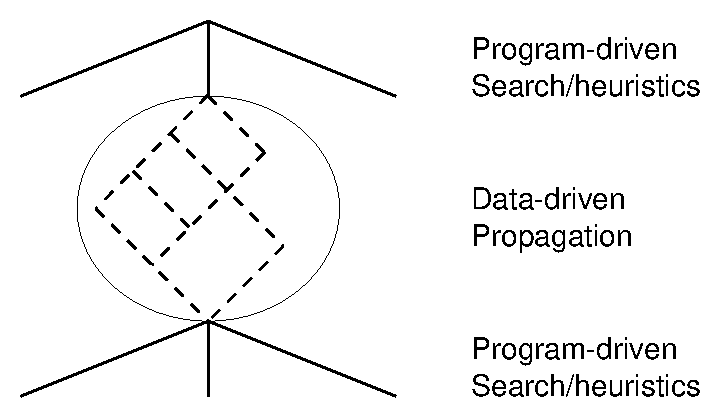
\includegraphics{clpexec.eps}}
\end{center}
\caption{Control during Constraint Solving}
\label{figclpexec}
\end{figure}
Individual constraints can then be implemented with different behaviours,
and freely mixed within a single computation.
Constraint behaviours can essentially be characterised by
\index{trigger condition}
\begin{itemize}
\item their triggering condition ({\bf when} are they executed)
\item the action they perform when triggered ({\bf what} do they do)
\end{itemize}
Let us now look at examples of different constraint behaviours.

\subsection{Consistency Check}
\index{consistency check}
The \verb.=<./2 predicate, whose standard Prolog version raises an error
when invoked with uninstantiated variable, is also implemented by the
{\bf suspend} library. Both implementations
have the same declarative meaning, but the {\bf suspend} version can
be considered to be a proper constraint.
It implements a {\bf passive test}, i.e.\
it simply delays until both arguments are numbers, and then succeeds or fails:
\begin{quote}\begin{verbatim}
?- suspend : (X =< 4).
X = X
There is 1 delayed goal.
Yes (0.00s cpu)

?- suspend : (X =< 4), X = 2.
X = 2
Yes (0.00s cpu)

?- suspend : (X =< 4), X = 5.
No (0.00s cpu)
\end{verbatim}\end{quote}

\subsection{Forward Checking}
\index{forward checking}
Often a constraint can already do useful work before all its arguments
are instantiated. In particular, this is the case when we are working
with domain variables. Consider {\bf ic}'s disequality constraint \verb.#\=.  :
Even when only one side is instantiated, it can already remove this value
from the domain of the other (still uninstantiated) side:
\begin{quote}\begin{verbatim}
?- X :: 1 .. 5,
   X #\= 3.
X = X{[1, 2, 4, 5]}
Yes (0.00s cpu)
\end{verbatim}\end{quote}
If both sides are uninstantiated, the constraint cannot do anything useful.
It therefore waits (delays) until one side becomes instantiated,
but then wakes up and acts as before.
This behaviour is sometimes called forward checking \cite{VanHentenryck}:
\begin{quote}\begin{verbatim}
?- [X,Y] :: 1 .. 5,
   X #\= Y.        % delays
X = X{1 .. 5}
Y = Y{1 .. 5}
There is 1 delayed goal.
Yes (0.00s cpu)

?- X :: 1 .. 5,
   X #\= Y,         % delays
   Y = 3.           % wakes
X = X{[1, 2, 4, 5]}
Y = 3
Yes (0.01s cpu)
\end{verbatim}\end{quote}

\subsection{Domain (Arc) Consistency}
\index{arc consistency}
\index{domain consistency}
For many constraints, even more eager behaviour is possible.
For example, {\bf ic}'s inequality constraints performs {\bf domain updates} as
soon as possible, even when one or both arguments are still variables:
\begin{quote}\begin{verbatim}
?- [X, Y] :: 1 .. 5, X #< Y.
X = X{1 .. 4}
Y = Y{2 .. 5}
There is 1 delayed goal.
Yes (0.00s cpu)

?- [X, Y] :: 1 .. 5, X #< Y, X #> 2.
Y = Y{[4, 5]}
X = X{[3, 4]}
There is 1 delayed goal.
Yes (0.00s cpu)
\end{verbatim}\end{quote}
Inconsistent values are removed form the domains as soon as possible.
This behaviour corresponds to {\bf arc consistency} as discussed in
section \ref{csp}.

\subsection{Bounds Consistency}
\index{bounds consistency}
Note however that not all {\bf ic} constraints maintain full domain
arc consistency.  For performance reasons, 
the \verb.#=. constraint only maintains bounds consistency, which is
weaker, as illustrated by the following example:
\begin{quote}\begin{verbatim}
?- [X, Y] :: 1 .. 5, X #= Y + 1, X #\= 3.
Y = Y{1 .. 4}
X = X{[2, 4, 5]}
There is 1 delayed goal.
Yes (0.00s cpu)
\end{verbatim}\end{quote}
Here, the value 2 for Y was not removed even though it is not arc consistent
(there is no value for X which is compatible with it).

\index{incompleteness of propagation}
It is important to understand that this kind of propagation incompleteness
does not affect correctness: the constraint will simply detect the
inconsistency later, when its arguments have become more instantiated.
In terms of the search tree, this means that a branch will not be pruned
as early as possible, and extra time might be spent searching.


\quickref{Typical Constraint Behaviours}{
\begin{description}
\item[Consistency Checking] 
        wait until all variables instantiated, then check
\item[Forward Checking] 
        wait until one variable left, then compute consequences
\item[Domain (Arc) Consistency] 
        wait until a domain changes, then compute consequences for other domains
\item[Bounds Consistency] 
        wait until a domain bound changes, then compute consequences for other bounds
\end{description}
}


\ignore{
\subsection{The Resolvent}
\index{resolvent}
The term {\bf resolvent} originates from Logic Programming.
It is the set of all goals that need to be satisfied.
The computation typically starts with a top-level goal,
then gets successively transformed (by substituting goals that
match a clause head with an instance of the clause body, ie.\ a
sequence of sub-goals),
and eventually terminates with one of the trivial goals
{\bf true} or {\bf fail}.
For example, given the program
\begin{quote}\begin{verbatim}
p :- q,r.
q.
r :- q.
\end{verbatim}\end{quote}
and the goal p, the resolvent goes through the following states
before the goal is proven and the computation terminates:
\begin{quote}\begin{verbatim}
p ----> q,r ----> r ----> q ----> {}
\end{verbatim}\end{quote}

\index{Prolog}
While in Prolog the resolvent is always processed from left to right,
the resolvent in {\eclipse} is more structured, and can be manipulated
in a much more flexible way.
This is achieved by two basic mechanisms, {\bf suspension}
and {\bf priorities}.

\index{suspended goal}
{\bf Suspended} goals form the part of the resolvent which is
currently not being considered. This is typically done when we
know that we cannot currently infer any interesting information from them.

\index{priority}
The remaining goals are ordered according to their {\bf priority}.
At any time, the system attempts to solve the most urgent subgoal first.
{\eclipse} currently supports a fixed range of 12 different priorities,
priority 1 being the most urgent and 12 the least urgent.

Figure \ref{figresolv} shows the structure of the resolvent.
When a toplevel goal is launched, it has priority 12 and is the only
member of the resolvent. As execution proceeds, active goals may be
suspended, and suspended goals may be woken and scheduled with a
particular priority.
\begin{figure}
% picture has been made with xfig and exported as encapsulated postscript
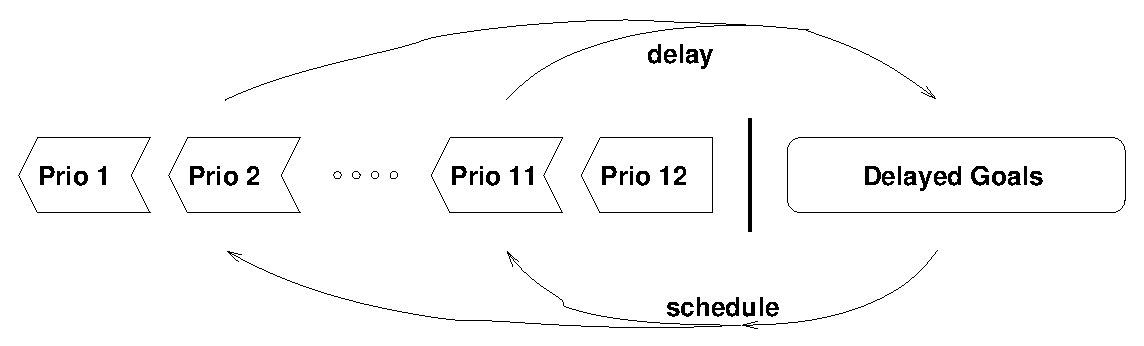
\includegraphics{resolv.eps}
\caption{Structure of the resolvent}
\label{figresolv}
\end{figure}
}



%----------------------------------------------------------------------
\section{Programming Basic Behaviours}
%----------------------------------------------------------------------

As an example, we will look at creating constraint versions of the
following predicate.
It defines a relationship between containers of type 1, 2 or 3,
and their capacity:
\begin{code}
capacity(1, N) :- N>=0.0, N=<350.0.
capacity(2, N) :- N>=0.0, N=<180.0.
capacity(3, N) :- N>=0.0, N=<50.0.
\end{code}
This definition gives the intended declarative meaning,
but does not behave as a constraint:
{\tt capacity(3, C)} will raise an error, and
{\tt capacity(Type, 30.5)} will generate several solutions nondeterministically.
Only calls like {\tt capacity(3, 27.1)} will act correctly as a test.


\subsection{Consistency Check}
\index{consistency check}

To program the passive consistency check behaviour, we need to wait until
both arguments of the predicate are instantiated.
This can be achieved by adding an \eclipse{} {\bf delay clause}:
\begin{code}
delay capacity(T,N) if var(T);var(N).
capacity(1, N) :- N>=0.0, N=<350.0.
capacity(2, N) :- N>=0.0, N=<180.0.
capacity(3, N) :- N>=0.0, N=<50.0.
\end{code}
The delay clause specifies that any call to capacity/2 will delay as long
as one of the arguments is a variable. When the variables become instantiated
later, execution will be resumed automatically, and 
the instantiations will be checked for satisfying the constraint.


\subsection{Forward Checking}
\index{forward checking}

For Forward Checking, we will assume that we have interval domain variables,
as provided by the {\bf ic} library (without domain variables, there would
not be much interesting propagation to be done).

Here is one implementation of a forward checking version:
\begin{code}
:- lib(ic).
delay capacity(T, N) if var(T), var(N).
capacity(T, N) :- nonvar(N), !,
        N >= 0,
        ( N =< 50.0 -> T :: [1,2,3]
        ; N =< 180.0 -> T :: [1,2]
        ; N =< 350.0 -> T = 1
        ; fail
        ).
capacity(1, N) :- N\$>=0.0, N\$=<350.0.
capacity(2, N) :- N\$>=0.0, N\$=<180.0.
capacity(3, N) :- N\$>=0.0, N\$=<50.0.
\end{code}
Note that the delay clause now only lets goals delay when both
arguments are variables. As soon as one is instantiated, the
goal wakes up and, depending on which is the instantiated argument,
either the first, or one of the last three clauses is executed.
Some examples of the behaviour:
\begin{quote}\begin{verbatim}
?- capacity(T, C).
There is 1 delayed goal.
Yes (0.00s cpu)

?- capacity(3, C).
C = C{0.0 .. 50.0}
Yes (0.00s cpu)

?- capacity(T, C), C = 100.
T = T{[1, 2]}
C = 100
Yes (0.00s cpu)
\end{verbatim}\end{quote}

A disadvantage of the above implementation is that when the predicate wakes
up, it can be either because T was instantiated, or because C was
instantiated. An extra check ({\tt nonvar(N)}) is needed to distinguish the two cases.
Alternatively, we could have created two agents (delayed goals), each one
specialised for one of these cases:
\begin{code}
capacity(T, N) :-
        capacity_forward(T, N),
        capacity_backward(T, N).

delay capacity_forward(T, _N) if var(T).
capacity_forward(1, N) :- N\$>=0.0, N\$=<350.0.
capacity_forward(2, N) :- N\$>=0.0, N\$=<180.0.
capacity_forward(3, N) :- N\$>=0.0, N\$=<50.0.

delay capacity_backward(_T, N) if var(N).
capacity_backward(T, N) :-
        N >= 0,
        ( N =< 50.0 -> T :: [1,2,3]
        ; N =< 180.0 -> T :: [1,2]
        ; N =< 350.0 -> T = 1
        ; fail
        ).
\end{code}
Unfortunately, there is a drawback to this implementation as well:
once one of the two delayed goals has done its work, all the constraint's
information has been incorporated into the remaining variable's domain.
However, the other delayed goal is still waiting, and will eventually
wake up when the remaining variable gets instantiated as well, at which time
it will then do a redundant check.

The choice between having one or several agents for a constraint is a
choice we will face every time we implement a constraint.



%----------------------------------------------------------------------
\section{Basic Suspension Facility}
%----------------------------------------------------------------------

For the more complex constraint behaviours (beyond those waiting for
instantiations), we need to employ lower-level primitives of the \eclipse{}
kernel (suspensions and priorities).
\index{suspension}
\index{priority}
If we want to add a new constraint to an existing solver, we also
need to use the lower-level interface that the particular solver
provides.

Apart from the delay clauses used above,
\eclipse{} also provides a more powerful (though less declarative) way of
causing a goal to delay.
The following is another implementation of the constraint checking behaviour,
this time using the suspend/3 built-in predicate to create a delayed goal for
\index{suspend/3}
capacity/2:
\begin{code}
capacity(T,N) :- (var(T);var(N)), !,
        suspend(capacity(T,N), 0, [T,N]->inst).
capacity(1, N) :- N>=0.0, N=<350.0.
capacity(2, N) :- N>=0.0, N=<180.0.
capacity(3, N) :- N>=0.0, N=<50.0.
\end{code}
\quickref{The Basic Suspension Facilities}{
\begin{description}
\item[{\bf suspend(Goal, Priority, Triggers)}] 
	\index{suspend/3}
        Creates Goal as a delayed goal with a given waking priority and
        triggering conditions.
        Triggers is a list of Variables->Conditions terms, specifying
        under which conditions the goal will be woken up.
        The priority specifies with which priority the goal will be scheduled
        after it has been triggered.
        A priority of 0 selects the default for the predicate.
        Otherwise, valid priorities range are from
        1 (most urgent, reserved for debugging purposes) to 12 (least urgent).
\end{description}
Some valid triggers:
\index{trigger condition}
\begin{description}
\item[X->inst] wake when the variable becomes instantiated (most specific)
\item[X->constrained] wake when the variable becomes constrained somehow
        (most general)
\item[X->ic:min] wake when the lower bound of an ic-variable changes
\item[X->ic:max] wake when the upper bound of an ic-variable changes
\item[X->ic:hole] wake an internal domain value gets removed
\end{description}
}


\section{A Bounds-Consistent IC constraint}

To show the basic ideas, we will simply reimplement a constraint that
already exists in the {\bf ic} solver, the inequality constraint.
We want a constraint ge/2 that takes two {\bf ic} variables (or numbers)
and constrains the first to be greater or equal to the second.

\index{bounds consistency}
The behaviour should be to maintain bounds-consistency:
If we have a goal {\tt ge(X,Y)}, where the domain of \verb/X is X{1..5}/ and
the domain of \verb/Y is Y{3..7}/, we would like the domains to be updated such
that the upper bound of Y gets reduced to 5, and the lower bound of X
gets increased to 3. The following code achieves this:
\begin{code}
ge(X, Y) :-
        get_bounds(X, _, XH),
        get_bounds(Y, YL, _),
        ( var(X),var(Y) ->
            suspend(ge(X,Y), 0, [X->ic:max, Y->ic:min])
        ;
            true
        ),
        X #>= YL,    % impose new bounds
        Y #=< XH.
\end{code}
We have used a single primitive from the low-level interface of the
{\bf ic} library:  {\bf get_bounds/3}, which extracts the current
domain bounds from a variable.  Further, we have used the information
that the library implements trigger conditions called {\bf min}
and {\bf max}, which cause a goal to wake up when the lower/upper
bound on an {\bf ic} variable changes.

Note that we suspend a new instance of the {\tt ge(X,Y)} goal {\em before}
we impose the new bounds on the variables. This is important when the
constraint is to be used together with other constraints of higher
priority: imposing a bound may immediately wake and execute such
a higher-priority constraint. The higher-priority constraint may then
in turn change one of the bounds that ought to wake ge/2 again.
This only works if ge/2 has already been (re-)suspended at that time.


\section{Using a Demon}
\index{demon}
Every time the relevant variable bounds change, the delayed ge/2 goal
wakes up and (as long as there are still two variables) a new,
identical goal gets delayed.
To better support this situation, {\eclipse} provides a special type
of predicate, called a {\bf demon}.
A predicate is turned into a
\index{demon}
demon by annotating it with a
\bipref{demon/1}{../bips/kernel/compiler/demon-1.html}
declaration.
A demon goal differs from a normal goal only in its behaviour on
waking. While a normal goal disappears from the resolvent when it is
woken, the demon remains in the resolvent.
Declaratively, this corresponds to an implicit recursive call in
the body of each demon clause.
Or, in other words, the demon goal forks into one goal that remains in the
suspended part of the resolvent, and an identical one
that gets scheduled for execution.

With a demon, our above example can be done more
efficiently. One complication arises, however. Since the goal
implicitly re-suspends, it now has to be explicitly killed when
it is no longer needed. The easiest way to achieve this is to
let it have a handle to itself (its `suspension') in one of its arguments.
This can then be used to kill the suspension when required:
\begin{code}
ge(X, Y) :-
        suspend(ge(X,Y,MySusp), 0, [X->ic:max, Y->ic:min], MySusp),
        ge(X, Y, MySusp).

:- demon ge/3.
ge(X, Y, MySusp) :-
        get_bounds(X, _, XH),
        get_bounds(Y, YL, _),
        ( var(X),var(Y) ->
            true     % implicitly re-suspend
        ;
            kill_suspension(MySusp)
        ),
        X #>= YL,    % impose new bounds
        Y #=< XH.
\end{code}
We have used the new primitives suspend/4 and kill_suspension/1.


%----------------------------------------------------------------------
%\section{Constraints with many variables}
%----------------------------------------------------------------------

%----------------------------------------------------------------------
\section{Exercises}
%----------------------------------------------------------------------

\begin{enumerate}

\item Implement a constraint atmost/3 
\begin{quote}\begin{verbatim}
atmost(+N, +List, +V)
\end{verbatim}\end{quote}
   which takes an integer N, an integer V and a list List
   containing integers or integer domain variables.

   Meaning: at most N elements of List have value V.

   Behaviour: Fail as soon as too many list elements are
   instantiated to value V.
   This requires only basic suspension facilities, no domain
   information needs to be taken into account.

   Tests are provided in the file {\tt atmost.tst}.
   You can test your constraint by loading the library {\tt lib(test_util)}
   and then calling {\tt test(atmost)}.


\item Implement a constraint offset/3

\begin{quote}\begin{verbatim}
offset(?X,+Const,?Y)
\end{verbatim}\end{quote}
which is declaratively like
\begin{quote}\begin{verbatim}
offset(X,Const,Y) :- Y #= X+Const.
\end{verbatim}\end{quote}
  but maintains domain-arc-consistency (i.e. propagates
  "holes", while the above definition only maintains
  bounds-consistency).

  Use suspension built-ins and domain-access primitives
  from the ic_kernel module.
  Use not_unify/2 to test whether a value is outside
  a variable's domain.

   Tests are provided in the file {\tt offset.tst}.
   You can test your constraint by loading the library {\tt lib(test_util)}.
   and then calling {\tt test(offset)}.

\end{enumerate}

%HEVEA\cutend

% BEGIN LICENSE BLOCK
% Version: CMPL 1.1
%
% The contents of this file are subject to the Cisco-style Mozilla Public
% License Version 1.1 (the "License"); you may not use this file except
% in compliance with the License.  You may obtain a copy of the License
% at www.eclipse-clp.org/license.
% 
% Software distributed under the License is distributed on an "AS IS"
% basis, WITHOUT WARRANTY OF ANY KIND, either express or implied.  See
% the License for the specific language governing rights and limitations
% under the License. 
% 
% The Original Code is  The ECLiPSe Constraint Logic Programming System. 
% The Initial Developer of the Original Code is  Cisco Systems, Inc. 
% Portions created by the Initial Developer are
% Copyright (C) 2006 Cisco Systems, Inc.  All Rights Reserved.
% 
% Contributor(s): 
% 
% END LICENSE BLOCK

\chapter{Propia and CHR}
\label{chappropiachr}
%HEVEA\cutdef[1]{section}

\section{Two Ways of Specifying Constraint Behaviours}
There are two elegant and simple ways of building constraints
available in \eclipse{}, called {\em Propia} and {\em Constraint
Handling Rules} (or {\em CHR}'s).  
They are themselves built using the facilities
described in chapter \ref{chapimpl}.

\index{noclash}
Consider a simple {\em noclash} constraint requiring that two
activities cannot be in progress at the same time.  
For the sake of the example, the constraint involves two variables,
the start times $S1$ and $S2$ 
of the two activities, which both have duration $5$.
Logically this constraint states that
{\em noclash} $ \Leftrightarrow (S1 >= S2 + 5 \vee S2 >= S1 + 5)$.
The same logic can be expressed as two \eclipse{} clauses:
\begin{code}
noclash(S1,S2) :-
    ic:(S1 \$>= S2+5).
noclash(S1,S2) :-
    ic:(S2 \$>= S1+5).
\end{code}
Constraint propagation elicits information from constraints without
leaving any choice points.  Constraint propagation behaviour can be
associated with each of the above representations, by CHR's
and by Propia.

One way to propagate information from {\em noclash} is to wait until
the domains of the start times are reduced sufficiently that only one
ordering of the tasks is possible, and then to enforce the constraint
that the second task not start until the first is finished.

\index{constraints/1}
This behaviour can be implemented in CHR's as follows:
\begin{code}
:- constraints noclash/2.
noclash(S1,S2) <=> ic:(S2 #< S1+5) | ic:(S1 #>= S2+5).
noclash(S1,S2) <=> ic:(S1 #< S2+5) | ic:(S2 #>= S1+5).
\end{code}

Consider the query:
\begin{quote}
\begin{verbatim}
?- ic:([S1,S2]::1..10),
   noclash(S1,S2),
   S1 #>= 6.
\end{verbatim}
\end{quote}
In this query {\em noclash} achieves no propagation when it is
initially posted with the start time domains set to \verb91..109.
However, after imposing $S1>=6$, 
the domain of $S1$ is reduced to \verb96..109.
Immediately the {\em noclash}
constraint wakes, detects that the first
condition $S1+5 >= S2$ is entailed, 
and narrows the domain of $S2$ to \verb91..59.

The same behaviour can be expressed in Propia, but this time the
original \eclipse{} representation of {\em noclash} as two clauses is
used directly.  The propagation behaviour is automatically
extracted from the two clauses by Propia when the {\em noclash} goal
is annotated as follows:
\begin{quote}
\begin{verbatim}
?-      [S1,S2]::1..10,
        noclash(S1,S2) infers most,
        S1 #>= 6.
\end{verbatim}
\end{quote}
%For readability \verb0infers0 is declared to be an infix operator,
%enabling the annotation to be written thus: 
%\begin{quote}
%\begin{verbatim}
%?- [S1,S2]::1..10, noclash(S1,S2) infers most, S1 #>= 6
%\end{verbatim}
%\end{quote}

\quickref{Building Constraints without Tears}{
Propia and CHRs make it easy to turn the logical statement of a
constraint into code that efficiently enforces that constraint.
}

\section{The Role of Propia and CHR in Problem Modelling}

\index{modelling}
To formulate and solve a problem in \eclipse{} the standard pattern is
as follows:
\begin{enumerate}
\item Initialise the problem variables
\item State the constraints
\item Specify the search behaviour
\end{enumerate}
Very often, however, the constraints involve logical implications or
disjunctions, as in the case of the {\em noclash} constraint above.   
Such constraints are most naturally formulated in a way that would
introduce choice points during the constraint posting phase. 
The two \eclipse{} clauses defining {\em noclash}, above, are a case in
point. 

There are two major disadvantages of introducing choice points during
constraint posting:
\begin{itemize}
\item Posting and reposting constraints during search is an
unnecessary and computationally expensive overhead
\item Mixing constraint behaviour and search behaviour makes it harder
to explore and optimize the algorithm executed by the program.
\end{itemize}
Propia and CHR's support the separation of constraint setup and search
behaviour, by allowing constraints to be formulated naturally without
their execution setting up any choice points.

The effect on performance is illustrated by the following small
example.
The aim is to choose a set of $9$ products (\verb0Products0,
identified by their product number 101-109) to
manufacture, with a 
limited quantity of raw materials (\verb0Raw10 and \verb0Raw20), 
so as to achieve a profit (\verb0Profit0) of over
$40$.  
The amount of raw materials (of two kinds) needed to produce
each product is listed in a table, together with its profit.

\index{product\_plan}
\index{product}
\begin{code}
product_plan(Products) :-
    length(Products,9),
    Raw1 #=< 95,
    Raw2 #=< 95,
    Profit #>= 40,
    sum(Products,Raw1,Raw2,Profit),
    labeling(Products).

product( 101,1,19,1).  product( 102,2,17,2).  product( 103,3,15,3).
product( 104,4,13,4).  product( 105,10,8,5).  product( 106,16,4,4).
product( 107,17,3,3).  product( 108,18,2,2).  product( 109,19,1,1).

sum(Products,Raw1,Raw2,Profit) :-
    ( foreach(Item,Products),
      foreach(R1,R1List),
      foreach(R2,R2List),
      foreach(P,PList)
    do
        product(Item,R1,R2,P)
    ),
    Raw1 #= sum(R1List),
    Raw2 #= sum(R2List),
    Profit #= sum(PList).

\end{code}

The drawback of this program is that the \verb0sum0 constraint calls
\verb0product0 which chooses an item and leaves a choice point at each
call. 
Thus the setup of the \verb0sum0 constraint leaves $9$ choice points.
Try running it, and the program
fails to terminate within a reasonable amount of time.

Now to make the program run efficiently, we can simply annotate the call
to \verb0product0 as a Propia constraint making:
\verb0product(Item,R1,R2,P) infers most0.
This program leaves no choice points during constraint setup, and
finds a solution in a fraction of a second.

In the remainder of this chapter we show how to use Propia and CHR's,
give some 
examples, and outline their implementation.

\quickref{Modelling without Choice Points}{
Propia and CHRs can be used to build clear problem models that have no
(hidden) choice points.
}

\section{Propia}
\label{secpropia}

\index{propia}
\index{generalised propagation}
Propia is an implementation of {\em Generalised Propagation}
which is described in the paper  \cite{LeProvost93b}.

\subsection{How to Use Propia}
\index{infers/2}
In principle Propia propagates information from an annotated goal by
finding all solutions to the goal and extracting any information that
is common to all the different solutions.
(In practice, as we shall see later, Propia does not typically need to
find all the solutions.)

The ``common'' information that can be extracted depends upon what
constraint solvers are used when evaluating the underlying
un-annotated \eclipse{} goal.  To illustrate this, consider another
simple example.

\begin{quote}
\begin{verbatim}
p(1,3).
p(1,4).

?-  p(X,Y) infers most.
\end{verbatim}
\end{quote}
If the {\tt ic} library is not loaded when this query is
invoked, then the information propagated by Propia is that $X=1$.
If, on the other hand, {\tt ic} is loaded, then more common
information is propagated.  Not only does Propia propagate $X=1$ but
also the domain of $Y$ is tightened from \verb0-inf..inf0 to 
\verb03..40. (In this case the additional common information is that
$Y \neq  0$, $Y \neq 1$, $Y \neq 2$ and so on for all values except $3$
and $4$!)

\index{most}
\index{consistent}
\index{unique}
\index{ac}
Any goal \verb0Goal0 in an \eclipse{} program, can be transformed into a
constraint by annotating it thus: \verb0Goal infers Parameter0.
Different behaviours can be specified with different parameters, viz:
\begin{itemize}
\item \verb0Goal infers most0\\
Propagates all common information produced by the loaded solvers
\item \verb0Goal infers unique0\\
Fails if there is no solution, propagates the solution if it is
unique, and succeeds without propagating further information if there
is more than one solution.
\item \verb0Goal infers consistent0\\
Fails if there is no solution, and propagates no information otherwise 
\end{itemize}

%\item \verb0Goal infers ic0\\
%Tightens the domains of the variables.  
%\item \verb0Goal infers ac0\\
%Tightens the domains of the variables: more efficient than \verb0ic0,
%but can only handle goals with a finite set of ground answers.

\index{crossword}
These behaviours are nicely illustrated by the crossword demonstration
program \verb0crossword0 in the examples code directory.
There are 72 ways to complete the crossword grid with words from the
accompanying directory.  
For finding all 72 solutions,
the comparative performance of the different annotations is given in the
table {\em Comparing Annotations}.

\begin{table}[tb]
\begin{center}
\begin{tabular}{|c|c|c|c|}
\hline
Annotation & CPU time (secs)\\
\hline
consistent & 13.3 \\
unique & 2.5 \\
most & 9.8 \\
ac & 0.3 \\
\hline
\end{tabular}
\end{center}
\caption{Comparing Annotations}
\end{table}

The example program also illustrates the effect of specifying the waking
conditions for Propia.  By only waking a Propia constraint when it
becomes instantiated, the time to solve the crossword problem can be
changed considerably.  For example by changing the annotation from
\verb0Goal infers most0 to 
\verb0suspend(Goal,4,Goal->inst) infers most0 
the time needed to find all solutions goes down from 10 seconds to
just one second.

For other problems, such as the square tiling problem in the example
directory, the fastest version is the 
one using \verb0infers consistent0.  To find the best Propia
annotation it is necessary to experiment with the current problem
using realistic data sets.

\quickref{Transforming Procedures to Constraints}{
Propia extracts information from a procedure which may be defined by
multiple \eclipse{} clauses.  
The information to be extracted is
controlled by the Propia annotation.
% (e.g. \verb0consistent0, \verb0unique0, \verb0most0 and \verb0ac0).
}

\subsection{Propia Implementation}
In this section we describe how Propia works.

\subsubsection{Outline}
When a goal is annotated as a Propia constraint, eg. 
\verb0p(X,Y) infers most0, first the goal \verb0p(X,Y)0 is in effect 
evaluated in the normal way by \eclipse{}.
However Propia does not stop at the first solution, but continues to
find more and more solutions, each time combining the information from
the solutions retrieved.
When all the information has been accumulated, Propia propagates this
information (either by narrowing the domains of variables in the goal,
or partially instantiating them).

Propia then suspends the goal again, until the variables become
further constrained, at which point it wakes, extracts information
from solutions to the more constrained goal, propagates it, and
suspends again.

If Propia detects that the goal is entailed (i.e. the goal would
succeed whichever way the variables were instantiated), then after
propagation it does not suspend any more.

\subsubsection{Most Specific Generalisation}
\index{most specific generalisation}
\index{MSG}
Propia works by treating its input both as a {\em goal} to be called,
and as a term which can be manipulated as data.
As with any \eclipse{} goal, when executed its result is a further
instantiation of the term.  
For example the first result of calling \verb0member(X,[a,b,c])0 is
to further instantiate the term yielding \verb0member(a,[a,b,c])0.
This instantiated term represents the (first) solution to the goal.

Propia combines information from the solutions to a goal using their
{\em most specific generalisation} ({\em MSG}).
The MSG of two terms is a term
that can be instantiated (in different ways) to either of the two
terms. For example
$p(a,f(Y))$ is the MSG of $p(a,f(b))$ and $p(a,f(c))$.
This is the meaning of {\em generalisation}. 
The meaning of {\em most specific} is that any other term that
generalises the two terms, is more general than the MSG.
For example, any other term that generalises $p(a,f(b)$ and
$p(a,f(c))$ can be instantiated to $p(a,f(Y))$.
The MSG of two terms captures only information that is common to both
terms (because it generalises the two terms), and it captures all the
information possible in the two terms (because it is the most specific
generalisation).

Some surprising information is caught by the MSG.  For example the MSG
of $p(0,0)$ and $p(1,1)$ is $p(X,X)$.
We can illustrate this being exploited by Propia in the following
example:
\begin{code}
% Definition of logical conjunction
conj(1,1,1).
conj(1,0,0).
conj(0,1,0).
conj(0,0,0).

conjtest(X,Z) :-
    conj(X,Y,Z) infers most,
    X=Y.
\end{code}
The test succeeds, recognising that $X$ must take the same truth value
as $Z$.  Running this in \eclipse{} yields:
\begin{quote}
\begin{verbatim}
[eclipse]: conjtest(X,Z).
X = X
Z = X
Delayed goals:
        conj(X, X, X) infers most
Yes (0.00s cpu)
\end{verbatim}
\end{quote}

If the {\tt ic} library is loaded more information can be extracted,
because the MSG of $0$ and $1$ is a variable with domain \verb90..19.
Thus the result of the above example is not only to equate $X$ and $Z$
but to associate with them the domain \verb90..19.

The MSG of two terms depends upon what information is expressible in
the MSG term.  As the above example shows, if the term can employ
variable domains the MSG is more precise. 

By choosing the class of terms in which the MSG can be
expressed, we can capture more or less information in the MSG.
If, for example, we allow only terms of maximum depth 1 in the class,
then MSG can only capture functor and arity.
In this case the MSG of $f(a,1)$ and $f(a,2)$ is simply $f(_,_)$, even
though there is more shared information at the next depth.

In fact the class of terms can be extended to a lattice, by
introducing a bottom $\bot$ and a top $\top$.  
$\bot$ is a term carrying no
information; $\top$ is a term representing inconsistent information;
the 
meet of two terms is the result of unifying them; and their join is
their MSG.

\subsubsection{The Propia Algorithm}
We can now specify the Propia algorithm more precisely.
The Propia constraint is 
\begin{verbatim}Goal infers Parameter \end{verbatim}

\begin{itemize}
\item  Set $OutTerm := \top$
\item  Repeat
\begin{itemize}
\item   Find a solution $S$ to $Goal$ which is {\em not} an instance of
$OutTerm$  
\item   Find the MSG, in the class specified by \verb0Parameter0, 
of $OutTerm$ and $S$.  Call it $MSG$
\item   Set $OutTerm := MSG$
\end{itemize}
until either $Goal$ is an instance of $OutTerm$, or no such
solution remains 
\item Return $OutTerm$
\end{itemize}

When \verb0infers most0 is being handled, the class of terms admitted
for the MSG is the biggest class expressible in terms of the currently
loaded solvers.  In case $ic$ is loaded, this includes variable
domain, but otherwise it includes any \eclipse{} term without variable
attributes.

The algorithm supports \verb0infers consistent0 by admitting only the
two terms $\top$ and $\bot$ in the MSG class.
\verb0infers unique0 is a variation of the algorithm in which the
first step $OutTerm := \top$ is changed to finding a first solution
$S$ to $Goal$ and initialising $OutTerm := S$.

Propia's termination is dramatically improved by the check that the
next solution found is not an 
instance of $OutTerm$.  In the absence of domains, there is no
infinite sequence of terms that strictly generalise each other.
Moreover, if
the variables in $Goal$ have finite domains, the same result holds. 
Thus, because of this check, Propia will terminate as long as each
call of $Goal$ terminates. 

For example the Propia constraint 
\verb0member(Var,List) infers Parameter0 will 
always terminate, if each call of \verb0member(Var,List)0 does, even in
case 
\verb0member(Var,List)0 has infinitely many solutions!

\quickref{Most Specific Generalisation}{
Propia computes the Most Specific Generalisation (MSG) of the set of
solutions to a procedure.  It does so without, necessarily,
backtracking through all the solutions to the procedure.
The MSG depends upon the annotation of the Propia call.
}

\subsection{Propia and Related Techniques}
If the finite domain solver is loaded then \verb0Goal infers most0 prunes
the variable domains so every value is supported by values in the
domains of the other variables.  If every problem constraint was
annotated this way, then Propia would enforce arc consistency.

\index{arc consistency}
Propia generalises traditional arc consistency in two ways.  Firstly
it admits n-ary constraints, and secondly it handles predicates
defined by rules, as well as ground facts.  In the special case that
the goal can be ``unfolded'' into a finite set of ground solutions,
this can be exploited by using \verb0infers ac0 to make Propia run
more efficiently.   When called with parameter \verb0infers ac0,
Propia simply finds all solutions and 
applies n-ary arc-consistency to the resulting tables.

%associates an identifier with each tuple.  Arc-consistency is then
%applied to the binary constraints between the tuple identifiers and
%tuple values for each attribute, using the \verb0element0 constraint
%in the {\tt ic} library.

\index{constructive disjunction}
Propia also generalises {\em constructive disjunction}.  Constructive
disjunction could be applied in case the
predicate was unfolded into a finite set of solutions, where each
solution was expressed using {\tt ic} constraints (such as equations,
inequations etc.).
Propia can also handle recursively defined predicates, like
\verb0member0, exampled above, which may have an infinite number of
solutions. 


\section{CHR}
\label{secchr}
\index{CHR}
Constraint Handling Rules were originally implemented in \eclipse{}.
They are introduced in the paper \cite{Fruehwirth}.

\subsection{How to Use CHR}
\index{simplification rule}
\index{propagation rule}
CHR's offer a rule-based programming style to express constraint
simplification and constraint propagation.
The rules all have a {\em head}, an explicit or implicit {\em guard},
and a {\em body}, and are written either
\begin{quote}
\begin{verbatim}
Head <=> Guard | Body.  %Simplification Rule
\end{verbatim}
\end{quote}
or
\begin{quote}
\begin{verbatim}
Head ==> Guard | Body.   %Propagation Rule
\end{verbatim}
\end{quote}
When a constraint is posted that is an instance of the head, the guard
is checked to determine whether the rule can fire.
If the guard is satisfied (i.e. CHR detects that it is entailed by the
current search state), the 
rule {\em fires}. 
Unlike \eclipse{} clauses, the rules leave no choice points.
Thus if several rules share the same head and one fires, the other
rules are never fired even after a failure.

Normally the guards exclude each other, as in the \verb0noclash0
example:
\begin{code}
:- lib(ech).
:- constraints noclash/2.
noclash(S1,S2) <=> ic:(S2 #< S1+5) | ic:(S1 #>= S2+5).
noclash(S1,S2) <=> ic:(S1 #< S2+5) | ic:(S2 #>= S1+5).
\end{code}
Henceforth we will not explicitly load the {\tt ech} library.

The power of guards lies in the behaviour of the rules when they are
neither entailed, nor disentailed.
Thus in the query
\begin{quote}
\begin{verbatim}
?- ic:([S1,S2]::1..10),
   noclash(S1,S2),
   S1 #>= 6.
\end{verbatim}
\end{quote}
\begin{sloppypar}
when the \verb0noclash0 constraint is initially posted, neither guard
is entailed, and CHR simply postpones the handling of the constraint
until further constraints are posted.
As soon as a guard becomes entailed, however, the rule fires.
For simplification rules, of the form 
\verb0Head <=> Guard | Body0, 
the head is replaced by the body.
In this example, therefore, \verb0noclash(S1,S2)0 is replaced by
\verb0S1 #>= S2+50.
\end{sloppypar}

Propagation rules are useful to add constraints, instead of replacing
them.
Consider, for example, an application to temporal reasoning.
If the time $T1$ is before time $T2$, then we can propagate an
additional $ic$ constraint saying $T1 =< T2$:
\begin{code}
:- constraints before/2.
before(T1,T2) ==> ic:(T1 \$=< T2)
\end{code}
This rule simply posts the constraint \verb0T1 $=< T20 to $ic$.
When a propagation rule fires its body is invoked, but its head
remains in the constraint store.

\subsection{Multiple Heads}

Sometimes different constraints interact, and more can be deduced
from the combination of constraints than can be deduced from the
constraints separately.  Consider the following query:
\begin{quote}
\begin{verbatim}
?- ic:([S1,S2]::1..10),
   noclash(S1,S2),
   before(S1,S2).
\end{verbatim}
\end{quote}
Unfortunately the {\tt ic} bounds are not tight enough for the
\verb0noclash0 rule to fire.
The two constraints can be combined so as to propagate $S2 \ge S1+5$
using a two-headed
CHR:
\begin{quote}
\begin{verbatim}
noclash(S1,S2), before(S1,S2) ==> ic:(S2 #>= S1+5).
\end{verbatim}
\end{quote}
We would prefer to write a set of rules that captured this kind of
inference in a general way.

\index{simpagation rule}
This can be achieved by writing a more complete solver for
\verb0prec0, and combining it with \verb0noclash0.
$prec(S1,D,S2)$ holds if the time $S1$ precedes the time $S2$ by at
least $D$ units of time.
For the following code to work, $S1$ and $S2$ may be numbers or
variables, but $D$ must be a number.
\begin{code}
:- constraints prec/3.
prec(S,D,S) <=> D=<0.
prec(S1,0,S2), prec(S2,0,S1) <=> S1=S2.
prec(S1,D1,S2), prec(S2,D2,S3) ==> D3 is D1+D2, prec(S1,D3,S3).
prec(S1,D1,S2) \verb.\. prec(S1,D2,S2) <=> D2=<D1 | true.     % Simpagation

noclash(S1,S2), prec(S1,D,S2) ==> D > -5 | prec(S1,5,S2).
noclash(S1,S2), prec(S2,D,S1) ==> D > -5 | prec(S2,5,S1).
\end{code}
Note the {\em simpagation} rule, whose head has two parts 
\verb0Head1 \ Head20. 
In a simpagation rule \verb0Head20 is replaced, but \verb0Head10 is
kept in the constraint store.

\quickref{CHRs}{
CHRs are guarded rules which fire without leaving choice points.
A CHR rule may have one or many goals in the head, and may take the
following forms: Simplification rule, Propagation rule or Simpagation
rule. 
%\begin{itemize}
%\item[{\em Simplification} rule] \verb0Head <=> Guard | Body0
%\item[{\em Propagation} rule] \verb0Head ==> Guard | Body0
%\item[{\em Simpagation} rule] \verb0Head1 \ Head2 <=> Guard | Body0
%\end{itemize}

}

\section{A Complete Example of a CHR File}

Sometimes whole sets of constraints can be combined.
Consider, for example, a program where disequalities on pairs of
variables are accumulated during search.
Whenever a point is reached where any subset of the variables are all
constrained to be different an \verb0alldifferent0 constraint can be
posted on that subset, thus supporting more powerful propagation.
This can be achieved by finding {\em cliques} in the graph whose nodes
are variables and edges are disequality constraints.

\index{clique}
We start our code with a declaration to load the {\em ech} library.
The constraints are then declared, and subsequently defined by rules.
The CHR encoding starts by generating a clique whenever two variables
are constrained to be different.
\begin{code}
:- lib(ech).
:- constraints neq/2.

neq(X,Y) ==>
    sort([X,Y],List),
    clique(List),
    neq(Y,X).
\end{code}
Each clique is held as a sorted list to avoid any duplication.
The symmetrical disequality is added to simplify the detection of new
cliques, below.
Whenever a clique is found, the \verb0alldifferent0 constraint is
posted, and the CHRs seek to extend this clique to
include another variable:
\begin{code}
:- constraints clique/1.

clique(List) ==> alldifferent(List).
clique(List),neq(X,Y) ==>
    in_clique(Y,List), not in_clique(X,List) |
    sort([X|List],Clique),
    extend_clique(X,List,Clique).

in_clique(Var,List) :-
    member(El,List), El==Var, !.
\end{code}
The idea is to search the constraint store for a disequality between
the new variable \verb0X0 and each other variable in the original
clique.  This is done by recursing down the list of remaining
variables.
When there are no more variables left, a new clique has been found.
\begin{code}
neq(X,Y) \verb.\. extend_clique(X,[Y|Tail],Clique) <=>
    extend_clique(X,Tail,Clique).
extend_clique(_,[],Clique) <=> 
    clique(Clique).
\end{code}

Finally, we add three optimisations.
Don't try and find a clique that has already been found, or
find the same clique twice.  If the new variable is equal to a
variable in the list, then don't try any further.
\begin{code}
clique(Clique) \verb.\. extend_clique(_,_,Clique) <=> true.
extend_clique(_,_,Clique) \verb.\. extend_clique(_,_,Clique) <=> true.
extend_clique(Var,List,_) <=> in_clique(Var,List) | true.
\end{code}

\subsection{CHR Implementation}
CHR's are implemented using the \eclipse{} suspension and waking
mechanisms. 
A rule is woken if:
\begin{itemize}
\item a new goal is posted, which matches one of the goals in its head
\item a goal which has already been posted earlier becomes further
instantiated.
\end{itemize}

\index{entailment}
The rule cannot fire unless the goal is more instantiated than the
rule head.  Thus the rule
\verb0p(a,f(Y),Y) <=> q(Y)0 is really a shorthand for the guarded
rule:
\begin{quote}
\begin{verbatim}
p(A,B,C) <=> A=a, B=f(Y), C=Y | q(Y)
\end{verbatim}
\end{quote}
The guard is ``satisfied'' if, logically, it is entailed by the
constraints posted already.

In practice the CHR implementation cannot always detect the
entailment.
The consequence is that goals may fire later than they could.
For example consider the program
\begin{code}
:- constraints p/2.
p(X,Y) <=> ic:(X \$> Y) | q(X,Y).
\end{code}
and the goal
\begin{quote}
\begin{verbatim}
?-  ic:(X $> Y),
    p(X,Y).
\end{verbatim}
\end{quote}
Although the guard is clearly satisfied, the CHR implementation cannot
detect this and \verb0p(X,Y)0 does not fire.
If the programmer needs the entailment of inequalities to be detected,
it is necessary to express inequalities as CHR constraints, which
propagate {\tt ic} constraints as illustrated in the example
\verb0prec(S1,D,S2)0 above.

CHRs can detect entailment via variable bounds, so \verb.p(X,0).
does fire in the following example:
\begin{quote}
\begin{verbatim}
?-  ic:(X $> 1),
    p(X,0).
\end{verbatim}
\end{quote}

The implementation of this entailment test in \eclipse{} is to impose
the guard as a constraint, and fail (the entailment test) as soon as
any variable becomes more constrained.
A variable becomes more constrained if:
\begin{itemize}
\item it becomes more instantiated
\item its domain is tightened
\item a new goal is added to its suspension list
\end{itemize}

There are many examples of applications expressed in CHR in the
\eclipse{} distribution.
They are held as files in the {\em chr} subdirectory of the standard
\eclipse{} library directory {\em lib}. 

\quickref{CHR Implementation}{
CHRs suspend on the variables in the rule head.  On waking the CHR
tests if its guard is entailed by the current constraint store.  The
entailment test is efficient but incomplete, and therefore rules may
fail to fire as early as they could in theory.
}

\section{Global Reasoning}
\index{global reasoning}
Constraints in {\tt ic} are handled separately and individually.  More
global consistency techniques can be achieved using global
constraints.
Propia and CHRs provide alternative methods of achieving more global
consistency.
Propia allows any subproblem to be treated as a single constraint.
CHRs allow any set of constraints to be handled by a single rule.
Each technique has special strengths.  Propia is good for handling
complicated logical combinations of constraints.  CHRs are good for
combining sets of constraints to extract transitive closures, and
cliques.

Both are fun to implement and use!

\section{Propia and CHR Exercise}


The problem is to implement three constraints, \verb'and', \verb'or'
and \verb'xor' 
in CHRs and, as a separate exercise, in Propia.
The constraints are specified as follows:
All boolean variables have domain $\{0,1\}$: $0$ for 'false' and $1$
for 'true'. 
\begin{quotation}
\noindent and(X,Y,Z) =def (X \& Y) = Z\\
or(X,Y,Z)  =def (X or Y) = Z\\
xor(X,Y,Z) =def ((X \& -Y) or (-X \& Y)) = Z
\end{quotation}

Suppose your constraints are called 
\verb0cons_and0, \verb0cons_or0 and \verb0cons_xor0
Now write enter the following procedure:
\begin{code}
full_adder(I1,I2,I3,O1,O2) :-
    cons_xor(I1,I2,X1),
    cons_and(I1,I2,Y1),
    cons_xor(X1,I3,O1),
    cons_and(I3,X1,Y2),
    cons_or(Y1,Y2,O2).
\end{code}
The problem is solved if you enter the query:
\begin{quote}
\begin{verbatim}
?- full_adder(I1,I2,0,O1,1).
\end{verbatim}
\end{quote}
and get the correct answer.

Note: you are not allowed to load the ic library nor to use search and
backtracking!

%HEVEA\cutend

% BEGIN LICENSE BLOCK
% Version: CMPL 1.1
%
% The contents of this file are subject to the Cisco-style Mozilla Public
% License Version 1.1 (the "License"); you may not use this file except
% in compliance with the License.  You may obtain a copy of the License
% at www.eclipse-clp.org/license.
% 
% Software distributed under the License is distributed on an "AS IS"
% basis, WITHOUT WARRANTY OF ANY KIND, either express or implied.  See
% the License for the specific language governing rights and limitations
% under the License. 
% 
% The Original Code is  The ECLiPSe Constraint Logic Programming System. 
% The Initial Developer of the Original Code is  Cisco Systems, Inc. 
% Portions created by the Initial Developer are
% Copyright (C) 2006 Cisco Systems, Inc.  All Rights Reserved.
% 
% Contributor(s): 
% 
% END LICENSE BLOCK

%HEVEA\cutdef[1]{section}

\index{mathematical programming, interface to|(}
\index{mixed integer programming, interface to|(}
\index{linear programming, interface to|(}
\index{quadratic programming, interface to|(}
\index{simplex solver, interface to|(}
\section{Usage}
This library allows the use of an external mathematical programming 
(LP, MIP or quadratic) solver 
from within {\eclipse}. It provides a largely solver-independent API
to the programmer, so many programs will run with any supported external
solver.

The library interfaces to both commercial and open-source
solvers. Commercial solver will probably require a license to use the
solver, while the open-source solvers are available free of charge, but are
govererned by their own open-source licenses separate from {\eclipse}'s.

%With the kind agreement of Dash Associates Ltd., the
%XPRESS-MP\footnote{XPRESS-MP is a product from Dash Associates
%Ltd. (www.dashoptimization.com)} solver is now included with the library,
%and is available for academic use under the {\eclipse} licence agreement.

See section~\ref{specificsolver} for more details on the supported solvers.

The most generic way to load the library is:
\begin{verbatim}
:- lib(eplex).
\end{verbatim}
\index{eplex}
This will try to load an appropriate external solver available on
the computer.

It is also possible to request a specific solver explicitly,
see section~\ref{specificsolver} for details.

Note that the {\eclipse} library described here is just an interface
to an external solver. In order to be able to use it, you need to have
access to a solver supported by the library. For commercial solvers, this
requires a licence for the solver on your machine. For more details,
see section \ref{specificsolver}. For open source solvers, the required
solver library may be distributed with {\eclipse} if its licence allows
this.


%\section{History}
%The latest major addition to this library is support for adding
%constraints to the solver, as far as this is supported by the
%external solver.
%
%The library has been ported to work with XPRESS-MP as well as CPLEX.
%
%The third version of this library uses standard range-variables
%provided by the \htmlref{range-library}{chaprange}, which should
%facilitate interfacing to other solvers.
%The interface to CPLEX has been extended such that more
%state information can be retrieved, e.g.\ constraint slacks,
%basis information, reduced costs etc.
%A quite generic solver demon is provided which makes it easy to
%use CPLEX within a data-driven CLP setting.
%
%The second major version made some things conceptually clearer.
%The notion of solver handles is new. It removes the ugly
%concept of a global state and hopefully encourages
%experiments with multiple solvers.
%The interface to the solver's state has been extended,
%allowing to modify and query many parameters and extract
%solution information.
%A pair of predicates has been added to allow reading and writing
%problem files in MPS or LP format.
%


%----------------------------------------------------------------------
\section{Eplex Instances}
%----------------------------------------------------------------------

In this chapter, the problem passed to the external solver will be referred
to as an {\it eplex problem}. An eplex problem consists of a set of linear
arithmetic constraints, whose variables have bounds and may possibly have
integrality constraints. The external solver will solve such a problem by optimising
these constraints with respect to an objective function. 

With the eplex library, it is possible to have more than one eplex problem
within one program. The simplest way to write such programs with the
library is through {\it Eplex Instances}. An eplex instance is an instance
of the eplex solver, to which an eplex problem can be sent. An external
{\it solver state} can be associated with each eplex instance, which can be
invoked to solve the eplex problem. Declaratively, an eplex instance can be
seen as a compound constraint consisting of all the variables, their bounds, and
constraints of the eplex problem.

Like other solvers, each eplex instance has its own module. To use an eplex
instance, it must first be declared, so that the module can be created.
This is done by:

\subsubsection{\biptxtref{eplex_instance(+Name)}{eplex_instance/1}{../bips/lib/eplex/eplex_instance-1.html}}

This predicate will initialise an eplex instance {\tt Name}. Once
initialised, a {\tt Name} module will exist, to which the user can post the 
constraints for the eplex problem and setup and use the external solver
state to solve the eplex problem. Normally, this predicate should be issued
as a directive in the user's program, so that the program code can refer to
the instance directly in their code. For example:

\begin{verbatim}
   :- eplex_instance(instance).
\end{verbatim}


For convenience, the eplex library declares {\tt eplex} as an eplex instance 
when the library is loaded. 

\subsection{Linear Constraints}
\label{linear-constraints}
The constraints provided are equalities and inequalities over
linear expressions. 
Their operational behaviour is as follows:
\begin{itemize}
\item When they contain no variables, they simply succeed or fail.
\item When they contain exactly one variable, they are translated into
a bound update on that variable, which may in turn fail, succeed,
or even instantiate the variable.
Note that if the variable's type is integer, the bound will be adjusted
to the next suitable integral value.
\item Otherwise, the constraint is transferred to the external solver state
if the state has been setup. If it has not, the constraint
delays and is transferred to the external solver state when it is setup.
This mechanism makes it possible to interface to a non-incremental
black-box solver that requires all constraints at once,
or to send constraints to the solver in batches
\end{itemize}


As with all predicates defined for an eplex instance, these constraints
should be module-qualified with the name of the eplex instance. In the 
following they are shown qualified with the {\tt eplex} instance, and with 
brackets around the constraints when needed. Other instances can
be used if they have been declared using {\bf eplex_instance/1}. 
 
\subsubsection{\biptxtrefni{EplexInstance: (X \$= Y)}{\$=/2!eplex}{../bips/lib/eplex/SE-2.html}}
\index{\$=/2@\texttt{\$=/2}!eplex} X is equal to Y. X and Y are linear expressions.

\subsubsection{\biptxtrefni{EplexInstance: (X \$>= Y)}{\$$>$=/2!eplex}{../bips/lib/eplex/SGE-2.html}}
\index{\$>=/2@\texttt{\$>=/2}!eplex} X is greater or equal to Y. X and Y are linear expressions.

\subsubsection{\biptxtrefni{EplexInstance: (X  \$=< Y)}{\$=$<$/2!eplex}{../bips/lib/eplex/SEL-2.html}}
\index{\$=</2@\texttt{\$=</2}!eplex} X is less or equal to Y. X and Y are linear expressions.


\subsection{Linear Expressions}

The following arithmetic expression can be used inside the constraints:
\begin{description}
\item[{\bf X}]
Variables. If X is not yet a problem variable, it is turned into one
	via an implicit declaration {\tt X\ \$::\ -1.0Inf..1.0Inf}.

\item[{\bf 123, 3.4}]
Integer or floating point constants.

\item[{\bf +}Expr]
Identity.

\item[{\bf -}Expr]
Sign change.

\item[E1{\bf +}E2]
Addition.

\item[{\bf sum}(ListOfExpr)]
Equivalent to the sum of all list elements.

\item[E1{\bf -}E2]
Subtraction.

\item[E1{\bf *}E2]
Multiplication.

\item[ListOfExpr1{\bf *}ListOfExpr2]
Scalar product: The sum of the products of the corresponding
elements in the two lists.  The lists must be of equal length.
\end{description}

\subsection{Bounds}
Bounds for variables can be given to an eplex instance via the \verb'$::/2'
constraint:
\begin{description}
    \item[\biptxtrefni{EplexIntance: Vars \$:: Lo..Hi}{\$::/2!eplex}{../bips/lib/eplex/SNN-2.html}]
    \index{\$::/2@\texttt{\$::/2}!eplex}\label{eplex-coloncolon2}
    Restrict the external solver to assign solution values for the eplex
    problem within the bounds specified by Lo..Hi.  
    Passes to the external solver the bounds for the variables in Vars.
    Lo, Hi are the lower and upper bounds, respectively. Note that the
    bounds are only passed to the external solver if they would narrow the
    current bounds, and failure will occur if the resulting interval is empty. 
    Note also that the external solver does not do any bound propagation
    and will thus not change the bounds on its own. The default bounds for
    variables are notionally -1.0Inf..1.0Inf (where infinity is actually
    defined as the solver's notion of infinity).
\end{description}

\subsection{Integrality}
The difference between using an LP vs.\ an MIP solver is made by
declaring integrality to the solver via the integers/1 constraint:
\begin{description}
    \item[\biptxtrefni{EplexInstance:integers(Vars)}{integers/1!eplex}{../bips/lib/eplex/integers-1.html}]
    \index{\$integers/1@\texttt{integers/1}!eplex}\label{eplex-integers1}
	Inform the external solver to treat the variables Vars as integral.
	It does not impose the integer type on Vars. However, when a 
        typed_solution is retrieved (via lp_get/3 or
        lp_var_get/3), this will be rounded to the nearest integer.
        
        Note that unless eplex:integers/1 (or lp_add/3, see
        section~\ref{lp-add}) is invoked, any invocation
        of the eplex external solver (via lp_solve/2, lp_probe/3 or
	lp_demon_setup/5) will only solve a continuous relaxation, even
        when problem variables have been declared as integers in other
        solvers (e.g.\ ic).
        
\end{description}

Note that all the above constraints are local to the eplex instance; they
do not place any restrictions on the variables for other eplex instances or
solvers. Failure will occur only when inconsistency is detected within the
same eplex instance, unless the user explicitly try to merge the constraints
from different solvers/eplex instance.

A counterpart, \bipref{reals/1}{../bips/lib/eplex/reals-1.html} `constraint' also exists -- this simply declares the
variables specified are problem variables, and does not actually place any
other constraint on the variables.

\subsection{Solving Simple Eplex Problems}
\label{solving-eplex}
In order to solve an eplex problem, the eplex instance must be set up
for an external solver state. The solver state can then be invoked to
solve the problem. The simplest way to do this is to use:

\begin{description}
    \item[\biptxtref{EplexInstance:eplex_solver_setup(+Objective)}{eplex_solver_setup/1}{../bips/lib/eplex/eplex_solver_setup-1.html}]
    This predicate creates a new external solver state and associates it
    with the eplex instance. Any arithmetic, integrality and bound
    constraints posted for this eplex instance are collected to create the
    external solver state. After this, the solver state can be invoked to 
    solve the eplex problem.

    Objective is either min(Expr) or max(Expr) where Expr is a linear
    expression (or quadratic, if supported by the external solver).  

    \item[\biptxtref{EplexInstance:eplex_solve(-Cost)}{eplex_solve/1}{../bips/lib/eplex/eplex_solve-1.html}]
    Explicitly invokes the external solver state. Any new constraints
    posted are taken into account. If the external solver can find an
    optimal solution to the eplex problem, then the predicate succeeds and Cost is
    instantiated to the optimal value. If the problem is infeasible (has no
    solution), then the predicate fails (by default). If the problem is
    unbounded (Cost is not bounded by the constraints), then the predicate
    succeeds without producing any solution values for the variables. 

\end{description}
\subsection{Examples}

Here is a simple linear program, handled by the predefined eplex instance 'eplex':
\begin{verbatim}
:- lib(eplex).

lp_example(Cost) :-
     eplex: eplex_solver_setup(min(X)),
     eplex: (X+Y $>= 3),
     eplex: (X-Y $= 0),
     eplex: eplex_solve(Cost).
\end{verbatim}

The same example using a user-defined eplex instance:
\begin{verbatim}
:- lib(eplex).
:- eplex_instance(my_instance).

lp_example(Cost) :-
     my_instance: eplex_solver_setup(min(X)),
     my_instance: (X+Y $>= 3),
     my_instance: (X-Y $= 0),
     my_instance: eplex_solve(Cost).
\end{verbatim}

Running the program gives the optimal value for Cost:

\begin{verbatim}
[eclipse 2]: lp_example(Cost).

Cost = 1.5
\end{verbatim}

Note that if the {\tt eplex} eplex instance is used instead of {\tt
my_instance}, then the {\tt eplex_instance/1} declaration is not
necessary.


By declaring one variable as integer, we obtain a Mixed Integer Problem:

\begin{verbatim}
:- lib(eplex).
:- eplex_instance(my_instance).

mip_example(Cost) :-
     my_instance: (X+Y $>= 3),
     my_instance: (X-Y $= 0),
     my_instance: integers([X]),
     my_instance: eplex_solver_setup(min(X)),
     my_instance: eplex_solve(Cost).

....
[eclipse 2]: mip_example(Cost).

Cost = 2.0
\end{verbatim}

The cost is now higher because X is constrained to be an integer. Note also
that in this example, we posted the constraints before setting up the 
external solver, whereas in the previous example we set up the solver
first. The solver set up and constraint posting can be done in
any order. If {\tt integers/1} constraints are only posted after problem
setup, the problem will be automatically converted from an LP to a MIP
problem. 

This section has introduced the most basic ways to use the eplex library. 
We will discuss more advanced methods of using the eplex instances in
section~\ref{eplex-instance-advanced}. 


%----------------------------------------------------------------------
\section{Advanced Use of Eplex Instances}
%----------------------------------------------------------------------
\label{eplex-instance-advanced}

\subsection{Obtaining Solver State Information}
\label{eplex-instance-solver-info}
The black-box interface binds both the objective value (Cost) and the
problem variables by bindings these variables. On the other hand, {\bf
  eplex_solve/1} binds the objective value, but does not bind the problem
variables. These values can be obtained by:

\begin{sloppypar}
\begin{description}
\item[\biptxtref{EplexInstance:eplex_var_get(+Var, +What, -Value)}{eplex_var_get/3}{../bips/lib/eplex/eplex_var_get-3.html}]

Retrieve information about the solver state associated with the eplex
instance for the variable {\tt Var}. If {\tt What} is {\tt solution} or
{\tt typed_solution}, then the value assigned to this variable by the
solver state to obtain the optimal solution is returned in {\tt
Value}. {\tt solution} returns the value as a float, and {\tt
typed_solution} returns the value as either a float or a rounded integer, depending
on if the variable was constrained to an integer in the eplex problem.

\item[\biptxtref{EplexInstance:eplex_get(+What, -Value)}{eplex_get/2}{../bips/lib/eplex/eplex_get-2.html}]

Retrieve information about solver state associated with the eplex instance.
This returns information such as the problem type, the constraints for the
eplex problem. See the reference manual for more details.

\item[\biptxtref{EplexInstance:eplex_set(+What, +Value)}{eplex_set/2}{../bips/lib/eplex/eplex_set-2.html}]
Set a solver option for the eplex instance. 
\item[\biptxtref{EplexInstance:eplex_write(+Format, +File)}{eplex_write/2}{../bips/lib/eplex/eplex_write-2.html}]
Write out the problem in the the eplex instance's solver state to the file
File in format Format. The writing is done by the external solver. Use the
use_var_name(yes) option in
\bipref{eplex_solver_setup/4}{../bips/lib/eplex/eplex_solver_setup-4.html}
so that the written file uses \eclipse variable names. Also the {\tt
write_before_solve} option of eplex_solver_setup/4 can be used to write out
a problem just before it is solved by the external solver: this allows
problem to be written in places where eplex_write/2 cannot be added
(e.g. for probing problems)..

\item[\biptxtref{EplexInstance:eplex_read(+Format, +File)}{eplex_read/2}{../bips/lib/eplex/eplex_read-2.html}]
Read a MP problem in the file File in format Format into a solver state,
and associate the solver with the eplex instance. No solver must already be
setup for the eplex instance. The solver state that is setup can only be
triggered explicitly.

\end{description}
\end{sloppypar}

So for the simple MIP example:
\begin{verbatim}

:- lib(eplex).
:- eplex_instance(my_instance).

mip_example2([X,Y], Cost) :-
     my_instance: (X+Y $>= 3),
     my_instance: (X-Y $= 0),
     my_instance: integers([X]),
     my_instance: eplex_solver_setup(min(X)),
     my_instance: eplex_solve(Cost),
     my_instance: eplex_var_get(X, typed_solution, X),
     my_instance: eplex_var_get(Y, typed_solution, Y).

....
[eclipse 2]: mip_example2([X,Y],C).

X = 2
Y = 2.0
C = 2.0

\end{verbatim}

In the example, only X is returned as an integer, as Y was not explicitly
constrained to be an integer.

Note that if there are multiple eplex instances, and a variable is shared
between the instances, then the solver state for each instance can have a
different optimal value to the variable.

\subsection{Creating Eplex Instances Dynamically}
\index{eplex!instance!eplex_instance/1}
So far, we have shown the use of {\tt eplex_instance/1} as a directive to
declare an eplex instance. For some applications, it might be necessary to
create eplex instances dynamically at run-time. The can be done by calling
{\tt eplex_instance/1} at run-time.
In this case, the instance name should {\em not} be used to module-qualify
any predicates in the code, since this will raise a compiler warning
complaining about an unknown module.

\begin{verbatim}
   new_pool(X,Y) :-  % INCORRECT
      eplex_instance(pool),
      pool: (X $>= Y), % will generate a warning
      ...
\end{verbatim}
\noindent
Of course, in the above code, the instance name {\tt pool} is already known
at compile time, so it can always be declared by a directive.

If the name is truly generated dynamically, this can be done as follows:
\begin{verbatim}
   new_pool(Pool,X,Y) :-
       eplex_instance(Pool),
       Pool: (X $>= Y),
       ....
\end{verbatim}

\subsubsection{Obtaining Bounds on the Objective Value}

The external solver does not always return the optimal objective
value, for example when the optimisation was aborted. However, even when
the solver returns an optimal solution, it may actually not be the exact
optimal, because of solver settings (e.g. for MIP problems, the MIP search
will terminate when the solution found is within certain tolerance of the
best possible solution value). In these cases, it may be useful to obtain
some bounds on the optimal objective value. The best and worst bounds on
the optimal objective can be obtained using the best_bound and worst_bound
options of \bipref{eplex_get/2}{../bips/lib/eplex/eplex_get-2.html},
respectively. 

\subsection{Interface for CLP-Integration: Solver Demons}

To implement hybrid algorithms where a run of a simplex/MIP solver is only
a part of the global solving process, the black-box model presented above
is not appropriate anymore. With eplex instances, we can call {\tt
eplex_solve/1} repeatedly to re-solve the problem, perhaps after adding
more constraints to the problem or after changes in the variable
bounds. However, the solver must be invoked explicitly. We require more
sophisticated methods of invoking the solver. This can be done by setting
up a solver demon, and specifying the conditions in which the demon is to
wake up and invoke the external solver.

\subsubsection{\biptxtref{EplexInstance:eplex_solver_setup(+Objective, -Cost, +ListOfOptions, +TriggerModes)}{eplex_solver_setup/4}{../bips/lib/eplex/eplex_solver_setup-4.html}}
This is a more sophisticated set up for a new solver state than
{\tt eplex_solver_setup/1} (in fact eplex_solver_setup/1 is a special case
of eplex_solver_setup/4).
The main idea is that a list of trigger conditions
are specified in {\tt TriggerModes}, and along with setting up the solver
state, a demon goal is created which is woken up when one of the
specified trigger condition is met. This demon goal will then invoke the
solver, with any 
constraints posted to the eplex instance since the solver was last invoked
taken into account, to re-solve the problem. 

The {\tt ListOfOptions} is a list of solver options for setting up the
solver state. Some of these affect the way the external solver solves the
problem, such as if presolve should be applied before solving the problem.
See the reference manual for \bipref{eplex_solver_setup/4}{../bips/lib/eplex/eplex_solver_setup-4.html} for
details on the available options and trigger modes.

As the solver is designed to be invoked repeatedly, it is inappropriate to
directly bind {\tt Cost} to the objective value. Instead, the objective
value is exported as a bound to Cost:
For a minimisation problem, each solution's
cost becomes a lower bound, for maximisation an upper bound on Cost.
This technique allows for repeated re-solving with reduced variable bounds
or added constraints. Note that the bound update is done only if the
solution is optimal. Note also that Cost is not automatically 
made a problem variable, and thus may not have bounds associated
with in. In order for the bounds information not to be lost, some bounds
should be given to Cost (e.g. making it a problem variable (but
this might introduce unnecessarily self-waking on bounds change), or via
another solver with bounds (e.g. ic)). 


\index{eplex!presolve}
Note that when a solver demon runs frequently on relatively small problems,
it can be important for efficiency to switch the external solver's
presolving off for this demon as part of the {\tt ListOfOptions} during the
setup of the problem to reduce overheads.

\subsubsection{Example}

The simplest case of having a simplex solver automatically cooperating
with a CLP program, is to set up a solver demon which will repeatedly
check whether the continuous relaxation of a set of constraints
is still feasible.
The code could look as follows (we use the eplex instance in this example):
\begin{verbatim}
simplex :-
    eplex:eplex_solver_setup(min(0), C, 
        [solution(no)], [bounds]).
\end{verbatim}
First, the constraints are normalised and checked for linearity.
Then a solver with a dummy objective function is set up. The option
{\tt solution(no)} indicates that we are not interested in solution values.
Then we start a solver demon which will re-examine the problem
whenever a change of variable bounds occurs.
The demon can be regarded as a compound constraint implementing the
conjunction of the individual constraints. It is able to detect
some infeasibilities that for instance could not be detected by a
finite domains solver, e.g.
\begin{verbatim}
[eclipse 2]: eplex:(X+Y+Z >= K), eplex:(X+Y+Z =< 1),
    eplex:eplex_solver_setup(min(0), C, 
        [solution(no)], [bounds]),
    K = 2.

No (0.00s cpu)
\end{verbatim}
In the example, the initial simplex is successful, but instantiating
K wakes the demon again, and the simplex fails this time.

A further step is to take advantage of the cost bound that the simplex
procedure provides. To do this, we need to give the objective 
The setup is similar to above, but we accept an objective function and
add a cost variable. The bounds of the cost variable will be updated
whenever a simplex invocation finds a better cost bound on the problem.
In the example below, an upper bound for the cost of 1.5 is found
initially:
\begin{verbatim}
[eclipse 5]: ic: (Cost $:: -1.0Inf..1.0Inf), 
      eplex:(X+Y $=< 1), eplex:(Y+Z $=< 1), eplex:(X+Z $=< 1),
      eplex:eplex_solver_setup(max(X+Y+Z), Cost, 
          [solution(no)], [bounds]).

X = X{-1e+20 .. 1e+20}
Y = Y{-1e+20 .. 1e+20}
Z = Z{-1e+20 .. 1e+20}
Cost = Cost{-1.0Inf .. 1.500001}


Delayed goals:
        lp_demon(prob(...), ...)
Yes (0.00s cpu)
\end{verbatim}
(Note that the ranges for X, Y and Z is -1e+20 .. 1e+20 as 1e+20 is this
external solver's notion of infinity). 

If the variable bounds change subsequently, the solver will be re-triggered,
improving the cost bound to 1.3:
\begin{verbatim}
[eclipse 6]: ic: (Cost $:: -1.0Inf..1.0Inf), 
      eplex:(X+Y $=< 1), eplex:(Y+Z $=< 1), eplex:(X+Z $=< 1),
      eplex:eplex_solver_setup(max(X+Y+Z), Cost, 
          [solution(no)], [bounds]), 
      eplex:(Y =< 0.3).

X = X{-1e+20 .. 1e+20}
Z = Z{-1e+20 .. 1e+20}
Cost = Cost{-1.0Inf .. 1.300001}
Y = Y{-1e+20 .. 0.3}


Delayed goals:
        lp_demon(prob(...), ...)
Yes (0.00s cpu)
\end{verbatim}

A further example is the implementation of a MIP-style branch-and-bound
procedure. Source code is provided in the library file mip.pl.

\subsection{Encapsulated Modification of the Problem: Probing}

The external mathematical programming solvers often provides the facility
for the user to change the problem being solved. This includes the addition
or removal of constraints, and the changing of the objective function.
We have already seen how extra constraints can be added. As {\eclipse} is a
logic programming language, removal of constraints is automatically
achieved by backtracking. We do not allow the user to explicitly remove
constraints that have been collected by the external solver, as this makes 
the problem non-monotonic.
For the same reason, we do not allow the objective function to be
changed.\footnote{However, some monotonic changes are allowed in the
low-level interface, for implementing column generation, see
section~\ref{coladd}.}
However, we do allow the problem (including the objective function) to be
{\it temporarily\/} changed in certain specified ways. This allows the
problem to be `probed' with these changes:

\subsubsection{\biptxtref{EplexInstance:eplex_probe(+Probes, -Cost)}{eplex_probe/2}{../bips/lib/eplex/eplex_probe-2.html}}
Similar to eplex_solve/1, but the problem is first temporarily modified as
specified in Probes before the optimisation. The Cost value
is instantiated to the objective value for this new modified problem, and
any solution state requested are also updated. 

\subsection{Destroying the Solver State}
\subsubsection{\biptxtref{EplexInstance:eplex_cleanup}{eplex_cleanup/0}{../bips/lib/eplex/eplex_cleanup-0.html}}

Destroy the specified solver, free all memory, etc.
Note that {\eclipse} will normally do the cleanup automatically,
for instance when execution fails across the solver setup, or
when a solver handle gets garbage collected. The solver is disassociated
with the eplex instance, and any outstanding constraints not yet collected
by the  solver are removed, with a warning to the user. In effect, the
eplex instance is reinitialised.

Note that this is a non-logical operation. Backtracking into code before 
{\tt eplex_cleanup/0} will not restore the solver state, and any attempt to
reuse the solver state will not be possible (the execution will abort with
an error). Normally, it is recommended to let {\eclipse} perform the cleanup 
automatically,
for instance when execution fails across the solver setup, or
when an unused solver state handle gets garbage collected.
However, calling eplex_cleanup/0 may
cause resources (memory and licence) to be freed earlier.

\subsection{Eplex Instance Interface Example: definition of optimize/2:}
\label{defoptimize}
A black-box setup-and-solve predicate {\bf optimize/2} can be defined as:
\begin{verbatim}
optimize(OptExpr, ObjVal) :-
        eplex:eplex_solver_setup(OptExpr),
        eplex:eplex_solve(ObjVal),
        eplex:eplex_get(vars, VArr),
        eplex:eplex_get(typed_solution, SolutionVector),
        VArr = SolutionVector,                  % do the bindings
        eplex:eplex_cleanup.
\end{verbatim}
A solver state is set up for the eplex instance {\tt eplex}, to allow
constraints that were previously posted to {\tt eplex} to be collected.
This happens once the solver is invoked by {\tt eplex_solve/1}. If there
is a solution, the solution vector is obtained, and the
variables are instantiated to those solutions.


%----------------------------------------------------------------------
\section{Low-Level Solver Interface}
%----------------------------------------------------------------------

For many applications, the facilities presented so far should be
appropriate for using Simplex/MIP through {\eclipse}.
However, sometimes it may be more convenient or efficient
to directly access the solver state
instead of going through the abstraction of the eplex instances. 
This section describes lower level operations like how to set up
solvers manually. In fact, these lower level predicates are used to
implement the predicates provided with eplex instances.

These predicates accesses the external solver state via a handle, which is
returned when the solver state is set up, and subsequently used to access a
particular solver state by the other predicates. The handle should be
treated as a opaque data structure that is used by the eplex library to
refer to a particular solver state.

\subsection{Setting Up a Solver State}

\subsubsection{\biptxtref{lp_demon_setup(+Objective, -Cost, +ListOfOptions, 
+TriggerModes, -Handle)}{lp_demon_setup/5}{../bips/lib/eplex/lp_demon_setup-5.html}}

This is used to set up a demon solver, and {\tt eplex_solver_setup/4} calls
this predicate. There is one extra argument compared to {\tt
  eplex_solver_setup/4}: the solver state handle {\tt Handle}, which is
returned by this predicate when the new solver state is created.
The other arguments are the same as in {\tt eplex_solver_setup/4}, except
that there is an additional option in {\tt ListOfOptions}: {\tt
  collect_from/1}. This is used to specify which, if any, eplex instance
the solver state should be collecting constraints from. If an eplex
instance is specified (as {\tt pool(Instance)}), then the solver state is
associated with that instance. If the eplex instance is {\it not\/} to be
associated with an eplex instance, {\tt none} should be given as the
argument to {\tt collect_from}. This allows a solver state to be set up
without the overhead of an eplex instance. The solver state will not
collect any constraints automatically when it is invoked; instead the
constraints must be added explicitly via the handle (using {\tt
  lp_add_constraints/3}).

By default, the external solver is invoked once after set up
by {\tt lp_demon_setup},
if any {\tt TriggerModes} is specified. Otherwise, the solver is not
invoked and the predicate returns after set up.


\subsubsection{\biptxtref{lp_setup(+NormConstraints, +Objective, +ListOfOptions, -Handle)}{lp_setup/4}{../bips/lib/eplex/lp_setup-4.html}}
\label{lpsetup}
This is an even lower-level primitive, setting up a solver state
without any automatic triggering.
It creates a new solver state for the set of constraints NormConstraints
(see \ahrefloc{constrcoll}{below} for how to obtain a set of
normalised constraints).
Apart from the explicitly listed constraints, the variable's ranges will
be taken into account as the variable bounds for the simplex algorithm.
Undeclared variables are implicitly declared as \bipref{reals/1}{../bips/lib/eplex/reals-1.html}.

However, when variables have been declared integers in other solvers (e.g.\
using \bipref{ic:integers/1}{../bips/lib/ic/integers-1.html}),
that is not taken into account by the solver by default.
This means that the solver will only work on the {\em relaxed problem}
(ie.\ ignoring the integrality constraints),
unless specified otherwise in the options.
Objective is either {\tt min(Expr)} or {\tt max(Expr)}
where Expr is a linear (or quadratic) expression.
ListOfOptions is a list of solver options, the same as for
\bipref{lp_demon_setup/5}{../bips/lib/eplex/lp_demon_setup-5.html} and \bipref{eplex_solver_setup/4}{../bips/lib/eplex/eplex_solver_setup-4.html}, except for the {\tt
  collect_from} and {\tt initial_solve} options, which are specific for the
demon solvers.

\subsection{Adding Constraints to a Solver State}

Constraints can be added directly to a solver state without posting them to
an eplex instance. This is done by:

\subsubsection{\biptxtref{lp_add_constraints(+Handle, +Constraints, +NewIntegers)}{lp_add_constraints/3}{../bips/lib/eplex/lp_add_constraints-3.html}}

Add new constraints (with possibly new variables) to the solver state
represented by Handle
The new constraints will be taken into account the next time the
solver is run.  The constraints will be removed on backtracking.

The constraints are first normalised, and simple constraints filtered out (as
discussed in section~\ref{linear-constraints}) before they are added
to the external solver (by calling lp_add/3 described below).

\subsubsection{\biptxtref{lp_add(+Handle, +NewNormConstraints, +NewIntegers)}{lp_add/3}{../bips/lib/eplex/lp_add-3.html}}
\label{lp-add}

This adds the constraints (both linear and integrality) to the
external solver represented by Handle. The linear arithmetic constraints
must be normalised. Note that it is possible to add trivial constraints,
which would be filtered out by the higher level {\tt lp_add_constraints/3}
using this predicate. Integrality constraints on non-problem variables are
filtered out and a warning given.

\subsubsection{\biptxtref{lp_add_vars(+Handle, +Vars)}{lp_add_vars/2}{../bips/lib/eplex/lp_add_vars-2.html}}

This adds the variables in Vars to the external solver state represented by
Handle. The variables should not contain variables which are already
problem variables. The variables are given the default bounds of
-infinity..infinity. 

\subsubsection{\biptxtref{lp_var_set_bounds(+Handle, +Var, ++Lo,++Hi)}{lp_var_set_bounds/4}{../bips/lib/eplex/lp_var_set_bounds-4.html}}

This updates the bounds for the problem variable Var in the external
solver state represented by Handle. Failure occurs if Var is not a problem
variable. 

%----------------------------------------------------------------------
\subsection{Running a Solver State Explicitly}
%----------------------------------------------------------------------


\subsubsection{\biptxtref{lp_solve(+Handle,
-Cost)}{lp_solve/2}{../bips/lib/eplex/lp_solve-2.html}}

Apply the external solver's LP or MIP solver to the problem represented by Handle.
Precisely which method is used depends on the options given to lp_setup/4.
lp_solve/2 fails (by default) if there is no solution or succeeds
if an optimal solution is found, returning the solution's cost in Cost
(unlike with lp_demon_setup/6, Cost gets instantiated to a number).
After a success, various solution and status information can be retrieved
using lp_get/3 and lp_var_get/4.

\begin{sloppypar}
The set of constraints considered by the solver is the one given when the
solver was created plus any new constraints that were added
(e.g  by lp_add_constraints/3) in the meantime.
\end{sloppypar}

If there was an error condition, or limits were exceeded,
lp_solve/2 raises an event. See section \ref{lpevents} for details.

\subsubsection{lp_probe(+Handle, +Probes, -Cost)}
\index{eplex!lp_probe/3}
Similar to lp_solve/2, but optimize for a modified problem as specified by
Probes. This is the
predicate called by \bipref{eplex_probe/2}{../bips/lib/eplex/eplex_probe-2.html}
\subsection{Accessing the Solver State}

In section~\ref{eplex-instance-solver-info}, we discussed how solver state
information can be accessed via the eplex instance. Here are the lower
level predicates that directly access this information via the solver
state's handle:

\subsubsection{\biptxtref{lp_get(+Handle, +What, -Value)}{lp_get/3}{../bips/lib/eplex/lp_get-3.html}}
Retrieve information about solver state and results. See the reference
manual description of {\tt lp_get/3} for a detailed description of the
available values for {\tt What}.

For example, it is possible to obtain the solution values from the last
successful invocation of the external solver using the following:

    \begin{verbatim}
    instantiate_solution(Handle) :-
        lp_get(Handle, vars, Vars),
        lp_get(Handle, typed_solution, Values),
        Vars = Values.
    \end{verbatim}


\subsubsection{\biptxtref{lp_var_get(+Handle,+Var, +What, -Value)}{lp_var_get/4}{../bips/lib/eplex/lp_var_get-4.html}}
Retrieve information about solver state represented by Handle,
related to a specific variable Var. Again, see the reference manual for the
available parameters.

\subsubsection{\biptxtref{lp_var_get_bounds(+Handle, +Var, -Lo, -Hi)}{lp_var_get_bounds/4}{../bips/lib/eplex/lp_var_get_bounds-4.html}}
Retrieve the bounds of the problem variable Var from the solver state
represented by Handle. 

\subsubsection{\biptxtref{reduced_cost_pruning(+Handle,?GlobalCost)}{reduced_cost_pruning/2}{../bips/lib/eplex/reduced_cost_pruning-2.html}}
This predicate implements a technique to prune variable bounds
based on a global cost bound and the reduced costs of some solution to
a problem relaxation.  The assumptions are that there is a global
problem whose cost variable is GlobalCost, and that Handle refers to
a linear relaxation of this global problem.
The pruning potentially affects all variables involved in the relaxed
problem.

\subsection{Expandable Problem and Constraints}
\label{coladd}

We provide low-level primitives to `expand' an eplex problem. Such a problem is
considered to have as yet unspecified components in the objective function
and posted constraints. These constraints are known as expandable constraints.
The as yet unspecified component involve variables
that have not yet been added to the problem. When these variables are
added, coefficients for the variables can be added to the expandable
constraints, as well as the objective function. These primitives are the
basis for implementing {\bf column generation}, and are used by the column
generation library, lib(colgen). 

These primitives modify an existing eplex problem {\it
non-monotonically}, and can only be used on problems that are not
represented by an eplex instance, and was not setup as a demon solver
(i.e. no trigger conditions are specified). 

\subsubsection{\biptxtref{lp_add_constraints(+Handle, +Constraints, +Ints, -Idxs)}{lp_add_constraints/4}{../bips/lib/eplex/lp_add_constraints-4.html}}
\index{column generation!lp_add_constraints/4}
This adds expandable constraints Constraints to the solver state
represented by Handle. The predicate returns a list of indices for these
constraints in Idxs. The indices are used to refer to the constraints when
new variables are added to expand the problem.

\subsubsection{\biptxtref{lp_add_columns(+Handle, +Columns)}{lp_add_columns/2}{../bips/lib/eplex/lp_add_columns-2.html}}
\index{column generation!lp_add_columns/4}
This expands the problem by adding new variables (columns) to the solver
state represented by Handle. Columns is a list of
variable:column-specification pair, where variable is the variable to be
added as a new column, and column-specification the specification for the
non-zero components of the column, i.e. coefficients for the expandable
constraints (referred to using the index obtained from
lp_add_constraints/4) and the objective for this variable.



\subsection{Changing Solver State Settings}
In addition to accessing information from the solver state, some options (a
subset of those specified during solver set up) can be changed by:
\subsubsection{\biptxtref{lp_set(+Handle, +What, +Value)}{lp_set/3}{../bips/lib/eplex/lp_set-3.html}}
This primitive can be used to change some of the initial options
even after setup. {\em Handle} refers to an existing solver state. See the
reference manual for details.

\subsection{Destroying a Solver State}
\subsubsection{\biptxtref{lp_cleanup(+Handle)}{lp_cleanup/1}{../bips/lib/eplex/lp_cleanup-1.html}}

Destroy the specified solver state, free all memory, etc. If the solver
state is associated with an eplex handle, the solver state is disassociated
with the eplex instance. However, unlike \bipref{eplex_cleanup/0}{../bips/lib/eplex/eplex_cleanup-0.html}, the
outstanding constraints not yet collected by the solver is not removed.

As with {\tt eplex_cleanup/0}, care should be taken before using this
non-logical predicate. 

\subsection{Miscellaneous Predicates}
\subsubsection{\biptxtref{lp_read(+File, +Format, -Handle)}{lp_read/3}{../bips/lib/eplex/lp_read-3.html}}

Read a problem from a file and setup a solver for it.  Format is
{\tt lp} or {\tt mps}.
The result is a handle similar to the one obtained by lp_setup/4.
\subsubsection{\biptxtref{lp_write(+Handle, +Format, +File)}{lp_write/3}{../bips/lib/eplex/lp_write-3.html}}

Write out the problem in the solver state represented by Handle to the file
File in format Format.

\aname{constrcoll}{}
\subsubsection{\biptxtref{normalise_cstrs(+Constraints, -NormConstraints, -NonlinConstr)}{normalise_cstrs/3}{../bips/lib/eplex/normalise_cstrs-3.html}}
where Constraints is a list of terms of the form
X \verb.$=. Y, X \verb.$>=. Y or X \verb.$=<. Y 
where X and Y are arithmetic expressions.
The linear constraints are returned in normalised form in NormConstraints,
the nonlinear ones are returned unchanged in NonlinConstr.

\section{Cutpool Constraints}

\index{cutpool constraints}
\index{global cuts}
In eplex, constraints added to a problem are removed on
backtracking. However, it is sometimes possible to discover constraints
that are valid for the whole problem, which the user wish to apply even
after backtracking -- such constraints are referred to as `global cuts'. 

In addition, the user may want to remove some constraints from
the problem being solved, because they do not help to constrain the
problem, but they slow down the solving of the problem. 

To support this, eplex allow constraints to be added to a
{\it cutpool} associated with a problem, instead of directly to the
problem. The main differences from the normal problem constraints are:
\begin{itemize}
\item they are {\it not\/} removed on backtracking. Once
added to a cutpool, a constraint exists until the problem itself is
destroyed. 
\item they are handled differently during solving, and the user has more
control on how the external solver takes the constraints into account.
\end{itemize}

\subsection{Solving a Problem with Cutpool Constraints}
Logically, cutpool constraints are always valid for the problem, and so
should be considered when the problem is solved.  Unlike normal
constraints, cutpool constraints are not necessarily added to the
solver's problem matrix, and if they are added, they are added only for the
solving, and removed from the problem matrix after the solving. 

When the external solver 
solves the problem, eplex ensures that the cutpool constraints are
consistent with the problem, i.e. none of the constraints are
violated. The cutpool constraints can either be added to the problem matrix
immediately, or they can be checked for violation after the solver solves
the problem. Any
violated constraints are then added to the problem, and the problem
resolved. This is repeated until either a fix-point is reached, where no
constraints are violated, or if the external solver is unable to solve the
problem. 

If the external solver does not produce a solution, then:
\begin{itemize}
\item if the problem is unbounded, any outstanding cutpool constraints are
added to the problem matrix without checking for violation,  and the
external solver is invoked for one more time. This is because the extra
constraints may make the problem bounded. 
\item if the problem is infeasible, then failure occurs as normal (with the
default infeasible handler behaviour). 
\end{itemize}

This multiple invocation of the solver occurs within an eplex's call to the
external solver to solve a problem, and so the process should be
transparent to the user, except that the setting of the timeout applies to
each solver invocation, rather than to the whole solving process.

The user can specify how the cutpool constraints are treated: they can be
either added to the problem matrix before invoking the solver, or only
added if violated. In addition, cutpool constraints
can be made inactive, in which case they are not considered for adding to
the problem matrix at all (and are not checked for violations). This is
provided for efficiency reason -- if the user knows for certain
constraints would not be violated by the solution, they can be made
inactive. It is the user's responsibility to ensure the correctness in this
case. 

Unlike normal problem constraints, cutpool constraints cannot add new
variables to the problem, i.e. the constraint must only involve problem
variables that are present in the problem during solver set up. This is
because cutpool constraints are globally valid, and so cannot involve
variables that may not exist after backtracking. Variables can be added to
a problem before solver set up by posting constraints involving them,
including \bipref{reals/1}{../bips/lib/eplex/reals-1.html}, which simply
declares variables as problem variables. 

Additionally, each cutpool constraint belongs to a named
group, specified when the constraint is added.  This allows the user to
classify the cutpool constraints into different groups, and then
manipulate a groups of constraints as a whole, {\it e.g.\/} making them all
inactive. A default group is predefined, to which cutpool constraints
belongs unless specified otherwise. To add cutpool constraints to other
groups, the group name must first be created with the
{\tt cutpool_group} option of
\bipref{lp_get/3}{../bips/lib/eplex/lp_get-3.html}.

\subsection{Predicate-specific Support}
Constraints are added to the cutpool using:

\subsubsection{\biptxtref{lp_add_cutpool_constraints/4}{lp_add_cutpool_constraints/4}{../bips/lib/eplex/lp_add_cutpool_constraints-4.html}}
    Add the constraints to the cut-pool associated with the
    problem specified by the handle. By default, the constraints belong to
    the default group, and are active and have the `add initially' status
    set. These can be over-ridden by the Options argument. The predicate
    returns a list of indices for these constraints in Idxs.

Information on cutpool constraints can be obtained using the 
{\tt cutpool_info}
option of \bipref{lp_get/3}{../bips/lib/eplex/lp_get-3.html}. The status of
a cutpool constraint, such as its active status,  can be set using the 
{\tt cutpool_option} option of
\bipref{lp_set/3}{../bips/lib/eplex/lp_set-3.html} -- the change is
non-logical, i.e. it is not undone on backtracking.

Using lp_get/3 and lp_set/3, the user can program their own algorithms to
control how the cutpool constraints are treated when the problem is solved.
For example, the user may want to make a whole group of constraints
inactive because they seem to slow the solver down but do not produce
better solutions. In this case, the user can use lp_get/3 to obtain all the
current constraints in the group, and then use lp_set/3 to set these
constraints to inactive.

As cutpool constraints are not added directly to the problem matrix, this
affects the library predicates that deals with the problem state:

\begin{itemize}
\item row-wise solution states like dual and slack values include only the
cutpool constraints that are actually added to the problem. These are added
after the normal constraints, and their order in the matrix can be obtained
using the {\tt cutpool_info(last_added, index)} option of
\bipref{lp_get/3}{../bips/lib/eplex/lp_get-3.html}. 
\item the {\tt constraints} and {\tt constraints_norm} options of
\bipref{lp_get/3}{../bips/lib/eplex/lp_get-3.html} returns only the normal
constraints. Other options that returns information about the problem
(e.g. {\tt num_rows}) also do not include the cutpool constraints.  
\item 
\bipref{eplex_write/2}{../bips/lib/eplex/eplex_write-2.html} and 
\bipref{lp_write/3}{../bips/lib/eplex/lp_write-3.html} will dump all 
the active cutpool constraints with the problem. This may be different from
the actual problem solved by the external solver because not all active
cutpool constraints need be added to the problem, and the order of these
constraints could be different. To dump the exact problem solved by the
external solver, use the {\tt write_before_solve} option of the solver
instead. 
\end{itemize}

\section{Multiple Solver States}

This library allows multiple solver states to be maintained in the same
program. Each solver state represents an eplex problem. For the external
solver, each solver state is completely independent. For {\eclipse}, the
solver states may share variables in the constraints or objective
functions, but the constraints posted to the problem and to the cutpools
are specific to each solver state. The eplex library maintains separate
solution values for each solver state, and it is up to the user to
reconcile these solution values if they are different.

\index{unification!eplex variables}
When two eplex variables are unified, then the library ensures that the
now single variable maintains the eplex values from both variables. The one
exception is when two variables from the same solver state is unified.In
this case, eplex will merge its representations of the two columns into one:
the bounds of the columns are merged (and failure will occur if the
merged bound is empty); all the unified columns are constrained to integers
if one of them was constrained to integer previously, and 
an equality constraint between the two variables is sent to the
solver state, but the user can only obtain one eplex value from the unified
variable, even though in the external solver, the variable is still
represented as two variables (columns in the matrix). 

It is possible to turn off this automatic sending of the equality
constraints by specifying `no' for the option {\tt
post_equality_when_unified} (in solver setup, or via \verb'eplex_set/2'). 
The reason is that some solvers automatically perform unification
when they know that two variables are the same. For example, for
the constraint {\tt X \$= Y + Z}, if {\tt Y} becomes 0, then {\tt X} and
{\tt Z} may be unified by the solver maintaining the constraint. If the
same constraint was also posted to the eplex solver state, then there is no
need to send the redundant constraint. However, if the external solver
state did not have the constraint, then it can become inconsistent with
that of {\eclipse} if the equality constraint is not sent. Therefore, only
turn off sending of equality constraints if you are certain you know what
you are doing.

The merging of the bounds may trigger the solver if the bounds trigger
condition was specified. Note however that the deviating_bounds trigger
condition is not tested for, because there is no longer a valid solution
value for the merged columns. 

\section{External Solver Output and Log}
The external solver's output can be controlled using:
\begin{description}
\item[{\tt lp_set(SolverChannel, +(Stream))}]
Send output from SolverChannel to the \eclipse\ I/O stream Stream.
\item[{\tt lp_set(SolverChannel, -(Stream))}]
Stop sending output from SolverChannel to the \eclipse\ I/O stream Stream.
\end{description}
SolverChannel is one of
{\tt result_channel, error_channel, warning_channel, log_channel},
and Stream is an \eclipse\ stream identifier (e.g. {\tt output},
or the result of an open/3 operation).
By default, {\tt error_channel} is directed to \eclipse's {\tt error} stream,
{\tt warning_channel} to {\tt warning_output} stream,
while {\tt result_channel} and {\tt log_channel} are suppressed.
To see the output on these channels, do for instance
\begin{verbatim}
:- lp_set(result_channel, +output), lp_set(log_channel, +log_output).
\end{verbatim}
Similarly, to create a log file:
\begin{verbatim}
:- open("mylog.log", write, logstream), lp_set(log_channel, +logstream).
\end{verbatim}
and to stop logging:
\begin{verbatim}
:- lp_set(log_channel, -logstream), close(logstream).
\end{verbatim}


\section{Dealing with Large and Other Non-standard Numbers}

In many external solvers, infinities or very large numbers are not handled
directly. Instead, these solvers define a large (floating point) number to
be infinity. However, the problem that is sent to the external solver may
contain values greater than the solver's notion of infinity. This is
handled in the following way:

\begin{itemize}
\item If a variable's range extends beyond the solver's infinity, the range
is rounded down. 
\item If some coefficient (constant) in the problem is outside the solver's
range, an out of range error would be raised when this is detected (and the
problem is not passed to the external solver).
\end{itemize}

In addition, {\eclipse} supports numeric types that are not generally
available, e.g.\ bounded real and rational. These are converted into
floating point numbers before they are passed to the external solver.

\section{Error Handling}

The external solver's optimisation can abort without completely solving the
problem, because of some error, or some resource limit was reached. Eplex
classifies these into the following cases, with default ways of handling them:

\begin{description}
    \item[suboptimal]
    	This means that a solution was found but it may be suboptimal.
	The default behaviour is to print a warning and succeed.
    \item[unbounded]
	This means that the problem is unbounded.  The default
	behaviour is to bind Cost to infinity (positive or negative
	depending on the optimisation direction), print a warning and
	succeed.  CAUTION: No solution values are computed when the
	problem is unbounded, so unless the problem was set up with
	the solution(no) option, an error will occur when trying to
	continue as if the optimisation had succeeded.
   \item[infeasible]
        This means that the problem is infeasible. Note that it is possible
        for a problem that is on the boundary between feasible and
    	infeasible to be returned as feasible or infeasible, depending on
    	the solver and solving method used. The default behaviour is to
    	fail. 
    \item[unknown]
    	This means that due to the solution method chosen, it is unknown
	whether the problem is unbounded or infeasible. The default
	behaviour is to print a warning and fail (even though this
	may be logically wrong!).
    \item[abort]
    	Some other error condition occurred during optimisation.
	The default behaviour is to print an error and abort.
\end{description}

The default behaviours can be overridden for each problem by giving a user
defined goal to handle each case during problem setup in
eplex_solver_setup/4 (lp_setup/4, lp_demon_setup/5, or later with
eplex_set/2 or lp_set/3) as an option. If given, the user defined goal will
be executed instead. The user defined handler could for instance change
parameter settings and call lp_solve again. 

Redefining the default behaviour for infeasible problems allows the
infeasible problem state to be examined, e.g.\ by extracting the IIS
(Irreducible Infeasible Subsystem) from it with 
\bipref{eplex_get_iis/4}{../bips/lib/eplex/eplex_get_iis-4.html}.
It is recommended that the
user-defined handler should fail after examining the state to preserve
the correct logical behaviour.
 
\label{lpevents}
The default behaviour is implemented by raising the events {\tt
eplex_suboptimal}, {\tt eplex_unbounded}, {\tt eplex_infeasible}, {\tt eplex_unknown} and {\tt
eplex_abort} for the different abort cases. These events can themselves be
redefined to change the default behaviours. However, as this changes the
behaviour globally, it is not recommended.

Note that in the user defined handlers, it may be possible to extract some
useful bound information on the optimal objective value using the
best_bound and worst_bound options of lp_get/3.

%----------------------------------------------------------------------
\section{Solver Behaviour Differences}
%----------------------------------------------------------------------
In general, an MP problem can have more than one optimal solution (i.e.\ 
different sets of assignments to the problem variables that gives the
optimal objective value). Any of these solutions is correct, and the
external solver will return one of them. It is possible for a different
solver (or even a different version of the same solver) to return another
of these solutions. If the user's program uses the solution values, then it
is possible that the detailed behaviour of the program could depend on the
solver being used. 

The solution that is returned can also depend on the detailed settings of
the floating point unit of the processor. Thus changing some of these
settings may change the solution that is returned. It is thus possible for
eplex to give different solutions on the same machine and solver if these
settings are changed (e.g.\ when {\eclipse} is embedded into a Java
application). 

%----------------------------------------------------------------------
\section{Solver Specific Information}
%----------------------------------------------------------------------
\label{specificsolver}

The external solvers currently supported by the eplex library are:
\begin{itemize}
\item XPRESS-MP, a product of Dash Optimisation (www.dashoptimization.com)
\item CPLEX, a product of ILOG (www.ilog.com)
\item Solvers accessed via OSI, an Open Source solver interface of the
COIN-OR project (www.coin-or.org). Various solvers are supported via OSI
using the generic interface. The following are currently distributed:
\begin{itemize}
\item clpcbc: COIN-OR's CLP linear solver in combination with the CBC
branch and cut framework for MIP problems. The CLP solver may be compiled
with third-party open-source packages, such as University of Florida's 
AMD package (www.cise.ufl.edu/research/sparse/amd/), used by CLP barrier
solve. Eplex provides specialised
support for this combination, which enhance the features provided and
improve performance for solving larger MIP problems. 
\item symclp: COIN-OR's SYMPHONY MILP solver (with CLP as the linear
solver). Supported via the generic OSI API.
\end{itemize}
\end{itemize}
Both Dash and ILOG offer academic licences at discounted prices, or academic
partner programs.

To load a specific solver explicitly, use:

\begin{verbatim}
:- lib(eplex_cplex).
:- lib(eplex_xpress).
:- lib(eplex_osi_clpcbc). 
:- lib(eplex_osi_symclp). 
\end{verbatim}
\index{eplex_cplex}
\index{eplex_xpress}
\index{XPRESS-MP}
\index{CPLEX}
The first line explicitly requests the CPLEX solver, the second line
explicitly requests the XPRESS-MP solver. Note that these solvers must be
available for your machine for the above to work. The third line requests
the CLP/CBC solver, and the fourth line requests the SYMPHONY solver.

%To load a specific solver using ic for the interval representation, use:
%\begin{verbatim}
%:- lib(ic_eplex_cplex).
%:- lib(ic_eplex_xpress).
%\end{verbatim}
%\index{ic_eplex_cplex}
%\index{ic_eplex_xpress}

\subsection{Versions and Licences}

All the solvers supported by the library come in various versions.
The set of supported solver versions may vary between different
releases of {\eclipse}; please refer to the release notes.
%In addition,
%for XPRESS-MP, we distinguish versions included with {\eclipse}: the `OEM'
%versions, from versions obtained independently by the user. 

For commercial solvers, you may require solver licence to use the solver, and
depending on which solver licence you have (for the commercial solvers), 
which version of it, and which hardware and operating system,
you need to use the matching version of this interface.\footnote{Note that
it is {\bf not} sufficient that you have a valid license and solver
libraries for a particular version of the solver. That solver version must
also be supported by the release of {\eclipse} you are using.}
Because an {\eclipse} installation can be shared between several
computers on a network, we have provided you with the possibility
to tell the system which licence you have on which machine.
To configure your local installation, simply add one line for
each computer with the appropriate licence to the file
\verb+<eclipsedir>/lib/eplex_lic_info.ecl+, where \verb+<eclipsedir>+
is the directory or folder where your {\eclipse} installation resides.
The file contains lines of the form
\begin{quote} \begin{verbatim}
licence(Hostname, Solver, Version, LicStr, LicNum).
\end{verbatim} \end{quote}
For example, if you have CPLEX version 7.5 on machine \verb+workhorse+,
%and both the OEM and non-OEM XPRESS-MP version 13.26 on machine
%\verb+mule+, and your internet
and XPRESS-MP version 15.20 (with the license file located in
\verb'/my/xpress/license') on machine \verb+mule+, and your Internet
domain is \verb'+icparc.ic.ac.uk',
you would add the lines
\begin{quote} \begin{verbatim}
licence('workhorse.icparc.ic.ac.uk', cplex, '75', '', 0).
licence('mule.icparc.ic.ac.uk', xpress, '1520', '/my/xpress/license', 0).         
\end{verbatim} \end{quote}
The hostname must match the result of get_flag(hostname,H),
converted to an atom (this is normally the complete Internet domain name,
rather than just the machine).
Version is formed from the concatenation of the major and minor version
numbers. 
%In the case of OEM XPRESS-MP, this is followed by the postfix
%\verb+icp+. 
The meaning of LicStr and LicNum depends on the optimiser:
For an open source solver, both LicStr and LicNum are unused, as no license
is required.
For CPLEX with normal licenses, they are unused (the environment
variable \verb'ILOG_LICENSE_FILE' should be set to the CPLEX
license file \verb'access.ilm' as usual). 
%LicStr is a string containing the environment settings
%for runtime licences, e.g.\ "CPLEXLICENSE=/usr/local/cplexlic.ptr",
%and LicNum is the serial number for runtime licences.
For XPRESS-MP,
%if the OEM version is used, LicStr should be the atom
%\verb+default+, as the licensing is handled internally by eplex. For other
%versions of the library,
LicStr is a string specifying the directory where
licence file is located (overrides value of XPRESS environment
variable). LicNum is unused. % in both cases.
If a machine has more than one licence and lib(eplex) is called, the
first one listed in \verb+eplex_lic_info.ecl+ will be used.

%----------------------------------------------------------------------
\subsection{Solver Differences}
%----------------------------------------------------------------------

While the eplex library allows the user to write code in a
solver-independent way, there are differences between the solvers that
the user should be aware of:

\begin{itemize}
\item Different solvers may support different features. In particular,
solvers may support different methods of solving the problem, and solving
 of problems with a quadratic objective is not supported for all solvers.
At the very minimum, solvers must be able to solve (optimise) linear
 problems with a linear objective. Currently, all supported solvers can
 solve linear and MIP problems, with a Simplex solver.
\item Some features may be poorly supported by a particular solver, and
 some feature (such as the relaxed probe of 
\bipref{eplex_probe/2}{../bips/lib/eplex/eplex_probe-2.html} may be
supported slightly differently).
\item Performance for specific problem may vary very significantly (orders
of magnitude) between different solvers. This does not necessarily indicate 
that one solver would consistently out perform another. In addition, the
different solvers may return a different optimal solution to specific
problems, i.e.\ with the same objective value, but different solution
values for the variables.
\item The solvers have different solver parameters to control/tune the
solver. These can be accessed from eplex, and is one of the only places
 where the user code may need to be solver specific.
\end{itemize}

\subsubsection{CPLEX}
CPLEX supports solving of linear and mixed integer problems, both with a
linear objective (LP and MILP), and also with a quadratic objective (QP and
MIQP). It supports various solving methods: simplex (primal and dual),
barrier, network simplex, and sifting. 

In recent versions of CPLEX, the relaxed and fixed probes are implemented 
by removing
the integer information from the problem and solving the relaxed problem,
and then adding the interger information back. This is because the CPLEX
API does not provide access to the root node of the MIP solve.

CPLEX have only global parameters.
  
\subsubsection{OSI}
The features provided by eplex OSI is determined by the actual
solver(s) used via OSI, and to a lesser extent by what the OSI API
supports. The OSI API is mainly designed to support solving of 
linear and, to a lesser extent, MILP problems. However, for specific
solvers, in particular the CLP/CBC combination, eplex
directly access the solvers' own API to provide some functionality not
supportable via OSI. Note however the OSI API is constantly evolving and
improving, so some of the features may be directly supported via OSI in the
future. 

The sources for the porjects in COIN-OR can be downloaded from {\tt
www.coin-or.org/download.html}. 
Features {\bf not} supported by OSI: 
\begin{itemize}
\item changing of solving method (it does support specifying if the problem
should be solved as a primal or dual)
\item problems with a quadratic objective function
\item time-outs from solving a problem.
\item obtaining detailed information about the MIP solving process,
especially when the MIP search was not complete, such as
the best MIP objective bound.
\item determining if an aborted solve have a suboptimal solution 
\item writing out a problem with a maximising objective function in LP or
MPS format.
\item writing out or reading in an quadratic objective function in LP or (extended)
MPS format.
\item use of Special Order Set (SOS)
\item extracting an IIS for an infeasible problem
\end{itemize}

\paragraph{osi_clpcbc} Supports primal, dual simplex and barrier (interior
point) methods for
solving linear and MIP problems with linear objective function, and linear
problems with a quadratic objective function. It also supports time-outs, and is better 
at determining the state of an aborted problem than using OSI on its own.
For the MIP related functionality, the MIP solver CBC is accessed directly
rather than through OSI, and this 
provides better MIP support: SOS (both SOS 1 and 2) are supported, and more information on the MIP
solver state is available, and a more sophisticated MIP search (using the
standalone CBC Solver) than the default is performed, generally
leading to faster MIP solves.

For the barrier/interior point method, CLP can take advantage of
third-party packages to order a sparse matrix prior to Cholesky
factorisation. Such packages are crucial to the performance of the
barrier method, and currently the binary distribution of CLP is compiled
with University of Florida's AMD (Approximate Minimum Degree ordering) 
package. The source for this package needs to be downloaded separately from
the COIN-OR project at {\tt www.cise.ufl.edu/research/sparse/amd/}. 

A quadratic objective needs to be in postive semi-definite form, but
currently CLP does not check this, and the result of trying to solve a
problem with a quadratic objective not in positive semi-definite form
is undefined.

The problem representation is stored by CLP, and one performance issue 
when using CLP is that incrementally adding new constraints to
a problem after solver setup can be expensive, as the whole problem has to
be copied and expanded for each addition. It is therefore more efficient to 
either post the constraints before problem setup, or add a large number of
constraints in one go, e.g.\ by using 
\bipref{eplex_add_constraints/3}{../bips/lib/eplex/eplex_add_constraints-3.html}.
Unfortunately, this can be less memory efficient than incrementally adding
the constraints, if those constraints are only needed by eplex and not at
the {\eclipse} level.

\paragraph{osi_symclp} Supports primal and dual simplex methods for
solving linear and MILP problems. MILP is currently performed via the 
standard OSI API, and so has the same restrictions. Special Order Sets
(SOS) are not supported. Time-outs are not supported.
 
Another restriction is due to SYMPHONY, which does not allow the objective
coefficients to be modified after a problem have been solved once. Thus the
objective changing probes are not supported.

\subsubsection{XPRESS}
XPRESS supports solving of linear and mixed integer problems, both with a
linear objective (LP and MILP), and also with a quadratic objective (QP and
MIQP). It supports simplex (primal and dual) and barrier solving methods.

XPRESS does not maintain an optimisation direction with the problem;
instead it requires this to be specified each time the problem is
solved. As such, the optimisation direction, given in a LP format
specification of the problem, is ignored when a problem is read in, and
when writing a problem, minimisation is assumed. 



%----------------------------------------------------------------------
\subsection{Access to External Solver's Control Parameters}
%----------------------------------------------------------------------

The external solver has a number of control
parameters that affect the way it works.
These can be queried and modified using the
\bipref{lp_get/2}{../bips/lib/eplex/lp_get-2.html},  
\bipref{eplex_get/2}{../bips/lib/eplex/eplex_get-2.html},
\bipref{lp_get/3}{../bips/lib/eplex/lp_get-3.html}, and
\bipref{lp_set/2}{../bips/lib/eplex/lp_set-2.html}, 
\bipref{eplex_set/2}{../bips/lib/eplex/eplex_set-2.html}, 
\bipref{lp_set/3}{../bips/lib/eplex/lp_set-3.html} predicates respectively:

\subsubsection{\biptxtref{lp_get(+Handle, optimizer_param(+ParamName), -Value)}{lp_get/3}{../bips/lib/eplex/lp_get-3.html}}
Retrieve the value of a control parameter for the external solver for the
problem represented by Handle. These
parameters are solver specific; see
\bipref{lp_get/3}{../bips/lib/eplex/lp_get-3.html} for more details..

\subsubsection{\biptxtref{EplexInstance:eplex_get(optimizer_param(+ParamName), -Value)}{eplex:eplex_get/2}{../bips/lib/eplex/eplex_get-2.html}}
Like lp_get/3, but get a control parameter for the external solver
associated with the specified eplex instance. 

\subsubsection{\biptxtref{lp_get(optimizer_param(+ParamName), -Value)}{lp_get/2}{../bips/lib/eplex/lp_get-2.html}}
Retrieve the global value of a control parameter for the external solver. The
parameters and the exact meaning of `global' is solver specific: if the
solver does not have global parameters, this gets the global default value,
rather than the globally applicable value. The parameters are as in lp_get/3.

\subsubsection{\biptxtref{lp_set(+Handle, optimizer_param(+ParamName), +Value)}{lp_set/3}{../bips/lib/eplex/lp_set-3.html}}
Set a control parameter for the external solver for the problem represented
by Handle. If the external solver does not have problem specific
parameters, this will raise an unimplemented functionality exception. 
The parameters are as in lp_get/3.

\subsubsection{\biptxtref{EplexInstance:eplex_set(optimizer_param(+ParamName), +Value)}{eplex_set/2}{../bips/lib/eplex/eplex_set-2.html}}
Like lp_set/3, but set a control parameter for the external solver
associated with the specified eplex instance. 

\subsubsection{\biptxtref{lp_set(optimizer_param(+ParamName), +Value)}{lp_set/2}{../bips/lib/eplex/lp_set-2.html}}
Set a control parameter for the external solver for the problem globally.
If the external solver does not have global parameters, this will set the
global default for the parameter. The parameters are as in lp_get/3.

\subsubsection{\biptxtref{lp_get(optimizer, -Value)}{lp_get/2}{../bips/lib/eplex/lp_get-2.html}
and \biptxtref{lp_get(optimizer_version, -Value)}{lp_get/2}{../bips/lib/eplex/lp_get-2.html}}
Retrieve the name (currently 'cplex', 'xpress' or 'osi') and version of the 
external optimizer.
This can be used to write portable code even when using solver-specific settings:
\begin{verbatim}
\begin{verbatim}
    ( lp_get(optimizer, xpress) ->
        lp_set(Handler, optimize_param(maxnode), 100)
    ; lp_get(optimizer, cplex) ->
        lp_set(Handler, optimize_param(node_limit), 100)
    ; lp_get(optimizer, osi) ->
        (lp_get(optimizer_version, clpcbc) -> 
             lp_set(Handler, optimize_param(node_limit), 100)
        ;
             true
        )
    ), ...
\end{verbatim}

\index{mathematical programming, interface to|)}
\index{mixed integer programming, interface to|)}
\index{linear programming, interface to|)}
\index{quadratic programming, interface to|)}
\index{simplex solver, interface to|)}
%HEVEA\cutend

% BEGIN LICENSE BLOCK
% Version: CMPL 1.1
%
% The contents of this file are subject to the Cisco-style Mozilla Public
% License Version 1.1 (the "License"); you may not use this file except
% in compliance with the License.  You may obtain a copy of the License
% at www.eclipse-clp.org/license.
% 
% Software distributed under the License is distributed on an "AS IS"
% basis, WITHOUT WARRANTY OF ANY KIND, either express or implied.  See
% the License for the specific language governing rights and limitations
% under the License. 
% 
% The Original Code is  The ECLiPSe Constraint Logic Programming System. 
% The Initial Developer of the Original Code is  Cisco Systems, Inc. 
% Portions created by the Initial Developer are
% Copyright (C) 2006 Cisco Systems, Inc.  All Rights Reserved.
% 
% Contributor(s): 
% 
% END LICENSE BLOCK

\chapter{Building Hybrid Algorithms}
\label{chaphybrid}
%HEVEA\cutdef[1]{section}

\section{Combining Domains and Linear Constraints}
Most optimisation problems arising in industry and commerce involve
different subproblems that are best addressed by different algorithms
and constraint solvers. In \eclipse{} it is easy to use different
constraint solvers in combination.  The different solvers may share
variables and even constraints.

We discuss reasons for combining the {\tt eplex} and {\em
IC} solver libraries and explore ways of doing this.  The {\tt repair}
library plays a useful role in propagating solutions generated by a
linear solver to other variables handled by the domain solver.
We show how this works in a generic hybrid algorithm termed {\em
probing}.

\section{Reasons for Combining Solvers}
The {\tt ic} solver library implements two kinds of constraints
\begin{itemize}
\item finite domain constraints
\item interval constraints
\end{itemize}
Each constraint is handled separately and individually, and the only
communication between them is via the bounds on their shared
variables. 

The benefits of the {\tt ic} solvers are
\begin{enumerate}
\item the repeated tightening of guaranteed upper and lower bounds on the
variables
\item the application of tailored algorithms to standard subproblems
(encapsulated as global constraints)
\item the implementation of a very wide class of constraints
\end{enumerate}

The {\tt eplex} solver library implements two kinds of constraints
\begin{itemize}
\item linear numeric constraints
\item integrality constraints
\end{itemize}
The linear constraints are handled by a very powerful solver that
enforces {\em global} consistency on all the constraints.
%taking into
%account all the interactions between the different linear constraints.
%This is much more powerful than handling the constraints separately.
The integrality constraints are handled via a built-in search
mechanism.

The benefits of the {\tt eplex} solvers are
\begin{enumerate}
\item the enforcement of global consistency for linear constraints
\item the production of an optimal solution satisfying the linear constraints
\end{enumerate}

For some years researchers have sought to characterise the classes of
problems for which the different solvers are best suited.  
Problems involving only linear constraints are very well handled by
{\tt eplex}.
Problems involving disjunctions of constraints are often best
handled by {\tt ic}.
Often set covering problems are best handled by {\tt eplex} and
scheduling problems by {\tt ic}.
However in general there is no method to recognise for a new problem
which solver is best.

Luckily in \eclipse{} there is no need to choose a specific solver for each
problem, since it is possible to apply both solvers.  Moreover the
solvers communicate with each other, thus further speeding up constraint
solving.
The {\tt ic} solver communicates new tightened bounds to the 
{\tt eplex} solver.  These tightened bounds have typically been deduced
from non-linear constraints and thus the linear solver benefits from
information which would not otherwise have been available to it.
On the other hand the {\tt eplex} solver often detects inconsistencies
which would not have been detected by the {\tt ic} solvers.  Moreover
it returns a bound on the optimisation function which can be used by
the {\tt ic} constraints.  
Finally the optimal solution returned by {\tt eplex} to the
``relaxed'' problem
comprising just the linear constraints, can be used as a
search heuristic that can focus the {\tt ic} solver on the most
promising parts of the search space.

\quickref{Motivation}{
There are two main reasons for combining {\tt eplex} and {\tt ic} in
a hybrid algorithm
\begin{itemize}
\item {\tt ic} handles a wider class of constraints than {\tt eplex}
\item The solvers extract
different kinds of information from the constraints
\end{itemize}
}

\section{A Simple Example}

\subsection{Problem Definition}
We start with a simple example of linear constraints being posted to
{\tt eplex} and the other constraints being sent to {\tt ic}.

The example problem involves three tasks ({\em task1, task2, task3})
and a time point 
{\em time1}.  We enforce the following constraints:
\begin{itemize}
\item Exactly one of {\em task1} and {\em task2} overlaps with {\em
time1}
\item Both tasks {\em task1} and {\em task2} precede {\em task3}
\end{itemize}

\subsection{Program to Determine Satisfiability}
For this example we handle the first constraint using {\tt ic},
because it is not expressible as a conjunction of linear constraints,
and we handle the second pair of linear constraints using {\tt eplex}.

\Note{Note that since we use both solvers {\tt eplex} and {\tt ic} we
will explicitly module qualify all numeric constraints to avoid
ambiguity.}
 
\index{overlap}
Each task has a start time $Start$ and a duration $Duration$.  
We encode the (non-linear) overlap constraint in {\tt ic} thus:
\begin{code}
:- lib(ic).
overlap(Start,Duration,Time,Bool) :-
        % Bool is 1 if the task with start time Start and duration
        % Duration overlaps time point Time and 0 otherwise
       ic: (Bool #= ((Time $>= Start) and (Time $=< Start+Duration-1))).
\end{code}
The variable {\em Bool} takes the value $1$ if the task overlaps the
time point, and $0$ otherwise.  To enforce that only one task overlaps
the time point, the associated boolean variables must sum to $1$.

\index{before}
We encode the (linear) precedence constraint in {\tt eplex} thus:
\begin{code}
:- lib(eplex).
before(Start,Duration,Time) :-
        % the task with start time Start and duration Duration is
        % completed before time point Time
        eplex: (Start+Duration $=< Time).
\end{code}

To complete the program, we can give durations of $3$ and $5$ to {\em
task1} and {\em task2}, and have the linear solver minimise the start
time of {\em task3}:
\begin{code}
ic_constraints(Time,S1,S2,B1,B2) :-
        % exactly one of task 1 with duration 3 and task 2 with
        % duration 5 overlaps time point Time
        ic: ([S1,S2]::1..20),
        overlap(S1,3,Time,B1),
        overlap(S2,5,Time,B2),
        ic: (B1+B2 #= 1).

eplex_constraints(S1,S2,S3) :-
        % task 1 with duration 3 and task 2 with duration 5 are both
        % completed before the start time of task 3
        before(S1,3,S3),
        before(S2,5,S3).
 
hybrid1(Time, [S1,S2,S3], End) :-
        % give the eplex cost variable some default bounds
        ic:(End $:: -1.0Inf..1.0Inf),
        % we must give the start time of task 3 ic bounds in order to
        % suspend on changes to them
        ic: (S3::1..20),
        % setup the problem constraints
        ic_constraints(Time,S1,S2,B1,B2),
        % setup the eplex solver
        eplex_constraints(S1,S2,S3),
        eplex:eplex_solver_setup(min(S3),End,[sync_bounds(yes)],[ic:min,ic:max]),
        % label the variables occurring in ic constraints
        labeling([B1,B2,S1,S2]).

\end{code}
During the labeling of the boolean variables, the bounds on $S1$ and
$S2$ are tightened as a result of {\tt ic} propagation, which wakes
the linear solver, which has been set to trigger on ic bound changes ({\tt
  ic:min, ic:max}). Note that all variables occurring in the linear
solver must then have ic attributes.

The ic bounds are passed to the linear solver before
the problem is solved with the option {\tt sync_bounds(yes)}. The
linear solver derives a new lower bound for $End$.  In case this
exceeds its upper bound, the search fails and backtracks.

Using this method of bound communication the bounds for {\em all}
problem variables are retrieved from any bounds solvers before
resolving the linear problem. If however only a small number of variable
bounds have changed sufficiently to affect the relaxed solution
this will be inefficient.

Instead bound updates for individual variables and bound solvers may
be transferred to the linear solver separately. This may be achieved
(using the {\tt eplex} instance's {\tt ::/2}) either explicitly within
the search code or through demons attached to the appropriate solver
bound changes. 

Note that the optimisation performed by the linear
solver does not respect the {\tt ic} constraints, so a correct answer
can only be guaranteed once all the variables involved in {\tt ic}
constraints are instantiated.

Henceforth we will not explicitly show the loading of the {\tt ic} and
{\tt eplex} libraries.

\subsection{Program Performing Optimisation}
\index{hybrid optimization}
When different constraints are sent to {\tt ic} and to {\tt eplex},
the optimisation built into the linear solver must be combined with
the optimisation provided by the \eclipse{} {\em branch\_and\_bound}
library. 

The following program illustrates how to combine these optimisations:
\begin{code}
:- lib(branch_and_bound).

hybrid2(Time, [S1,S2,S3], End) :-
        % give the eplex cost variable some default bounds
        ic:(End $:: -1.0Inf..1.0Inf),
        % we must give the start time of task 3 ic bounds in order to
        % suspend on changes to them
        ic: (S3::1..20),
        % setup the problem constraints
        ic_constraints(Time,S1,S2,B1,B2),
        eplex_constraints(S1,S2,S3),
        % perform the optimisation
        both_opt(labeling([B1,B2,S1,S2]),min(S3),End).

both_opt(Search,Obj,Cost) :-
        % setup the eplex solver
        eplex:eplex_solver_setup(Obj,Cost,[sync_bounds(yes)],[ic:min,ic:max]),
        % minimize Cost by branch-and-bound
        minimize((Search,eplex_get(cost,Cost)),Cost).
\end{code}

\quickref{A Simple Example}{
A simple way to combine {\tt eplex} and {\tt ic} is to send the linear
constraints to {\tt eplex} and the other constraints to {\tt ic}.
The optimisation primitives must also be combined.
}

\section{Sending Constraints to Multiple Solvers}
\index{multiple solvers}
\subsection{Syntax and Motivation}
Because of the cooperation between solvers, it is often useful to send
constraints to multiple solvers.
A linear constraint, such as $X+2 \ge Y$, can be posted to {\tt eplex} by
the code \verb0eplex: (X+2 $>= Y)0.  The same constraint can be posted
to {\tt ic} by the code \verb0ic: (X+2 $>= Y)0.  
The constraint can be sent to both solvers by the code 
\begin{quote}\begin{verbatim}
   [ic,eplex]: (X+2 $>= Y)
\end{verbatim}\end{quote}

By sending constraints to both solvers, where possible, we can
improve search algorithms for solving constraint problems.
Through enhanced constraint reasoning at each node of the search tree
we can:
\begin{itemize}
\item prune the search tree, thus improving efficiency
\item render the algorithm less sensitive to search heuristics
\end{itemize}
The second advantage is a particular benefit of combining different
solvers, as opposed to enhancing the reasoning power of a single
solver. 
See \cite{RWH99} and \cite{rodosekcp} for
experimental results and application examples using multiple solvers
in this way. 

\subsection{Handling Booleans with Linear Constraints}
\index{disjunctive}
The \verb0overlap0 constraint example above is disjunctive and
therefore non-linear, and is only handled by {\tt ic}.
However as soon as the boolean variable is labelled to $1$, during
search, the constraint becomes linear.

The cooperation between the {\tt eplex} and {\tt ic} solvers could
therefore be improved by passing the resulting linear constraint to
{\tt eplex} as soon as the boolean is labelled to $1$.
This could be achieved using a constraint handling rule (see CHR) or a
suspended goal (see chapter \ref{chapimpl}).

\index{bigM transformation}
However the same improved cooperation can be achieved by a well known
mathematical programming technique (see e.g.\ \cite{Williams99})
that builds the boolean variable into a linear constraint that can be
sent to {\tt eplex} even before the boolean is instantiated. 
This linear constraint effectively enforces the {\em overlap}
constraint if the boolean is instantiated to $1$, but does not enforce
it if the boolean is instantiated to $0$.

To achieve this we introduce sufficiently big multipliers, that when
the boolean is set to $0$ the 
constraint is satisfied {\em for all values within the variables'
bounds}.
This method is known as the {\em bigM} transformation.

It is illustrated in the following encoding
of \verb0pos_overlap0:
\begin{code}
pos_overlap(Start,Duration,Time,Bool) :-
        % if Bool is 1 then the task with start time Start and
        % duration Duration overlaps time point Time
        Max1 is maxdiff(Start,Time),
        Max2 is maxdiff(Time,Start+Duration-1),      
        eplex: (Time+(1-Bool)*Max1 $>= Start),              % lin1
        eplex: (Time $=< Start+Duration-1+(1-Bool)*Max2).   % lin2

maxdiff(Expr1,Expr2,MaxDiff) :-
        % the maximum diffrence between Expr1 and Expr2 is the max val
        % of (Expr1 - Expr2)
        MaxDiff is max_val(Expr1 - Expr2).

max_val(Expr, Max) :-
        % the maximum value of a variable is its upper bound
        var(Expr),!,
        get_var_bounds(Expr, _, Max).
max_val(Expr, Max) :-
        % the maximum value of a number is itself
        number(Expr),!,
        Max = Expr.
max_val(Expr1 + Expr2, Max) :-
        % the maximum value of (Exrp1 + Expr2) is the maximum value of
        % Expr1 plus the maximum value of Expr2
        Max is max_val(Expr1) + max_val(Expr2).
max_val(Expr1 - Expr2, Max) :-
        % the maximum value of (Exrp1 - Expr2) is the maximum value of
        % Expr1 minus the minimum value of Expr2
        Max is max_val(Expr1) - min_val(Expr2).

min_val(Expr, Min) :-
        % the minimum value of a variable is its lower bound
        var(Expr),!,
        get_var_bounds(Expr, Min, _).
min_val(Expr, Min) :-
        % the minimum value of a number is itself
        number(Expr),!,
        Min = Expr.
min_val(Expr1 + Expr2, Max) :-
        % the minimum value of (Exrp1 + Expr2) is the minimum value of
        % Expr1 plus the minimum value of Expr2
        Max is min_val(Expr1) + min_val(Expr2).
min_val(Expr1 - Expr2, Max) :-
        % the minimum value of (Exrp1 - Expr2) is the minimum value of
        % Expr1 minus the maximum value of Expr2
        Max is min_val(Expr1) - max_val(Expr2).
\end{code}

The linear constraints, which will enforce the overlap condition when
the variable \verb0Bool0 is set to $1$, are labelled
{\em lin1} and {\em lin2}.
If the variable \verb0Bool0 is instantiated to $0$, then the variables (or
values) \verb0Start0, \verb0Time0 and \verb0Duration0 are free to take
any value in their respective domains.

\index{linear relaxation}
Notice that \verb0pos_overlap0 is logically weaker than \verb0overlap0
because 
\begin{itemize}
\item it does not enforce the integrality of the boolean variable,
(i.e. \verb0pos_overlap0 is a linear relaxation of the disjunctive
constraint), and
\item 
it does not enforce the negation of {\em overlap} in case the
boolean is set to $0$.
\end{itemize}

The tighter cooperation is achieved simply by adding the
\verb0pos_overlap0 constraint to the original encoding:
\begin{code}
eplex_constraints_2(Time,S1,S2,S3,B1,B2) :-
        % task 1 with duration 3 and task 2 with duration 5 are both
        % completed before the start time of task 3
        before(S1,3,S3),
        before(S2,5,S3),
        % task 1 with duration 3 overlaps time point Time if B1 = 1
        pos_overlap(S1,3,Time,B1),
        % task 2 with duration 5 overlaps time point Time if B2 = 1
        pos_overlap(S2,5,Time,B2).

hybrid3(Time, [S1,S2,S3], End) :-
        % give the eplex cost variable some default bounds
        ic:(End $:: -1.0Inf..1.0Inf),
        % we must give the start time of task 3 ic bounds in order to
        % suspend on changes to them
        ic: (S3::1..20),
        % setup the problem constraints
        ic_constraints(Time,S1,S2,B1,B2),
        eplex_constraints(Time,S1,S2,S3,B1,B2),
        % perform the optimisation
        both_opt(labeling([B1,B2,S1,S2]),min(S3),End).
\end{code}

Although it may at first glance seem better to enforce the
integerality of all variables in the linear solver as well, this is in
fact counter-productive for variables that will be explicitly labelled
during search in hybrid algorithms. The external solver would
then perform its own branch-and-bound search in addition to the
branch-and-bound search being performed within the \eclipse{} program.

\subsection{Handling Disjunctions}

The same technique, of introducing boolean variables and sufficiently
large multipliers, can be used to translate any disjunction of linear
constraints into linear constraints (and integrality constraints on
the booleans) which can be handled by {\tt eplex}.

Consider the negation of the {\em overlap} constraints above: if a task does
not overlap a time point then it is {\em either} completed before the
time point {\em or} starts after the timepoint. This disjunction can
be expressed in {\tt eplex} using two further boolean variables:
\begin{code}
neg_overlap(Start,Duration,Time,Bool1,Bool2) :-
        % if Bool1 is 1 then the task with start time Start and duration
        % Duration starts after time point Time
        Max1 is maxdiff(Time,Start-1),
        eplex:(Time $=< Start-1+(1-Bool1)*Max1),
        % if Bool2 is 1 then the task with start time Start and duration
        % Duration is completed before time point Time
        Max2 is maxdiff(Start+Duration,Time),
        eplex:(Time+(1-Bool2)*Max2 $>= Start+Duration).

eplex_constraints_3(T,S1,S2,S3,B1,N1B1,N2B1,B2,N1B2,N2B2) :-
        % task 1 with duration 3 and task 2 with duration 5 are both
        % completed before the start time of task 3
        before(S1,3,S3),
        before(S2,5,S3),
        % task 1 with duration 3 either overlaps time point Time,
        % starts after it or is completed before it
        pos_overlap(S1,3,T,B1),
        neg_overlap(S1,3,T,N1B1,N2B1),
        eplex:(N1B1+N2B1 $= 1-B1),
        % task 2 with duration 5 either overlaps time point Time,
        % starts after it or is completed before it
        pos_overlap(S2,5,T,B2),
        neg_overlap(S2,5,T,N1B2,N2B2),
        eplex:(N1B2+N2B2 $= 1-B2),
        % exactly one of task 1 with duration 3 and task 2 with
        % duration 5 overlaps time point Time
        eplex:(B1+B2 $= 1).

hybrid4(Time, [S1,S2,S3], End) :-
        % give the eplex cost variable some default bounds
        ic:(End $:: -1.0Inf..1.0Inf),
        % we must give the start time of task 3 and the non-overlap
        % booleans ic bounds in order to suspend on changes to them
        ic:(S3::1..20),
        ic:([N1B1,N2B1,N1B2,N2B2]::0..1),
        % setup the problem constraints
        ic_constraints(Time,S1,S2,B1,B2),
        eplex_constraints_3(Time,S1,S2,S3,B1,N1B1,N2B1,B2,N1B2,N2B2),
        % perform the optimisation
        both_opt(labeling([B1,N1B1,N2B1,B2,N1B2,N2B2,S1,S2]),min(S3),End).
\end{code}

Now the negation of the overlap will be enforced whenever either of
the non-overlap booleans is set to 1. Note that it is not strictly
necessary to label the non-overlap booleans: whenever the start time
of a task is labelled in such a way that the task falls to one side of
the time point, the other non-overlap boolean will be forced to 0
by its linear non-overlap constraint. The constraint requiring a task
to either overlap or fall to one side of the time point will then
force the remaining non-overlap boolean to be 1.

In fact in this simple example we gain nothing by including the {\tt
neg\_overlap} constraints on the ``direction'' of non-overlap. As soon
as a labeling decision has been made as to whether one task overlaps
the time point, the earliest possible start time of both tasks is
updated in the linear solver. Since the problem cost is minimized by
starting all tasks as early as possible, the relaxed {\tt eplex}
solution will conicide with the integer solution.

As another simple example consider a naive program to choose values for the
elements of a finite list (of length \verb0Length0) such that each
pair of values differs by at least $2$. 
The {\em diff2} constraint on each pair \verb0X0 and \verb0Y0 
of elements can be expressed as a disjunction in {\tt ic}:
\begin{code}
diff2ic(X,Y) :-
        % X and Y must differ by at least 2
        ic: ((X+2 $=< Y) or (Y+2 $=< X)).

list_diff2ic(List) :-
        % each pair must differ by at least 2
        (
            fromto(List, [X|Rest], Rest, [])
        do
            (
                foreach(Y, Rest),
                param(X)
            do
                diff2ic(X,Y)
            )
        ).
\end{code}
Alternatively it can be expressed in {\tt eplex} using a boolean
variable:
\begin{code}
diff2eplex(X,Y,Length,B) :-
        % if B is 1 then Y is at least 2 greater than X
        eplex: (X+2+B*Length $=< Y+Length),
        % if B is 0 then X is at least 2 greater than Y
        eplex: (X+Length $>= Y+2+(1-B)*Length).

list_diff2eplex(List, Length, Bools) :-
        % each pair must differ by at least 2
        (
            fromto(List, [X|Rest], Rest, []),
            fromto(Bools, Out, In, []),
            param(Length)
        do
            (
                foreach(Y, Rest),
                fromto(Out, [B|Bs], Bs, In),
                param(X, Length)
            do
                diff2eplex(X,Y,Length,B)
            )
        ).
\end{code}

Suppose each element $E$ of the list must
take a value between $1$ and $2*(Length-1)$, 
then any attempted labelling of the elements must fail.
Sending the constraints to {\tt ic} and labelling the elements of the
list is inefficient.
\begin{code}
ic_list(List) :-
        length(List, Length),
        Max is 2*(Length-1),
        % each element must take a value between 1 and 2*(Length-1)
        ic: (List::1..Max),
        list_diff2ic(List),
        labeling(List).
\end{code}

Sending the constraints to {\tt eplex} and enforcing integrality of
the booleans is more efficient.
\begin{code}
eplex_list(List) :-
        length(List, Length),
        Max is 2*(Length-1),
        % each element must take a value between 1 and 2*(Length-1)
        eplex: (List::1..Max),
        list_diff2eplex(List, Length, Bools),
        % enforce Bools to be 0..1 and integer
        eplex: integers(Bools),
        eplex: (Bools::0..1),
        % setup the eplex solver with a dummy objective function
        eplex:eplex_solver_setup(min(0),Cost,[],[]),
        % solve by linear solver
        eplex:eplex_solve(Cost).
\end{code}

Better still is to post the constraints to both {\tt ic} and 
{\tt eplex}, 
and label the booleans.
\begin{code}
hybrid_list(List) :-
        % give the eplex cost variable some default bounds
        ic:(Cost $:: -1.0Inf..1.0Inf),
        length(List, Length),
        Max is 2*(Length-1),
        % each element must take a value between 1 and 2*(Length-1)
        ic: (List::1..Max),
        list_diff2ic(List),
        list_diff2eplex(List, Length, Bools),
        % enforce Bools to be 0..1 (but not integer in eplex)
        ic: (Bools::0..1),
        % setup the eplex solver with a dummy objective function
        eplex:eplex_solver_setup(min(0),Cost,[sync_bounds(yes)],[ic:min,ic:max]),
        % minimize Cost by branch-and-bound
        minimize((labeling(Bools),eplex_get(cost,Cost)),Cost).
\end{code}

\subsection{A More Realistic Example}
\index{generating test networks}
For more complex applications, sending all ``linearisable''
constraints to both {\tt ic} and {\tt eplex} is rarely the best
method.
Sending too many constraints to {\tt ic} can result in many wakings
but little useful propagation.
Sending too many constraints to {\tt eplex} can cause a big growth
in the size of the constraint store, which slows down constraint
solving with little improvement in the relaxed optimum.
If the extra variables are constrained to be integer, then the (MIP)
solver may enter a deep search tree with disastrous consequences for
efficiency.
In this example we briefly illustrate the point, though there is no
space to include the whole program, and complete supporting results.

Consider the problem of generating test networks for IP (internet protocol).
To generate such networks, it is necessary to assign capacities
to each line.  We assume a routing algorithm that sends each
message along a ``cheapest'' path, where the cost is dependent
on the bandwidth.
Messages from a particular start to end node are
divided equally amongst all cheapest paths.

\begin{center}
\resizebox{0.45\textwidth}{!}{\includegraphics{partialpaths.ps}}

\vspace{3mm}
{\bf Path Flows}
\end{center}

Given a total quantity \verb0Qty0 of messages, between a particular
start and end node, it is necessary to compute the quantity of
messages \verb0QtyP0 along each path $P$ between the two nodes.
The variable \verb0CostP0 represents the cost of this path, and the
variable \verb0MinCost0 represents the cost of the cheapest path.
The variable \verb0Count0 represents the number of cheapest paths
(between which the messages were equally divided).
A boolean variable {\em BP} records whether the
current path is a cheapest path, and therefore whether \verb0QtyP0
is non-zero.
The encoding in {\tt ic} is as follows:
\begin{quote}\begin{verbatim}
ic: '$>='(MinCost + 1, CostP,BP),    % con3
ic: (QtyP*Count $= BP*Qty)         % con4
\end{verbatim}\end{quote}
Note that it is not possible to test for equality between
\verb0MinCost0 and \verb0CostP0 because they are not integers but
real number variables.

These constraints are very precise but propagate little until the
variables \verb0MinCost0 and \verb0CostP0 have tight bounds.

The challenge is to find a combination of {\tt ic} and {\tt eplex}
constraint handling that efficiently extract the maximum information
from the constraints.
Linearising \verb0con30 so it can be handled by {\tt eplex} does not
help prune the search tree.
Worse, it 
may significantly increase the size of the linear constraint store and 
the number of integer (boolean) variables, which impacts solver
performance. 

Once all the boolean variables are instantiated, the
sum of \verb0QtyP0 for all the paths equals the total quantity
\verb0Qty0 (because precisely {\em Count} paths have a non-zero
$PQty = Qty / Count$).
We therefore introduce a variable \verb0Qties0 constrained to be the
sum of all the path quantities.  If \verb0QtyList0 is a list of the
path quantities, we can express the constraint thus
\verb0Qties $= sum(QtyList)0.
We can now add a redundant constraint \verb0Qty $= Qties0.
The above constraints are both linear and can be handled by 
{\tt eplex}.

In practice this encoding dramatically enhances the efficiency of the 
test network generation.
Experimentation with this program revealed that posting the redundant
constraints to {\tt eplex} yields a much more 
significant improvement than just posting them to {\tt ic}.

\quickref{Sending Constraints to Multiple Solvers}{
It is easy to send a constraint to more than one solver.
Even disjunctive constraints can be encoded in a form that enables
them to be sent to both solvers.  
However for large applications it is best to send constraints only to
those solvers that can extract useful information from them.  This
requires experimentation.
}

\section{Using Values Returned from the Linear Optimum}

In this section we explore ways of using the information returned from
the optimum solution produced by the linear solver.
We will cover two kinds of information.  First we will show how {\em
reduced costs} can be used to filter variable domains.
Secondly we will show how {\em solutions} can be used as a search
heuristic.  We have termed this second technique {\em probing}.

\subsection{Reduced Costs}
\index{reduced costs}
The reduced cost of a variable is a safe estimate of how much the
optimum will be changed by changing the value of that variable.
For example when minimising, suppose a variable $V$ takes a value of
{\em Val} at the minimum {\em Min} found
by the linear solver, and its reduced cost is $RC$. 
Then if the value of $V$ was fixed to {\em NewVal} the following holds of
the new minimum {\em NewMin}:
{\em NewMin-Min}$ \ge ${\em NewVal-Val}$ \times RC$.
Thus if the value of $RC$ is $-3.0$ and the value of $V$ is 
decreased by an
amount {\em Diff}, then the minimum increases by at least 
$3.0 \times ${\em Diff}.

\Note{The definition of the reduce cost here is the one used by the eplex
library. Be aware that in the literature, the reduced cost can be defined
in at least two other ways: that it
is a safe estimate of: 1) how much the optimal will be changed by {\it
reducing\/} the value of the variable; 2) how much the optimal will be {\it
worsened\/} by changing the value of the variable. The sign of the reduced
cost in these various definitions can be different depending on if you are
maximising or minimising, and the direction you are moving the value in.}
 
Note that the reduced cost is not necessarily a good estimate: it is
often just $0.0$ which gives no information about the effect of
changing the variable's value.

Reduced cost pruning is a way of tightening the domains of variable in
case we already have a worst case bound on the optimum (such as the
previous best value, during a branch and bound search).  The approach
is described in \cite{Milano99}.

This reasoning allows the {\tt eplex} solver to integrate tightly with
the {\tt ic} solver because both solvers wake each other and
communicate by tightening domains.
In fact the {\tt eplex} solver is performing domain propagation, just
like any {\tt ic} constraint.

Let us impose reduced cost pruning for a list of variables
\verb0Vars0.  
The variable being optimised is \verb0Opt0.
\begin{code}
rc_prune_all(Vars,min,Opt) :-
        % get the current minimum value
        eplex_get(cost,Curr),
        (
	    foreach(Var,Vars), 
            param(Curr,Opt)
        do
	    % apply reduced cost pruning to each variable
            rc_prune(Var,min,Curr,Opt)
        ).
\end{code}
First we extract the current optimum \verb0Curr0, and then we apply
reduced cost pruning to each variable in the list.  This is achieved
as follows:
\begin{code}
rc_prune(Num,_,_,_) :- nonvar(Num), !.
rc_prune(Var,min,Curr,Opt) :-
      eplex_var_get(Var,reduced_cost,RC),
      ( RC =:=0.0 ->
	  true 
      ;
          % if the variable is still uninstantiated and has a
          % non-zero reduced cost restrict its domain
          eplex_var_get(Var,solution,Val),
          ic: ((Var-Val)*RC+Curr $=< Opt)   % cons5
      ).
\end{code}
If the variable is already instantiated, then no pruning takes place.
If the reduced cost is zero, then again no pruning takes place.
Otherwise the variable is constrained by \verb0cons50, which prevents
it from changing so far that the optimum \verb0Opt0 exceeds its upper bound.
For maximisation problems a different constraint would be imposed.

To use reduced costs it is necessary to switch on reduced cost
recording during the solver setup.
Reduced cost pruning can then be implemented as a \verb0post0 goal.
This is a goal that is executed immediately after each waking of the
linear solver.

Here is a toy program employing reduced cost pruning:
\begin{code}
test(X,Y,Z,Opt) :-
        % set up variable bounds
        ic: ([X,Y,Z]::1..10),
        ic: (Opt:: -1.0Inf..1.0Inf),
        % setup constraints
        eplex: (5*X+2*Y+  Z $>= 10),
        eplex: (3*X+4*Y+5*Z $>= 12),
        % setup the linear solver with reduced cost recording enabled
        % and a post goal to perform reduced cost pruning
        eplex:eplex_solver_setup(
                                 min(X+Y+Z),
                                 Opt,
                                 [sync_bounds(yes),reduced_cost(yes)],
                                 [new_constraint,inst,
                                  post(rc_prune_all([X,Y,Z],min,Opt))]
                                ),
        % label the variables
        labeling([X,Y,Z]).
\end{code}

\index{reduced\_cost\_pruning}
(Note that a more precise and robust implementation of reduced cost
pruning is available as an \eclipse{} predicate
\verb0reduced_cost_pruning/20
available in the {\tt eplex} library.)

\subsection{Probing}
\index{probing}
Probing is a method which, during search, posts more and more
constraints to the linear solver until the linear constraints are
logically tighter than the original problem constraints.
This is always possible in theory, since any solution 
can be precisely captured as a set of linear constraints, viz:
$ X_1 = val_1 , X_2 = val_2 , \ldots, X_n = val_n $

The idea is to take the solution produced by the linear solver (which
only enforces the linear constraints of the problem), and to extend
this solution to a ``tentative'' assignment of values to all the
problem variables.  If all the constraints are satisfied by the
tentative assignments, then a solution has been found.
Otherwise a violated constraint is selected, and a new linear
constraint is posted that precludes this violation.
The linear solver then wakes and generates a new solution.

If the set of constraints become unsatisfiable, the system backtracks
to the choice of a linear constraint to fix a violated constraint.
A different linear constraint is added  to preclude the violation and
the search continues.

Probing is complete and terminating if each problem constraint is
equivalent to a finite disjunction of finite conjunctions of linear
constraints.
The conjunction must be finite to ensure each branch of the search
tree is finite, and the disjunction must be finite to ensure that
there are only finitely many different branches at each node of the
search tree.

\subsection{Probing for Scheduling}
\index{probing\_for\_scheduling}
Probing can be applied to resource-constrained scheduling problems,
and there is an \eclipse{} library called {\tt probing\_for\_scheduling}
supporting this.
The method is described in detail in the paper \cite{HaniProbe}.
In the following we briefly discuss the implementation of probing for
scheduling.

The problem involves tasks with durations, start times and resources.
Any set of linear constraints may be imposed on the task start times
and durations.
Assuming each task uses a single resource, and that there is a limited
number {\em MaxR} of resources, 
the resource constraints state that only {\em MaxR} tasks can be in
progress simultaneously.

The resource limit can be expressed by the same \verb0overlap0
constraints used in the first example above.  All the constraints can
therefore be handled by {\tt eplex} alone.
However the probing algorithm does not send the resource constraints
to {\tt eplex}.
Instead it takes the start times returned from the optimal {\tt eplex}
solution, and computes the associated resource profile.
The resource bottleneck is the set of tasks running at the time the
profile is at its highest.

The probing algorithm selects two tasks at the bottleneck and
constrains them not to overlap, by posting a \verb0before0 constraint
(defined in the example above) between one task and the start time of
another.

The resource constraint is indeed expressible as a finite disjunction
of finite conjunctions of \verb0before0 constraints, and so the
algorithm is complete and terminating.

The computation of the resource profile is performed automatically by
encoding the {\em overlap} constraints in the repair library,
annotating them as described in chapter~\ref{chaprepair}.

To make this work, the solutions returned from the linear solver are
copied to the tentative values of the variables.
This is achieved using a \verb0post0 goal as follows:
\begin{code}
eplex_to_tent(Expr,Opt) :-
    eplex_solver_setup(
                       Expr,
                       Opt,
                       [sync_bounds(yes),solution(yes)],
                       [ new_constraint,post(set_ans_to_tent) ] 
                          ).

set_ans_to_tent :-
    eplex_get(vars,Vars),
    eplex_get(typed_solution,Solution),
    Vars tent_set Solution.
\end{code}

When conflicts are detected by the repair library further constraints
repairing the violation are posted to the {\tt eplex} solver, causing
problem resolution and possibly further conflicts to be repaired.

\index{dual values}
\quickref{Using information returned from the linear optimum}{
Three kinds of information can be used
\begin{itemize}
\item Reduced Costs
\item The solution (the value for each variable at the linear optimum)
\item Dual values
\end{itemize}
Reduced costs allow values to be pruned from variable domains.
The solution can be checked for feasibility against the remaining
constraints, and even if infeasible can be used to support search
heuristics.
Dual values are used in other hybridisation forms, devised by the
mathematical programming community.
}

\section{Other Hybridisation Forms}
\index{column generation}
\index{benders decomposition}
\index{lagrangian relaxation}
This module has covered a few forms of hybridisation between {\tt ic}
and {\tt eplex}.
There are a variety of problem decomposition techniques that support
other forms of hybridisation.  Three forms which employ linear duality
are {\em Column Generation}, {\em Benders Decomposition} and {\em
Lagrangian Relaxation}. 
All three forms have been implemented in \eclipse{} and used to solve
large problems, and the \eclipse{} library {\tt colgen}, described in
the next chapter, supports Column Generation.

Often it is useful to extract several linear subproblems and apply a
separate linear solver to each one.  The {\tt eplex} library offers
facilities to support multiple linear solvers.  Space does not permit
further discussion of this feature.

\index{piecewise linear}
Cooperating solvers have been used to implement some global
constraints, such as piecewise linear constraints \cite{Refalo99}.
Linearisation of {\tt ic} global constraints
is another method of achieving tight cooperation.

Finally many forms of hybridisation involve different search
techniques, as well as different solvers.  For example stochastic
search can be used for probing instead of a linear solver, as described
in \cite{cp99wkshoptalk}.
  
In conclusion, \eclipse{} provides a wonderful environment for exploring
different 
forms of hybridisation.

\section{References}

The principles of hybridising linear and domain constraint solving and
search are presented in \cite{Bockmayr98}.
The techniques were first described in \cite{BeringerdeBacker}.
Hybrid techniques are the topic of the CPAIOR workshops whose
proceedings are published in the Annals of Operations Research.

\section{Hybrid Exercise}

Build a hybrid algorithm to create lists whose elements all differ by
at least 2.  Try lists of length 3,5,7,8.
To test its performance, reduce the domains thus:
\verb0ic:(List::1..TwoL-2)0
so the program tries all possibilities before failing.   

Use the following skeleton:
\begin{code}
differ(Length,List) :-
    length(List,Length),
    TwoL is 2*Length,
    ic:(List::1..TwoL-1),
    alldiff(List,TwoL,Bools),
    [To be completed]

alldiff(List,Length,Bools) :-
    (  fromto(List,[X|Rest],Rest,[]),
       fromto([],BIn,BOut,Bools),
       param(Length)
    do
        diffeach(X,Rest,Length,BIn,BOut)
    ).
    
diffeach(X,List,Length,BIn,BOut) :-
        (foreach(Y,List),
         fromto(BIn,TB,[B|TB],BOut),
         param(X,Length)
        do
            diff2(X,Y,Length,B)
        ).
\end{code}

\begin{itemize}
\item[(a)] Create an IC algorithm using
\begin{quote}
\begin{verbatim}
diff2(X,Y,_,_) :- ic: ((X+2 #=< Y) or (Y+2 #=< X)).
\end{verbatim}
\end{quote}

\item[(b)] Create an eplex algorithm using
\begin{quote}
\begin{verbatim}
diff2(X,Y,Max,B) :- 
    eplex:(B::0..1),
    eplex:( X+2 + B*Max $=< Y+Max),
    eplex:(X+Max $>= Y+2 + (1-B)*Max).
\end{verbatim}
\end{quote}
\item[(c)] Try and find the best hybrid algorithm.
    (NB This is, unfortunately, a trick question ;-))

\end{itemize}

%HEVEA\cutend

% BEGIN LICENSE BLOCK
% Version: CMPL 1.1
%
% The contents of this file are subject to the Cisco-style Mozilla Public
% License Version 1.1 (the "License"); you may not use this file except
% in compliance with the License.  You may obtain a copy of the License
% at www.eclipse-clp.org/license.
% 
% Software distributed under the License is distributed on an "AS IS"
% basis, WITHOUT WARRANTY OF ANY KIND, either express or implied.  See
% the License for the specific language governing rights and limitations
% under the License. 
% 
% The Original Code is  The ECLiPSe Constraint Logic Programming System. 
% The Initial Developer of the Original Code is  Cisco Systems, Inc. 
% Portions created by the Initial Developer are
% Copyright (C) 2006 Cisco Systems, Inc.  All Rights Reserved.
% 
% Contributor(s): 
% 
% END LICENSE BLOCK

\chapter{The Colgen Library}
\label{chapcolgen}
%HEVEA\cutdef[1]{section}

\enableunderscores
This chapter provides a brief introduction to the use of the {\tt
colgen} library by comparing the solution of a simple
1-dimensional cutting stock problem --- in which we wish to minimize
the waste in cutting stock boards of length $l$ to produce specified
numbers of boards of various lengths ${l}_{i}$ --- by LP using {\tt lib(eplex)} and
hybrid column generation using {\tt lib(colgen)}.
\section{The LP Model}
In modeling this problem as a MILP we could choose to introduce a
variable $x_{j}$ for each feasible way of cutting a board of length
$l$ into boards of length $l_{i}$ with coefficients $a_{ij}$
representing the number of boards of length $l_{i}$ obtained from the
cutting associated with $x_{j}$ and a constraint
$\sum_{j=1}^{n}a_{ij}x_{j}\geq b_{i}$ specifying the number of boards
$b_{i}$ required for each length $l_{i}$; for realistic problems there
will frequently be very many feasible cuttings and associated
variables $x_{j}$ and as these must be enumerated before problem
solution can begin this approach may be impractical. We could instead
introduce for each stock board used a set of variables $x_{i,j}$ for
each demand $i$ indicating the cutting required, a variable $w_{j}$
representing the resulting waste and a constraint
$\sum_{i=1}^{m}l_{i}x_{i,j} + w_{j} = l$ ensuring the cutting is
valid. Although we do not know how many boards will be required in the
optimal solution, we do have an upper bound on this number
$K_{0}=\sum_{i=1}^{m}\left\lceil b_{i}/\left\lfloor
l/l_{i}\right\rfloor\right\rceil$ and introduce the above variable
sets and constraint for $K_{0}$ boards. The constraints
$\sum_{j=1}^{K_{0}}x_{ij}\geq b_{i}$ specify the number of boards
$b_{i}$ required for each length $l_{i}$. Since all $K_{0}$ boards may
not be required we introduce a variable $x_{j}$ denoting whether a
board is used and modify the valid cutting constraint
\begin{displaymath}
\sum_{i=1}^{m}l_{i}x_{ij}+w_{j}=lx_{j}
\end{displaymath}
so that unused boards have zero cost in the objective function. The complete problem formulation is then:
\begin{displaymath}
\begin{array}{rcl}
\mathbf{P:}\ \mathrm{minimize\ }z&=&\displaystyle{\sum_{j=1}^{K_{0}}w_{j}}\\
&&\\
\begin{array}{r@{}}
\mathrm{subject\ to\ }\sum_{j=1}^{K_{0}}x_{ij}
\end{array}&
\begin{array}{c}
\geq
\end{array}&
\left.\begin{array}{@{}l}
b_{i}
\end{array}\right.\qquad\qquad\forall i\\
\begin{array}{r@{}}
\sum_{i=1}^{m}l_{i}x_{i,j}+w_{j}\\
%x_{j}-\sum_{i=1}^{m}x_{i,j}\\
%h_{i}x_{j}-x_{i,j}\\
w_{j}\\
x_{i,j}\\
x_{j}
\end{array}&
\begin{array}{c}
=\\
%\leq\\
%\geq\\
\in\\
\in\\
\in
\end{array}&
\left.\begin{array}{@{}l}
%\left.\begin{array}{@{}l}
lx_{j}\\
%\end{array}\right.\\
%\left.\begin{array}{@{}l}
%0
%\end{array}\right.\\
%\left.\begin{array}{@{}l}
%0\\
\left\{0,\ldots,l\right\}\\
\left\{0,\ldots,h_{i}\right\}\quad\forall i\\
%\end{array}\quad\right\}\forall i\\
%\left.\begin{array}{@{}l}
\left\{0,\,1\right\}
%\end{array}\right.
\end{array}\quad\right\}\forall j
\end{array}
\end{displaymath}
where $h_{i}=\left\lfloor l/l_{i}\right\rfloor$. This problem formulation is modeled and solved in \eclipse\  as follows:
\begin{verbatim}
        :- lib(eplex).

        % eplex instance creation
        :- eplex_instance(cut_stock).

        lp_cut_stock(Lengths, Demands, StockLength, Vars, Cost) :-
            (
                foreach(Li, Lengths),
                foreach(Bi, Demands),
                foreach([], XijVars0),
                foreach(Maxi, Bounds),
                fromto(0, KIn, KOut, K0),
                param(StockLength)
            do
                KOut is KIn + fix(ceiling(Bi/floor(StockLength/Li))),
                Maxi is fix(floor(StockLength/Li))
            ),
            (
                for(J, 1, K0),
                foreach(Wj, Obj),
                foreach(Xj:Used, Vars),
                fromto(XijVars0, VIn, VOut, XijVars),
                param(Lengths, StockLength, Bounds)
            do
                cut_stock:integers([Xj,Wj]),
                % Xj variable bounds
                cut_stock:(Xj::0..1),
                % Wj variable bounds
                cut_stock:(Wj::0..StockLength),
                (
                    foreach(Li, Lengths),
                    foreach(Xij, Used),
                    foreach(Li*Xij, Knapsack),
                    foreach(XiVars, VIn),
                    foreach([Xij|XiVars], VOut),
                    foreach(Maxi, Bounds),
                    param(Xj)
                do
                    % Xij variable bounds
                    cut_stock:integers(Xij),
                    cut_stock:(Xij::0..Maxi)
                ),
                % cutting knapsack constraint
                cut_stock:(sum(Knapsack) + Wj =:= StockLength*Xj)
            ),
            (
                foreach(Bi, Demands),
                foreach(Xijs, XijVars)
            do
                % demand constraint
                cut_stock:(sum(Xijs) >= Bi)
            ),
            cut_stock:eplex_solver_setup(min(sum(Obj))),
            % optimization call
            cut_stock:eplex_solve(Cost).
\end{verbatim}
\section{The Hybrid Colgen Model}
The cutting stock problem can be decomposed into a master problem in which an optimum combination of existing cuttings is found and a subproblem in which new cuttings are generated which could improve upon the current combination. For clarity we denote by $Q$ the set of feasible cuttings and index variables $\lambda_{\mathbf{q}}$ by the column of master problem constraint coefficients $\mathbf{q}\in Q$ corresponding to the equivalent subproblem solution:
\begin{displaymath}
\begin{array}{rcl}
\mathbf{MP:}\qquad\mathrm{minimize}\qquad z&=&\sum_{\mathbf{q}\in Q}c_{\mathbf{q}}\lambda_{\mathbf{q}}\\
\mathrm{subject\ to}\;\ \sum_{\mathbf{q}\in Q}\mathbf{q}\lambda_{\mathbf{q}}&\geq&\mathbf{b}\\
\sum_{\mathbf{q}\in Q}\lambda_{\mathbf{q}}&\geq&L_{0}\\
\sum_{\mathbf{q}\in Q}\lambda_{\mathbf{q}}&\leq&K_{0}\\
\lambda_{\mathbf{q}}&\in&{0,\,1}\qquad\mathbf{q}\in Q\\
&&\\
\mathbf{SP:}\qquad\mathrm{maximize}\qquad w&=&\sum_{i=1}^{m}{u_{i}q_{i}}-c_{\mathbf{q}}\\
\mathrm{subject\ to}\;\sum_{i=1}^{m}{l_{i}q_{i}}&\leq&l\\
q_{i}&\in&\left\{0,\ldots,\left\lfloor l/l_{i}\right\rfloor\right\}\qquad i=1,\ldots,m
\end{array}
\end{displaymath}
where $L_{0}=\left\lceil\sum_{i=1}^{m}b_{i}l_{i}/l\right\rceil$ and $K_{0}=\sum_{i=1}^{m}\left\lceil b_{i}/\left\lfloor l/l_{i}\right\rfloor\right\rceil$ are initial bounds on the number of stock boards required, $c_{\mathbf{q}}=l-\sum_{i=1}^{m}{l_{i}q_{i}}$, the subproblem objective function coefficients $\mathbf{u}$ represent the benefit obtained by producing boards of each type, and the subproblem is simply a general integer knapsack problem maximizing the benefit due to the boards produced by a cutting. The problem is modeled and solved as follows:
\begin{verbatim}
              cg_cut_stock(Lengths, Demands, StockLength, Vars, Cost) :-
                  % column generation instance creation
                  colgen_instance(cut_stock),
                  (
                      fromto(Ids, [demand(Li)|IRest], IRest, [lower, upper]),
                      foreach(Li, Lengths),
                      foreach(Bi, Demands),
                      fromto(Q, [Qi|Rest], Rest, [Lower, Upper]),
                      foreach(Li*Qi, Knapsack),
                      fromto(0, LIn, LOut, L),
                      fromto(0, KIn, KOut, K0),
                      fromto(StockLength, CIn, COut, CMax),
                      param(StockLength)
                  do
                      LOut is LIn + Bi*Li,
                      KOut is KIn + fix(ceiling(Bi/floor(StockLength/Li))),
                      COut is min(Li-1, CIn),
                      % subproblem variable bounds
                      Max is fix(floor(StockLength/Li)),
                      ic:(Qi::0..Max),
                      % master problem column generation constraint
                      % for demand i
                      cut_stock:identified_constraint(implicit_sum(Qi) >= Bi,
                                                      demand(Li))
                  ),
                  % master problem initial lower and upper bound constraints
                  L0 is fix(ceiling(L/StockLength)),
                  cut_stock:identified_constraint(implicit_sum(Lower) >= L0,
                                                  lower),
                  cut_stock:identified_constraint(implicit_sum(Upper) =< K0,
                                                  upper),
                  % subproblem cost variable bounds
                  ic:(C::0..CMax),
                  % the subproblem knapsack constraint
                  ic:(sum(Knapsack) + C =:= StockLength),
                  % subproblem structure
                  SubProblem = sp_prob{
                                         cost:C,
                                         coeff_vars:Q,
                                         aux:[]
                                       },
                  % optimization call
                  cut_stock:solver_setup(cutting(SubProblem, Ids), implicit_sum(C)),
                  cut_stock:solve(Cost),
                  cut_stock:get(non_zero_vars, Vars).
\end{verbatim}
where we first create a {\tt colgen} instance {\tt cut\_stock}, set up the variable domains of the subproblem and the demand constraints of the master problem, set up the initial master problem bound constraints and subproblem knapsack constraint, then solve and return the variables with non-zero values in the optimal solution. The definition of cutting cost as waste has been combined with the knapsack constraint, while the bounds placed on this cost exclude cuttings with sufficient waste to produce further boards, thus limiting the amount of search in subproblem solution. The chosen method of subproblem solution is:
\begin{verbatim}
        cutting(SubProblem, Ids) :-
            SubProblem = sp_prob{
                                   cost:Cost,
                                   coeff_vars:Vars,
                                   aux:[]
                                 },
            % sort variables in descending order of dual value
            (
                fromto(Ids, [Id|IRest], IRest, [lower, upper]),
                fromto(Vars, [Var|Rest], Rest, [1, 1]),
                foreach(Dual-Var, KeyedVars),
                fromto(Soln, [Id-Var|SRest], SRest, [lower-1, upper-1])
            do
                cut_stock:get(dual(Id), Dual)
            ),
            sort(1, >=, KeyedVars, Sorted),
            % label vars with non-negative duals to maximum values,
            % vars with negative duals to minimum
            (
                foreach(Dual-Var, Sorted)
            do
                ( Dual >= 0 -> label_max(Var) ; label_min(Var) )
            ),
            % create solution structure and post to problem instance
            Sol = sp_sol{
                           cost:Cost,
                           coeff_vars:Soln,
                           aux:[]
                        },                  
            cut_stock:subproblem_solution(Sol).

        label_max(Var) :-
            get_var_bounds(Var, Lo, Hi),
            ( Var = Hi ;
              Hi1 is Hi - 1,
              set_var_bounds(Var, Lo, Hi1),
              label_max(Var) ).

        label_min(Var) :-
            get_var_bounds(Var, Lo, Hi),
            ( Var = Lo ;
              Lo1 is Lo + 1,
              set_var_bounds(Var, Lo1, Hi),
              label_min(Var) ).
\end{verbatim}
we first rank the variables in order of decreasing dual value, label
to maximize those with non-negative dual value and minimize those with
negative dual value, then construct a {\tt sp\_sol} structure and post
it to the master problem instance.
\disableunderscores

%HEVEA\cutend

%% BEGIN LICENSE BLOCK
% Version: CMPL 1.1
%
% The contents of this file are subject to the Cisco-style Mozilla Public
% License Version 1.1 (the "License"); you may not use this file except
% in compliance with the License.  You may obtain a copy of the License
% at www.eclipse-clp.org/license.
% 
% Software distributed under the License is distributed on an "AS IS"
% basis, WITHOUT WARRANTY OF ANY KIND, either express or implied.  See
% the License for the specific language governing rights and limitations
% under the License. 
% 
% The Original Code is  The ECLiPSe Constraint Logic Programming System. 
% The Initial Developer of the Original Code is  Cisco Systems, Inc. 
% Portions created by the Initial Developer are
% Copyright (C) 2006 Cisco Systems, Inc.  All Rights Reserved.
% 
% Contributor(s): 
% 
% END LICENSE BLOCK

\chapter{Review of Terminology}
\label{terminology}
\label{chapterm}

General terms used in Prolog and \eclipse.
\begin{description}
% -------------------------------------------------------------------
\item[Arity]	
\index{arity}
Arity is the number of arguments to a term.
Atoms are considered as functors with zero arity.
The notation {\it Name/Arity} is used to specify a functor of name 
{\it Name} with arity {\it Arity}.
\index{Name/Arity}

% -------------------------------------------------------------------
\item[Atom]
An arbitrary name chosen by the user to represent objects from the 
problem domain.
A Prolog {\it atom} corresponds to an identifier in other languages.
\index{atom}

% -------------------------------------------------------------------
\item[Atomic]
An atom, string or a number. A terms which does not contain other terms.
\index{atomic}

% -------------------------------------------------------------------
\item[Body]
A clause {\it body} can either be of the form
\begin{verbatim}
Goal_1, Goal_2, ..., Goal_k
\end{verbatim}
or simply
\index{clause!regular}
\begin{verbatim}
Goal
\end{verbatim}
\index{clause!iterative}
Each {\it Goal_i} must be  a callable term.

% -------------------------------------------------------------------
\item[Built-in Predicates]
\index{procedure!built_in}
These are predicates provided by the
{\eclipse} system, they are either written in Prolog or in the implementation
language (usually ``C'').


% -------------------------------------------------------------------
\item[Clause]
\index{clause}
See program clause or goal.

% -------------------------------------------------------------------
\item[Callable Term]
\index{callable term}
A {\it callable term} is either a compound term or an atom.

% -------------------------------------------------------------------
\item[Compound Term]
\index{compound term}
Compound terms are of the form
\begin{verbatim}
f(t_1, t_2, ..., t_n)
\end{verbatim}
where {\it f} is the {\it functor} of the compound term
\index{functor}
and {\it t_i} are terms, n is its arity. Lists and Pairs are also 
compound terms.

% -------------------------------------------------------------------
\item[Fact]
\index{fact}
\index{clause!unit}
A fact or {\it unit clause} is a term of the form:
\begin{verbatim}
Head.
\end{verbatim}
\index{head!clause}
where {\it Head} is a structure or an atom.
\index{clause!head}
A fact may be considered to be a rule whose body is always {\it true}.

% -------------------------------------------------------------------
\item[Functor]
\index{functor}
A functor is characterised by its name which is an atom, and its arity
which is its number of arguments.

% -------------------------------------------------------------------
\item[Goal Clause]
\index{clause!goal}
\index{goal}
See {\it query}.

% -------------------------------------------------------------------
\item[Ground]
\index{ground}
A term is ground when it does not contain any uninstantiated variables.

% -------------------------------------------------------------------
\item[Head]
\index{head}
A head is a structure or an atom.

% -------------------------------------------------------------------
\item[Instantiated]
\index{instantiated}
A variable is instantiated when it has been bound to an atomic or a 
compound term as opposed to 
being {\it uninstantiated} or {\it free}.  See also {\it ground}. 



% -------------------------------------------------------------------
\item[List]
\index{list}
A list is a special type of term within Prolog. It is a 
recursive data structure consisting of {\it pairs} (whose tails are lists).
A {\tt list} is either the atom {\tt []} called {\tt nil} as in LISP,
or a pair whose tail is a list.
The notation :
\begin{verbatim}
[a , b , c]
\end{verbatim}
is shorthand for:
\begin{verbatim}
[a | [b | [c | []]]]
\end{verbatim}
\index{nil}
\index{[]}


% -------------------------------------------------------------------
\item[Name/Arity]
\index{Name/Arity}
The notation {\tt Name/Arity} is used to specify a functor of name 
{\bf Name} with arity {\bf Arity}.

% -------------------------------------------------------------------
\item[Predicate, Procedure]
\index{predicate}
\index{procedure}
The most important unit of a Prolog or {\eclipse} program.
Defined by the set of clauses whose {\bf Head} has the same functor.
Although often used as synonyms, the word {\it predicate}
highlights more the declarative meaning while the word {\it procedure}
reminds of the operational behaviour of the definition.


% -------------------------------------------------------------------
\item[Program Clause]
A {\it program clause} or {\it clause} is either the term
\index{clause}
\index{program clause}
\index{clause!program}
\begin{verbatim}
Head :- Body.
\end{verbatim}
\index{body}
i.e. a compound term with the functor {\it :-/2}, or only a fact.

% -------------------------------------------------------------------
\item[Query]
A query  has the same form as {\it Body} 	
and is also called a {\it goal}.
\index{query}
Such clauses occur mainly as input to the top level Prolog loop
and in files being compiled, then they have the form
\begin{verbatim}
:- Goal_1, ..., Goal_k.
\end{verbatim}
or
\begin{verbatim}
?- Goal_1, ..., Goal_k.
\end{verbatim}

% -------------------------------------------------------------------
\item[Structures]
Compound terms which are not pairs are also called {\it structures}.
\index{structure}

% -------------------------------------------------------------------
\item[Term]
A {\it term} is the basic data type in Prolog.
\index{term}
It is either a {\it variable}, a {\it constant},
i.e. an {\it atom}, a {\it number} or a {\it string},
\index{string}
\index{number}
or a {\it compound term}.

% -------------------------------------------------------------------
\item[+X]
\index{+X}
Used in predicate descriptions, this denotes an input argument.
Such an argument must be instantiated before the predicate is called.

% -------------------------------------------------------------------
\item[$-$X]
\index{$-$X}
Used in predicate descriptions, this denotes an output argument.
Such an argument must be not instantiated before the predicate is called.

% -------------------------------------------------------------------
\item[?X]
\index{?X}
Used in predicate descriptions, this denotes an input or an output argument.
Such an argument may be either 
instantiated or not when the predicate is called.

% -------------------------------------------------------------------
\end{description}




% <!-- ====================================================================== -->
% <chapt>Using ECLiPSe interactively
% 
%     <sect> Using ECLiPSe 
% 	<sect1> Invoking ECLiPSe
% 	&include1;
% 	<sect1> Exiting ECLiPSe
% 
%     <sect> Goals and Programs
% 	<sect1> Entering Goals
% 	<sect1> Entering Programs from the Terminal
% 	<sect1> Querying Programs
% 
%     <sect> Errors and Interrupting
% 	<sect1> Syntax errors
% 	<sect1> Interrupting the execution
% 
%     <sect> Getting Help
% 	<sect1> Paper and HTML Documentation
% 	<sect1> help
% 
%     <sect> Toplevel Features
% 	<sect1> History Mechanism
% 	<sect1> Global Flags and Settings
% 
%     <sect> Using the Debugger (1)
% 	<sect1> Starting/stopping the debugger
% 	<sect1> Box model
% 	<sect1> Creep/skip/jump
% 	<sect1> Spypoints and leaping
% 	<sect1> Ajusting the output
% 
% <!-- ====================================================================== -->
% <chapt> Prolog 
% 
%     <sect> Data types
% 	<sect1> Atoms, Numbers, Strings
% 	<sect1> Variables
% 	<sect1> Structures
% 	<sect1> Lists
%     <sect> Unification
% 	<sect1> Unification works both ways
% 	<sect1> Unification for pattern matching
% 		<p> differentiation/simplification example
% 		<p> member example
% 		<p> replace_nth example
%     <sect> Logical variables
%     <sect> Partial data structures
% 	<sect1> Difference Lists
%     <sect> Recursion
% 	<sect1> Tail Recursion
%     <sect> Basic Arithmetic
% 	<sect1> Evaluation is explicit!
% 	<sect1> Numeric types
% 	<sect1> Arithmetic operations
%     <sect> More control structures
% 	<sect1> Disjunction
% 	<sect1> Conditional
% 	<sect1> Call, Once, Not
% 	<sect1> Block and Exit_block
%     <sect> Recording Information through Failures 
% 	<sect1> record
% 	<sect1> setval
% 	<sect1> assert
%     <sect> Using Cut
% 	<sect1> Commit to a clause
% 	<sect1> Discard possible alternative solutions
% 	<sect1> Cut as early as possible
% 	<sect1> Separate in/out arguments
%     <sect> Prolog Input/Output
% 	<sect1> Write and friends
% 	<sect1> Read and friends
% 	<sect1> I/O on streams
%     <sect> Common Pitfalls
% 	<sect1> Unification works both ways
% 	<sect1> Unexpected backtracking
% 
% <!-- ====================================================================== -->
% <chapt> Eclipse specifics
% 
%     <sect> Matching
%     <sect> Structures
%     <sect> Loops 
%     <sect> List processing
%     <sect> String processing
%     <sect> Term processing
%     <sect> Module System
% 	<sect1> Overview
% 	<sect1> Usage
% 	<sect1> Caller Module
%     <sect> Input/Output
% 	<sect1> Switching streams
% 	<sect1> I/O on strings and queues
% 	<sect1> I/O on pipes and sockets
%     <sect> Network Communication 
% 	<sect1> Sockets
%     <sect> Using the Debugger (2)
% 	<sect1> trace/1
%     <sect> Timing and Profiling
%     <sect> Garbage collection
%     <sect> Macros
% 	<sect1> Read/write Macros
% 	<sect1> Goal Macros
%     <sect> Compiler
% 	<sect1> pragmas
% 	<sect1> modes
%     <sect> Events
% 
% <!-- ====================================================================== -->
% <chapt> Getting started with Finite Domains 
%     <sect> Structure of a Constraint Program
%     <sect> Modelling
%     <sect> Propagation
%     <sect> Labelling
%     <sect> Map Colouring 
%     <sect> SEND MORE MONEY 
%     <sect> Queens 
%     <sect> Scheduling 
% 
% <!-- ====================================================================== -->
% <chapt> Suspensions and Priorities
%     <sect> Producer/Consumer
%     <sect> Printing an Infinite Sequence of Primes 
%     <sect> Map Colouring with Delayed Disequalities 
%     <sect> Label Propagation 
%     <sect> Using Suspensions to Display Program Behaviour 
%     <sect> The Suspend Attribute 
%     <sect> Building a New Attribute and its Suspensions 
% 
% <!-- ====================================================================== -->
% <chapt> More about Finite Domains 
% 
%     <sect> Writing your own Constraint
% 	<sect1> Constraint vs Goals
% 	<sect1> Suspensions and Priorities
% 	<sect1> Pitfalls of Constraint Behaviour
%     <sect> Writing your own Search
% 	<sect1> Alternative Labellings
% 	<sect1> Finding the Optimum
% 	<sect1> Counting Backtracks
%     <sect> Booleans 
%     <sect> The Cumulative Constraint 
%     <sect> Reified Constraints 
% 
% <!-- ====================================================================== -->
% <chapt> Advanced Search
%     <sect> Labelling 
%     <sect> Finding the Optimum 
%     <sect> Counting Backtracks 
%     <sect> Least Discrepancy Search 
%     <sect> Nogoods 
%     <sect> Independent Sub-problems 
%     <sect> Problem Decomposition 
%     <sect> Iterative Deepening 
% 
% <!-- ====================================================================== -->
% <chapt> Continuous Constraints
%     <sect> The Range Constraint 
%     <sect> Interval Constraints 
%     <sect> Linear Constraints 
%     <sect> Clpr, XPRESS and CPLEX 
%     <sect> Sending Constraints to Multiple Handlers 
% 
% <!-- ====================================================================== -->
% <chapt> Search and Repair
%     <sect> Tentative Values 
%     <sect> Constraints and Variables in Conflict 
%     <sect> Repair 
%     <sect> Hill-Climbing and Local Improvement 
%     <sect> Weak-Commitment under Constraints 
% 
% <!-- ====================================================================== -->
% <chapt> Embedding ECLiPSe
%     <sect> Sockets
%     <sect> Loose String-based Embedding
%     <sect> Tight C/C++ Embedding
% 


\bibliographystyle{plain}
\bibliography{sepiachip}
\printindex
\end{document}
